%!!!!!!!!!!!!!!!!!!!!!!!!!!!!!!!!!!!!!!!!!!!!!!!!!!!!!!!!!!!!!!!!!!!!!!!!!!!!!!
%!NOTE: This example file has been prepared according to the University of
%!      Hawaii Style & Policy Manual for Theses and Dissertations dated
%!      "Revised September 2010". If you have one with a later date, you may
%!      need to make revisions to this document as well. In any event, making
%!      sure your thesis complies with Graduate Education guidelines is
%!      ultimately your responsibility. Caveat LaTeXtor. :)
%!!!!!!!!!!!!!!!!!!!!!!!!!!!!!!!!!!!!!!!!!!!!!!!!!!!!!!!!!!!!!!!!!!!!!!!!!!!!!!

%% The options are (you can only choose one from each group):
%%
%% 10pt, 11pt, 12pt: chooses the point size for the document. "11pt" is the
%%                   default.
%%
%% oneside, twoside: whether you want your document onesided or twosided. Note
%%                   that twosided is not guaranteed to work, and style
%%                   guidelines prohibit double sided printouts on final
%%                   copy. "oneside" is the default.
%%
%% draft, final: when printing drafts you can save a lot of paper by using the
%%               "draft" option. It switches to single spacing, displays overful
%%               hboxes with a black box, prints a version number on title page
%%               and omits signature page. Of course for the final copy make
%%               sure to use the "final" option! "final" is the default.
%%
%% thesis, dissertation: switches between the style for a master's thesis and a
%%                       Ph.D. dissertation. The differences are fairly minor
%%                       and limited to the front matter. "thesis" is the
%%                       default.
%%
%% actual, proposal: switches between actual document and proposal mode. In
%%                   proposal mode: the title page is simplified and the
%%                   version number is always printed.
%%
%%% Load the new uhthesis document class
\documentclass[11pt, dissertation]{uhthesis}

%%% Load some useful packages:
%% New LaTeX2e graphics support
\usepackage{graphicx}
%% Package to linebreak URLs in a sane manner.
\usepackage{url}

\usepackage{hyperref}

% Allows us to position our tables inline. https://stackoverflow.com/a/1674386
\usepackage{float}
\restylefloat{table}

\usepackage{amsmath}
\usepackage{tabularx}
%\usepackage{ltablex}
\usepackage{booktabs}
\usepackage{array}
\usepackage{cleveref}
\usepackage{bm}
\usepackage{subfig}
\usepackage{appendix}
\usepackage{tcolorbox}
\usepackage{listings}

\lstset{
basicstyle=\small\ttfamily,
columns=flexible,
breaklines=true
}

%%% Declarations for Front Matter. Capitalize all of these values
%%% "normally". This allows the document class to format them properly.
%% Full title of thesis or dissertation, capitalized like a title should be.
\title{Laha: a Framework for Adaptive Optimization of Distributed Sensor Frameworks}
%% Your name, capitalized normally. Do not include any titles like Dr.
\author{Anthony J. Christe}
%% Month in which you intend to receive your degree (i.e. graduation).
%% Presumably this will be one of: May, August, or December.
\degreemonth{May}
%% Year of expected graduation.
\degreeyear{2020}
%% Type of degree to be conferred.
\degree{Doctor of Philosophy}
%% This is the chairperson of your committee. Do not use titles like Dr.
\chair{Philip Johnson}
%% The other members of your committee, seperated by "\\". Again, no titles,
%% and it is customary to list the outside committee member (if you have one)
%% last.
\othermembers{Lipyeow Lim\\
Dan Suthers\\
Peter Sadowski\\
Milton Garces}
%% The field in which you are obtaining your degree, capitalized normally.
\field{Computer Science}
%% If your discipline allows subfields, you can add it here. Note that this
%% is strictly controlled, so consult the Style & Policy guide before adding
%% a subfield.
%\subfield{Bioinformatics}
%% 4-6 optional keywords/phrases for use in indexing or as search terms
\keywords{distributed, sensors, management, adaptive, optimizing, predictive}
%% The version number of your document. Consistent use of this will enable you
%% to tell old drafts from new ones. Final actual documents omit this
%% automatically so you can use it without fear of submission problems at the
%% end. If you do not define this parameter, it defaults to "1.0.0".
\versionnum{1.0}

%%% End of preamble

\begin{document}
\maketitle

\begin{frontmatter}

%%% Note, there is no longer a signature page included in the document, it
%%% has been replaced by Form IV

%%% Create the copyright page (optional)
\copyrightpage

%%% Bring in the dedication page from external file (optional)
\begin{dedication}
    \null\vfil
    {\large
    \begin{center}
        To my father, Raymond, if only you could see me now. To my wife, Christine, thank you for your everlasting support. To my mother, Sharon, I told you I would graduate eventually.
    \end{center}}
    \vfil\null
\end{dedication}


%%% Bring in the acknowledgments section from external file (optional)
\begin{acknowledgments}
    I would like to thank my committee for providing me the opportunity to perform the research outlined in this dissertation. I would like to thank Philip for the endless hours of editing, wordsmithing, and inspiration. I would like to thank Milton for the invaluable lessons on navigating the Ph.D. process. This work was supported in part by the Consortium for Verification Technology under the Department of Energy National Nuclear Security Administration Award No. DE-NA0002534. Without a dedicated team of support, this dissertation would have never come to fruition.
\end{acknowledgments}


%%% Bring in the abstract section from external file
\begin{abstract}
	Distributed Sensor Networks (DSNs) face a myriad of technical challenges. This dissertation examines two important DSN challenges.

	One problem is converting ``primitive" sensor data into actionable products and insights. For example, a DSN for power quality (PQ) might gather primitive data in the form of raw voltage waveforms and produce actionable insights in the form of the ability to predict when PQ events are going to occur by observing cyclical data. For another example, a DSN for infrasound might gather primitive data in the form of microphone counts and produce actionable insight in the form of determining what, when, and where the signal came from. To make progress towards this problem, DSNs typically implement one or more of the following strategies: detecting signals in the primitive data (deciding if something is there), classification of signals from primitive data (deciding what is there), and localization of signals (when and from where did the signals come). Further, DSNs make progress towards this problem by forming relationships between primitive data by finding correlations between spatial attributes, temporal attributes, and by associating metadata with primitive data to provide contextual information not collected by the DSN. These strategies can be employed recursively. As an example, the result of aggregating typed primitive data provides a new higher level of typed data which contains more context than the data from which is was derived from. This new typed data can itself be aggregated into new, higher level types and also participate in relationships.

	A second important challenge is managing data volume. Most DSNs produce large amounts of (increasingly multimodal) primitive data, of which only a tiny fraction (the signals) is actually interesting and useful. The DSN can utilize one of two strategies: keep all of the information and primitive data forever, or employ some sort of strategy for systematically discarding (hopefully uninteresting and not useful) data. As sensor networks scale in size, the first strategy becomes unfeasible. Therefore, DSNs must find and implement a strategy for managing large amounts of sensor data. The difficult part is finding an effective and efficient strategy deciding what data is interesting and must be kept and what data to discard.

	This dissertation investigates the design, implementation, and evaluation of the Laha framework, which provides new insight into both of these problems. First, the Laha framework provides a multi-leveled representation for structuring and processing DSN data. The structure and processing at each level is designed with the explicit goal of turning low-level data into actionable insights. Second, each level in the framework implements a ``time-to-live" (TTL) strategy for data within the level. This strategy states that data must either ``progress" upwards through the levels towards more abstract, useful representations within a fixed time window, or be discarded and lost forever. The TTL strategy is useful because when implemented, it allows DSN designers to calculate upper bounds on data storage at each level of the framework and supports graceful degradation of DSN performance.

	There are several smaller, but still important problems that exist within the context of these two larger problems. Examples of the smaller problems that Laha hopes to overcome in transit to the larger goals include optimization of triggering, detection, and classification, building a model of sensing field topology, optimizing sensor energy use, optimizing bandwidth, and providing predictive analytics for DSNs.

	Laha provides four contributions to the area of DSNs. First, the Laha design, a novel abstract distributed sensor network that provides useful properties relating to data management. Second, an evaluation of the Laha abstract framework through the deployment of two Laha-compliant reference implementations, validated data collection, and several experiments that are used to either confirm or deny the benefits touted by Laha. Third, two Laha-compliant reference implementations, OPQ and Lokahi, which can be used to form DSNs for the collection of distributed power quality signals and the distributed collection of infrasound signals. Fourth, a set of implications for modern distributed sensor networks as a result of the evaluation of Laha.

	The major claim of this dissertation is that the Laha Framework provides a generally useful representation for real-time high-volume DSNs that address several major issues that modern DSNs face.
\end{abstract}


%%% Generate Table of contents
\tableofcontents

%%% Generate list of tables
\listoftables

%%% Generate list of figures
\listoffigures

\end{frontmatter}

%\normalsize
%%% Bring in the body of the thesis from external file
\chapter{Introduction}\label{ch:introduction}
Distributed sensor networks (DSNs) consist of any number of sensors that collect and sense information about the physical environment around them. The sensors that make up these networks can either be homogeneous or heterogeneous. Distributed sensor networks are dynamic in that sensors can be added or removed from the network at any time. DSNs also increasingly include mobile sensors as well. With the onset of the Internet of Things (IoT), it is easier than ever to build and deploy distributed sensor networks. Further, mobile devices, such as mobile phones, are seeing increased usage as intelligent sensing agents.

Distributed sensor network (DSN) optimization is a broad topic with many different facets to consider. Much of the literature on the topic focuses on optimizing data flow between sensors as data flows from sensor to sensor and eventually to a sink.

The focus of this dissertation however, is to deal with the challenges of a specific subset of DSNs. That subset is DSNs where data always flows directly from each sensor in the network to sink nodes where data is collected and analyzed, thus, eliminating the need to worry about intra-sensor communication, networking, and routing.

There are a broad range of technical challenges beyond the data sink. The introduction of the Internet of Things (IoT) has created an explosion of internet connected devices that sense a massive number of attributes about the physical world surrounding them. An increase in sensors has created an increase in multimodal data generation with the inverse problem of creating a decrease in the signal-to-noise ratio, making it more difficult to identify and classify signals of interest. Multimodal data provides challenges for analysis algorithms because each sensor may be streaming multiple physical features that need to be analyzed and dealt with independently and dependently. As the densities of sensors increase, analysis must be able to work with missing data, incorrect data, incomplete data, and data coming from a heterogeneous mix of hardware and sensor configurations. Further, we can no longer assume that sensors are static in time and location as mobile sensors are quickly becoming more prevalent, making analysis trickier. All of these issues require an increase in storage and computational resources. Therefore, we must find approaches to deal with sensor data to lessen these hurdles.

As DSNs scale, available storage must be balanced with the amount of data being retained. Further, once data is collected, we need strategies for turning sensor data into actionable data and insights. This generally involves detecting and classifying signals of interest. It is these last two important DSN challenges that are the focus of this dissertation.

\section{Converting Sensor Data into Actionable Insights}\label{sec:converting-sensor-data-into-actionable-insights}
Data collected from sensors is often a sampled payload of data points representing some feature in the physical world. As examples, weather stations produce sampled features relating to temperature, wind speed, and humidity, power meters produce a metric of total electricity consumed, power quality sensors produce sampled data points which include voltage, frequency, and total harmonic distortion (THD, the amount of noise at multiples of the fundamental frequency), and infrasound networks produce sampled data which represent audio waveforms.

These features by themselves, while interesting, do not provide any context as to if there is a signal, what the signal is, when and where the signal came from, or what caused the signal in the first place. Detection and classification algorithms are used to attempt to extract some of these properties. Primitive data is aggregated and compared to other primitive data to find correlations in both time and space. Data is compared to historic data in an attempt to find patterns or other similarities. This type of data is more interesting in that we might learn more about a signal using these techniques, but they still do not provide actionable insights or causality information. Further, the problem of providing actionable insights is highly dependent on the sensing domain. Depending on other available sources of data, providing data fusion and context from outside of the DSN can be difficult.

Evaluation techniques for converting sensor data into actionable insights is provided in Section~\ref{subsec:evaluation-of-converting-primitive-data-into-actionable-insights}. Results of converting sensor data into actionable insights is provided in Section~\ref{sec:results-of-converting-primitie-data-into-actional-insights}.

\section{Big Data Management in DSNs}\label{sec:big-data-management-in-dsns}
Big Data is generally defined by the four V's; volume, velocity, variety, and value. These characteristics can be observed in many of the DSNs that exist and are being created today.

That is, distributed sensor networks create a large volume of data due to the abundance of IoT and mobile devices that make up DSNs. As communication infrastructures improve and hardware becomes smaller, smarter, and more energy efficient, sensors are able to send and transfer larger amounts of data. The ease of building and deploying sensors in DSNs means that more sensors can be produced much more cheaply allowing for more sensors to be used within a DSN, increasing coverage, but also increasing the volume of data.

Distributed sensor networks create a variety of data with different formats and data quality issues. Distributed sensor networks can produce data at high velocity. These characteristics of data produced from distributed sensor networks create a need for efficient architectures and specific algorithms designed for working with Big Data.

Further, sensor networks are often constrained in both computing power and available energy sources. This forces us to find compromises between data collection, onboard sensor processing, sensor communication, and network coordination.

As DSNs scale, the amount of data a DSN must store and process increases. At certain scales, DSNs simply can not store and process all of the primitive data that sensors are producing or process and store aggregate data products that detection and analysis routines produce. Designers of a DSN can either choose to collect and keep all data forever (from raw data to generated products), or they can implement strategies for systematically discarding (hopefully) non-interesting data. If the first option is chosen, then there is no risk of accidentally discarding signals of interest and data can be reanalyzed when analysis algorithms change or are tweaked. However, storage and analysis of such amounts of data can cause system degradation or even become unfeasible. If the second option is chosen, processes must be put in place that attempt to only store ``interesting" data and discard sensor noise.  The second option runs the risk of discarding important data and old data can not be reanalyzed under this approach. However, this approach provides the benefits of providing predictable data storage requirements that can be tuned and optimized for a particular domain and DSN.

Evaluation of big data management in DSNs is provided in Section~\ref{subsec:eval-big-data}. Results of big data management in DSNs is provided in Section~\ref{sec:dsn-system-requirements}.

\section{Traditional Approaches to DSN Optimization}\label{sec:traditional-approaches-to-dsn-optimization}
Much of the literature focuses on the reduction of bandwidth and communication between sensors nodes and between sensor nodes and the sink. This is mainly performed to manage sensor energy requirements allowing sensing to stay online longer or focus their energy usage for sensing or edge level computing. Anastasi et al\cite{anastasi_energy_2009} provide a literature review on techniques for energy conservation in wireless sensor networks. Many of these approaches utilize optimized triggering\cite{alippi_adaptive_2010} or exploitation of topology knowledge\cite{warrier2007much} to minimize sensor communications and save sensor energy.  General approaches to Big Data management include compression\cite{tang2004compression} or storage systems where the goal is to have a distributed file system and move data close to where it is being processed, such as the Hadoop Distributed File System\cite{warrier2007much}. Other systems such as NiFi\cite{hughes2016survey} provide an interface for ingestion and movement of data between Big Data tools while also providing data provenance, but do not address data reduction and graceful degradation. Carney et al.\cite{carney2002monitoring} discuss how monitoring applications require management and clean up of stale sensor data. Much of the literature on topology management is written to decrease sensor energy requirements by exploiting the density of sensors within a sensing field topology. For example, the ASCENT\cite{cerpa2004ascent} framework provides adaptive self configuring sensors that exploit topology denseness to decrease sensor energy usage. Several other frameworks have been designed with the same goal of reducing energy usage by exploiting topology\cite{schurgers2002stem,schurgers2002topology}.

\section{Laha: An Abstract Framework for Adaptively Optimizing DSNs}\label{sec:laha:-an-abstract-framework-for-adaptively-optimizing-dsns}
In this dissertation, I describe an abstract distributed sensor network framework, Laha\footnote{Laha is a Hawaiian word meaning ``to distribute".}, that adaptively optimizes data storage using a tiered TTL approach and provides a mechanism in which typed aggregated data is continually refined to the point of being of becoming actionable.

The Laha data model can be conceptualized as a multilevel hierarchy which can be represented as a pyramid (see Figure~\ref{laha-abstract-overview}). Laha Actors act on the data model to move data upward through the levels and to apply optimizations downward through the levels. Many of these optimization techniques were developed independently. Laha provides a conceptual framework that enables them to work together.

The lowest level of the hierarchy stores all recently received raw sensor data. This data expires and is automatically removed within a limited period of time (for example, 1 hour) unless the data is found to be interesting, and is thus propagated upwards to the next level of the hierarchy.  Higher levels of the data hierarchy organize data in the same way, however each level adds context to the examined signal or signals. Context includes classifications, locality metrics, temporal metrics, or similarities to current or prior signals of interest. The highest level of the hierarchy, Phenomena, represents predictive capabilities of the sensor network which are then used to optimize and tune the lower levels. Phenomena also form the basis for providing actionable insights.

A high level summary of the Laha abstract framework is provided as Figure~\ref{laha-abstract-overview} which shows the levels and names of the hierarchy, a brief description of the functions of each level, and Laha's Actors and how they move data upwards (right hand side) and how they apply optimizations downwards (left hand side).

\begin{figure}
	\caption{Laha Conceptual Model Summary}
	\centering
	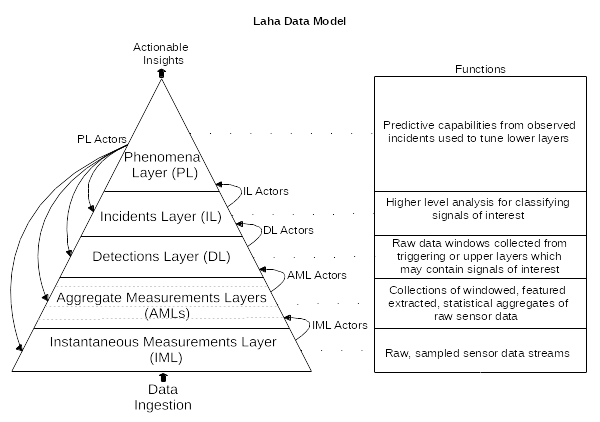
\includegraphics{figures/laha_abstract_overview.png}
	\label{laha-abstract-overview}
\end{figure}

The Laha framework provides two important benefits to DSNs:

\begin{enumerate}
	\item Converts sensor data into actionable data and insights
	\item Provides graceful degradation and metrics on storage requirements for voluminous sensor data
\end{enumerate}

Although not the main focus of this dissertation, Laha provides several tangential benefits with respect to the following DSN problem domains:

\begin{enumerate}
	\item Triggering optimizations
	\item Detection and classification optimizations
	\item Topological optimizations
	\item Sensor energy requirement optimizations
\end{enumerate}

These tangential benefits are provided by Laha Actors that exist within each level of the Laha framework. I do not claim that these techniques are novel, but I do claim that either all or a subset of these techniques are required to enable progress towards the main goals of this framework. To that end, Laha Actors implement several state of the art algorithms present in the literature that address these tertiary problems.

Laha was evaluated by designing and implementing two Laha-compliant reference implementations, OPQ and Lokahi. Open Power Quality (OPQ) is a power quality (PQ) network consisting of custom hardware and distributed software services that detect distributed PQ signals such as voltage sags and swells, frequency sags and swells, transients, THD, and other known PQ issues. OPQ Mauka is a distributed, plugin based middleware component of OPQ that performs higher level analysis, data management, and optimizations of the OPQ services. Lokahi is a distributed infrasound network consisting of mobile iOS and Android devices and multiple cloud based software services whose purpose is to supplement the International Monitoring System (IMS) in detecting large infrasound signals.

The reference implementations were designed and  deployed to test sites at UH Manoa and at the Infrasound Laboratory in Kailua-Kona, Big Island and abroad.

Data collected from the PQ network was validated against calibrated reference sensors that have already been installed at the power mains of a subset of buildings on campus. The Office of Energy Management at UH Manoa has given us full access to live and historic PQ data collected at these reference sensors. OPQ Boxes were co-located and placed in buildings with the reference sensors so that I could validate that the triggering and raw data streams I receive from the OPQ Boxes are in agreement with what the reference sensors are observing.

Data collected from the infrasound network was also validated against industry standard calibrated B\&K infrasound sensors. Further, signals in the infrasound network are known a priori since I am able to control the signals that are generated from our calibrated infrasound source, allowing further validation of received signals.

In order to evaluate the generality of the Laha framework, two separate Laha-compliant DSNs sensing different domains were designed, distributed, and evaluated.

The first Laha-compliant DSN is Open Power Quality (OPQ), a distributed DSN that collects and analyzes power quality (PQ) signals. PQ is a measure of the ``goodness" of the power feeding your electronics. The features that this network collects includes voltage, frequency, and THD. From these features, OPQ can classify the following PQ signals: voltage dips/swells, frequency dips/swells, high levels of THD, and transients. Another goal of this network is to detect distributed PQ signals. That is, the same signal detected on multiple sensors enables one to study how PQ signals move through a power grid. This network provided metrics on the number of Incidents classified as well as numbers of correct predictions from Phenomena. The number of classified Incidents are compared to industry standard PQ monitors co-located with OPQ sensors as a means of evaluating whether Laha is capable of supporting the goals of this network.

The second Laha-compliant DSN is Lokahi, a distributed, mobile infrasound detection network. Infrasound consists of sounds waves that are less than 20 Hz. These signals are generated by large movements of the atmosphere and can be observed from large distances. Examples of infrasound sources include volcano eruptions, meteors, missile launches, and large explosions. In this network, Android and iOS devices were deployed with a special app that is capable of collecting acoustic signals as they travel through the atmosphere. As part of the evaluation, in this network, we collected and discriminated infrasound signals from different types of infrasound sources. Many of these signals are correlated with industry standard infrasound sensors to show that Laha is capable of supporting the infrasound detection goals of this network.

In order to evaluate the multi-level representation of the Laha Framework in the context of providing actionable data, I examined cyclical and predictable signals and tested whether or not Laha is able to utilize predictive analytics to provide actionable insights. To test this, I provided a number of false positive and false negatives for predictive analytic results. I evaluated whether the sensing domain has any effect on how well Laha is able to provide actionable insights. I also claim that each level in the Laha-hierarchy is important in the process of deriving these insights. I provided data that either supports or opposes the usefulness of each level, whether the current number of levels is adequate, and whether the idea of using levels to provide actionable insights is useful at all.

I evaluated my claim that a tiered TTL approach to sensor data management provides the benefits of providing an configurable upper bounds on storage requirements for each Laha level, graceful degradation, and a reduction of sensor noise being stored. To test this, I implemented procedures for calculating storage bounds and determined whether these theoretical bounds are valid in practice. Since it is possible that the TTL approach could throw away important data, I measured the number of false positives using the TTL approach as a means of evaluating its usefulness with a discussion of how detrimental these false positives might actually be to understanding and creating actionable data sets.

Finally, I evaluated multiple state of the art algorithms current in the literature for optimizing triggering, detection, classification, sensor energy usage, and topological modeling and provide metrics to their usefulness for making progress towards the larger goals of providing a generally useful representation for DSNs, converting primitive sensor data into actionable insights, and providing a tiered approach to DSN data management and storage requirements. I provided a discussion on whether these techniques are useful within the two domains that they are implemented, and then, how they contributed to the overall goals of this framework. I also show which combinations of tertiary techniques provide the most traction in solving the overall goals of this framework.

\section{Claims of Laha Abstract Framework}\label{sec:anticipated-contributions-of-laha}

\begin{tcolorbox}
The major claim of this dissertation is that the Laha Framework provides a generally useful representation of an abstract framework for real-time high-volume DSNs. I provide four related claims with design, evaluation, and results for each claim.
\end{tcolorbox}

\subsection{Generality of the Laha Framework}\label{subsec:generality-of-the-laha-framework}
The generality of the framework examines the ability for Laha to be a useful abstract framework in different domains while still meeting the requirements of those domains. This dissertation examines two domains, distributed power quality monitoring through the Open Power Quality network and distributed infrasound monitoring through the Lokahi Network.

To evaluate the generality of the network, I designed, implemented, and deployed two Laha-compliant reference networks in two different domains, power quality and infrasound. The design of these networks is described in Chapter~\ref{ch:system-design}. These reference implementations generate evidence for the ways in which Laha supports the goals of the sensor networks and ways in which it falls short. The evaluation of the generality of Laha is provided in the Evaluation chapter in Section~\ref{sec:use-laha-deployments-to-evaluate-the-main-goals-of-the-framework}. Results showing the generality of Laha are provided in the Results chapter in Section~\ref{sec:results-of-generality-of-this-framework}. The implementations also provide insights into the types of distributed sensor networks for which Laha is well-suited, and the types for which it is not. These insights are discussed in Section~\ref{subsec:discussion-on-types-of-dsns-laha-is-suitable-for}.

\subsection{Ability to Convert Primitive Data into Actionable Insights}\label{subsec:ability-to-convert-primitive-data-into-actional-insights}
Laha uses a tiered hierarchy to convert primitive data into actionable insights. As data passes ``upward" through the levels, context is applied to the data allowing different types of analysis to be performed on the data and more accurate conclusions to be drawn from the data.

The reference implementations enabled me to evaluate the multi-level representation system of tiered levels as described in the Evaluation Section~\ref{subsec:evaluation-of-converting-primitive-data-into-actionable-insights}. I claim that Laha enables a distributed sensor network to derive actionable insights from low level data, and that each of the levels is important to that process. The two reference implementations provide concrete data as to the set of levels that are useful in practice, or whether different levels would be more appropriate, or whether the level strategy itself has problematic features. These results are provided in Sections~\ref{sec:results-of-converting-primitie-data-into-actional-insights} and~\ref{subsec:discussion-of-laha-levels}.

\subsection{Tiered Big Data Management}\label{subsec:tiered-big-data-management}
Laha additionally uses the tiered hierarchy to provide management of ``big data" relating to sensor acquisition and analysis. This is accomplished by providing a Time-to-Live (TTL) value for data that determines when that data should be garbage collected. I show how this approach is able to throw away noisy data while still identifying signals of interest.

I claim that a benefit of Laha's mechanism for managing data is that it enables the calculation of upper bounds on data storage requirements given the state of the network. I developed the analytical procedures required for calculating data storage requirements (as discussed in the Evaluation Section~\ref{subsec:eval-big-data}), and determined whether these procedures are valid in practice as shown in the Results Section~\ref{sec:dsn-system-requirements}. One obvious problem with a TTL approach is the possibility of false negatives: data that is discarded before it has been recognized as important. To quantify my results, I provide a comparison to ground truth sensors as described in the Evaluation Section~\ref{sec:validate-data-collected-by-laha-deployment} and shown in the Results Section~\ref{sec:ground-truth-analysis}.

\subsection{Tertiary Goals and Claims}\label{subsec:tertiary-goals-and-claims}
Finally, I assessed the ability to solve the tertiary problems of optimizing triggering, detection, classification, bandwidth, predictive analytics, and the ability to build a model of the sensing field. I claim that these problems need to be addressed in some form in order to solve the larger problems of turning primitive data into actionable insights and to provide a mechanism for managing large amounts of sensor data. I compare and contrast state of the art algorithms present in the literature to determine if they are effective in practice and useful for addressing the two larger problems. My evaluation in Section~\ref{sec:evaluation-of-tertiary-goals} describe metrics required for demonstrating effectiveness. The results of the tertiary goals are provided in the Results Section~\ref{sec:results-of-tertiary-goals}.

\section{Contributions of Laha}\label{subsec:anticipated-contributions}
I have provided the following four contributions to the areas of DSNs, specifically regarding the problems of optimization and management of DSNs.

First, the Laha design, a novel abstract distributed sensor network that provides two useful properties relating to data management, converting primitive data to actionable data and tiered management of Big Data (Design~\ref{ch:system-design}, Evaluation~\ref{subsec:evaluation-of-converting-primitive-data-into-actionable-insights}, \ref{subsec:eval-big-data}, Results~\ref{sec:results-of-converting-primitie-data-into-actional-insights}, \ref{sec:dsn-system-requirements}).

Second, an evaluation of the Laha abstract framework through the deployment of two Laha-compliant reference implementations, validated data collection, and several experiments that are used to either confirm or deny the benefits claimed by Laha (Evaluation~\ref{sec:validate-data-collected-by-laha-deployment}, Results~\ref{sec:ground-truth-analysis}).

Third, two Laha-compliant reference implementations, OPQ and Lokahi, which can be used to form DSNs for the collection of distributed power quality signals and the distributed collection of infrasound signals. (Design~\ref{ch:system-design}, Evaluation~\ref{sec:deploy-laha-reference-implementations-on-test-sites}, \ref{subsec:evaluation-of-the-generality-of-this-framework}, Results~\ref{sec:results-of-generality-of-this-framework})

Fourth, a set of implications for modern distributed sensor networks as a result of the evaluation of Laha. That is, how does the confirmation or denial of Laha's benefits affect the field of modern DSNs moving forward? Results for these contributions can be found in Sections~\ref{subsec:discussion-on-types-of-dsns-laha-is-suitable-for} and ~\ref{subsec:discussion-of-laha-levels}.

\section{Organization of this Dissertation}\label{subsec:organization-of-this-dissertation}

Chapter~\ref{ch:introduction} introduces the the problem statements (Sections~\ref{sec:converting-sensor-data-into-actionable-insights} and~\ref{sec:big-data-management-in-dsns}), major components of the Laha abstract framework (Section~\ref{sec:laha:-an-abstract-framework-for-adaptively-optimizing-dsns}), traditional approaches to DSN optimization (Section \ref{sec:traditional-approaches-to-dsn-optimization}), contributions to the field of DSNs (Section~\ref{subsec:anticipated-contributions}), and major claims (Section \ref{sec:anticipated-contributions-of-laha}).

Chapter~\ref{ch:related-work} provides a literature review. Section~\ref{sec:big-data-and-distributed-sensor-networks} examines the literature on Big Data and DSNs. Literature on data management related to DSNs is provided in Section~\ref{sec:distributed-sensor-networks-and-big-data-management}. Section~\ref{sec:distributed-sensor-networks-and-predictive-analytics-and-forecasting} discusses literature on predictive analytics and forecasting. Section~\ref{sec:determining-topology-and-localization} examines literature on topology and localization. Section~\ref{sec:optimizations-for-triggering} discusses literature for optimizations for triggering.

Chapter~\ref{ch:system-design} outlines the Laha system design. Section~\ref{sec:big-data-management} provides the design of Big Data management. Section~\ref{sec:phenomena} examines the design of Phenomena. Section~\ref{sec:laha-actors:-acting-on-the-laha-data-model} provides the design of Laha Actors. Section~\ref{sec:opq:-a-laha-compliant-power-quality-dsn} discusses the design of the OPQ network. Finally, Section~\ref{sec:lokahi:-a-laha-compliant-infrasound-dsn} describes the design of the Lokahi network.

Chapter~\ref{ch:evaluation} provides an evaluation of Laha. Section~\ref{sec:deploy-laha-reference-implementations-on-test-sites} examines the deployments for the OPQ and Lokahi networks. Section~\ref{sec:validate-data-collected-by-laha-deployment} discusses evaluation techniques for data validation. Section~\ref{sec:use-laha-deployments-to-evaluate-the-main-goals-of-the-framework} examines strategies for evaluating the main goals of Laha. Section~\ref{sec:evaluation-of-tertiary-goals} provides the evaluation of tertiary goals.

Finally, Chapter~\ref{ch:results} provides results and discussions of results. Section~\ref{sec:ground-truth-analysis} provides results of data validation. Section~\ref{sec:results-of-generality-of-this-framework} discusses results for the generality of the Laha framework. Section~\ref{sec:results-of-converting-primitie-data-into-actional-insights} provides results detailing the conversion of primitive data into actionable insights. Section~\ref{sec:dsn-system-requirements} provides results for tiered management of Big Data. Section~\ref{sec:results-of-tertiary-goals} provides results of Laha's tertiary goals.

Chapter~\ref{ch:conclusion} provides concluding remarks and future directions. Section~\ref{sec:future-directions} outlines future directions. Future directions includes utilizing machine learning to improve triggering, detection, classification, and Phenomena, experimenting with window sizes and thresholds used in detection and classification algorithms, modifications to the Laha level hierarchy, data fusion, more complete simulations, metric collection, and the deployment of larger distributed sensor networks.










\chapter{Related Work}\label{ch:related-work}
This chapter reviews research related defining Big Data in terms of DSNs, Big Data management, self-optimizing DSNs, predictive analytics and forecasting, optimizations to triggering, detection, and classification of signals-of-interest within the context of DSNs.

\section{Big Data and Distributed Sensor Networks}\label{sec:big-data-and-distributed-sensor-networks}
``Big Data" is a term that is used to define either the characteristics of collected data or the processes involved for storing and analyzing collected data. Information that is considered Big Data provides a number of challenges.

One of the best reviews on Big Data literature is provided by the President's Council of Advisors on Science and Technology (PCAST) in their report to the White House~\cite{house2014big}. In this review, Big Data is described using several definitions.

The first definition includes ``high-volume, high velocity, and high-variety information assets that demand cost-effective, innovative forms of information processing for enhanced insight and decision making"~\cite{gartner_it_glossary_2016}. This definition focuses on the characteristics of the data that make it ``Big". In this context high-volume refers to the total amount of data that requires processing, high-velocity refers to the speed at which data arrives, and high-variety refers to the fact that sensor data is often heterogeneous and incomplete. The second part of the definition includes the terms cost-effective, innovative forms of information processing for enhanced insight and decision processing, which implies that we need technology that is able to deal with these types of data characteristics while doing so within the limits of a system with the goal of refining the data to provide insights and decision making that would not have been possible without the information processing.

A second definition~\cite{ward2013undefined} mentioned by the PCAST report rings more true to what Laha attempts to accomplish within the context of DSNs and says that Big Data is ``a term describing the storage and analysis of large and/or complex data sets using a series of techniques including, but not limited to, NoSQL, MapReduce, and machine learning". This second definition defines Big Data in terms of storage and analysis techniques and is a useful definition for describing the processes by which Laha and the Laha reference DSNs deal with distributed sensor data.

Finally, Bhat~\cite{bhat2018data} shows that the production of ``Big Data" is greatly outpacing the available storage for that data. The author shows evidence that even with technological advances is data storage mediums, that the gap still exists. Further, the author shows that there are several shortcomings with current data reduction techniques such as compression and deduplication. Issues with compression include that fact that while lossy compression provides better compression ratios, data quality is reduced and using lossless compression algorithms does not provide the required compression ratios. Compression also provides additional overhead in terms of CPU utilization. Similar to compresses, deduplication shifts the costs from the network to the CPU. As such, other techniques should be considered for data reduction.

\section{Distributed Sensor Networks and Big Data Management}\label{sec:distributed-sensor-networks-and-big-data-management}

Garcia-Gil et al.~\cite{garcia2019enabling} introduce the concept of ``Smart Data" which is value and veracity added to data by means of removing noise from ``Big Data". The authors claim that applying labels to data through classification algorithms are more accurate when noisy data is removed from the initial data set. In order to remove noise, the authors train two different models against noisy and non-noisy data. The authors provided two different approaches to this process both using Apache Spark to distribute the processing load. The first approach the Homogeneous Ensemble for Big Data (HME-BD) which uses a single random forest classifier. The authors also provided a second approach called the Heterogeneous Ensemble for Big Data (HTE-BD) which utilized multiple classifiers for identifying noisy data, namely random forests, logistic regression, and k-nearest neighbors. The authors found the HME-BD approach provided more accurate results and better performance characteristics.  The authors found that by removing noisy data, they were able to increase the accuracy of the classification algorithms.

There are many technologies for movement, transformation, and storage of sensor data. Current state of the art technologies include distributed streaming and computation engines such as Apache Kafka~\cite{kreps2011kafka} or Apache NiFi~\cite{noauthor_apache_nodate}. Although these frameworks provide a lot of flexibility in terms of transformations applied and data management, they do not provide automatic mechanisms for data management. Other, less known technologies are discussed in~\cite{hughes2016survey}, but also suffer from the fact that they are flexible in moving large amount of data, but do nothing to address storage requirements or graceful degradation.

Another approach is to use compression techniques, such as those described by Tang~\cite{tang2004compression}. Tang utilizes spatio-temporal correlation to reduce the amount of data that is transferred from a set of distributed sensors. Tang uses these application specific algorithms to reduce the overall size by a factor of 8 while still maintaining the target signal-to-noise ratio required by the network. However, at scale, even data compression can not keep up with the approach of storing everything all the time.

There are many distributed computation engines and techniques which provide a generic framework for distributing computational tasks across multiple CPUs and multiple machines. The two, which are generally receiving the most academic attention are MapReduce~\cite{dean2008mapreduce} and Apache Spark~\cite{zaharia2016apache}. Although these computation engines are very generic and quite powerful, they can not easily inherit any of the optimizing benefits provided by Phenomena in the Laha framework.

The data grid~\cite{chervenak2000data} is a framework that was designed to provide two basic services the authors believe are fundamental for distributed management and analysis of large scientific datasets, storage systems and metadata management.

Wu~\cite{wu2014data} constructs the HACE framework, which is specifically designed for mining of insightful data from varied Big Data sets. Although this framework is useful for managing multiple streams of data and mining over multiple features, it does not attempt to provide an upper bounds on storage requirements or provide graceful degradation in the face of large scaling networks.

In terms of frameworks using aggregation to facilitate data reduction, Camdoop designed by Costa~\cite{costa2012camdoop} is a framework that aims to push aggregation techniques from the edge of the sensor network all the way to the sink. Camdoop was able to show positive results in data reduction while still maintaining semantic meaning. However, Camdoop was designed to run over simple data streams (such as word count logs) and it is not known how this system would perform with more primitive types of data. Camdoop was designed to run within CamCube simulations and it's not known how this would run in practice with a real DSN.

Rehman et al.~\cite{ur2016big} created a big data reduction framework and argue that reducing data early in the analytics process can lead to efficient value creation. This framework was designed specifically for enterprise customer Big Data analysis, but I believe some of the core tenants could apply to any Big Data problem. They argue that by performing data reduction early in the process its possible to lower service utilization costs, enhance trust between users and developers, and preserve privacy of users among other benefits.

Luan et al.~\cite{luan2015fog} in their paper on Fog Computing, describe data reduction and aggregation techniques by performing some of a subset of computations and data reduction on the edge of the network, such as in mobile devices (cellphones) or in servers that geographically located near the data acquisition sources. Aggregated data is then sent from the edge devices to data sinks for further analysis or action. One of the major difficulties with this approach is handling scale and being able to dynamically deploy resources to the edge as data streams scale.

In a paper by Stateczny et al.~\cite{stateczny2014self}, the authors work to determine whether artificial neural networks can be used to provide Big Data Reduction for hydrographic sonar data. The authors found that they were able to see some reduction, but ran into issues when the data was very dense. The research presented here also appears to be very domain specific.

\section{Distributed Sensor Networks and Predictive Analytics and Forecasting}\label{sec:distributed-sensor-networks-and-predictive-analytics-and-forecasting}

Mohsenian-Rad et al.~\cite{mohsenian2018distribution} designed the $\mu$PMU (phase measurement unit) system which provides distributed power quality measurements over power grid distribution systems. The $\mu$PMUs in conjunction with their backend software provide two types of analytics. Descriptive analytics provide information about the types and classifications of power quality issues that are observed within the power distribution grid. Predictive analytics are used to predict future power quality issues. The authors describe their system as providing the ground for for enabling future prescriptive analytics, which is the idea of self-tuning the DSN to prepare for future power quality problems by using a combination of descriptive and predictive analytics. Prescriptive analytics are a concept that currently exist within the Laha framework.

Anastasi et al.~\cite{anastasi_energy_2009} breaks data predictions algorithms for DSNs into two classes. The first class of algorithms are defined as stochastic approaches and use random probabilities and non-precise statistics to provide predictions. The other class is called time series forecasting and uses historical time series data to provide future predictions. An example of a stochastic model for predicting sensor data is the Ken model~\cite{chu2006approximate} which was developed for energy reduction by minimizing the data sent between sensors and sink nodes. This is accomplished by using a model of sensed data and only sending data when the sensed values at the sensor do not match what was predicted by the model. The model is built during a training phase in which a probabilistic density function (PDF) is generated for the model. Ken is flexible enough to provide models for different types of sensed phenomenon and can work anywhere where there are high correlations in time and space.

Time series forecasting algorithms typically use moving average, auto regressive, or auto regressive moving average models. The authors of the PAQ framework~\cite{tulone2006paq} use auto-regression techniques to build a model of sensor readings that is compared between sensor node and sink nodes while  providing provably correct error bounds. The SAF architecture~\cite{tulone2006energy}, by the same authors, improves on the PAQ framework by refining the AR models and also adds the ability to not only detect outliers, but also detect inconsistent data. These approaches provide predictions for a single feature, however Laha provides the ability for DSNs to be multi-modal. The paper presented by Le et al.~\cite{le2007adaptive} uses time series forecasting, but provides multiple models that are switched out when the data changes. That is, given the current state of the network, a model is selected that is most likely to provide correct predictions. This is useful if a network has multiple features that can be used for forecasting.

Han et al.~\cite{han1999efficient} create an approach for efficient mining of partial periodic patterns in time series databases. Research before this could only match periodic signals if the patterns were completely full, however the authors augment this approach to support the finding of partial periodic signals, which are more common in practice. The authors show that the signals can be recognized after 2 passes of the database. Keogh et al.~\cite{keogh2002finding} take a different approach with their Tarzan algorithm and instead of mining for known periodic signals, they come up with an approach to enumerate all ``surprising" patterns of data in time series databases. They use a statistical approach (a subset of the stochastic approach) that works in linear time to determine if the occurrence of a data point differs from that expected by change. They found that their approach was more sensitive and selective than other approaches described in the paper.

\section{Determining Topology and Localization}\label{sec:determining-topology-and-localization}

Several recent papers have been published for determining the location source of infrasonic signals of interest. These include papers by Pilger et al.~\cite{pilger2019large} for tracking large meteoroids using the International Monitoring System (IMS), Hupe et al.~\cite{hupe2019can} for utilizing IMS to contribute to gravity wave measurements, and Farges et al.~\cite{farges2019infrasound} for localization of lightning strikes using infrasound detections through the IMS. The one commonality between all of these research projects is that they utilize the IMS system for collecting their measurements. The IMS is a large, multi-national effort for creating a high uptime network for detecting nuclear proliferation. This dissertation will show the viability of creating an inexpensive DSN that rivals the IMS using common off the shelf equipment.

Langendoen and Reijers~\cite{langendoen2003distributed} provide comparisons for localization techniques of large DSNs. This approach requires that the DSNs are self organizing and do not depend on global infrastructure (such as GPS), are tolerant to node failures, and are energy efficient. These constraints rule out other localization approaches such as GPS. One thing that differentiates Laha networks to Langendoen's is that Langendoen assumes a random distribution of sensor nodes where sensors in Laha networks are strategically placed. If there are a fraction of nodes that do know their location (anchor nodes), then there are several techniques that meet Langendoen's criteria including Ad hoc Positioning System from Niculescu et al.~\cite{niculescu2003ad}, the N-hop Multilateration Primitive by Savvides et al.~\cite{savvides2002bits}, and Rabaey's work on robust positioning algorithms~\cite{rabaey2002robust}. The three approaches all use three similar phases for localization: distance between anchor nodes and other sensors, position, and refinement. Laha hopes to provide sensor distance between sensors rather than physical distance. The above algorithms use flooding of the network for evaluate distance metrics, which may not be possible in Laha deployed networks.

When timing synchronization between nodes is sufficient, that is, the synchronization between sensors provides a timing accuracy of more than the Nyquist frequency for the signals of interest trying to be captured, it is possible to use arrival time of signals to provide metrics on sensing field topology and localization. This is the premise behind sets of algorithms that look at a single signal and the arrival times of that signal at multiple sensors along with possible direction and then attempt to provide an estimate of source signal localization. This has been performed in infrasound networks using the INFERNO framework as described by Perttu~\cite{perttu2013regional} and in other acoustic DSNs such as those used for efficient shooter localization (finding the source of a gun shot from collected acoustic signatures) in~\cite{gezici2005localization} and~\cite{maroti2004shooter}. Localization of non-acoustic signals has also been shown in the literature. For example, Parsons et al. provide a method for localizing PQ disturbances by analyzing energy flow and peak instantaneous power for both capacitor energizing  and voltage sag disturbances from sampled voltage and current data~\cite{parsons1998direction}.

Although not related to determining the topology of a PQ network, there is research that can also find the optimal placement of PQ sensors given a the topology of the network. Won, et al.~\cite{won2008optimal} provide an automatic method of placing PQ sensors on a known topology to maximize signal collection while minimizing the total number of required sensors.

\section{Optimizations for Triggering}\label{sec:optimizations-for-triggering}
Triggering is the act of observing a feature extracted data stream for interesting features and triggering sensors to provide raw data for a requested time window for higher level analysis. Adaptively optimizing triggering is a way to tune triggering algorithms and parameters with the aim of decreasing false positives and false negatives. In this context, a false positive is triggering on a data stream that does not contain a signal of interest and a false negative is not triggering on a data stream that does contain a signal of interest.

Many of the optimizing triggering algorithms present in the literature exist to minimize sensor energy requirements and bandwidth requirements. This is addressed in great detail in the literature review by Anastasi et al.~\cite{anastasi_energy_2009}. This is accomplished by reducing communications between sensor nodes and the sink. It is argued in~\cite{pottie2000wireless} that the costs of transmitting a single bit of information from a sensor cost approximately the same as running 1000 operations on that sensor. However, there is some contention on this topic as~\cite{alippi_adaptive_2010} argues that in some modern sensors computational requirements can equal or eclipse those of  sensor communication.

One of the main drivers of optimization of triggering is to take advantage of the known sensing field topology of a DSN. This is often referred to in the literature as ``topology control"~\cite{santi2005topology}. When the topology of the sensing field is known and when there is an adequate density of sensors, Vuran et al.~\cite{luan2015fog} show that sampled data display strong spatial and temporal correlations. This fact can be used to reduce the amount of duplicate sensor data that is transmitted, stored, and processed. Topology control is generally split into two categories, ``location  driven" where the location of the sensor is known and ``connectivity driven" which aims to dynamically activate or deactivate sensors to provide complete coverage of a sensing field. Many of the location based approaches in the literature attempt  to maximize the ability for sensors to communicate with each other, however Laha takes the approach that all sensors communicate directly with sink nodes eliminating the need for optimizing intra-sensor communications. One downside to location based approaches is that GPS sensors can be energy hogs and only work with directly line of site to the atmosphere. In these cases, a subset of sensors can be supplied with a GPS and the other sensor use additional techniques such as NTP or statistical analysis to determine location~\cite{langendoen2003distributed}.

More details on topology control can be gathered in the reviews by Karl et al.~\cite{karl2007protocols} and Vuran et al.~\cite{vuran2004spatio}.









\chapter{System Design}\label{ch:system-design}
Laha is an abstract framework for distributed sensor networks that provides a means for turning primitive data into actionable insights, tiered management of voluminous amounts of sensor data. Major goals are in part accomplished by augmenting a DSN with the ability to adaptively optimize its bandwidth, detection, and classification.

The Laha framework is made up of five levels that can be viewed conceptually as a pyramid (see Figure~\ref{laha-abstract-overview}). Primitive data entering the Laha framework is located at the bottom of the pyramid. As data moves upward through the levels, noise is discarded, less interesting events are discarded or aggregated into upper levels, events are given more meaning and context, and associations and predictions are made.

\section{Big Data Management in Laha} \label{sec:big-data-management}
Big Data management was outlined in Section~\ref{sec:big-data-management-in-dsns}. The Laha framework acts as an adaptive sieve for filtering noise and uninteresting data collected from a DSN. In this way, each level only passes what it considers interesting to the level above it. In practice, ``higher" levels determine what is interesting and pull data from ``lower" levels. All data at a particular level is garbage collected at specific intervals relating to its important to the DSN\@.

Each level only keeps data for a specified amount of time before it is garbage collected. As data moves up the pyramid, it is generally considered more useful and therefore has a longer Time to Live (TTL), the amount of the time the data lives before it is garbage collected.  When a higher level detects ``something interesting", the data contained in the time window of ``something interesting" is copied into the levels above it and will persist. If this data is not copied into higher levels, then the data will eventually be garbage collected as determined by its TTL. In this way, Laha preserves data from levels if that data is interesting or is associated with interesting data. This also provides graceful degradation of services. The TTL is managed by the overall memory management of the system. Laha Actors are designed to work within the constraints of the TTL at different levels. If a constraint is broken, the Actor logs this issue. TTL can be optimized by Phenomena at each level to either tune for system performance or tune for decreasing of false positives and false negatives at different levels within the Laha hierarchy.

A summary of data management in Laha is provided in Table~\ref{data-managament-table}. It should be noted that the TTL values are default values specifically for the OPQ and Lokahi networks, but these are configurable and dependent on the domain that Laha is deployed within.

\begin{table}[h]
	\centering
	\begin{tabularx}{\textwidth}{lXl}
		\toprule
		\textbf{Level} & \textbf{Description} & \textbf{Time-to-Live (TTL)} \\
		\midrule
		Phenomena Level (PL) & Contextual \& predictive analytics & 2 years \\
		Incidents Level (IL) & Classified signals & 1 year \\
		Detections Level (DL) & Triggered windowed raw data & 1 month  \\
		Aggregate Measurements Level (AML) & Statistical aggregates of raw data  & 2 weeks  \\
		Instantaneous Measurements Level (IML) & Raw sensor data  & 15 minutes \\
		\bottomrule
	\end{tabularx}
	\caption{Summary of data management and context addition in Laha}
	\label{data-managament-table}
\end{table}

\subsection{Instantaneous Measurements Level}\label{subsec:instantaneous-measurements-level}
The Instantaneous Measurements Level (IML) receives raw, sampled data from the DSN. The amount of data received is determined by the sample rate of each device multiplied by the number of fields per sample. Most of the time, devices in the network are mainly sampling noise. A large percentage of the data in this level is destined for garbage collection and data is assigned a short Time to Live (TTL) of 15 minutes by default. Often times, IML data is bounded by the available onboard memory of the sensor.

\subsection{Aggregate Measurements Level}\label{subsec:aggregate-measurements-level}
The Aggregate Measurements Level (AML) is responsible for rolling up IMs from the IML. In general, this level only works with feature extracted data, rather than working with the raw samples. Each Measurement in the AML provides summary statistics over a configurable time window. For example, these can include min, max, mean, median, mode, and variance statistics.

It is possible to breakup the AML into several sub-levels, each with different window sizes. For example, Laha might roll IMs into one minute AMs, then roll one minute AMs into hour AMs, then days, and so on. Each sub-level within the AML can have its own configurable TTL, ensuring long term summary statistics stick around for as long as needed. This provides us a high level view of the network and can provide insights into long term Trends which would not be visible (or available) in the IM data stream.

Similar to IMs, AMs can be saved and copied to the levels above it when interesting data is observed. This ability allows for AMs during these time periods to be stored and saved from the garbage collection process.

At this point in the hierarchy, we are still not providing any context to the data that we are receiving. Context is provided by levels above the AML\@.

\subsection{Detections Level}\label{subsec:detections-level}
The Detections Level (DL) is the first level that provides some context to the data that the database is receiving. This level is responsible watching the feature extracted data streams, and requesting IMs from the IM level. In general, the detection level is meant to be trigger happy\footnote{Pun intended.} and be overly aggressive when determining whether a feature extracted data stream looks interesting.

When a data stream looks interesting, the DL marks a timestamp $N$ seconds before the interesting features and $M$ seconds after the interesting features, where both $N$ and $M$ are configurable within the framework. The goal is to use a time window that catches signals of interest within it. Since these data ranges will be further processed and refined higher in the hierarchy, there is no issue with collecting large amounts of data in this level.

The actual methods of detection are dependent on the characteristics of every individual sensor network. This framework assumes that the detection algorithms are provided by the implementing frameworks.

Similar to other levels, the DL level will have its IMs and AMs copied into levels above it when upper levels observe something interesting in the DL. The Detections level is set to have a TTL of a one month by default. This dissertation uses the terms ``Events" and ``Detections" interchangeably to describe data produced by the DL.

\subsection{Incidents Level}\label{subsec:incidents-level}
Incidents represent classified signals of interest. Incidents are individual classifications for signals of interest and are created by analyzing data from Events. Data from Events may contain multiple Incidents. Individual signals of interest may be classified as multiple Incidents (for example a transient being classified as both a transient and frequency Incidents).

What separates Incidents from Events are the size of the data windows and the ability to classify signals of interest. Whereas Events contain a window that may or may not contain signals of interest, Incidents always contain classified signals of interest. Further, Incidents are always a subset of Event windows. Event windows are defined by thresholds crossing into non-nominal territory, while Incident windows are defined by classification algorithms for the exact start and end of the Incident within the Event window.

For example, the OPQ network may detect frequency deviations in the triggering data stream. These deviations cause an Event to be generated. The Event is further analyzed by Incident algorithms and it is found that the Event data contains multiple frequency deviation Incidents and an excessive THD Incident. Each Incident is a subset of the original Event. As another example, the Lokahi network detects deviations in the infrasound range. These deviations cause an Event to be generated, which when further analyzed by Incident algorithms, it is found that the Event data window contains two atmospheric explosions that are classified as Incidents.

Incidents are expired after one year of storage by default.

\subsection{Phenomena Level}\label{subsec:phenomena-level}
Phenomena are defined as a grouping of sensors, Events, or Incidents that provide additional context based on annotations, locality, periodicity, predictiveness, or similarity. An example of Phenomena would be determining what caused the classified signals observed in the Incidents Level.

Not only do Phenomena provide interesting insight and analytics into the underlying data, but they also provide a means for adaptively tuning the underlying collection, triggering, detection, and analysis of a distributed sensor network.

Phenomena utilize a TTL of 2 years by default.

Phenomena are summarized in Table~\ref{phenomena-summary-table} and discussed in detail in Section~\ref{sec:phenomena}.

Evaluation of utilizing these levels is provided in the Evaluation in Section~\ref{subsec:eval-big-data}. Results are provided in Section~\ref{sec:dsn-system-requirements}.

\section{Phenomena: Providing Adaptive Optimizations in Laha}\label{sec:phenomena}

Phenomena provide context and actionable insights on top of Incidents generated within a DSN. Where an Incident provides a general classification of a signal of interest, Phenomena go beyond general classifications and provide context such as what caused the signal to appear, or identifying other characteristics of an Incident such as if it is cyclic, similar to other Incidents, or identifying an Incident that never would have been observed due to triggering thresholds.

Not only do Phenomena provide context, Phenomena are also responsible for tuning the underlying DSN\@. Phenomena analyze Incidents and then perform optimizations that increase the signal-to-noise ratio while keeping the DSN bounded in terms of CPU, storage, network, and memory performance. Phenomena also collect and store metrics about the DSN in an attempt to provide context about the performance characteristics of the DSN\@.

The following sections investigate the details of Phenomena and how they are implemented within Laha.

\begin{table}[h]
	\centering
	\begin{tabularx}{\textwidth}{lX}
		\toprule
		\textbf{Phenomena} & \textbf{Description} \\
		\midrule
		Annotations & Provide context about an Incident or set of Incidents \\
		Locality & Provides context on how Incidents are related in time and space \\
		Periodicity & Designation for Incidents that exhibit repetitive or periodic behavior \\
		Similarity & Subset of Incidents found using grouping and community detection algorithms \\
		Future & Incidents predicted to occur in the future\\
		\bottomrule
	\end{tabularx}
	\caption{Summary of Laha Phenomena}
	\label{phenomena-summary-table}
\end{table}

Evaluation of Phenomena is provided in Section~\ref{subsec:evaluation-of-converting-primitive-data-into-actionable-insights}. Results of the evaluation of Phenomena are provided in Section~\ref{subsec:results-of-phenomena}.

\subsection{Annotation Phenomena}\label{subsec:annotations-phenomena}
Annotations provide context about an Incident or a set of Incidents. Annotations are generally user provided or sourced from other data sources to provide supporting context to Incidents. For example, Annotations might include ``Cloud Cover", ``Hurricane Hector", ``Dryer Turns On", etc.

In some sense, annotations allow us to label our data sets beyond a simple classification and start looking at causal classifications. Once enough annotations have been assigned to classified Incidents, Laha can used Annotations to attempt to label unknown Incidents with similar characteristics.

Annotations are useful for creating labeled data sets. Although it is a outside the scope of this dissertation to investigate the use of machine learning for signal classification and prediction, annotations provide a path for Laha-based DSNs to implement machine learning on Incidents and Events and Annotations are a useful tool for providing training data.

Annotations can be created through a user interface (View in OPQ and Lokahi View in Lokahi) or algorithmically. Annotations that are created from a user interface are created by users and consumers of the DSN. This occurs when a user knows the cause of an Incident. The user can access the GUI and add an Annotation to a previously created Incident or Incidents. Users can select multiple Incidents for Annotations.

A second approach to creating annotations is algorithmically. For this, we can make use of Similarity Phenomena. When new Incidents are generated, they are compared against the list of Incidents referenced by Annotation Phenomena for similarity. If the Incidents are statistically similar (with better than 75\% probability), then the newly generated Incidents will be Annotated by the same Annotation. In this case, a new Annotation Phenomena is not created, but rather the new Incidents are referenced in the original Annotation Phenomena.

Annotations can be used to tune a DSN by allowing Laha to filter on Incidents with known Annotations. Users may only care about certain types of Incidents, and would prefer to filter out other types of Incidents. As an example, let us say a user of a distributed power quality network has provided an Annotation for Incidents that are generated by their solar panel installation during times of high solar radiance. This Incident may cause power issues locally and as such they are only interested in similar Incidents. The user can specify that Measurements, Trends, Events, or Incidents from their sensor should only be stored if newly created Incidents have the same Annotations that the user is interested in.

\subsection{Locality Phenomena}\label{subsec:locality-phenomena}
Locality provides context on how Incidents are related to each other in both space and time. Laha is able to determine whether classified Incidents are local to a single sensor, to a group of co-located sensors, or global across an entire network. Sensors can be co-located in both the physical sense and also co-located within a sensing field. For example, sensors in a power quality network may be separated by large distance geographically, but co-located through the electrical grid and the grid's topology.

Over time, Locality Phenomena is used to build a model of sensors in relation to each other and to provide a statistical likelihood that co-located sensors will observe the same signal. Locality Phenomena can be used to drive network triggering, detection, and classification thresholds within a distributed sensor network by using this probabilistic model for determining the likelihood that a sensor or sensors will observe a signal of interest.

The Locality of Incidents can be constantly tested. The main approach for determining locality is combining a breadth first search (BFS) with Similarity Phenomena. When a new Incident is generated, location metadata of the sensors is used to perform a BFS of all other sensors by latitude and longitude. This is done because other sensors may have seen a similar signal of interest, but did not trigger an Event due do the signal not passing any triggering thresholds. When an Incident is triggered by a sensor or multiple sensors, for each sensor that was originally triggered a BFS is used to trigger the nearest neighbor of each of the triggering sensors. The newly triggered data is compared using Similarity Phenomena to determine whether the same signal was observed in the newly triggered sensors. This process takes place recursively until sensors triggered by the BFS no longer contain the signal of interest.

If Incidents are found using this approach, Locality Phenomena is created that references all sensors that observed the same signal. These are classified as either local, semi-local, or global depending on the reach of the signal of interest.

The BFS approach works well assuming the signal topology follows the geographic topology. However, this is not always the case. An an example, a distributed power quality network is constrained to the topology of the power grid which may now exactly match the geographic topology. One of the questions of this dissertation is to determine whether a BFS approach is able to accurately identify the locality of events on networks with constrained topologies.

It is possible to determine the locality of signals on networks with constrained topologies. Similarity Phenomena not only look at the similarity of signals by their features, but can also take into account similarity in time. In this way, Similarity Phenomena can mark Incidents as statistically similar if they not only have similar features, but also occur ``close together" in time. This approach will not find signals that do not pass triggering thresholds, but it can identify the locality of Incidents that happen on a constrained topology that would otherwise go unnoticed using the BFS approach.

By understanding the general locality of Incidents and building a statistical model of sensors that often display co-located Incidents, the Locality Phenomena is able to tune both the sensors themselves and triggering thresholds for the network. As an example, let us say two sensors, A and B, often observe the same signals of interest, but sensor B does not pass any of the triggering thresholds for the DSN. Locality Phenomena can dynamically tune the triggering thresholds for sensor B so that it does trigger on the signals of interest that would normally go unnoticed.

Locality Phenomena can also tune the sampling rate or send rate of features from sensors. Certain signals may only be observed at certain sampling rates due to the Nyquist-Shannon sampling theorem\cite{landau1967sampling} which states that signals with a frequency $F$ can only be observed by sampling at at a rate of $2F$. Knowing that signals attenuate as a function of their distance from the source, the sampling rate of sensors can be modified to ensure that signals of interest are captured at a variety of distances from the signal source.

\subsection{Periodic Phenomena} \label{subsec:periodicity-phenomena}
Periodic Phenomena consist of data that exhibits repetitive behavior, that is, the same types of Measurements, Trends, Events, or Incidents appearing in cycles from single or multiple devices. Periodicity allows for the easy creation of Future Phenomena.

Periodic Phenomena allow us to either tune our network to find periodic data or tune the network to ignore periodic data depending on if the periodic signals are of interest. Periodic Phenomena are especially useful in conjunction with Annotation Phenomena as Laha can assign causality to the periodic signal.

Periodic Phenomena are identified using the following approach. Using a configurable interval, the Periodicity Plugin loads Measurements and Trends for all active sensors over a configurable time window. A time window of 24 hours (the default TTL of Measurements) is used to find periodic signals in Measurements. A time window of two weeks (the default TTL of Trends) is used to find periodic signals in Trends. Larger time windows can be used for Events, Incidents, and Phenomena.

For each feature in the Measurement and Trend data (e.g. frequency, voltage, and THD), the Periodicity plugin first removes the DC offset from the data by subtracting the mean. Next, the plugin filters the signal using a 4th order high-pass filter to filter out noise. The plugin then performs autocorrelation on the signal followed by finding the peaks of the autocorrelation. The mean distance between the peaks of the autocorrelation ($\mu$) provides the period of the signal.

Periodic Phenomena are instrumental in creating Future Phenomena. Periodic Phenomena are used to create Future Phenomena which attempt to predict Incident arrivals at future dates. Periodic Phenomena produce Future Phenomena for all devices that are shown to be periodic. Periodic Phenomena will continue to produce Future Phenomena until consecutive Future Phenomena no longer observe the predicted signals of interest.

\subsection{Similarity Phenomena}\label{subsec:similarity-phenomena}
Similarity Phenomena utilize grouping and community detection algorithms to group Incidents together by their features. Common features used for grouping include time, location, Incident type, Incident duration, or Incident features.

Similarity between signals in a DSN is a difficult problem. Signals attenuate as a function of distance from the source and the topology of the network can also change the shape of the signals. For instance, in a power quality network, signals may change as they pass through the power grid and multiple electronic components. In an infrasound DSN, signals will attenuate based on distance from the source and also change as the signals encounter physical obstacles in the environment (such as hills, man made structures, or even weather patterns).

Because of these difficulties, we can not simply correlate two signals for similarity. Instead, this Phenomena takes multiple approaches to providing statistical similarity between Incidents. The main approach is comparing across high level features. These features include Incident duration and Incident classification. Similarity Phenomena also utilizes Locality, Periodic, and Future Phenomena as weights to determine whether the signals are similar. For example, if signals are periodic, then we can assume that those signals are similar. If signals are local or co-local in reference to Locality Phenomena, then it is more likely that they are similar than comparing two signals that are not generally co-located. If signals are observed from Future Phenomena, then it is more likely that they are similar to previous Incidents that were predicted using the same Phenomena.

To compare the similarity between signals, the above mentioned features are used in combination with community detection algorithms to group similar feature sets. These groupings can be further refined by correlating the signals, but due to the fact that the signal shape may change, these features are weighted less than grouping by high-level features.

K-Means clustering is used on the high-level features to create clusters of related features based on the distance from the mean values of those features. These features include a combination of Incident duration, Incident classification, Incident magnitude, and Sensor location.

\subsection{Future Phenomena}\label{subsec:future-phenomena}
Future Phenomena are a statistical model of the likelihood of seeing an Incident or Incidents at future points in time. Knowing that a signal may occur with some probability allows those affected by those signals time to prepare for the signals.

Future Phenomena are created by a combination of other Phenomena types. The most useful Phenomena for creating Future Phenomena are Periodic Phenomena which forecasts future Incidents based off of periodicity. However, Future Phenomena also take into account other Phenomena. For instance, Future Phenomena uses Locality Phenomena to automatically trigger predicted sensors that often observe the same signals. In this way, Future Phenomena can identify signals of interest that may have not passed various triggering thresholds.

Future Phenomena also make use of Annotation Phenomena to predict signals of interest that have been Annotated. This provides actionable insights into the DSN to predict future causes of signals of interest. As an example, instead of saying that the DSN predicts a voltage sag in a power quality network, the DSN can predict a voltage sag due to a washer machine turning on in the future, providing more context to the DSN\@.

Future Phenomena track three items. The first is a list of sensors that should observe a signal in the future. The second is a list of future times at which a signal of interest should be observed. The final item is a statistical weight that provides the likelihood of observing a future signal of interest. The statistical weight $I$ is given as floating point value between 0 and 1 with 1 being the highest probability and 0 being the lowest probability.

Future Phenomena can also provide dynamic tuning of a DSN in multiple ways. It can either be used to tune the DSN for signals of interest, or it can be used to filter out signals that the user is not interested in. It does this by dynamically modifying the triggering thresholds of sensors that are predicted to observe a signal of interest. In most cases, this means lowering the triggering thresholds of those devices for the predictive time window, making those sensors more sensitive to the expected signal. Future Phenomena can also alter the sample rate and/or receive rate of data from the sensors themselves. The rate can be increased for the predicted time window which does increase the data load, but also decreases the time taken to observe a signal of interest.

Future Phenomena can work the other way as well by increasing triggering thresholds and decreasing sample rates for sensors that are not predicted to observe a signal of interest. In this way, we can reduce the amount of network traffic, CPU utilization, and storage requirements for the network. Of course, by doing this, we increase the odds of missing non-predictive signals of interest. This is a trade-off we are willing to make since predictive signals of interest provide more actionable information than random signals of interest.


\section{Laha Actors: Acting on the Laha Data Model}\label{sec:laha-actors:-acting-on-the-laha-data-model}
Laha Actors act on the Laha hierarchy and provide one of two functions. Actors can move data from one level of the hierarchy upwards through the hierarchy when interesting data is requested by an upper level. Actors can also apply adaptive optimizations downwards through the hierarchy. The Laha framework can support multiple actors at each level. For example, the Incidents Level in our reference power quality network contains actors for each of the following functions: IEEE classified voltage events, frequency variations, power outages, excessive THD, and many others. The Incident Level Actors move data from these Incidents upwards to the Phenomena Level.

Table~\ref{laha-actors-tables} summarizes the actors that exist within the Laha framework and their purposes.

\begin{table}[h]
	\centering
	\caption{Summary of Laha Actors}
	\begin{tabularx}{\textwidth}{lX}
		\toprule
		\textbf{Actor} & \textbf{Purpose} \\
		\midrule
		IML Actors & Perform feature extraction and move aggregate data to AML \\
		AML Actors & Perform triggering on data from IML, copy data to DL if interesting \\
		DL Actors & Perform high fidelity feature extraction on possible detections \\
		IL Actors & Perform classification and contextualization on possible detections \\
		PL Actors & Generate predictive analytics and optimize the lower levels of the hierarchy \\
		\bottomrule
	\end{tabularx}
	\label{laha-actors-tables}
\end{table}

\subsection{Actor Constraints}\label{subsec:actor-constraints}
Actors at each level in the hierarchy are governed by a set of constraints. These constraints include the set of possible inputs, $A_i$, the set of possible outputs, $A_o$, the set of Actors it can receive data from, $A_{ai}$, the set of Actors it can transmit data to, $A_{ao}$, and a set of performance metrics that each actor must maintain, $A_p$. The constraints assigned to each Actor are determined by the hierarchy level in which the Actor resides.

Actors are responsible for reporting constraint violations and in this way, Actors are the primary provider of health, performance, and status metrics about the Laha framework.

The constraints for each level of Laha hierarchy is summarized in Table~\ref{actor-constraint-table}.

\begin{table}[h]
	\centering
	\caption{Summary of Laha Actor Constraints at Each Level}
	\begin{tabularx}{\textwidth}{lXXllX}
		\toprule
		\textbf{Level} & \boldmath{$A_i$} & \boldmath{$Ao$} & \boldmath{$A_{ai}$} & \boldmath{$A_{ao}$} & \boldmath{$A_p$} \\
		\midrule
		IML & Raw samples & Aggregate Trends & n/a & AML & Data ranges available \\
		AML & Aggregate Trends & Detections & IML & DL & Data ranges available \\
		DL & Windowed waveforms & Hi-fi extracted features & AML & IL & Data \& features available \\
		IL & Hi-fi extracted features & Contextualized Incidents & DL & PL & Incident types available \\
		PL & Contextualized Incidents & Optimizations & IL & All levels & Optimizations available \\
		\bottomrule
	\end{tabularx}
	\label{actor-constraint-table}
\end{table}

\section{OPQ: A Laha-compliant Power Quality DSN}\label{sec:opq:-a-laha-compliant-power-quality-dsn}
OPQ Mauka is a middleware component of the Open Power Quality (OPQ) framework. The OPQ project provides a hardware and software solution for monitoring distributed power quality (PQ). The OPQ project was founded with the goal of studying how intermittent distributed renewable energy sources affect PQ not just at a user's home, but also within a user's neighborhood, between neighborhoods, and globally across the grid.

The OPQ ecosystem is made up of networked hardware sensors (OPQ Boxes) and various software services (OPQ Makai, OPQ Mauka OPQ Health, OPQ View). Each of these software components are made up of individual services and plugins. The entire software system is deployed as Docker~\cite{docker:2019} containers.

The OPQ system design is laid out in Figure~\ref{fig:opq-system}.

\begin{figure}
	\centering
	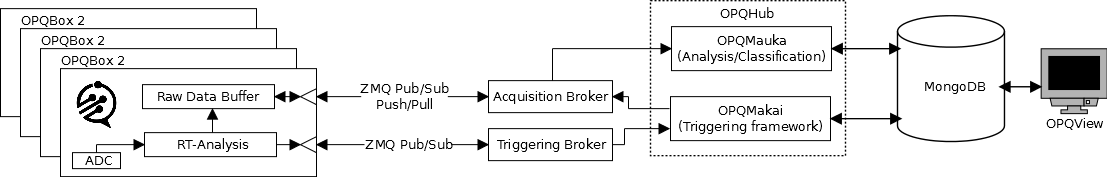
\includegraphics[width=\linewidth]{figures/system-diagram.png}
	\caption{OPQ System Diagram}\label{fig:opq-system}
\end{figure}

\subsection{OPQ: Boxes}\label{subsec:opq:-boxes}
An OPQ Box is a custom designed PQ sensor. OPQ Boxes can be plugged into a wall outlet and communicate with OPQ servers using the user's WiFi connection. OPQ Boxes consist of a Raspberry PI single board computer (SBC), a custom board for PQ measurements, custom firmware, and a custom enclosure. The custom board contains an ADC that samples an alternating current (AC) power signal at 12 thousand samples per second. This data is transferred to the Raspberry Pi where feature extraction and data transfer takes place. The hardware design is presented in Figure~\ref{fig:opq-box-design} and the software design is provided in Figure~\ref{fig:opq-box-software}.

\begin{figure}
	\centering
	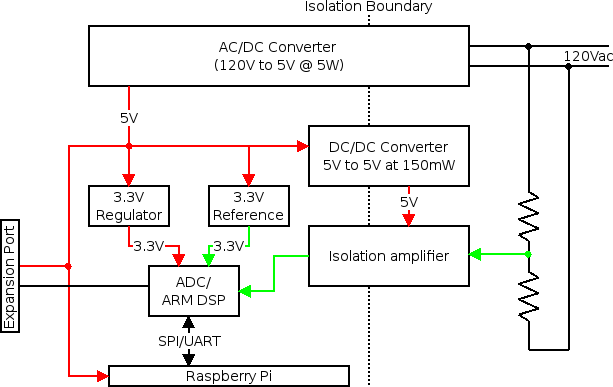
\includegraphics[width=.75\linewidth]{figures/opqbox_diagram.png}
	\caption{OPQ Box Design}\label{fig:opq-box-design}
\end{figure}

\begin{figure}
	\centering
	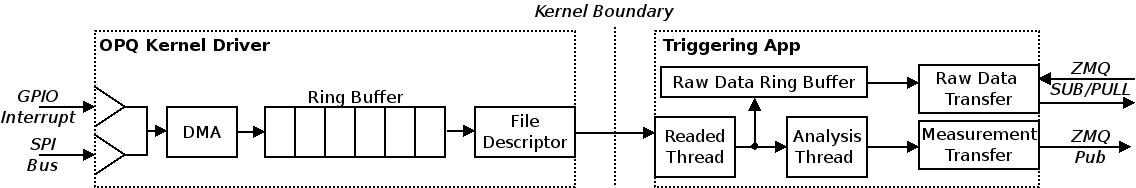
\includegraphics[width=.75\linewidth]{figures/opqbox_software.png}
	\caption{OPQ Box Software}\label{fig:opq-box-software}
\end{figure}

The feature extraction algorithms extract from the sampled waveform the following features: windowed $V_{RMS}$, frequency, and total harmonic distortion (THD) features. The feature extracted data is then sent to a central sink where further analysis is used to determine whether the sensor or a subset of sensors should be triggered for raw data.

The OPQ network is a hybrid network that uses edge computing for calculating features at the edge of the network. This is opposed to networks that utilize a ``send everything" approach. In this way, Laha is able to minimize bandwidth.

OPQ Boxes are synchronized to each other and the OPQ back end using the network time protocol (NTP). This provides synchronization to the millisecond level, which although is great for longer Incidents, does not provide accurate timing for transients that may be shorter than tens of milliseconds.

\subsection{OPQ: Makai}\label{subsec:opq:-makai}
OPQ Makai is the central sink and triggering daemon for the OPQ framework. It is made up of several services which are responsible for aggregating and processing the Measurements generated by OPQ Boxes. Low fidelity feature extracted data consisting of $V_{RMS}$, frequency, and THD are streamed from OPQ Boxes at a configurable message rate. These data streams are observed by OPQ Makai and the daemon uses statistical methods and configurable thresholds to determine whether the sensor or a subset of sensors should be triggered for a window of raw sampled waveforms.

\subsubsection{Dynamic Triggering}\label{subsubsec:dynamic-triggering}

While Makai is mostly implemented by my colleague Sergey Negrashov, I implemented my own triggering logic into Makai to trigger PQ Events. This threshold based triggering is written as a Rust~\cite{rust:2019} plugin for Makai's TriggeringService. The plugin receives a stream of Measurements of OPQ Boxes. Each Measurement contains min, max, and average values for frequency, voltage, and THD over the Measurement's time window.

This plugin checks if a Measurement stream from a Box passes minimum or maximum thresholds for the Measurement's features. Thresholds are provided in the Mongo database in the collection ``makai\_config". The thresholds are provided as minimum and maximum percentages from nominal. For example, the database provides values for nominal voltage and frequency (120$V$ and 60$Hz$ respectively) and thresholds for minimum and maximum percentage from nominal for voltage and frequency. It also checks the maximum percent of THD from 0.

Not only does the database provide default dynamic thresholds for all devices, but it also includes threshold overrides for individual devices. Override thresholds contain the same information as default thresholds, but also include a box\_id. When loading thresholds for a device, if an override does not exist, then default thresholds are used. If an override does exist, then the thresholds from the override are used.

All thresholds are cached for performance reasons. Values from Measurements are compared to these cached thresholds. This is needed so that this plugin does not have to request the thresholds from the database on every Measurement from every Box. Instead, cached values are used. The cache is updated at a configurable interval but defaults to once a minute.

Thresholds are dynamic and can be modified by the ``ThresholdOptimizationPlugin" (described in Section~\ref{subsubsec:threshold-optimization-pugin}) in Mauka.

This plugin utilizes a finite state machine (FSM) which maintains the triggering state for each feature for each Box. There are only three states, ``Check Metrics", ``Metrics Non-Nominal" and ``Trigger Sensor". If a feature for a Box passes a minimum or maximum threshold for a Box feature, then the state for that feature moves from the ``Check Metrics" state into the ``Metrics Non-Nominal" state. The ``Metrics Non-Nominal" state remains in effect until the data is no longer passing the threshold, at which time, a trigger is sent to the sensors requesting data for the time window of the entire ``Non-Nominal" state. Once the trigger has been made, the state transitions back into the ``Check Metrics" state.

From here, Makai handles Event storage and notification of the triggered Boxes.

Figure~\ref{fig:threshold_triggering} provides an overview of the states that are managed by the FSM\@.

\begin{figure}
	\centering
	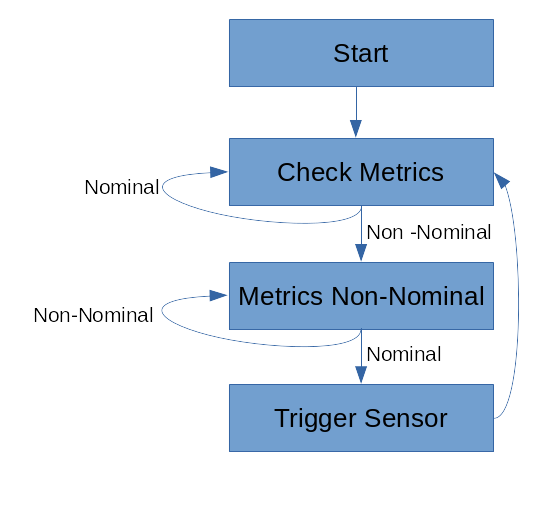
\includegraphics[width=.40\linewidth]{figures/trigger_fsn.png}
	\caption{Threshold Triggering FSM States}
	\label{fig:threshold_triggering}
\end{figure}

\subsubsection{TTL Provider Service}
Time-to-Live (or TTL) is a metric for defining when documents in the Mongo database should be garbage collected. The TTL metric is stored dynamically in the MongoDB collection ``laha\_config". A TTL metric is provided for each collection and the value represents the number of seconds after document creation that that document should be garbage collected. TTLs are dynamically managed by Mauka's ``TtlOptimizationPlugin" (described in Section~\ref{subsubsec:ttl-optimization-pugin}). The actual garbage collection itself is provided by Mauka's ``LahaGcPlugin" (Section~\ref{sec:gc_plugin}).

TTLs are assigned in Makai to Measurements, Trends, and Events since Makai handles storage for these collections. Because TTLs are dynamic and can be updated by Mauka at any time, a cached TTL provider service was created to provide performant access to TTLs in the database. This service loads the TTLs from the database and caches those values for a configurable amount of time (which defaults to one minute). The cache enables Makai to assign TTLs without hitting the database for every Measurement, Trend, and Event that it creates. If a TTL is updated by Mauka, then the cached value will expire after a configurable amount of time and the new TTL will be cached and used until the next cache invalidation.

This service lives within Makai and was written in Rust.

\subsubsection{Event Id Service}
Event Ids are used to uniquely identify Events produced by either Makai or Mauka. We need to ensure that Event Ids are unique between services and monotonically increasing. This constraint requires that a single source of truth provide the Event Ids to avoid race conditions between Makai and Mauka. The EventId Service is a service written in Rust that resides in Makai's Event Broker.

The service wraps an atomic integer and provides thread-safe access to this integer. The service allows any other service within Laha to peak at the current highest Event Id and to also increment and get the next highest available Event Id. When this service is initialized, it queries the MongoDB for the highest Event Id in the database. All other requests to this service will increment the atomic integer and use that value for the next Event Id. In this way, the database only needs to be queried once on initialization and all other operations are on the atomic integer.


This service can be passed directly into Makai's Event Broker using automatic reference counting (ARC). To enable Mauka to access this service, the same service is passed into a ZMQ thread using ARC. The ZMQ thread provides a ZMQ REP endpoint for requesting atomic Event Ids from this service. An example of Mauka requesting the Event Id from Makai is described in Section~\ref{sec:trigger_plugin}.

A high level overview of the Event Id Service is provided in Figure~\ref{fig:eid_service}.

\begin{figure}
	\centering
	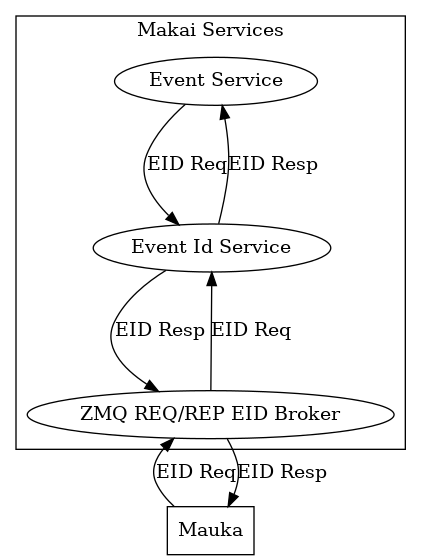
\includegraphics[width=0.4\linewidth]{figures/event_id_service.png}
	\caption{Event Id Service}
	\label{fig:eid_service}
\end{figure}

\subsection{OPQ: Mauka}\label{subsec:opq:-mauka}
OPQ Mauka (or just Mauka) is a middleware component of the OPQ system that provides higher level analytics on PQ data as well as a platform for managing data volume, providing actionable insights into the network, optimizing the network, and providing PQ based Phenomena. Most importantly, Mauka provides most of the functionality that makes OPQ a Laha-compliant DSN\@.

Mauka sits between Makai and OPQ's database. It receives messages from Makai when Makai has triggered OPQ Boxes due to something interesting in the low-fidelity data stream. Mauka then retrieves the raw waveforms stored in the database by Makai, performs feature extraction, and then forwards the features and/or raw waveform to various plugins to perform classification and other high level analytics. These results are then stored in our database and presented to users in OPQ View.

Mauka was written entirely in Python 3.7\cite{python:2019} and relies on various scientific libraries for analytics. These include SciPy\cite{scipy:2019}, numpy\cite{numpy}, matplotlib\cite{matplotlib}, and scikit-learn\cite{scikitlearn}. Communication between processes are accomplished with the ZeroMQ\cite{zmq} library. Messages are serialized using Protocol Buffers\cite{protobuf}. The Mauka code base consists of over 9,594 lines of Python code split over 45 Python modules. The code base is licensed under the GNU General Public License (GPL) version 3\cite{gplv3}. Mauka is hosted and publicly accessible at OPQ's github repository\cite{opqgithub}.

Mauka was designed as a distributed set of processes that communicate via type-safe message passing. Most functionality in Mauka is implemented as plugins where each plugin runs in its own process, providing horizontal scalability. The direction of communication between plugins can be modeled by a directed acyclic graph (DAG). The DAG property of Mauka plugins ensures easy horizontal scalability by making it possible to trivially create many distributed instances of plugins to meet the computational load.

The following sections will detail all components and functionality provided by Mauka.

\subsubsection{Mauka Communication}
ZeroMQ is used to facilitate communication between Mauka and Makai and also between plugins within Mauka. ZeroMQ is a light-weight message queue that provides libraries for many programming languages. ZeroMQ makes it easy to create many different types of communication topologies. However, Mauka mainly makes use of publish/subscribe and push/pull topologies. ZeroMQ is provided to Python using the pyzmq library.

In publish/subscribe, any producer can produce messages where each message contains a topic and a payload. Subscribers are then able to subscribe (or listen to) topics of interest and only ingest messages for topics that they are subscribed to.

The push/pull model on the other hand provides unidirectional message flow from a single pushed to a single puller. Using these two types of communications models in conjunction provides the entire communications backbone for Mauka.

To facilitate communication between Mauka and Makai and between Mauka plugins, two communications brokers are provided. Brokers are separate processes whose only jobs are to manage moving typed messages from a source destination to multiple target destinations.

The first broker, the Makai Event Bridge broker, is responsible for subscribing to a ZeroMQ endpoint provided by Makai. This bridge is used to pass Event Ids created by Makai into Mauka, alerting Mauka to the presence of new data in the database to analyze. When the message is received by the broker, it is transformed into a Mauka Message and published to the second broker, the Mauka Pub Sub Broker, and then broadcast to any subscribing plugins. Mauka plugins that subscribe to Event Ids then use the Event Id to look up the associated raw waveforms in the database to perform analysis.

The second broker, the Mauka Pub Sub broker facilitates message passing between all other parts of the Mauka ecosystem. All messages in this system are published to this broker, and all plugins subscribe to topics provided by this broker. In essence, this broker is used to route type safe messages between distributed components of this system. By using pub/sub and a broker, the plugins only need to worry about one communication endpoint instead of knowing exactly where each plugin lives in the network and how to address it individually.

Figure~\ref{fig:mauka_brokers} provides a high level view of how the brokers facilitate communication between Makai and Mauka as well as between Mauka plugins.

\begin{figure}
	\centering
	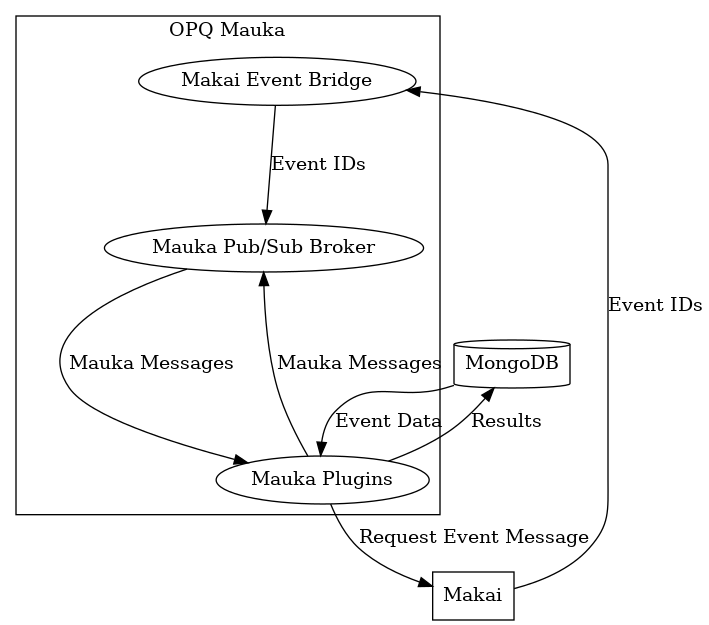
\includegraphics[width=.4\linewidth]{figures/mauka_brokers_communication.png}
	\caption{OPQ Mauka Brokers Communication Diagram}
	\label{fig:mauka_brokers}
\end{figure}

One down side to this approach is that the brokers become single points of failure. I believe that this issue is minimized by using the production proven ZMQ backend for communications. I have also never experienced failures in the broker during data collection or normal system usage.

\subsubsection{Mauka Communication Protocol}
The messages that are passed using ZeroMQ are serialized using the type safe protocol buffers (v3) format. Protocol buffers provide efficient binary serialization/deserialization routines for structured data and can be used from a multitude of programming languages.

Mauka provides a single message type, ``MaukaMessage", that includes many subtypes. All messages passed within Mauka are of the instance MaukaMessage and may include different subtypes. The MaukaMessage protocol is described in detail in the following tables.

The ``MaukaMessage" (Table~\ref{table:MaukaMessage}) type contains a timestamp, source, and a union type which can contain multiple types of type safe messages. Every plugin within Mauka sends and receives MaukaMessages and the plugin is responsible for checking the type of the ``message" field and acting on it.

\begin{table}[H]
	\centering
	\caption{MaukaMessage}
	\begin{tabularx}{\textwidth}{lXX}
		\toprule
		\textbf{Field} & \textbf{Type} & \textbf{Description} \\
		\midrule
		timestamp\_ms & uint64 & Timestamp of message creation.  \\
		source & string & Name of plugin that produced this message. \\
		message & oneof (Payload, Heartbeat, MakaiEvent, Measurement, MakaiTrigger, Laha, TriggerRequest, ThresholdOptimizationRequest, RateOptimizationRequest, TtlOptimizationRequest, Request) & A union of subtypes. \\
		\bottomrule
	\end{tabularx}
	\label{table:MaukaMessage}
\end{table}

The ``Payload" (Table~\ref{table:Payload}) variant of message contains data payloads cast to 64-bit precision floating point numbers. This allows us to work with data of multiple type by assuming all data payloads can be cast to 64-bit floats. This message also contains metadata relating to where the data came from, timing information, and a type safe enumeration describing the type of data stored in the payload.

\begin{table}[H]
	\centering
	\caption{Payload}
	\begin{tabularx}{\textwidth}{llX}
		\toprule
		\textbf{Field} & \textbf{Type} & \textbf{Description} \\
		\midrule
		event\_id & uint32 & Event that this payload originated from.  \\
		box\_id & string & Box that this payload originated from. \\
		data & [f64] & An array of data cast to double precision floats. \\
		payload\_type & PayloadType & Enumeration providing payload type information. \\
		start\_timestamp\_ms & uint64 & Start timestamp of first payload element \\
		end\_timestamp\_ms & uint64 & End timestamp of last payload element\\
		\bottomrule
	\end{tabularx}
	\label{table:Payload}
\end{table}

The ``PayloadType" (Table~\ref{table:PayloadType}) variant is an enumeration that describes the type of data stored in any provided payload.

\begin{table}[H]
	\centering
	\caption{PayloadType}
	\begin{tabularx}{\textwidth}{XlX}
		\toprule
		\textbf{Field} & \textbf{Value} & \textbf{Description} \\
		\midrule
		ADC\_SAMPLES & 0 & ADC waveform samples from the Box.  \\
		VOLTAGE\_RAW & 1 & Raw waveform voltage obtained by dividing ADC values by a calibration constant. \\
		VOLTAGE\_RMS & 2 & RMS waveform obtained by dividing raw voltage by sqrt(2). \\
		VOLTAGE\_RMS\_WINDOWED & 3 & RMS extracted feature array. \\
		FREQUENCY\_WINDOWED & 4 & Frequency extracted feature array. \\
		\bottomrule
	\end{tabularx}
	\label{table:PayloadType}
\end{table}

The ``Heartbeat" (Table~\ref{table:Heartbeat}) variant is a message that is periodically sent from each plugin providing statistics about plugin health.

\begin{table}[H]
	\centering
	\caption{Heartbeat}
	\begin{tabularx}{\textwidth}{llX}
		\toprule
		\textbf{Field} & \textbf{Type} & \textbf{Description} \\
		\midrule
		last\_received\_timestamp\_ms & uint64 & Last time a plugin on\_message was fired.  \\
		on\_message\_count & uint32 & The amount of times on\_message has been fired. \\
		status & string & Custom status message that plugin can override. \\
		\bottomrule
	\end{tabularx}
	\label{table:Heartbeat}
\end{table}

The ``MakaiEvent" (Table~\ref{table:MakaiEvent}) variant is a message which includes the ``event\_id" of a newly created Event from Makai. This message is received by the ``MakaiEventPlugin" and is used to begin processing new Events within Mauka generated by Makai.

\begin{table}[H]
	\centering
	\caption{MakaiEvent}
	\begin{tabularx}{\textwidth}{llX}
		\toprule
		\textbf{Field} & \textbf{Type} & \textbf{Description} \\
		\midrule
		event\_id & uint32 & The Event number that Makai has recorded.  \\
		\bottomrule
	\end{tabularx}
	\label{table:MakaiEvent}
\end{table}

The ``Measurement" (Table~\ref{table:Measurement}) variant is a message that contains an Instantaneous Measurement which includes a timestamp, voltage, frequency, and THD metrics.

\begin{table}[H]
	\centering
	\caption{Measurement}
	\begin{tabularx}{\textwidth}{llX}
		\toprule
		\textbf{Field} & \textbf{Type} & \textbf{Description} \\
		\midrule
		box\_id & string  & Box that this Measurement came from. \\
		timestamp\_ms & uint64 & Timestamp that this Measurement was recorded. \\
		frequency & double & The instantaneous frequency of this Measurement. \\
		voltage\_rms & double & The instantaneous RMS voltage of this Measurement. \\
		thd & double & The instantaneous THD of this Measurement. \\
		\bottomrule
	\end{tabularx}
	\label{table:Measurement}
\end{table}

The ``MakaiTrigger" (Table~\ref{table:MakaiTrigger}) variant is a message type that is used to send to Makai in order for Mauka to trigger Boxes for raw data. This is used when Mauka sees something interesting and wishes to request more data than what was originally provided by Makai.

\begin{table}[H]
	\centering
	\caption{MakaiTrigger}
	\begin{tabularx}{\textwidth}{llX}
		\toprule
		\textbf{Field} & \textbf{Type} & \textbf{Description} \\
		\midrule
		event\_start\_timestamp\_ms & uint64  & The start timestamp of the trigger. \\
		event\_end\_timestamp\_ms & uint64 & The end timestamp of the trigger. \\
		event\_type & String & A string description of the Event (or reason) we are triggering Boxes. \\
		max\_value & double & The maximum value of ``event\_type" observed in the triggering stream. \\
		box\_id & String & The OPQ Box Id. \\
		\bottomrule
	\end{tabularx}
	\label{table:MakaiTrigger}
\end{table}

The ``Laha" (Table~\ref{table:Laha}) message variant contains multiple types of messages all relating to Laha. These include messages for managing TTL, garbage collection, and Laha based statistics.

\begin{table}[H]
	\centering
	\caption{Laha}
	\begin{tabularx}{\textwidth}{lXX}
		\toprule
		\textbf{Field} & \textbf{Type} & \textbf{Description} \\
		\midrule
		laha\_type & Oneof (Ttl, GcTrigger, GcUpdate, GcStat) & Sum type that contains multiple subtypes. \\
		\bottomrule
	\end{tabularx}
	\label{table:Laha}
\end{table}

The ``Ttl" (Table~\ref{table:Ttl}) Laha message variant is used to dynamically specify TTLs for the provided collection.

\begin{table}[H]
	\centering
	\caption{Ttl}
	\begin{tabularx}{\textwidth}{llX}
		\toprule
		\textbf{Field} & \textbf{Type} & \textbf{Description} \\
		\midrule
		collection & String & The data collection type that should have its TTL updated.  \\
		ttl\_s & uint32 & The number of seconds that a collection should have its TTL set to. \\
		\bottomrule
	\end{tabularx}
	\label{table:Ttl}
\end{table}

The ``GcTrigger" (Table~\ref{table:GcTrigger}) variant is a message that is sent to the GC plugin to notify it that GC should be performed on the domains specified in the message.

\begin{table}[H]
	\centering
	\caption{GcTrigger}
	\begin{tabularx}{\textwidth}{llX}
		\toprule
		\textbf{Field} & \textbf{Type} & \textbf{Description} \\
		\midrule
		gc\_domains & [GcDomain] & The data collection type that should have its TTL updated.  \\
		\bottomrule
	\end{tabularx}
	\label{table:GcTrigger}
\end{table}

The ``GcDomain" (Table~\ref{table:GcDomain}) enum is used to specify a garbage collection domain within Laha.

\begin{table}[H]
	\centering
	\caption{GcDomain}
	\begin{tabularx}{\textwidth}{lll}
		\toprule
		\textbf{Field} & \textbf{Value} & \textbf{Description} \\
		\midrule
		MEASUREMENTS & 0 & Laha Measurements.  \\
		TRENDS & 1 & Laha Trends. \\
		EVENTS & 2 & Laha Events. \\
		INCIDENTS & 3 & Laha Incidents. \\
		PHENOMENA & 4 & Laha Phenomena. \\
		SAMPLES & 5 & Laha samples. \\
		\bottomrule
	\end{tabularx}
	\label{table:GcDomain}
\end{table}

A ``GcUpdate" (Table~\ref{table:GcUpdate}) variant is a message that informs the GC plugin to update the TTL for a particular document and all documents living under it.

\begin{table}[H]
	\centering
	\caption{GcUpdate}
	\begin{tabularx}{\textwidth}{llX}
		\toprule
		\textbf{Field} & \textbf{Type} & \textbf{Description} \\
		\midrule
		from\_domain & GcDomain & The GcDomain from which this update originated. All collections under this domain are also updated.  \\
		Id & uint32 & The Id of the document that should have its TTL updated. \\
		\bottomrule
	\end{tabularx}
	\label{table:GcUpdate}
\end{table}

A ``GcStat" (Table~\ref{table:GcStat}) variant message is a message that contains statistics on the number of items garbage collected from a particular GcDomain.

\begin{table}[H]
	\centering
	\caption{GcStat}
	\begin{tabularx}{\textwidth}{llX}
		\toprule
		\textbf{Field} & \textbf{Type} & \textbf{Description} \\
		\midrule
		gc\_domain & GcDomain & The GcDomain from which this statistic originated. \\
		gc\_cnt & uint64 & The count of items garbage collected on the last GcTrigger message.  \\
		\bottomrule
	\end{tabularx}
	\label{table:GcStat}
\end{table}

A ``TriggerRequest" (Table~\ref{table:TriggerRequest}) variant message is a message that is instantiated by Phenomena and sent to the ``TriggerPlugin" enabling Mauka to directly trigger OPQ Boxes for raw data.

\begin{table}[H]
	\centering
	\caption{TriggerRequest}
	\begin{tabularx}{\textwidth}{llX}
		\toprule
		\textbf{Field} & \textbf{Type} & \textbf{Description} \\
		\midrule
		start\_timestamp\_ms & uint64 & Start time of data request. \\
		end\_timestamp\_ms & uint64 & End time of data request. \\
		box\_ids & [string] & An array of Boxes to request data from. \\
		incident\_id & uint64 & The original Incident leading to this trigger request. \\
		\bottomrule
	\end{tabularx}
	\label{table:TriggerRequest}
\end{table}

A ``ThresholdOptimizationRequest" (Table~\ref{table:ThresholdOptimziationRequest}) variant message is a message that is created by Phenomena and sent to the ``ThresholdOptimizationPlugin" to dynamically modify default or override thresholds values for Makai's threshold triggering plugin.

\begin{table}[H]
	\centering
	\caption{ThresholdOptimizationRequest}
	\begin{tabularx}{\textwidth}{XlX}
		\toprule
		\textbf{Field} & \textbf{Type} & \textbf{Description} \\
		\midrule
		default\_ref\_f & f64 & Default reference frequency \\
		default\_ref\_v & f64 & Default reference voltage \\
		default\_threshold\_percent\_f\_low & f64 & Default frequency percent low threshold \\
		default\_threshold\_percent\_f\_high & f64 & Default frequency percent high threshold \\
		default\_threshold\_percent\_v\_low & f64 & Default voltage percent low threshold \\
		default\_threshold\_percent\_v\_high & f64 & Default voltage percent high threshold \\
		default\_threshold\_percent\_thd\_high & f64 & Default THD percent high threshold \\
		box\_id & str & Override Box Id \\
		ref\_f & f64 & Override reference frequency \\
		ref\_v & f64 & Override reference voltage \\
		threshold\_percent\_f\_low & f64 & Override frequency percent low threshold \\
		threshold\_percent\_f\_high & f64 & Override frequency percent high threshold \\
		threshold\_percent\_v\_low & f64 & Override voltage percent low threshold \\
		threshold\_percent\_v\_high & f64 & Override voltage percent high threshold \\
		threshold\_percent\_thd\_high & f64 & Override THD percent high threshold \\
		\bottomrule
	\end{tabularx}
	\label{table:ThresholdOptimziationRequest}
\end{table}

A ``RateOptimizationRequest" (Table~\ref{table:RateOptimizationRequest}) variant message is a message that is instantiated by Phenomena and sent to the ``RateOptimizationPlugin" enabling Mauka to dynamically modify the receive rate of Measurements and Trends for specified Boxes.

\begin{table}[H]
	\centering
	\caption{RateOptimizationRequest}
	\begin{tabularx}{\textwidth}{llX}
		\toprule
		\textbf{Field} & \textbf{Type} & \textbf{Description} \\
		\midrule
		box\_id & str & The Id of the Box to change the receive rate for \\
		measurements\_hz & f32 & Measurements per second \\
		\bottomrule
	\end{tabularx}
	\label{table:RateOptimizationRequest}
\end{table}

A ``TtlOptimizationRequest" (Table~\ref{table:TtlOptimizationRequest}) variant message is a message that is instantiated by Phenomena and sent to the ``TtlOptimizationPlugin" enabling Mauka to dynamically modify the TTL of collections stored in the ``laha\_config" collection.

\begin{table}[H]
	\centering
	\caption{TtlOptimizationRequest}
	\begin{tabularx}{\textwidth}{llX}
		\toprule
		\textbf{Field} & \textbf{Type} & \textbf{Description} \\
		\midrule
		collection\_name & str & Collection to modify the TTL for \\
		ttl & int32 & New TTL for the defined collection in seconds \\
		\bottomrule
	\end{tabularx}
	\label{table:TtlOptimizationRequest}
\end{table}

Figure~\ref{fig:mauka_messages} displays all types used and their variants for the Mauka communications protocol.

\begin{figure}
	\centering
	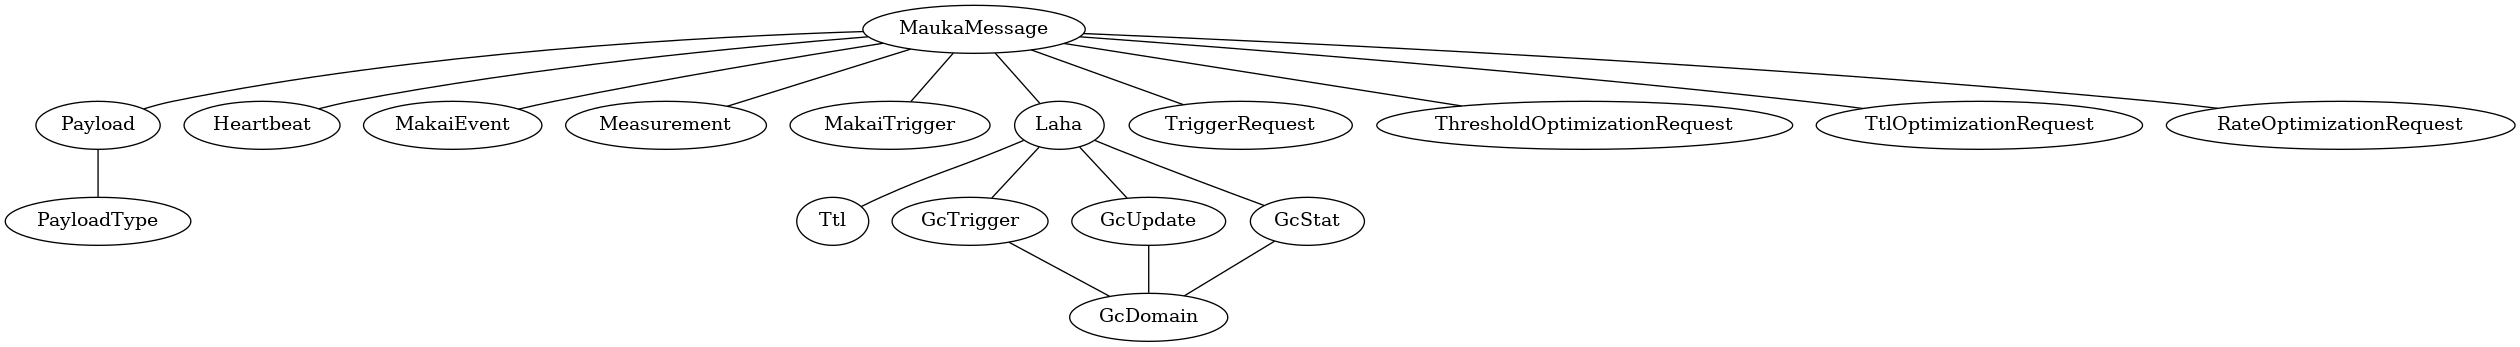
\includegraphics[width=\linewidth]{figures/mauka_messages.png}
	\caption{OPQ Mauka Communications Protocol Summary}
	\label{fig:mauka_messages}
\end{figure}

\subsubsection{Makai Communications Protocol}

Most communication takes place inside of Mauka, however there are several communications channels that occur from Mauka to Makai. These include requesting Event Ids, sending triggers, and sending Box data rate commands. The communications protocols for these actions are described in this section.

Requesting Event Ids from Makai's Event Id Service is performed over a REQ/REP ZMQ socket. Requests from the client should be an empty string. Replies from the host should be a string that only includes the event\_id.

The ``Command" message (Table~\ref{table:Command}) is the base message used for sending commands to Makai and subsequently OPQ Boxes.

\begin{table}[H]
	\centering
	\caption{Command}
	\begin{tabularx}{\textwidth}{lXX}
		\toprule
		\textbf{Field} & \textbf{Type} & \textbf{Description} \\
		\midrule
		seq & uint32 & The command sequence number \\
		box\_id & int32 & The Box Id this command references \\
		timestamp\_ms & uint64 & The timestamp of this command \\
		identity & str & The formatted identity for this command \\
		command & oneof(GetInfoCommand, GetDataCommand, SetMeasurementRateCommand, SendCommandToPlugin) & Command variant \\
		\bottomrule
	\end{tabularx}
	\label{table:Command}
\end{table}

The ``GetDataCommand" message (Table~\ref{table:GetDataCommand}) is sent with a ``Command" message when Mauka wants to trigger Boxes for data.

\begin{table}[H]
    \centering
    \caption{GetDataCommand}
    \begin{tabularx}{\textwidth}{llX}
        \toprule
        \textbf{Field} & \textbf{Type} & \textbf{Description} \\
        \midrule
        start\_ms & uint64 & The start timestamp of the data request. \\
        end\_ms & uint64 & The end timestamp of the data request. \\
        wait & bool & If set, the Box will wait to send data if timestamps are in the future. \\
        \bottomrule
    \end{tabularx}
    \label{table:GetDataCommand}
\end{table}

The ``SetMeasurementRateCommand" (Table~\ref{table:SetMeasurementRateCommand}) message is sent with a ``Command" message when Mauka wants to modify the Measurement rate of OPQ Boxes.

\begin{table}[H]
	\centering
	\caption{SetMeasurementRateCommand}
	\begin{tabularx}{\textwidth}{llX}
		\toprule
		\textbf{Field} & \textbf{Type} & \textbf{Description} \\
		\midrule
		measurement\_window\_cycles & uint32 & How many grid cycles to process per Measurement. \\
		\bottomrule
	\end{tabularx}
	\label{table:SetMeasurementRateCommand}
\end{table}

\subsubsection{Plugin Manager}
Plugins within Mauka are managed using a ``Plugin Manager". The Plugin Manager is responsible for starting, loading, unloading, reloading, terminating, and general management of Mauka plugins at runtime.

The Plugin Manager provides a networked command line interface (CLI) which communicates with the Plugin Manager's ZeroMQ endpoint which is utilized for sending commands and receiving responses to and from the Plugin Manager from any networked device. The CLI uses synchronous request/reply semantics where the client requests a message to the Plugin Manager and the Plugin Manager responds with a response.

The plugin manager can also be used as a library from within Mauka itself accessing the same functionality that is provided by the networked CLI. This functionality is used to initialize the set of plugins that are set to start when Mauka first starts.

Table~\ref{table:PluginManager} commands can be issued from a networked CLI client to interact with the Plugin Manager.

It is important to note some distinctions between the commands. Loading a plugin means loading a plugin from disk into memory where unloading means removing the plugin from memory. Enabling a plugins means that the plugin is loaded and enabled for running. Disabling a plugin means that the plugin is still loaded, but not enabled for running. Starting a plugin means to start a new process for a loaded and enabled plugin where stopping a plugin means to stop a current process and return it to an enabled and loaded state. Killing a plugin uses the OS to send a SIGKILL signal to the process for when its misbehaving and not stopping cleanly on its own.

\begin{table}[H]
	\centering
	\caption{Plugin Manager CLI Reference}
	\begin{tabularx}{\textwidth}{llX}
		\toprule
		\textbf{Command} & \textbf{Arguments} & \textbf{Description} \\
		\midrule
		completions & & Returns a list of completions for auto-complete. \\
		disable-plugin & Plugin name & Disables the named plugin. \\
		enable-plugin & Plugin name & Enables the named plugin. \\
		help & & Displays the help text. \\
		kill-plugin & Plugin name & Kills the named plugin. \\
		load-config & Configuration path & Reloads the configuration from file. \\
		load-plugin & Plugin name & Loads (or reloads) a plugin from disk. \\
		list-plugins & & Lists all loaded plugins. \\
		start-plugin & Plugin name & Starts the named plugin. \\
		stop-plugin & Plugin name & Stops the named plugin. \\
		stop-all-plugins & & Stops all running plugins. \\
		restart-plugin & & Restarts the named plugin. \\
		unload-plugin & Plugin name & Unloads the named plugin. \\
		\bottomrule
	\end{tabularx}
	\label{table:PluginManager}
\end{table}

\subsubsection{Mauka Configuration}
Mauka is highly configurable and it loads various static and dynamic configurations. Static configurations, or configurations that are loaded when Mauka starts are provided by a JSON file. Dynamic configurations related to TTL and garbage collection are stored in the MongoDB and are discussed in detail in Section~\ref{sec:gc_plugin}.

\subsubsection{Mauka Data Models}
Mauka works directly with the following data models: Measurements, Trends, Events, BoxEvents, Incidents, and Phenomena. The data models for these collections are described in this sections.

The Measurements collection contains Instantaneous Measurements produced by Makai. The data model for Measurements is described in Table~\ref{table:Measurement}.

\begin{table}[H]
	\centering
	\caption{Measurement Data Model}
	\begin{tabularx}{\textwidth}{llX}
		\toprule
		\textbf{Field} & \textbf{Type} & \textbf{Description} \\
		\midrule
		box\_id & str & OPQ Box Id \\
		timestamp\_ms & int & Timestamp of the Measurement in milliseconds \\
		expire\_at & int & The timestamp in seconds that this document should be garbage collected \\
		frequency & float & The instantaneous frequency Measurement in Hz \\
		voltage & float & The instantaneous voltage Measurement \\
		thd & float & The instantaneous THD Measurement as a percentage \\
		\bottomrule
	\end{tabularx}
	\label{table:Measurements}
\end{table}

The Trends collection provides summary statistics of frequency, voltage, and THD over a configurable time window. The data model for the Trends collection is given in Table~\ref{table:Trends}.

\begin{table}[H]
	\centering
	\caption{Trend Data Model}
	\begin{tabularx}{\textwidth}{XlX}
		\toprule
		\textbf{Field} & \textbf{Type} & \textbf{Description} \\
		\midrule
		min\_(thd, frequency, voltage) & float & Minimum values for THD, frequency, and voltage \\
		max\_(thd, frequency, voltage) & float & Maximum values for THD, frequency, and voltage \\
		average\_(thd, frequency, voltage) & float & Mean values for THD, frequency, and voltage \\
		box\_id & str & OPQ Box Id \\
		timestamp\_ms & int & Timestamp of end of Trend in milliseconds \\
		location & str & Location slug from the location that this Trend originated from \\
		expire\_at & int & Timestamp in seconds that this document should expire after \\
		\bottomrule
	\end{tabularx}
	\label{table:Trends}
\end{table}

The Events collection contains metadata that map a Makai triggered Event to a list of box\_events which points to raw data for each Box that was requested raw data for that Event. The Event data model is described in Table~\ref{table:Events}.

\begin{table}[H]
	\centering
	\caption{Event Data Model}
	\begin{tabularx}{\textwidth}{llX}
		\toprule
		\textbf{Field} & \textbf{Type} & \textbf{Description} \\
		\midrule
		event\_id & int & Id of the Event generated \\
		description & str & Description of the Event \\
		boxes\_triggered & [str] & A list of box\_ids that were triggered from this Event \\
		boxes\_received & [str] & A list of box\_ids that data was received from \\
		target\_event\_start\_timestamp\_ms & int & Start of the Event \\
		target\_event\_end\_timestamp\_ms & int & End of the Event \\
		expire\_at & int & Timestamp that this document should expire after \\
		\bottomrule
	\end{tabularx}
	\label{table:Events}
\end{table}

The box\_events data model is described in Table~\ref{table:BoxEvents}.

\begin{table}[H]
    \centering
    \caption{BoxEvent Data Model}
    \begin{tabularx}{\textwidth}{llX}
        \toprule
        \textbf{Field} & \textbf{Type} & \textbf{Description} \\
        \midrule
        event\_id & int & ID of the Event this box\_event refers to \\
        box\_id & str & ID of the OPQ Box that sent data for this Event \\
        event\_start\_timestamp\_ms & int & Timestamp of the start of the Event for this Box \\
        event\_end\_timestamp\_ms & int & Timestamp of the end of the Event for this Box \\
        data\_fs\_filename & str & Reference to the waveform stored in gridfs \\
        location & str & Location slug of where this Box sent data from \\
        \bottomrule
    \end{tabularx}
    \label{table:BoxEvents}
\end{table}

The Incidents collection keeps track of Incidents as defined by Laha. This collections includes metadata for classification and other contextual information relating to power Incident. The Incident collection data model is described in Table~\ref{table:Incidents}.

\begin{table}[H]
	\centering
	\caption{Incident Data Model}
	\begin{tabularx}{\textwidth}{llX}
		\toprule
		\textbf{Field} & \textbf{Type} & \textbf{Description} \\
		\midrule
		incident\_id & int & ID of the Incident \\
		event\_id & int & ID of the Event this Incident references \\
		box\_id & str & ID of the OPQ Box that this Incident references \\
		start\_timestamp\_ms & int & Start of this Incident \\
		end\_timestamp\_ms & int & End of this Incident \\
		location & str & Location slug of where this Incident originated from \\
		measurement\_type & str & A description of the Measurements used in this Incident \\
		deviation\_from\_nominal & float & The maximum deviation from nominal for the provided measurement\_type \\
		measurements & [Measurement] & List of Measurements stored in this Incident \\
		gridfs\_filename & str & Location in gridfs that the waveform for this Incident is stored \\
		ieee\_duration & str & An IEEE1159 duration \\
		annotations & [str] & A list of annotations added to this Incident \\
		metadata & object & Metadata associated with this Incident \\
		expire\_at & int & This Incident should expire after this timestamp \\
		\bottomrule
	\end{tabularx}
	\label{table:Incidents}
\end{table}

The ``ground\_truth" stores samples collected from the UH installed power meters. This collection is used to compare Measurements and Trends from OPQ Boxes to the ground truth measured by the UH meters. Each ground truth document consists of meter name, the feature stored, and descriptive statistics for that feature. The ``ground\_truth" data model is described in Table~\ref{table:ground_truth}.

\begin{table}[H]
	\centering
	\caption{Ground Truth Data Model}
	\begin{tabularx}{\textwidth}{llX}
		\toprule
		\textbf{Field} & \textbf{Type} & \textbf{Description} \\
		\midrule
		meter-name & str & Name of the meter this sample is from. \\
		sample-type & str & Name of the feature present in this sample. \\
		ts-s & int & The timestamp of this sample in seconds. \\
		min & float & The minimum value of this feature over the time window. \\
		max & float & The maximum value of this feature over the time window. \\
		avg & float & The average value of this feature over the time window. \\
		stddev & float & The standard deviation of values over the time window. \\
		\bottomrule
	\end{tabularx}
	\label{table:ground_truth}
\end{table}

The ``laha\_config" collection contains dynamic configuration options that Phenomena can alter. The collection is mainly used for defining the default TTL of collections that Mauka manages. The ``laha\_config" data model is described in Table~\ref{table:laha_config}.

\begin{table}[H]
	\centering
	\caption{Laha Config Data Model}
	\begin{tabularx}{\textwidth}{llX}
		\toprule
		\textbf{Field} & \textbf{Type} & \textbf{Description} \\
		\midrule
		box\_samples & int & Default TTL of Box samples. \\
		Measurements & int & Default TTL Measurements. \\
		Trends & int & Default TTL Trends. \\
		Events & int & Default TTL Events and box\_events. \\
		Incidents & int & Default TTL Incidents. \\
		\bottomrule
	\end{tabularx}
	\label{table:laha_config}
\end{table}

The ``laha\_stats" collection contains system statistics that measure various performance metrics in relation to Laha's optimizations. The full details of the ``laha\_stats" collection are provided in Section~\ref{lbl:SystemStatsPlugin}.

The ``makai\_config" collection contains default and Box override thresholds used by Makai's threshold triggering plugin. These items can be dynamically modified by the ``ThresholdOptimizationPlugin" (Section~\ref{subsubsec:threshold-optimization-pugin}).

\begin{table}[H]
	\centering
	\caption{Makai Config Data Model}
	\begin{tabularx}{\textwidth}{XlX}
		\toprule
		\textbf{Field} & \textbf{Type} & \textbf{Description} \\
		\midrule
		default\_ref\_f & f64 & Default reference frequency \\
		default\_ref\_v & f64 & Default reference voltage \\
		default\_threshold\_percent\_f\_low & f64 & Default frequency percent low threshold \\
		default\_threshold\_percent\_f\_high & f64 & Default frequency percent high threshold \\
		default\_threshold\_percent\_v\_low & f64 & Default voltage percent low threshold \\
		default\_threshold\_percent\_v\_high & f64 & Default voltage percent high threshold \\
		default\_threshold\_percent\_thd\_high & f64 & Default THD percent high threshold \\
		triggering\_overrides & [MakaiConfigOverride] & List of Box specific overrides \\
		\bottomrule
	\end{tabularx}
	\label{table:makai_config}
\end{table}

\begin{table}[H]
	\centering
	\caption{Makai Config Override Data Model}
	\begin{tabularx}{\textwidth}{XlX}
		\toprule
		\textbf{Field} & \textbf{Type} & \textbf{Description} \\
		\midrule
		box\_id & str & Override Box Id \\
		ref\_f & f64 & Override reference frequency \\
		ref\_v & f64 & Override reference voltage \\
		threshold\_percent\_f\_low & f64 & Override frequency percent low threshold \\
		threshold\_percent\_f\_high & f64 & Override frequency percent high threshold \\
		threshold\_percent\_v\_low & f64 & Override voltage percent low threshold \\
		threshold\_percent\_v\_high & f64 & Override voltage percent high threshold \\
		threshold\_percent\_thd\_high & f64 & Override THD percent high threshold \\
		\bottomrule
	\end{tabularx}
	\label{table:makai_config_override}
\end{table}

The ``phenomena" collection contains metadata relating to Phenomena produced by Mauka. The data model for Phenomena is provided in Table~\ref{table:phenomena_data_model}.

\begin{table}[H]
	\centering
	\caption{Phenomena Data Model}
	\begin{tabularx}{\textwidth}{XlX}
		\toprule
		\textbf{Field} & \textbf{Type} & \textbf{Description} \\
		\midrule
		phenomena\_id & int & Id of the Phenomena \\
		related\_incident\_ids & [int] & List of related Incident Ids. \\
		related\_event\_ids & [int] & List of related Event Ids. \\
		affected\_opq\_boxes & [str] & List of OPQ Boxes affected by this Phenomena. \\
		start\_ts\_ms & int & Start time of the Phenomena. \\
		end\_ts\_ms & int & End time of the Phenomena. \\
		phenomena\_type: Object & Metadata and parameters for specific Phenomena types. \\
		\bottomrule
	\end{tabularx}
	\label{table:phenomena_data_model}
\end{table}

\subsubsection{PQ Plugins}\label{ssec:pq_plugins}
Mauka's functionality is provided by plugins that perform analysis, data management, health, and system tuning. Communication within Mauka is performed using type safe message passing. This section describes in detail how each plugin functions and also documents each plugins inputs and outputs.

\paragraph{BasePlugin.}
All plugins derive from a single ``BasePlugin". The BasePlugin provides primitives for running plugins as separate processes, serialization and deserialization of type safe messages, communication over ZeroMQ, metrics collection, MongoDB communication, debugging, and plugin health.

To support running plugins as separate processes, the BasePlugin provides a ``run\_plugin" method that instantiates the new plugin inside of a new process. The BasePlugin provides signal handlers to catch SIGKILL and SIGINT signals from the system and cleanly exit the plugin process. The BasePlugin also contains an ``exit\_event" which can be set from other processes to inform the plugin to exit cleanly. This is used when Mauka is cleanly shutdown or when a plugin is stopped from the PluginManager.

When a BasePlugin process is started, the plugin creates a timer that runs at a configurable interval. When the timer fires, a heartbeat for the subclassing plugin is produced. This provides health information for each plugin within Mauka.

The BasePlugin provides automatic serialization and deserialization of protobuf Mauka messages produced and received for each plugin.

The BasePlugin provides functionality for automatically serializing and deserializing waveform from MongoDB's gridfs.

The BasePlugin provides ZMQ endpoints for producing and consuming messages to and from topics for each plugin. The BasePlugin ensures that all accesses to brokers are handled atomically with multiprocessing locks.

The BasePlugin keeps track of the number of messages sent and received for each plugin as well as the number of bytes sent and received for each plugin. This information is included in each plugin's heartbeat and later uses for calculating and storing metrics for each plugin.

The BasePlugin uses the configurable debugging interface to selective display debug messages for a plugin. Debug messages are only displayed for plugins that are configured to display debug messages in Mauka's configuration.

The BasePlugin provides a MongoDB client for each plugin for reading and writing to the database.

\paragraph{MakaiEventPlugin.} The ``MakaiEventPlugin" is responsible for reading Events newly created by Makai into Mauka. It performs feature extraction on the raw Event data streams and forwards those features (or the raw data) to subscribing plugins. This allows Mauka to perform the important feature extraction once, and reuse those features in multiple plugins.

The MakaiEventPlugin subscribes to messages from with the subject ``MakaiEventMessage". These messages are described in Table~\ref{table:MakaiEvent}. When a message is received, the plugin waits a configurable amount of time to ensure that Makai has finished writing data to the database. Once the data is in the database, the plugin loads the raw data and performs feature extraction.

The raw waveform from the OPQ Box is serialized into a Payload (Table~\ref{table:Payload}) with PayloadType (Table~\ref{table:PayloadType}) ``ADC\_SAMPLES" and produced to the topic ``AdcSamples".

The raw voltage is calculated by dividing each sample of the raw waveform by the calibration constant loaded from the database that is set for each device. The raw voltage  is serialized into a Payload (Table~\ref{table:Payload}) with PayloadType (Table~\ref{table:PayloadType}) ``VOLTAGE\_RAW" and produced to the topic ``RawVoltage".

$V_{rms}$ is the peak-to-peak voltage over a configurable time window. By default, Mauka uses a time window of one electrical cycle at 60$Hz$ which works out to be $1/60$ seconds. $V_{rms}$ is calculated by moving a running window over the raw voltage waveform. The computation of $V_{rms}$ for each window with $n$ samples is given by Equation~\ref{equation:Vrms}. The RMS voltage is serialized into a Payload (Table~\ref{table:Payload}) with PayloadType (Table~\ref{table:PayloadType}) ``VOLTAGE\_RMS\_WINDOWED" and produced to the topic ``RmsWindowedVoltage".

\begin{equation}
\label{equation:Vrms}
	V_{RMS} = \sqrt{\frac{\sum_{i=0}^{n} n_{i}^2}{n}}
\end{equation}

Windowed frequency is the frequency calculated for a configurable time window. By default, Mauka uses a time window of one electrical cycle at 60$Hz$ which works out to be $1/60$ seconds. The frequency is calculated by first smoothing the raw voltage waveform by applying a $4^{th}$ order Butterworth filter to the waveform with a cutoff frequency of 500$Hz$ and a down sampling rate of 2. Then, a window is moved across the smoothed signal and the frequency is calculated for each window by performing a least squares regression and fitting a sinusoide. The windowed frequency is serialized into a Payload (Table~\ref{table:Payload}) with PayloadType (Table~\ref{table:PayloadType}) ``FREQUENCY\_WINDOWED" and produced to the topic ``WindowedFrequency".

When new Events are received by the MakaiEventPlugin, a GcUpdate (Table~\ref{table:GcUpdate}) message is produced informing the LahaGcPlugin that all ``measurements" and ``trends" stored by Makai should receive a TTL of the newly created Event.

\paragraph{FrequencyVariationPlugin.}
The ``FrequencyVariationPlugin" is used to classify generic frequency sags, swells, and interruptions as defined by the IEEE1159 standard\cite{IEEE:2018:1159D3}. Both duration and deviation from nominal are used to perform these classifications. Duration classifications include frequency deviations that last for less than 50 ns, between 50 ns to 1 ms, and 1 ms to 50 ms. Classifications for deviations from nominal are performed for values that are up to 40\% deviation nominal. The plugin subscribes to messages from the ``WindowedFrequency" topic which includes a payload of frequency features over one electrical cycle.

When a message is received, the plugin uses configurable thresholds to find frequency fluctuations within the windowed frequency streams. The plugin is able to classify frequency swells, frequency interruptions, and frequency sags. When a new frequency variation is detected, a frequency Incident is created and a GC\_UPDATE message is sent to the LahaGcPlugin to update the TTL of all Measurements, Trends, and Events that belong to this new Incident.

\paragraph{IEEE1159VoltagePlugin.}
The ``IEEE1159VoltagePlugin" is a plugin that is able to classify voltage Incidents in accordance to the IEEE1159 standard\cite{IEEE:2018:1159D3}. In general, this standard classifies voltage disturbances by duration and by magnitude. voltage durations are classified from 0.5 to 30 cycles, 30 cycles to 3 seconds, 3 seconds to a minute, and greater than 1 minute. voltage deviations are classified in both the sag and swell directions as a percentage from nominal. Sags are generally classified between 10\% and 90\% of nominal while swells are generally classified from 110\% to 180\% of nominal.  The plugin subscribes to messages from the ``RmsWindowedVoltage" topic which includes payloads of $V_{RMS}$ features over a window of one electrical cycle.

This plugin is capable of classifying voltage sags, swells, and interruptions as defined by the standard. The plugin works by identifying sags, swells, and interruptions and determining the duration of those Events. If the duration or delta is large enough, a voltage Incident is created and a GC\_UPDATE message is sent to the LahaGcPlugin asking it to update the TTL for all Measurements, Trends, and Events that belong to this new Incident.

\paragraph{AnnotationPlugin.}

The ``AnnotationPlugin" is responsible for creating and storing Annotation Phenomena within Mauka. The Annotation Plugin subscribes to ``AnnotationRequest" messages which include a start and end timestamp, a list of affected OPQ Boxes, a list of related Event Ids, and a list of related Incident Ids.

When an AnnotationRequest is received, the request is parsed and the data is stored and structured in the database using the Phenomena data model.

At the time of writing, AnnotationRequests are generated manually and inserted into the system using the MockPlugin which allows any type of message to be constructed and produced to any other plugins. Annotations are created when users of the OPQ network can correctly identify the source of a PQ signal.

\paragraph{BoxOptimizationPlugin.}

The ``BoxOptimizationPlugin" is responsible for sending and receiving typed messages to and from OPQ Boxes from OPQ Mauka. This plugin is capable of requesting the state of each OPQ Box (e.g. uptime, Measurement rate, security keys, etc). This plugin is also capable of adjusting the state of individual OPQ Boxes by changing things such as the Measurement and Trend rate or the sampling rate that the Box is sampling at.

This plugin subscribes to two topics, ``BoxOptimizationRequest" and "BoxMeasurementRateRequest". When a BoxOptimizationRateRequest is received by the plugin, the plugin queries the Boxes specified in the request for data about their state. Because this is completely asynchronous, a separate thread is spawned to receive the response from the Boxes. When a response is received in the spawned thread, the response is produced to any plugins that are subscribed to the response and interested in the result.

When a BoxMeasurementRateRequest is received, the plugin sends a message to all Boxes marked in the request along with new Measurement and Trends rates (in cycles) that the Box should adjust to use. It is important to note that Makai caches these values for a maximum of one minute. Therefore, to adjust the Measurement or Trend rate at time $T$, the adjustment should really take place at $T - 60$ so that the new value is utilized by the Box and not the cached value over the duration of change. Once the rates have been changed, the Box sends an asynchronous response back to Mauka which is received in a separately spawned thread, a MeasurementRateResponse is created and forwarded to interested plugins.

\paragraph{FuturePhenomenaPlugin.}

The ``FuturePhenomenaPlugin" is responsible for creating Future or Predictive Phenomena. These Phenomena are used to predict Events and Incidents that may occur in the future. This plugin does not subscribe to any messages, but instead utilizes timers to perform its work. By default, this plugin runs every 10 minutes.

When the plugin runs, it loads any active Periodic Phenomena found in the database. If Periodic Phenomena are found, this plugin extrapolates possible Events and Incidents by first examining the timestamps of previous periods and then extrapolating into the future using the mean period and the standard deviation. For each timestamp in the periodic phenomena, the mean period is added. If the resulting timestamp is in the future, a Future Phenomena is created using the time range of the future timestamp $\pm$ standard deviation of the Periodic Phenomena.

When a Future Phenomena is created, a timers are started in a separate thread signifying the start and end timestamps of the Future Phenomena. When the first timer runs, messages are sent to the BoxOptimizationPlugin and the ThresholdOptimizationPlugin instructing Event thresholds to be set lower and Box Measurement rates to be set higher. This increases the chance of seeing an Event over the predicted time window. When the second timer runs, these values are reset to their default values. Thus, the plugin increases fidelity and decreases thresholds over the period of a Future Phenomena.

This plugin also tracks the number of Events and Incidents that were identified utilizing Future Phenomena. If a Future Phenomena does not detect any Events or Incidents, I say that the Phenomena is not realized. If it does detect Events or Incidents, I say that the plugin is realized.

\paragraph{ITICPlugin.}
The ``ITICPlugin" analyzes $V_{rms}$ to determine where it falls within the ITIC curve\cite{thallam2000power}. The ITIC curve is a power acceptability curve that plots time on the x-axis and $V_{rms}$ on the y-axis. The ITIC curve is displayed in Figure~\ref{fig:IticCurve}.

\begin{figure}
	\centering
	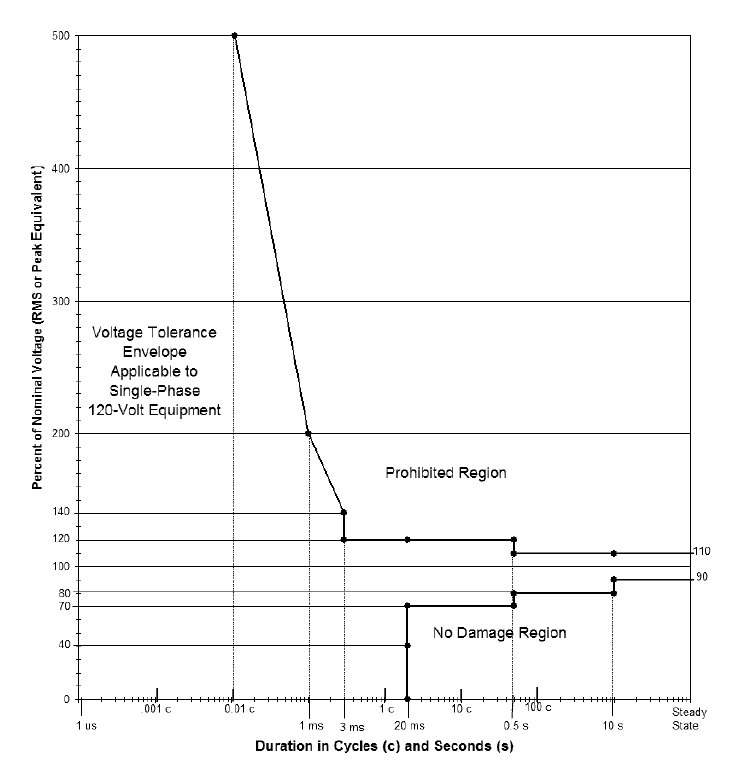
\includegraphics[width=\linewidth]{figures/itic.png}
	\caption{ITIC Curve}
	\label{fig:IticCurve}
\end{figure}

The purpose of the curve is to provide a tolerance envelope for single-phase 120V equipment. Meaning it defines the sustained voltage tolerance at different time durations. The curve defines three regions. The first region is ``No Interruption" and generally includes all voltages with very short sustained durations. All power Events within this region have no noticeable effect on power equipment. The second region, the ``No Damage Region", occurs during voltage sags for extended periods of time. Power Events in this region may cause equipment interruptions, but it will not damage the equipment. The final region, the``Prohibited Region", is caused by sustained voltage swells and may cause damage to power equipment.

The ITICPlugin subscribes to the ``RmsWindowedVoltage" topic. When it receives a message, it extracts the windowed voltage features and uses a segmentation algorithm to split the features into segments of sustained voltage. The segmentation algorithm is rather naive and described below.

Given an array of values $A$, the length of the array $len(A)$, and a segmentation threshold $t$:
\begin{enumerate}
	\item Find all $i$ where $A_i - A_{i-1} > t$
	\item Segments over $A$, ($SA$), are then defined as [$SA_{0..i_0}, SA_{i_0..i_1}, \dots, SA_{i_n..len(A)}$]
\end{enumerate}

Once the segments are defined, we calculate the duration of each segment. We know that each sample in the $V_{rms}$ features represents one electrical cycle at 60$Hz$. Thus, to find the duration of a segment in milliseconds we can simply divide the number of cycles by the number of cycles in milliseconds. Thus, $duration\_ms = \frac{cycles}{0.06}$. The plugin also calculates the mean $V_{rms}$ for each segment. Once we have a duration and mean $V_{rms}$ for each segment, we can plot it on the ITIC curve and get a region classification.

In order to plot the value on the curve, the curve is first constructed as a set of polygons representing each ITIC region. Each polygon is represented by an array of points (see Appendix~\ref{appendix:Itic}). Once the polygons are constructed, matplotlib's point-in-polygon algorithm is used to determine which ITIC region a point of $(duration\_ms, V_{rms})$ falls within. If a region of ``No Interruption" or ``Prohibited" is returned, then a new ITIC Incident is created and stored to the database.

If a new Incident is created, a message is sent to the LahaGcPlugin informing the plugin to update the TTL of all Measurements, Trends, and Events that belong to the Incident.

\paragraph{LahaGcPlugin.}\label{sec:gc_plugin}
Mauka provides custom garbage collection (GC) for identifying and removing ``uninteresting" data. This fulfills one of Laha's claims that it is able to manage data storage pressure while increasing the signal-to-noise ratio within the data set.

In order for Mauka to know when items should be GCed, all elements stored in the database are assigned a TTL. A default TTL is assigned when the element is first created, but can be updated later by Mauka plugins depending on if that data is deemed ``interesting".

Data within Laha is continually refined with context and by importance in Laha and by extension, OPQ does the same. As data is deemed interesting by Mauka, it is moved upward through the Laha hierarchy by Laha Actors. In the case of Mauka, this means moving raw data and features from OPQ Boxes into Mauka. When Mauka identifies interesting features of this data, it is moved into Events. Interesting enough Events are moved into Incidents, and collections of Incidents are moved into Phenomena. Whenever data is moved upwards, that data receives the TTL of its parent, and thus, will live for as long as its parent does.

Originally, Mauka relied on MongoDB's Time-to-Live (TTL) semantics for expiring and deleting uninteresting data. This did not provide the flexibility needed for Mauka's refined garbage collection needs. For example, MongoDB's TTL could only be applied to entire collections and not dynamically to individual elements in the collection. MongoDB's TTL was also difficult to update dynamically based on the state of the system. Because we want to assign TTLs dynamically (as interesting data is moved upwards) we required a more robust solution to TTL and GC management.

Default TTLs are dynamically stored in the Mongo database under the ``laha\_config" collection and the ``ttls" key. Since the TTLs are stored in the database, they can be updated and tuned by Mauka's Phenomena.

Table~\ref{table:DefaultTtls} displays the default TTL in seconds for each OPQ collection.

\begin{table}[H]
    \centering
    \caption{Default TTLs for OPQ Collections}
    \begin{tabularx}{\textwidth}{XX}
        \toprule
        \textbf{Collection} & \textbf{Default TTL seconds} \\
        \midrule
        box\_samples & 900 \\
        Measurements & 86400 \\
        Trends & 1209600 \\
        Events & 2620800 \\
        Incidents & 31449600 \\
        Phenomena & 62899200 \\
        \bottomrule
    \end{tabularx}
    \label{table:DefaultTtls}
\end{table}

As each item is saved to the database, it is assigned with a default TTL as described in Table~\ref{table:DefaultTtls}. If the item that was assigned to the database is later deemed important by Mauka and is referenced by a parent item, it receives the TTL of the parent item allowing that data to live as long as the parent does. If the parent item is a Phenomena, then all data relating to that Phenomena (from all levels are the hierarchy) will live forever. The process of updating

The Mauka plugin ``LahaGcPlugin" is responsible for GC and TTL management. Each plugin in Mauka produces a heartbeat at a predefined interval. GC within the LahaGcPlugin takes place every time the plugin produces a heartbeat.

Other than heartbeats, it is also possible to trigger the GC by sending a message to the GC plugin with a list of collections that should be GC\@.

When the LahaGcPlugin receives a ``GcTrigger" message, it extracts from the message the list of collections that should be GCed. Heartbeats will trigger all collections to be GCed.

The Measurements and Trends collections perform GC by simply removing from the database all Measurements and Trends that have a TTL that is older than the current date and time.

Events in OPQ are spread out over three collections: Events, box\_events, and gridfs files. Events contain metadata about an Event which includes information about all Boxes that sent data in response to that Event. Each Box that sent data for an Event will spawn a box\_event document which includes information relating to a Box for a specific Event. Further, each box\_event document points to where the raw data is stored in MongoDB using the gridfs data layer provided by the database.

In order to GC Events, first all Events with a TTL less than the current date and time are identified. From the Events, we look up the corresponding box\_events. From each box\_event, we look up corresponding raw data in gridfs. First the gridfs data is removed, then the box\_events are removed, and finally the Events themselves are removed.

To GC Incidents, a similar algorithm is provided. First, Incidents with a TTL less than the current date and time are identified. From these identified Incidents, Mauka looks up and removes the corresponding data in gridfs. Finally, the Incidents are removed.

Phenomena, being the top of the hierarchy are GCed the least since it provides the most context for optimizing the DSN. Phenomena are only GCed when they are shown to be incorrect or are otherwise unused over the period of a year. Thus, Phenomena take the same default TTL as Incidents. Phenomena differ from Incidents in that every time a Phenomena is referenced by the DSN, it is TTL is renewed for another year from the last use date. Similarly to other collections, when a Phenomena's TTL is updated, all collections that the Phenomena references will also have their TTL updated.

Metrics for GC (i.e.\ the number of items removed per collection) are stored providing insights to data management and effectiveness.

The Mauka GC plugin does not manage raw data on OPQ Boxes. Instead, OPQ Boxes manage their own internal data buffer with a TTL that can be configured on the Box.

Dynamically updating TTLs is also performed by the LahaGcPlugin. The LahaGcPlugin listens for specific ``Ttl" messages that contain the source item that the TTL is being updated for. Then all child elements of the source element also have their TTLs updated. TTLs are updated in the following manner.

When new Events are created, the TTL of Measurements and Trends that coincide with that Event receive the TTL of the Event. When Incidents are created, the Events, Trends, and Measurements associated with that Incident receive the TTL of the Incident. When Phenomena are created, the TTLs of Incidents, Events, Trends, and Measurements are assigned the TTL of the Phenomena (which is infinite).

\paragraph{MockPlugin.}
The ``MockPlugin" is a special plugin that can be instantiated at run time and sends and receives messages to configurable topics. This plugin is useful for debugging and rerunning (or running new) analysis over old data. As an example, let us say a new plugin Foo is designed. We want to run historical data through Foo. To do that, the MockPlugin can be configured to read the database for all old Events, and then construct a message to Foo so that Foo runs its analysis over those Events.

\paragraph{OutagePlugin.}
The ``OutagePlugin" classifies power outages. Since no real power data is produced during an outage, this plugin only subscribes to its own heartbeats. When a heartbeat is received, the outage plugin looks up in the database all OPQ Boxes that are marked ``down" by OPQ Health and not marked as ``unplugged" in the database. This plugin keeps track of current outages so that if an OPQ Box is already in an outage state a new outage Incident is not created on each subsequent heartbeat.

When outage Incidents are created, TTL update messages are not sent because there is no data during the time period of an outage to adjust the TTL for.

\paragraph{PeriodicityPlugin.}

The ``Periodicity Plugin" is responsible for detecting periodic signals in power data. This plugin does not subscribe to any messages, but instead runs off of a configurable timer. The plugin is set to run by default once an hour and every hour it scrapes the last 24 hours worth of data and attempts to find periods in the Measurements over that duration.

For each feature in the Measurement and Trend data (e.g. frequency, voltage, and THD), the Periodicity plugin first removes the DC offset from the data by subtracting the mean. Next, the plugin filters the signal using a 4th order high-pass filter to filter out noise. The plugin then performs autocorrelation on the signal followed by finding the peaks of the autocorrelation. The mean distance between the peaks of the autocorrelation ($\mu$) provides the period of the signal.

The plugin only classifies data as periodic if at least 3 peaks were found and the standard deviation of the period ($\sigma$) is less than 600 seconds (10 minutes). Once a positive identification has been made, peak detection is performed on the original signal using the $\mu$ and $\sigma$ parameters found from autocorrelation to parameterize the peak detection algorithm. The peaks of the original signal represent the times and deviations from nominal for that feature.

Once the plugin has the timestamps and deviations from nominal of the periodic signal of interest, the plugin can group Measurements, Trends, Events, and Incidents that were created during the periodic signals together as part of the Periodic Phenomena.

As an example, Figure~\ref{fig:periodic_example} shows periodic voltage sags observed at Box 1021.

\begin{figure}[h]
	\centering
	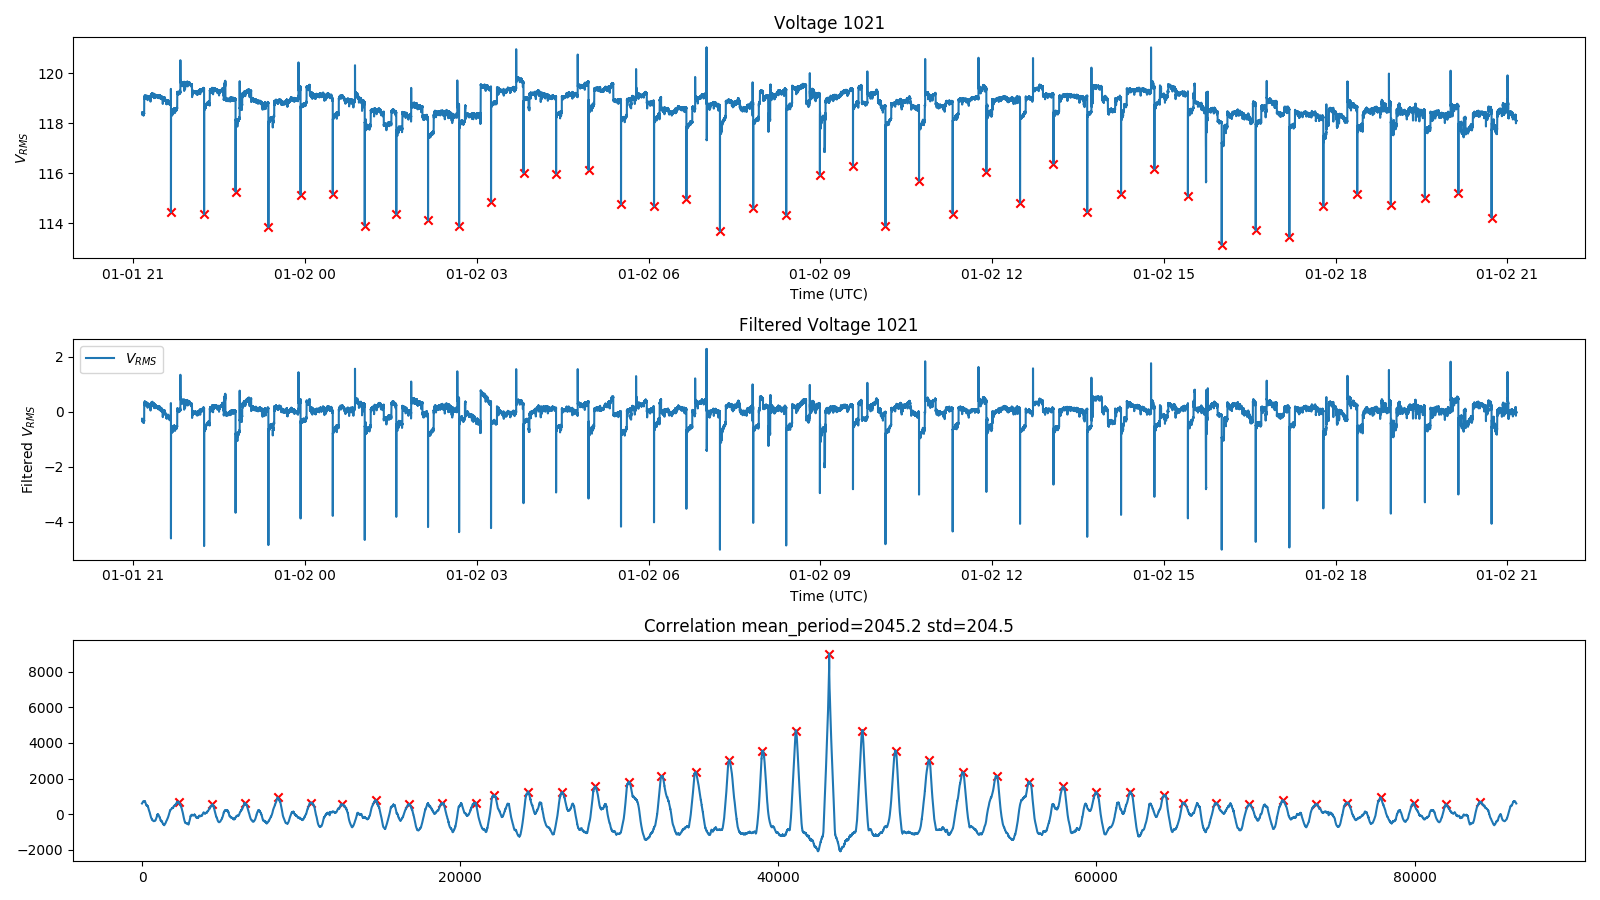
\includegraphics[width=\linewidth]{figures/periodic_example.png}
	\caption{Periodic Phenomena Example}
	\label{fig:periodic_example}
\end{figure}

The top panel shows the original signal. The middle panel shows the filtered signal. The bottom panel shows the results of autocorrelation. In this example, we can see how the filtered data was autocorrelated and then peak detection was performed on the autocorrelated signal to find the mean period in seconds ($\mu$ = 2045.2 seconds) and the standard deviation in seconds ($\sigma$ = 204.5 seconds). This is shown in the third panel. The periodicity metrics are then used to find all peaks in the original data that are at least $mu$ - $sigma$ seconds apart. These peaks are shown in the first panel.

The Periodicity Plugin also performs several pieces of housekeeping. It is possible that a Periodic Phenomena already exists in the database for the same sensor and feature set. If that is the case, the original Periodic Phenomena is updated if the newly identified period contains more autocorrelation peaks and a smaller standard deviation than the one that is already stored. In the Event that the plugin stops seeing periodic data for Phenomena that already exists, the plugin sets the Phenomena as ``no longer active" signaling that the Periodic Phenomena is no longer observing the periodic signal of interest. The plugin also identifies Events and Incidents that have taken place during the reported periodic signals.

\paragraph{SimilarityPlugin.}
The ``SimilarityPlugin" attempts to find groupings of Incidents that are similar. This plugin uses a similarity distance metric computed from the normalized duration of the Incident and the normalized deviation from nominal of the Incident.

This plugin runs on a configurable timer (default of 24 hours). It loads all Incidents and groups them by Incident type. K-means clustering is utilized to find groupings of related Incidents, with empirically found $k$ values for each Incident type. For example, $k=8$ for frequency Incidents provides decent characterization of Incidents by both duration and deviation from nominal.

When clusters are found, they are saved to the database as Similarity Phenomena. Each similarity Phenomena maintains metadata about the Incidents contained within the Phenomena as well as metadata describing the mean deviation from nominal and mean duration.

Optionally, this plugin can be configured to act on Incidents as they arrive. Using an initial set of clusters found, the newly arrived Incident can be inserted into the correct cluster. Parameters describing ``non-interesting" cluster (e.g. less than 1 second and closer to nominal for frequency Incident) can be provided to this plugin. If a new Incident is classified into a non-interesting cluster, the Phenomena is updated to include this Incident, but the Incident is not saved to disk, providing data savings and reducing the total number of Incidents so that only more interesting Incidents remain.

\paragraph{PrintPlugin.}
The ``PrintPlugin" is a special plugin that is mainly used for debugging. It subscribes to all topics and simply prints the contents of the message to STDOUT. This is useful in development or when bringing up a new Mauka system to ensure that the communications infrastructure is in place. It can also be enabled at runtime from the Mauka CLI to debug all communication channels for all plugins.

\paragraph{SemiF47Plugin.}
The ``SemiF47" plugin is another plugin like the IticPlugin that plots voltage and duration against a power acceptability curve. In this case, the standard used is the SemiF47 standard\cite{semif47}. Rather than using a point-in-polygon approach, this plugin reads the $V_{RMS}$ features sequentially and uses a state machine to keep track of the current classification. This plugin only classifies values as a ``violation" or as ``nominal".

The SemiF47 curve is displayed in Figure~\ref{fig:SemiF47Curve}.

\begin{figure}
	\centering
	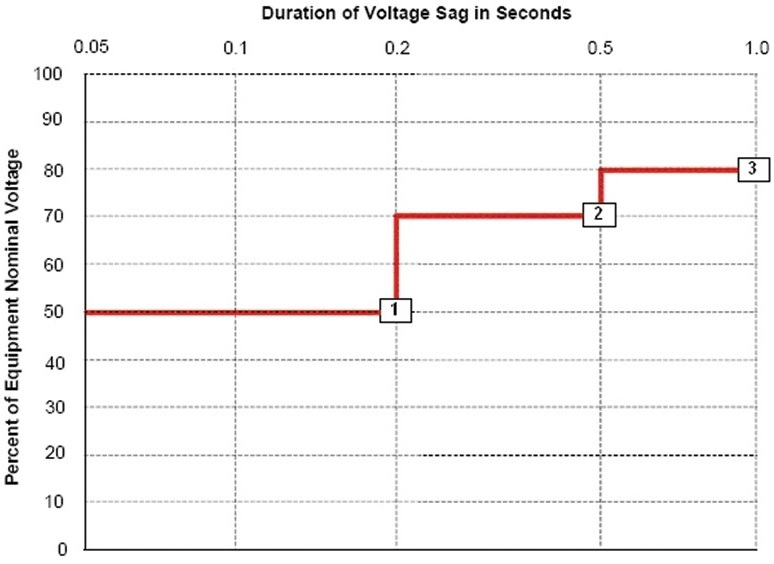
\includegraphics[width=0.6\linewidth]{figures/semif47.jpg}
	\caption{SemiF47 Curve}
	\label{fig:SemiF47Curve}
\end{figure}

SemiF47 is described in Table~\ref{fig:SemiF47Table}.

\begin{figure}
	\centering
	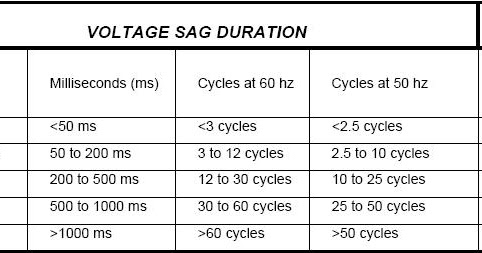
\includegraphics[width=0.6\linewidth]{figures/semif47_table.jpg}
	\caption{SemiF47 Table}
	\label{fig:SemiF47Table}
\end{figure}


\paragraph{StatusPlugin.}
Mauka provides a health endpoint that can be queried by OPQ Health to determine the health status of Mauka. The health status is saved to a database by Health and shown in OPQ View.

The Mauka plugin ``StatusPlugin" is responsible for obtaining and providing the status of the OPQ Mauka service. The plugin subscribes to heartbeats sent at configurable intervals from all other plugins including itself. When the plugin receives a heartbeat, it updates its internal state which includes a mapping of all plugins, their state, and the last time that plugin sent a heartbeat.

The plugin provides a configurable HTTP endpoint which is queried by OPQ Health. The plugin extracts the internal health state and serializes the state as JSON using the protocol described in Table~\ref{table:HealthProtocol}. This protocol is standardized for health collection across all OPQ services.

\begin{table}[H]
	\centering
	\caption{Mauka HealthProtocol}
	\begin{tabularx}{\textwidth}{llX}
		\toprule
		\textbf{Field} & \textbf{Type} & \textbf{Description} \\
		\midrule
		name & string & Name of the service \\
		ok & bool & Whether the entire service is ok or not \\
		timestamp & int & The timestamp of when the health request was received \\
		subcomponents & [HealthProtocol] & Health protocol for each plugin \\
		\bottomrule
	\end{tabularx}
	\label{table:HealthProtocol}
\end{table}

\paragraph{SystemStatsPlugin.}\label{lbl:SystemStatsPlugin}
Mauka collects and stores many different types of performance metrics in order to demonstrate the efficacy of Laha as implemented in Mauka. The metrics are collected by the ``SystemStatsPlugin" Mauka plugin and are stored in the MongoDB collection `laha\_metrics`.

The metrics are conditioned and displayed in OPQ View for easy analysis. It is possible to select a start and end date/time to configure the time window of metrics displayed in view. Examples of Mauka's metrics displayed in OPQ View are shown in Figure~\ref{fig:Metrics1}, Figure~\ref{fig:Metrics2}, and Figure~\ref{fig:Metrics3}.

\begin{figure}
	\centering
	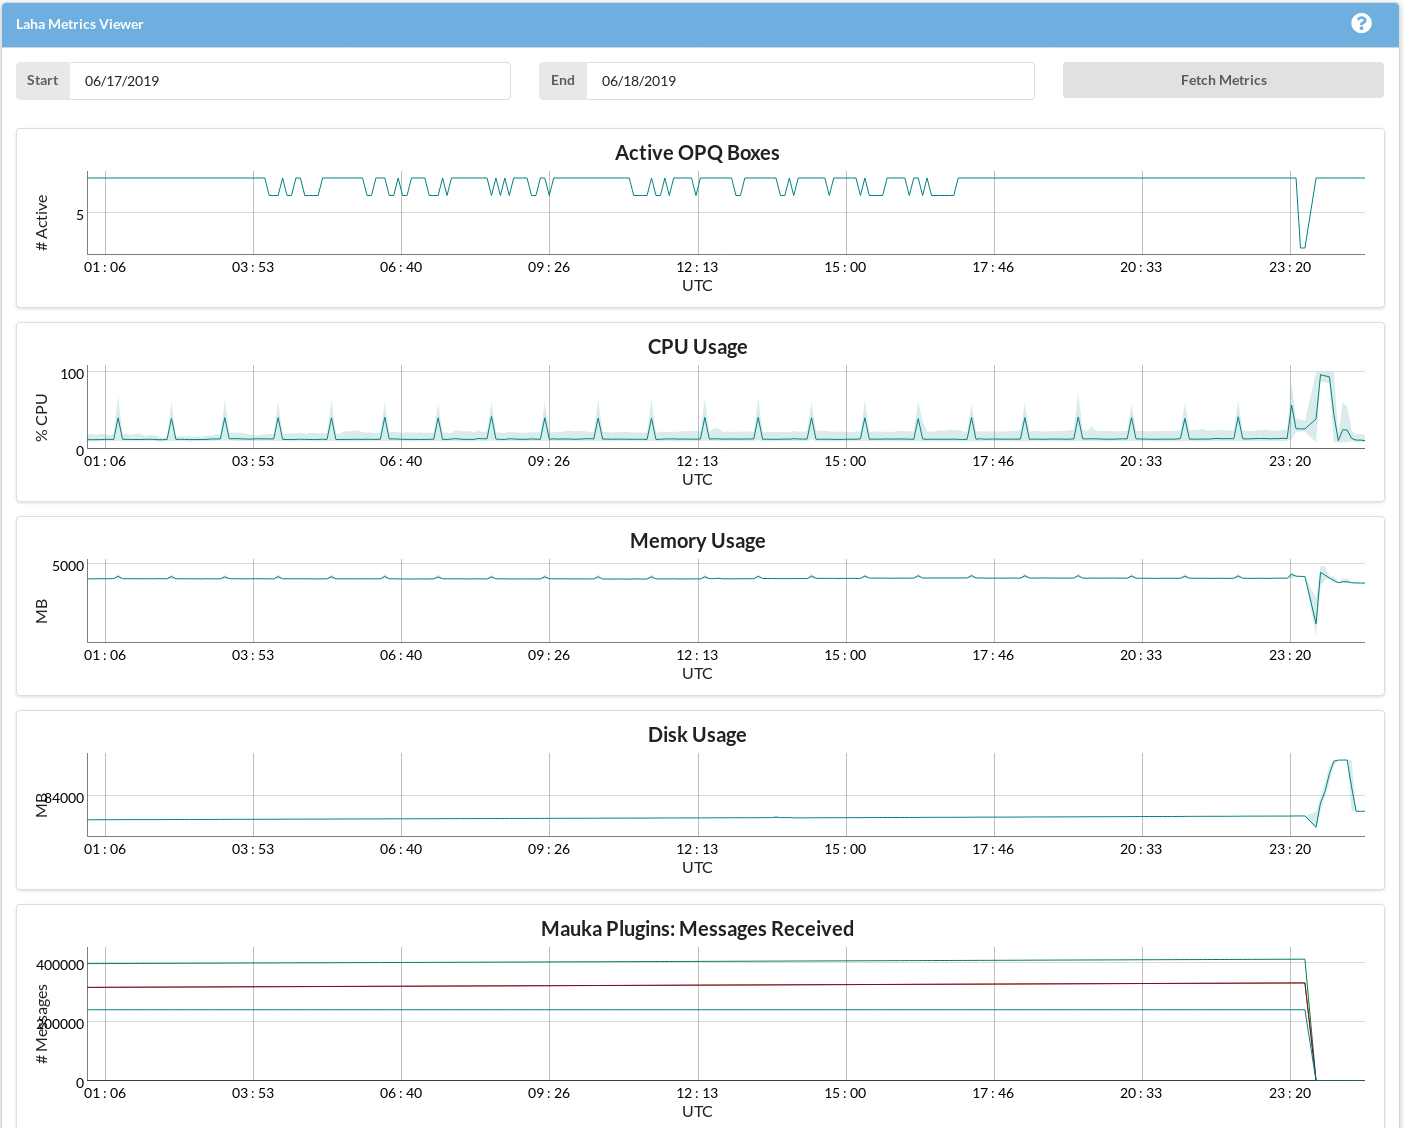
\includegraphics[width=\linewidth]{figures/metrics_1.png}
	\caption{OPQ Mauka Metrics I}
	\label{fig:Metrics1}
\end{figure}

\begin{figure}
	\centering
	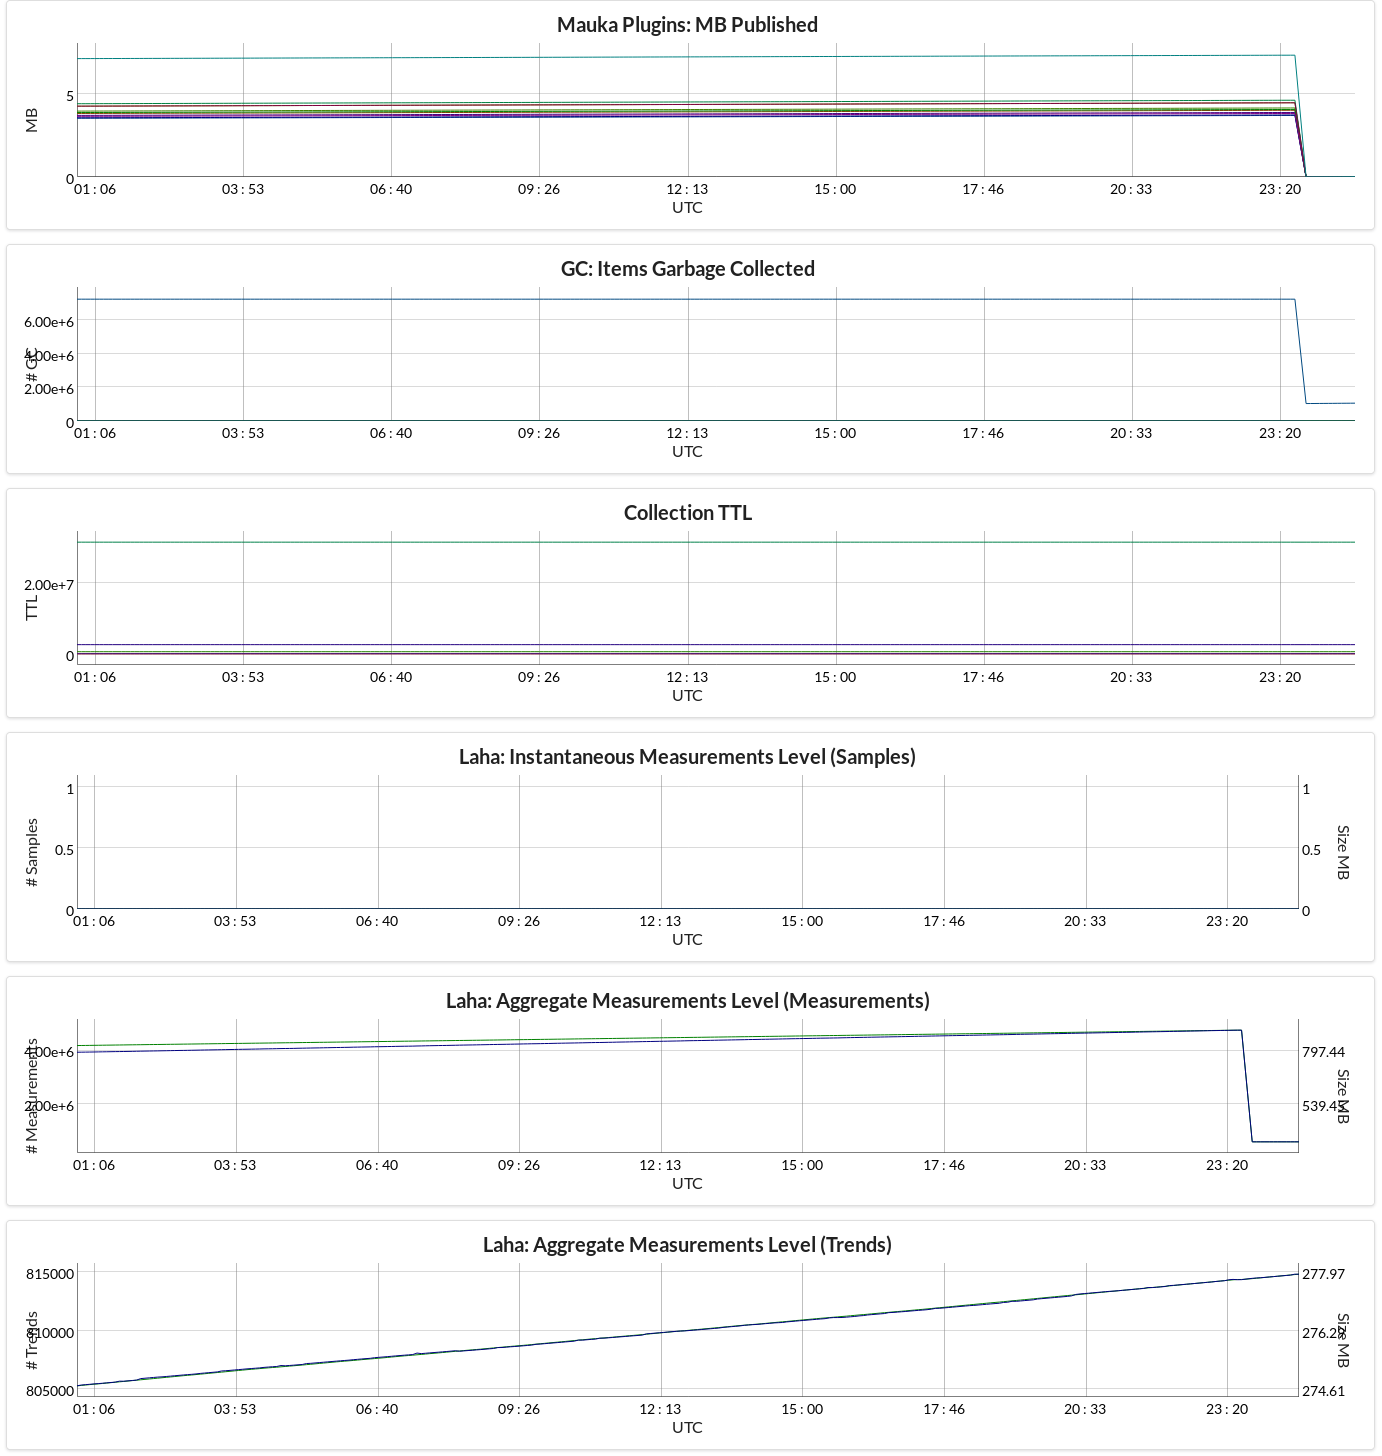
\includegraphics[width=\linewidth]{figures/metrics_2.png}
	\caption{OPQ Mauka Metrics II}
	\label{fig:Metrics2}
\end{figure}

\begin{figure}
	\centering
	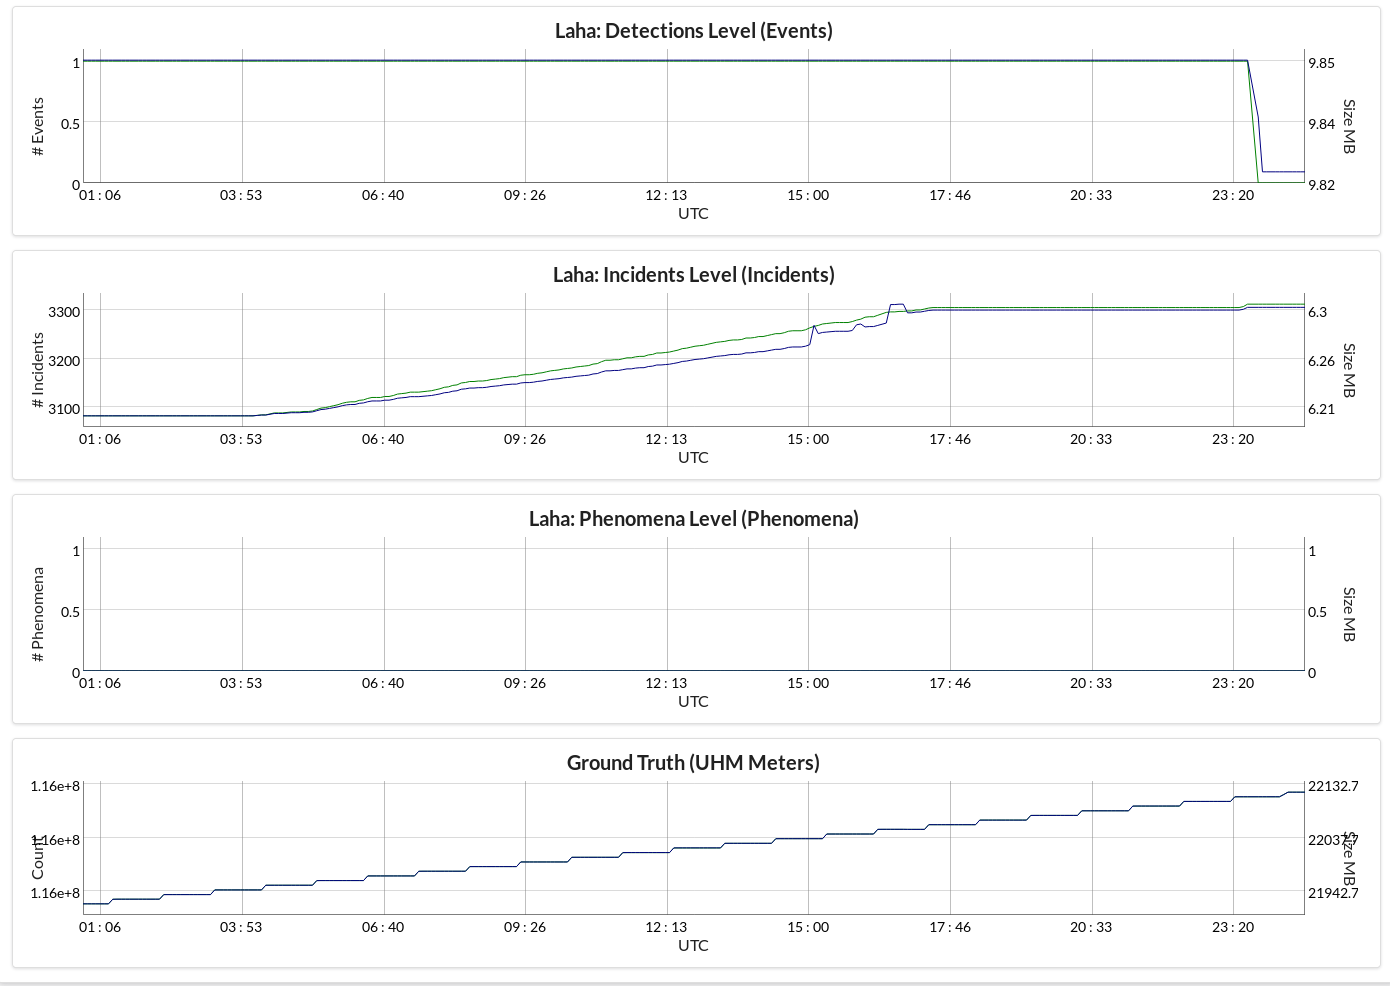
\includegraphics[width=\linewidth]{figures/metrics_3.png}
	\caption{OPQ Mauka Metrics III}
	\label{fig:Metrics3}
\end{figure}

The types of metrics collected include plugin statistics, system statistics, and Laha statistics which provide metrics on data usage and TTL for data stored within each Laha level as well as garbage collection statistics for each level of the hierarchy.

Metrics are collected at a configurable interval. System statistics such as CPU usage, memory usage, and disk usage are sampled once every 10 seconds. Once every 5 minutes, all metrics are saved to disk. The system statistic metrics which are sampled more frequently are rolled into a 5 minute metric only storing min, max, mean, variance, count, and start and end timestamp.

Mauka metrics consist of nested documents. The following Table describes each of the documents stored in the metrics collection.

The base document shown in Table~\ref{table:Metrics} contains links to all of the high level metrics that Mauka collects. This includes metrics for plugins, system statistics, Laha metrics, and ground truth.

\begin{table}[H]
	\centering
	\caption{Mauka Metrics}
	\begin{tabularx}{\textwidth}{llX}
		\toprule
		\textbf{Metric} & \textbf{Type} & \textbf{Description} \\
		\midrule
		plugin\_stats & [PluginStat] & List of metrics for each plugin. \\
		system\_stats & [SystemStat] & System statistics for CPU, memory, and disk usage. \\
		laha\_stats & [LahaStat] & Statistics on count, size, and TTL for each collection. \\
		ground\_truth\_count & int & Count of ground truth documents. \\
		ground\_truth\_size\_bytes & int & Size of ground truth in bytes. \\
		\bottomrule
	\end{tabularx}
	\label{table:Metrics}
\end{table}

Plugin metrics are described in Table~\ref{table:MetricsPluginStat} and mainly records the plugin name and the number and size of messages received and produced for each plugin.

\begin{table}[H]
	\centering
	\caption{PluginStat}
	\begin{tabularx}{\textwidth}{llX}
		\toprule
		\textbf{Metric} & \textbf{Type} & \textbf{Description} \\
		\midrule
		messages\_received & int & The number of messages the plugin has received. \\
		messages\_published & int & The number of messages the plugin has published. \\
		bytes\_received & int & The number of bytes the plugin has received. \\
		bytes\_published & int & The number of bytes the plugin has published. \\
		\bottomrule
	\end{tabularx}
	\label{table:MetricsPluginStat}
\end{table}

System metrics as shown in Table~\ref{table:MetricsSystemStat} use descriptive statistics over a time window to collect the minimum, maximum, mean, variance, and count of memory, disk, and CPU usage.

\begin{table}[H]
	\centering
	\caption{SystemStat}
	\begin{tabularx}{\textwidth}{llX}
		\toprule
		\textbf{Metric} & \textbf{Type} & \textbf{Description} \\
		\midrule
		min & float & Minimum value over time window. \\
		max & float & Maximum value over time window. \\
		mean & float & Mean value over time window. \\
		var & float & Variance of values over time window. \\
		cnt & int & The number of items sampled over time window. \\
		start\_timestamp\_s & int & Start timestamp of time window. \\
		end\_timestamp\_s & int & End timestamp of time window. \\
		\bottomrule
	\end{tabularx}
	\label{table:MetricsSystemStat}
\end{table}


The Laha metrics described in Table~\ref{table:MetricsLaha} store metrics relating to the TTL, size, and count of Laha collections.

\begin{table}[H]
	\centering
	\caption{LahaStat}
	\begin{tabularx}{\textwidth}{llX}
		\toprule
		\textbf{Metric} & \textbf{Type} & \textbf{Description} \\
		\midrule
		ttl & int & Default TTL for a Laha level. \\
		count & int & Number of items in a Laha level. \\
		size\_bytes & int & Size of a Laha level in bytes. \\
		\bottomrule
	\end{tabularx}
	\label{table:MetricsLaha}
\end{table}

\paragraph{ThdPlugin.}
The ``ThdPlugin" classifies abnormal amounts of total harmonic distortion (THD) in a power waveform. THD is a measure of amount of noise in the frequency at multiples of 60Hz. The ThdPlugin subscribes to messages from the ``AdcSamples" topic which include payloads consisting of raw samples from the OPQ Boxes. THD is calculated using a rolling window of one electrical cycle over the waveform. For each window, THD is calculated by Equation~\ref{equation:Thd}.

\begin{equation}
\label{equation:Thd}
	THD_F = \frac{\sqrt{V_2^2 + V_3^2 + V_4^2 + \dots}}{V_1}
\end{equation}

For each continuous set of windows that has THD higher than the configured threshold, a THD Incident is created. If an Incident is created, this plugin sends a GC\_UPDATE message to the LahaGcPlugin informing it that it should update all Measurements, Trends, and Events that belong to the new Incident to match the Incident's TTL\@.


\paragraph{TransientPlugin.}
The ``TransientPlugin" is responsible for classifying frequency transients in power waveforms. The plugin subscribes to messages from the ``RawVoltage" topic which contains a calibrated power waveform payload. The TransientPlugin is capable of classifying impulsive, arcing, oscillatory, and periodic notching transients. A decision tree is utilized to select the most likely transient type and then further analysis is used to perform the actual classification of transients.

Dickens et al\cite{csdl2-19-02} provides more details on the transient classification system.

When a transient is classified a new transient Incident is created. If an Incident is created, this plugin sends a GC\_UPDATE message to the LahaGcPlugin informing it to update the TTLs for all Measurements, Trends, and Events that belong to this new Incident.

\paragraph{TriggerPlugin.}\label{sec:trigger_plugin}
The ``TriggerPlugin" provides Mauka with the functionality to trigger OPQ Boxes itself instead of relying on Makai for triggering. Generally, Mauka is only provided with event\_ids when Makai triggers Boxes based off of their low-fidelity data streams. Mauka then loads the associated Event data from the database, performs cycle level feature extraction, and then forwards those features to analysis plugins for PQ analysis.

This plugin takes advantage of Phenomena in order to find Incidents that may not have passed Makai's triggering thresholds.

This plugin consists of two threads running in a single process. The main thread (or the plugin thread) is responsible for listening for ``TriggerRequest" messages from other plugins and sending trigger requests to Makai's acquisition broker. The second data thread is responsible for listening for data from triggered Boxes routed through Makai.

The only stateful component between a data request and a data response is an identity string which is a specially crafted string that allows Makai to route requests through its services. The format of an identity string is ``[topic]\_[event\_token]\_[uuid]". In Mauka's case, the ``[topic]" is always set to ``mauka", the ``[event\_token]" is a randomly generated v4 UUID (which provides $2^{122}$ bits of collision space), and the ``[uuid]" is the box\_id of the Box being triggered. The issue however is that both threads need to know more than just the identity. For instance, they need to know things like which ``event\_id" and ``incident\_id" a data response belongs to to or which Boxes we are still waiting for a response from.

To accomplish data sharing between the two threads, a thread safe ``TriggerRecords" class was created. This class uses a reentrant lock to lock mappings from ``event\_token" to all of ``event\_id", ``incident\_id", ``timestamp\_ms" (of record insert), and ``triggered\_boxes".  Details of how these mappings are used are provided below.

This plugin listens for ``TriggerRequest" messages from other plugins. When it receives a ``TriggerRequest", it constructs protobuf data commands that Makai can consume. Each data command is for a single Box and includes start and end timestamps as milliseconds since the epoch. Each data command also contains an identity string which determines how the message is routed through Makai's services.

The data commands described in Section~\ref{table:Command} are serialized and sent over a ZMQ PUSH/PULL socket to Makai's acquisition broker. Makai's acquisition broker then goes out to the requested Boxes (if they are available) and requests raw data for the requested time window.

Previously, Makai handled all Event storage. With this plugin, Mauka now has to handle Event storage for Boxes that Mauka has triggered. This includes creating and modifying the Event document metadata, BoxEvent document metadata, and gridfs waveform storage.

Just after the data commands are sent to Makai's acquisition broker, a ZMQ REQ/REP channel is used to query Makai's Event Id service. Makai's Event Id service provides atomic access to the next available Event Id for storage of Events in the Mongo database. Once the next available Event Id is received by Mauka, it is used to create a new Event document in the database with the new Event Id, the Event time window, and a list of triggered Boxes.

Just after the event\_id is received, the plugin updates the thread-safe TriggerMappings class with mappings from the new event\_token to the new event\_id, the incident\_id, the Boxes triggered, and the timestamp of the triggers.

In order to receive data requested from the Boxes, this plugin starts a separate data thread when this plugin starts. The data thread connects to a Makai acquisition broker endpoint over ZMQ using a PUB/SUB channel. The data thread subscribes to all topics that start with ``mauka\_" which will match all identities generated by Mauka and will ignore trigger requests initiated by Makai.

When data is received for a Box in the data thread, the metadata and uncalibrated waveform cycles are extracted from the deserialized message. We also extract event\_id information from the thread-safe TriggerRecords class using the response's event\_token. A ``BoxEvent" document is created in the Mongo database for the newly received data and the waveform is written to gridfs and metadata pointing to the gridfs file is provided in the BoxEvent.

Next, the original Event document is updated to insert the received box\_id into the ``received\_boxes" field.

Then, the received Box Id is removed from the TriggerRecords class since we are no longer waiting on it. If this was the last Box we were waiting on for an associated event, then the trigger record associated with this identity is removed and a message with the new event\_id is sent to the ``MakaiEventPlugin" which then forwards feature extracted data to the rest of the analysis pipeline.

By using the above approach, we ensure that we never request analysis of the data until all triggered Boxes are received for a particular event. However, we can run into the issue of triggered Boxes never returning data for a request. To deal with this issue, the TriggerRecords class timestamps each record that is inserted. If the data receive thread does not receive data from all triggered Boxes within a configurable amount of time (default 1 minute), then the records are removed and an event\_id is sent to the ``MakaiEventPlugin" so that it can process data for all of the Boxes that it did receive.

Data triggered from Mauka is fundamentally different than data triggered from Makai. That is because Boxes triggered from Mauka are always triggered from an associated Incident or Phenomena. If new Incidents are found from this data and they are similar to the original Incident that caused Mauka to trigger, then we have found a global event and possible Phenomena that would not have been observed using Makai's triggering alone. This requires extra semantic information to be passed to the ``MakaiEventPlugin" and other analysis plugins. Data received from Mauka triggers are always forwarded with the associated Incident or Phenomena Id so that the relationships can be tracked and maintained.

\paragraph{ThresholdOptimizationPlugin.}\label{subsubsec:threshold-optimization-pugin}
The ThresholdOptimizationPlugin is responsible for modifying dynamic triggering thresholds within Makai. Makai utilizes two methods for triggering Boxes. One method called ``Napali" was produced by Sergey Negrashov as part of his dissertation research. The Napali trigger uses a windowed statistical model for triggering devices based off of metric distance from standard deviations and means. The second approach to triggering is a threshold trigger which watches frequency, voltage, and THD levels to determine whether they have passed certain thresholds. This plugin works with the second type of triggering, the threshold trigger. Threshold based triggering is described in Section~\ref{subsubsec:dynamic-triggering}.

Thresholds are stored in MongoDB and consist of default thresholds and override thresholds which are thresholds set specifically for individual devices. This plugin can dynamically modify both types of thresholds. The data model for thresholds are presented in Table~\ref{table:makai_config}.

This plugin receives the MaukaMessage variant ``ThresholdOptimizationRequest" (described in Section~\ref{table:ThresholdOptimziationRequest}). When a request is received, the default thresholds can be updated, a single override threshold can be updated, or both can be updated at the same time.

For any default value in the request that is larger than 0, the default threshold value in the database is updated with the new request value. If the request contains an override value larger than 0, this plugin first checks to see an override for that Box already exists in the database. If an override already exists, then the override is updated with the new override values from the request. If the override does not exist, then a new override is created with default values and the override values are updated from the request.

\paragraph{RateOptimizationPlugin.}

The ``RateOptimizationPlugin" is responsible for modifying the send rate of Measurements for specific Boxes. This plugin subscribes to ``RateOptimizationRequest" messages (described in Section~\ref{table:RateOptimizationRequest}) which include a Box Id and requested sample rate for the Measurements collection.

Requests from this plugin are sent from Phenomena when a Phenomena believes that changing the Measurement rate of a Box or Boxes could enhance Mauka's ability to discover signals of interest.

When a request is received, this plugin sends a Makai Command (Section~\ref{table:Command}) to Makai's acquisition broker over a ZMQ socket. The command message includes the Box Id and Measurement sample rate. Makai then handles forwarding the command to the relevant Box which will then change its Measurement rate to match that of the request.

\paragraph{TtlOptimizationPlugin.}\label{subsubsec:ttl-optimization-pugin}

The ``TtlOptimizationPlugin" is responsible for dynamically modifying ``laha\_config" collection TTL values. This plugin subscribes to ``TtlOptimizationRequest" messages (Section~\ref{table:TtlOptimizationRequest}).

When a request is received, the corresponding TTL value in the database is updated to match the requested value.

This plugin only affects TTL values for newly generated Measurements, Trends, Event, Incidents, and Phenomena and will not update the TTL values of documents that are already in the database.

\subsubsection{Debugging OPQ Mauka}
The Mauka system can be configured so that only specified plugins print debug messages. This is accomplished by specifying the names of the plugins which should print debug output in Mauka's configuration file. Without this functionality, parsing through the entirety of Mauka's log output would be a daunting task.

\subsection{OPQ: View}\label{subsec:opq:-view}
OPQ View is a web application that provides visualization, notification, and user management services for data, sensors, and user accounts with the OPQ framework. OPQ View is built using Meteor.js and provides a Reactive view of the underlying data stored in the OPQ database.

A screenshot of OPQ View in action is provided in Figure~\ref{fig:opq-view}.

\begin{figure}
	\centering
	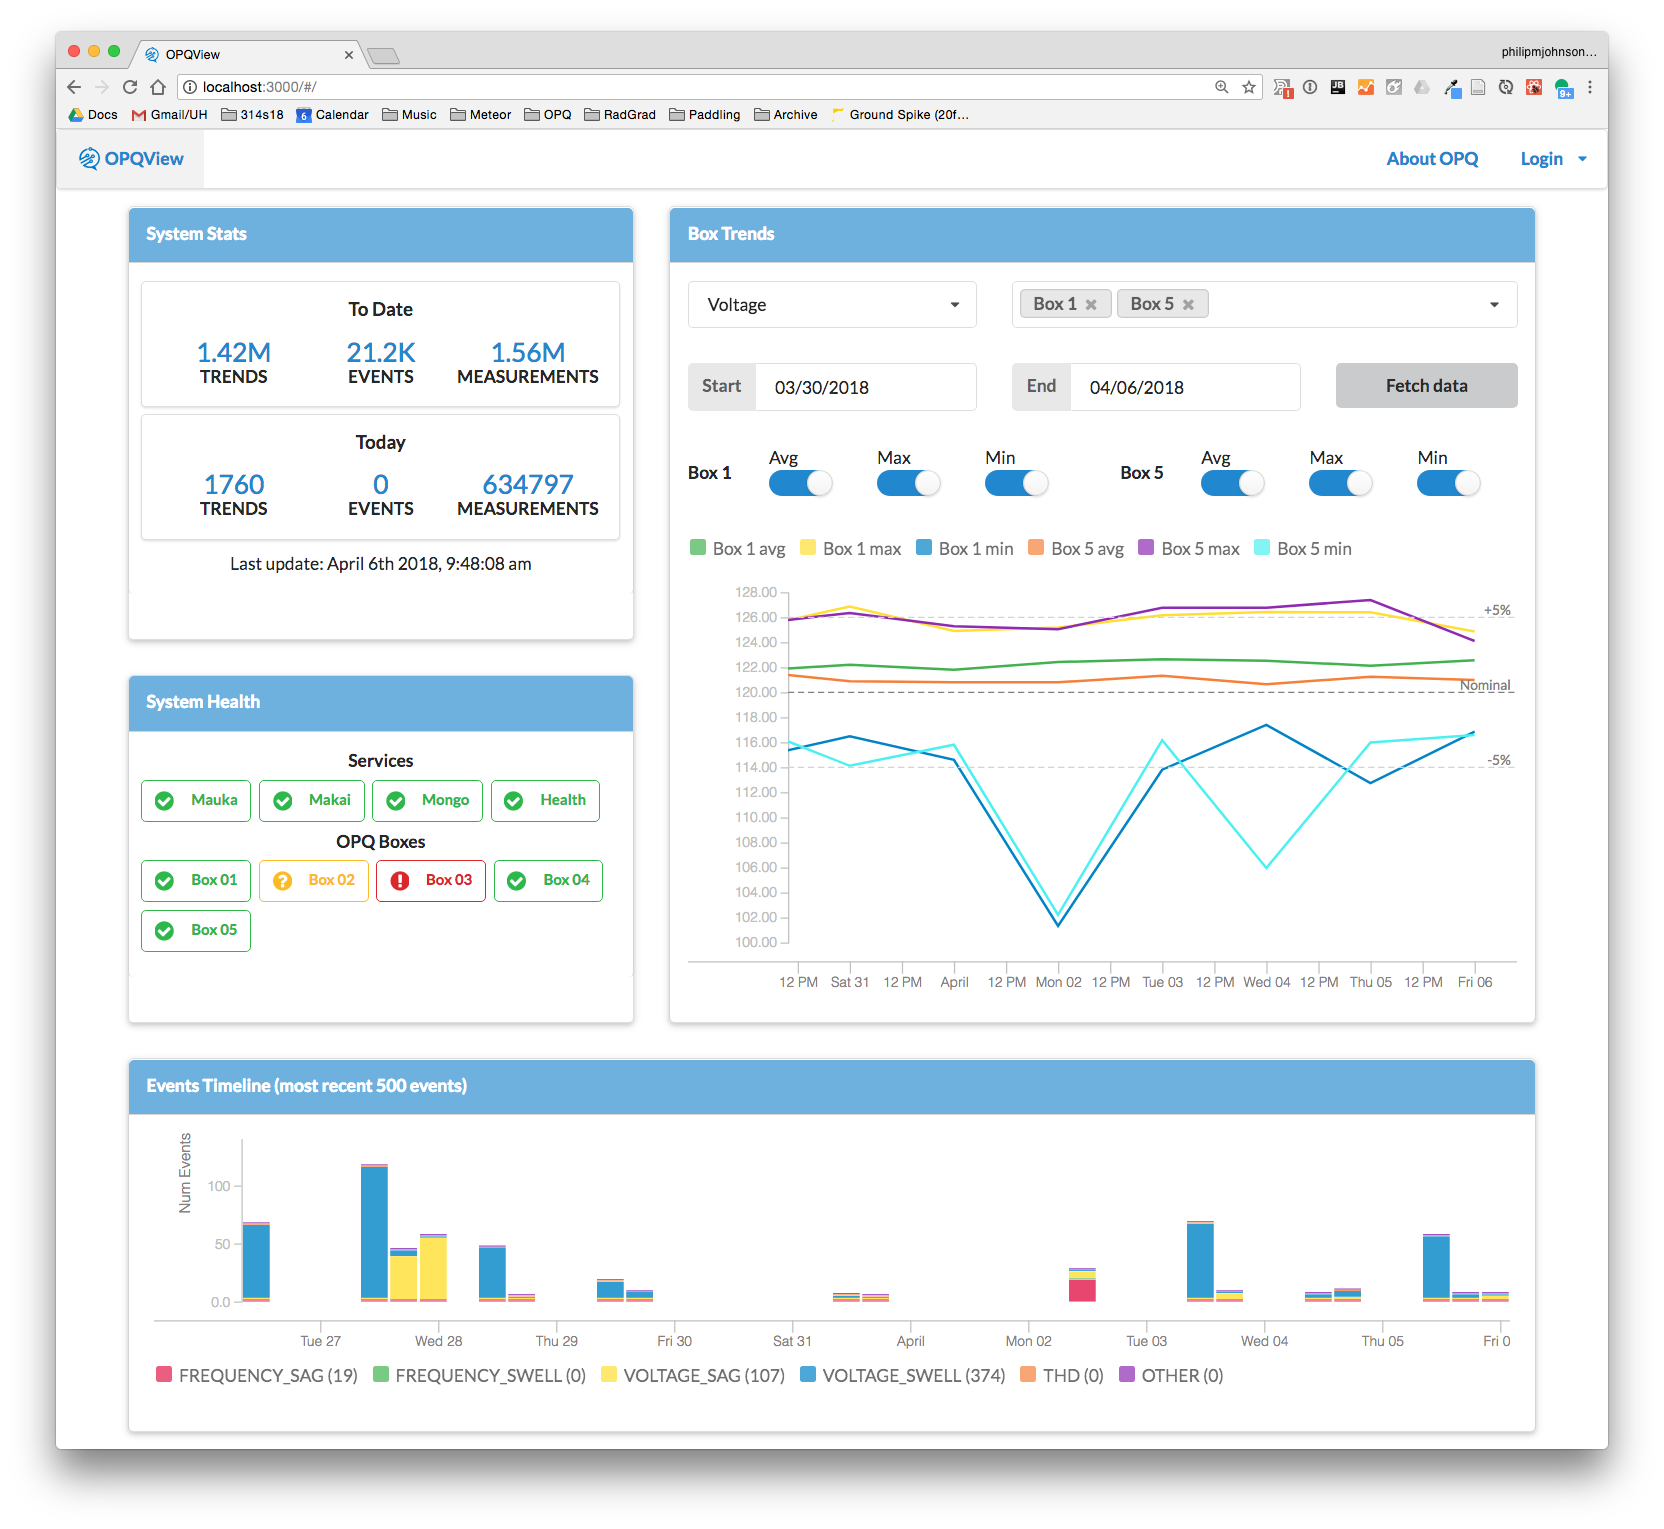
\includegraphics[width=1\linewidth]{figures/opqview-landing-page.png}
	\caption{OPQ View Screenshot}\label{fig:opq-view}
\end{figure}

For the most part, OPQ View serves as a client for displaying PQ information collected and analyzed by the rest of the framework. However, OPQ View provides two components that are directly related to this dissertation.

OPQ View provides the ability to manually define minimum and maximum triggering thresholds for voltage, frequency, and THD used by Makai. Figure~\ref{fig:view_thresholds} shows what this functionality looks like as implemented in View.

\begin{figure}
	\centering
	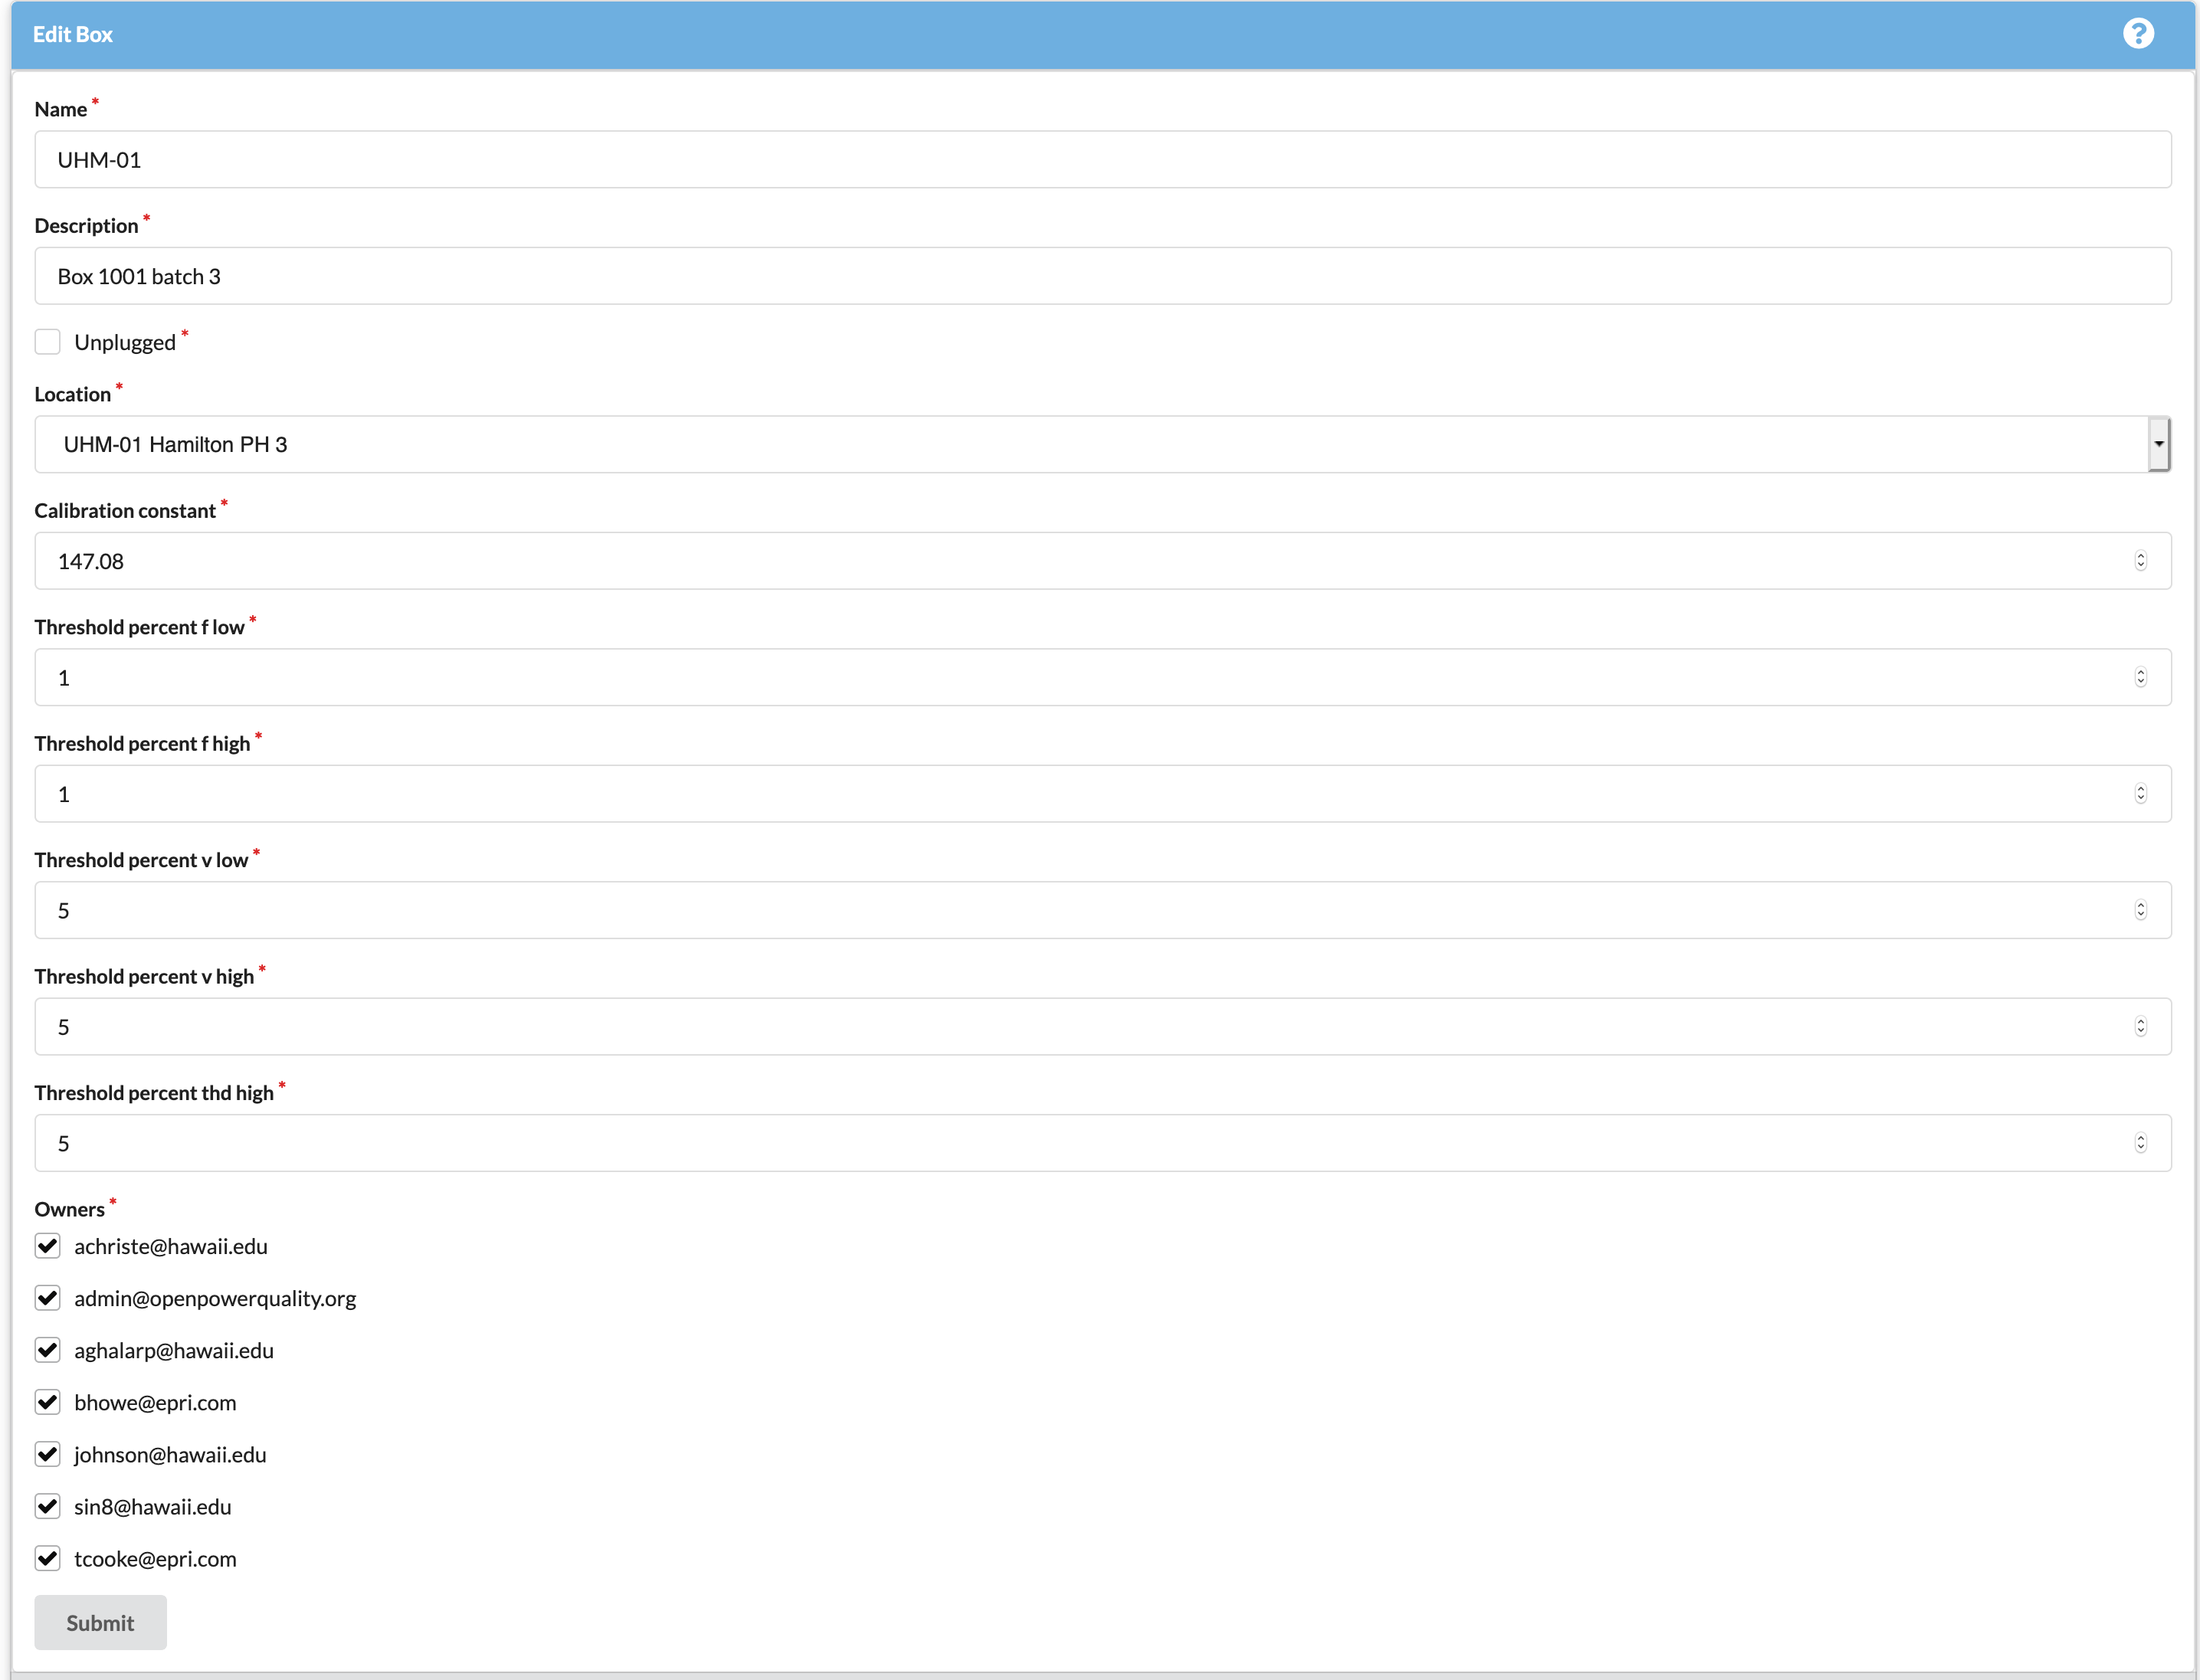
\includegraphics[width=1\linewidth]{figures/view_thresholds.png}
	\caption{OPQ View Threshold Configuration}\label{fig:view_thresholds}
\end{figure}

OPQ View also provides a display for Laha metrics that were collected by Mauka. This is described and shown in Section~\ref{lbl:SystemStatsPlugin}.

\subsection{OPQ: Dockerfication}\label{subsec:opq:-dockerfication}
The OPQ system is made up of many separate services and technology stacks. Each service has its own build process and set of other services that it communicates with. In order to streamline the building and deployment of OPQ services, we implemented a containerized architecture using Docker and Docker Compose. This architecture allows us to track the version of each service and provide the OPQ Cloud system as a monolithic service managed by Docker. This greatly simplifies deployment of not just individual services, but deployment of the entire system as a whole.

Each OPQ service runs in its own Docker container. Each container is configured so that network access is restricted to only the other containers that it is allowed to communicate with. Docker also allows us to manage which ports are open to the outside world for any particular service.

Docker also restricts access to the filesystem. These features combined help to provide a secure environment for the execution of OPQ services.

The Docker architecture that OPQ uses is presented in Figure~\ref{fig:docker_deploy}.

\begin{figure}
	\centering
	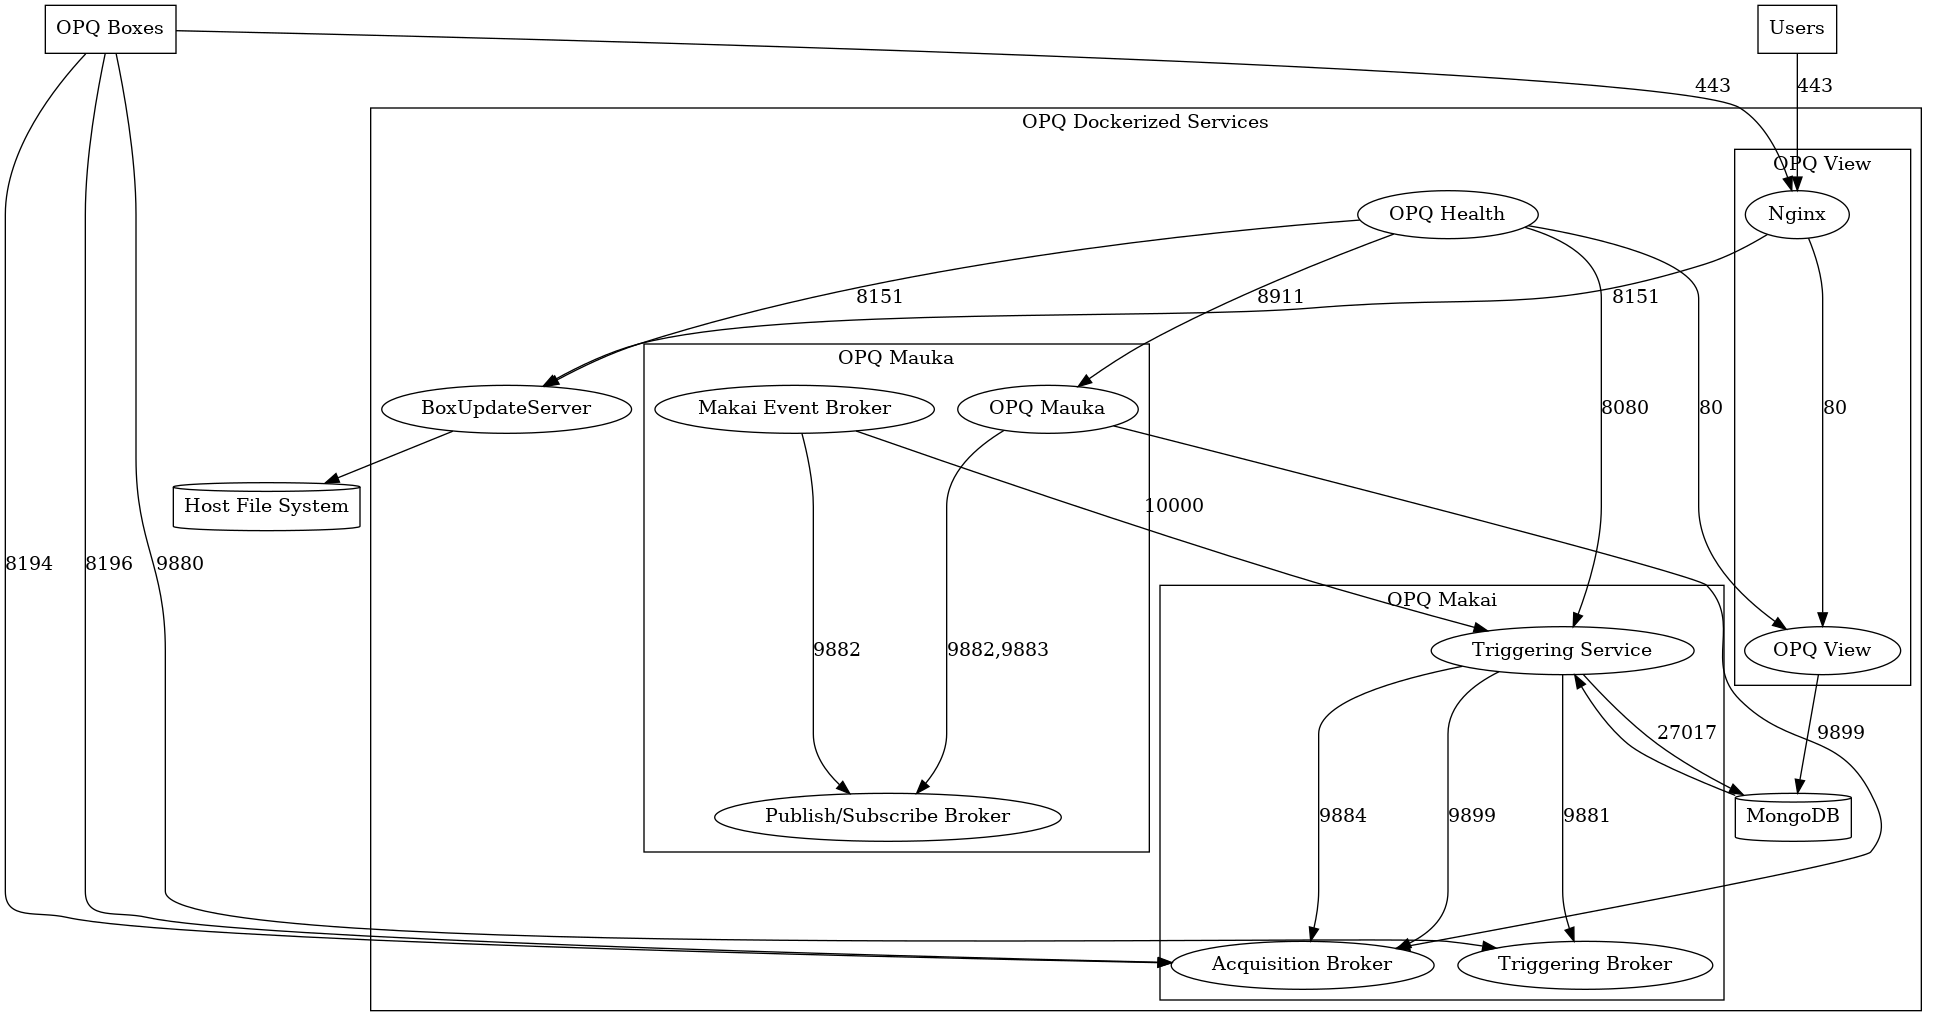
\includegraphics[width=1\linewidth]{figures/docker_deploy.png}
	\caption{OPQ Docker Architecture}\label{fig:docker_deploy}
\end{figure}

\section{Lokahi: A Laha-compliant Infrasound DSN}\label{sec:lokahi:-a-laha-compliant-infrasound-dsn}
Lokahi is a dynamic DSN that originally evolved as a distributed infrasound detection network. Infrasound is characterized as sound waves that are less than 20 Hz. Infrasound generally can not be deciphered by the human ear, but it can be detected using microphone and barometric pressure sensors. Any large movements of the atmosphere can produce infrasound. The Lokahi network was designed to supplement the International Monitoring System (IMS) for the capture  of undeclared and declared nuclear explosions. Lokahi has been successfully used to capture signals from volcanoes, hurricanes, aircraft, meteors, and other large atmospheric events.

Sensors in Lokahi are any mobile device that can run iOS or Android. We have sensors distributed world wide. The software stack for Lokahi consists of a distributed actor system for data acquisition, MongoDB for metadata persistence, Apache Kafka for data queues and interprocess communication, Python and related scientific libraries for analysis, and a distributed key-value store for long term storage or sensor data.

Recent development and improvements to the data API have allowed Lokahi to begin accepting data from any of the available onboard sensors on iOS and Android devices. Even though the main focus is still infrasound, having access to all of the available sensors provides the ability to sense other sensor fields and to perform interesting data fusion techniques.

A diagram of the Lokahi framework is provided in Figure~\ref{fig:lokahi}.

\begin{figure}
	\centering
	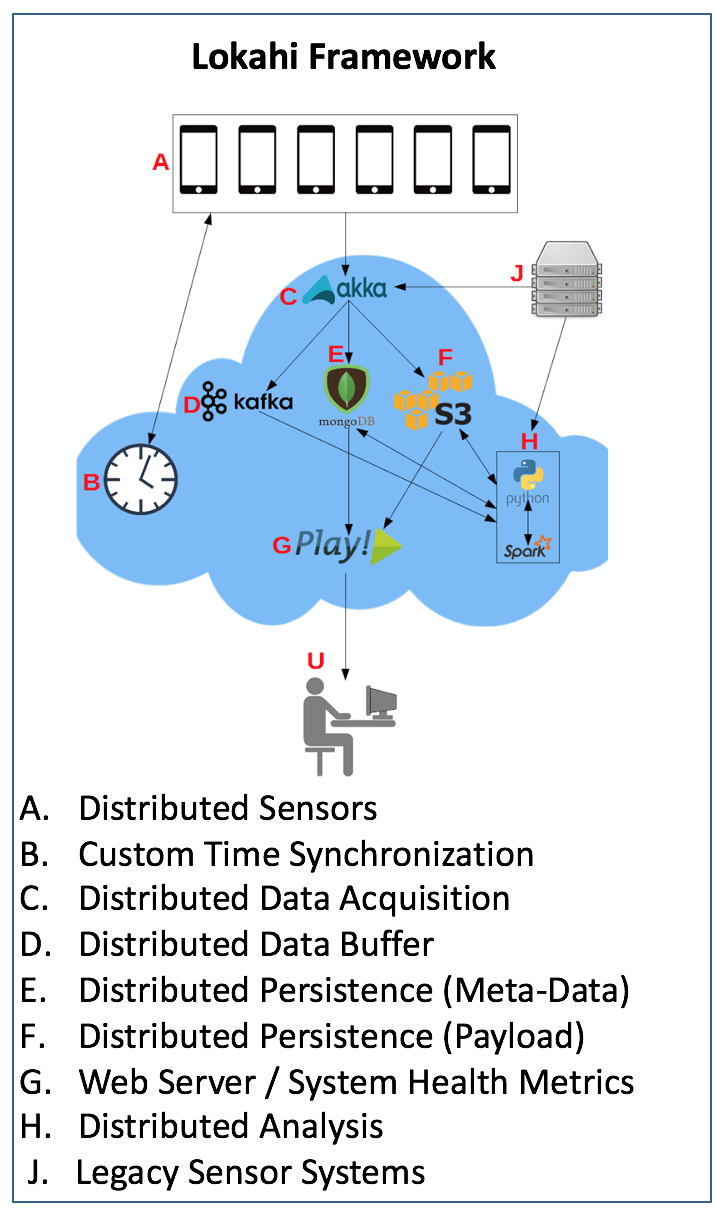
\includegraphics[]{figures/lokahi.png}
	\caption{Lokahi Design}\label{fig:lokahi}
\end{figure}

Lokahi is made up of several distributed services, each of which will be discussed in the following sections.

\subsection{Lokahi Data Acquisition Service}\label{subsec:lokahi-data-acquisition-service}
The data acquisition service is responsible for acquiring, authenticating, storing, and moving real-time sensor data from Lokahi sensors.

The data acquisition service is written in Rust~\cite{rust:2019} and makes use of Actix Actors~\cite{actix:2019} for scalability and distributed communication. Originally, the data acquisition server was written in Java using Akka Actors~\cite{akka:2019}. I recently moved the acquisition server to Rust so that it can be run on embedded hardware such as Raspberry Pis in resource restricted environments or on the edge of networks. Rust also provides performances improvements in terms of CPU utilization and memory utilization.

Type safe data is passed between actors where each actor fulfills a single purpose. When an actor successfully completes a unit of work, it responds with an empty success message to the calling actor. If an actor fails to complete a unit of work, it responds with a type safe error message to the calling actor. Errors messages are passed up the chain until they get to the original caller.

All actors in this service are optional and configurable. For instance, this service can be brought up with the sole purpose of writing the data to a file system and nothing else, or acting  solely as a data relay, or only storing data to AWS S3, or it can do it all.

Further, multiple Actors can be ran concurrently with different configurations. For instance, it is possible to define multiple Kafka~\cite{kreps2011kafka} actors, each with their own encryption and endpoint configurations, or you could write data to multiple file systems by configuring multiple file system Actors, etc.

It is also possible to configure each actor with whitelists and blacklists where items can be added by sensor Id or sensor owner. In this way, the configuration for each actor can be fine tuned to only allow certain sensors or sets of sensors or disallow sets of sensors. This is utilized when we require that only a subset of data received be forwarded to a particular actor. For instance, when we share real time data with our collaborators, they are only interested in a certain subset of data that we are receiving. Therefore, we create a whitelist with their information so that they only receive the data they are interested in. On the other hand, that data may be sensitive, so we black list it on other actors so that data is not forwarded to those actors.

Finally, configuration of all actors is performed declaratively in a type safe configuration file.

Figure~\ref{fig:LokahiAcquisition} provides an overview of the workflow and communication between Actors with the acquisition service.

\begin{figure}
	\centering
	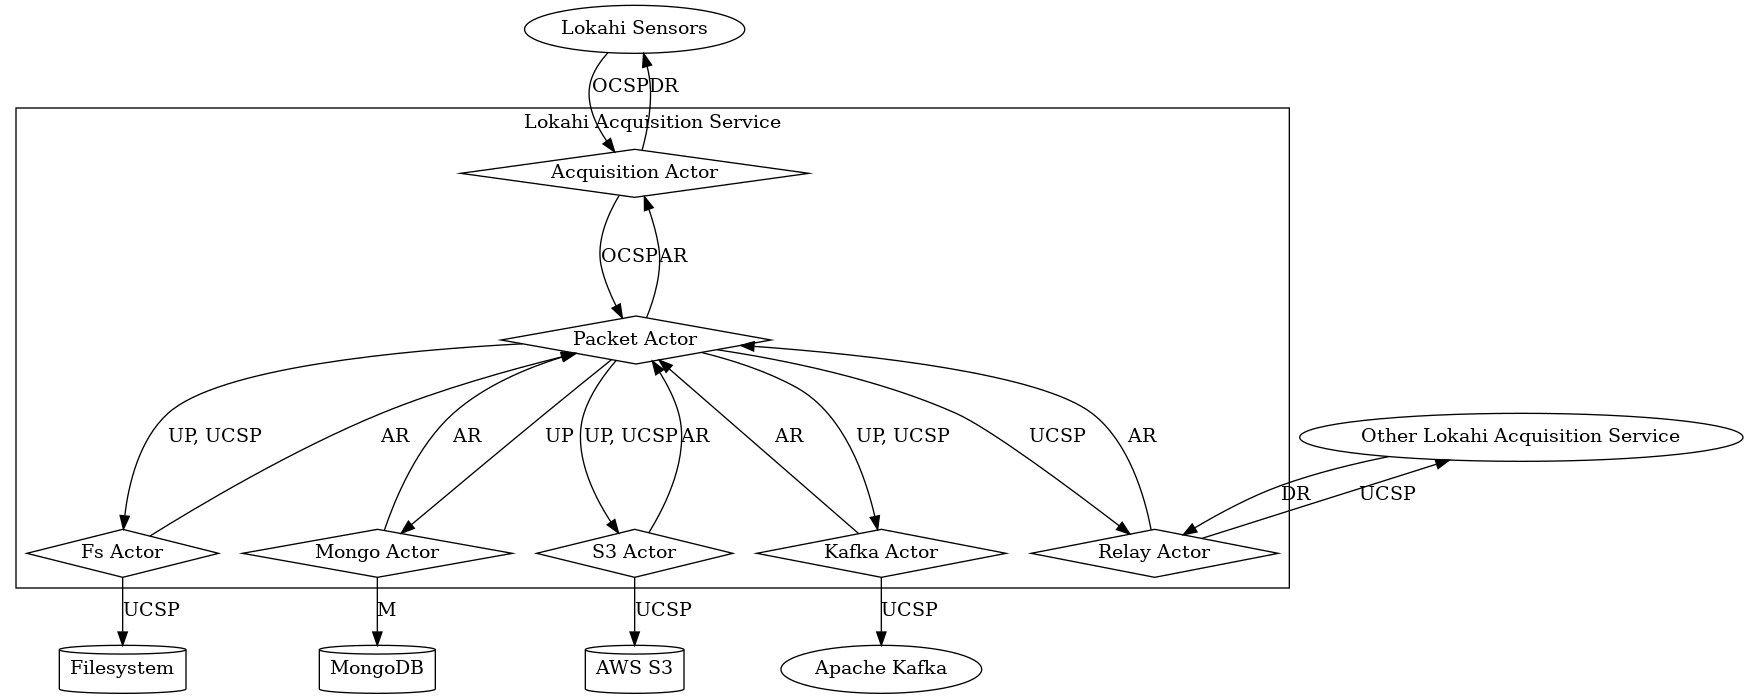
\includegraphics[width=\linewidth]{figures/lokahi_acquisition.png}
	\caption{Lokahi Acquisition Architecture where OCSP=``original compressed serialized packet", UP=``updated packet", UCSP=``updated compressed serialized packet", M=``metadata", AR=``actor response", DR=``device response".}
	\label{fig:LokahiAcquisition}
\end{figure}

\subsubsection{Acquisition Service Configuration}

Configuration for this service is stored in a .toml file. This file is parsed from the environment on service startup and deserialized into a typesafe Rust struct. The configuration is completely declarative and all actor configurations are optional. Also, it is possible to add new actors to this system by simply declaring a new actor in the configuration and restarting the service. This approach scales much more nicely than our previous approach which required editing the source code directly to modify or add actors.

An example configuration file with one of each actor type is provided in the appendix in Section~\ref{lokahi_acquisition_config}.

\subsubsection{Acquisition Actor}
Lokahi sensors establish an encrypted WebSocket connection to the the acquisition server in which they send data over. Encryption is provided over standard HTTPS using ``Let's Encrypt" as a certificate provider. Once the connection is established, the connection remains open for as long as the sensor is continuously sending data. Each connection causes the creation of a new Actix Actor within the acquisition service. Instead of creating a thread for each connection, actors share their resources over a configurable thread pool and lightweight green threads are used to provide concurrency. Since most of the work of the acquisition service is I/O bound, the system employs green threads.

This actor is also responsible for checking the response messages from all actors in the acquisition pipeline. If all responses are ``Ok", then this actor responds to the sensor with a checksum and an ``Ok" response. If any of the actor responses are an error, then this actor responds to the sensor with an error message and the sensor will store the data onboard until it is able to send at a later time.

\subsubsection{Packet Actor}
The acquisition service ``Packet Actor" handles each packet from a sensor individually. When a packet arrives, the packet is first decompressed using a custom LZ4 compression protocol where the first four bytes of the compressed payload contain the size of the original uncompressed data.

Once the packet is decompressed, it is then deserialized using Protocol Buffers into a struct that Rust is able to work with. The data packet protocol is provided in full in the appendix in Section~\ref{lokahi-data-packet-protocol}.

Each packet contains a Json Web Token (JWT) which is a cryptographically signed token generated by Lokahi Web. This token provides user authentication and authorization. The acquisition service extracts the token and either accepts or rejects the packet depending on if authentication is successful or not.

The acquisition service ``Packet Actor" performs several small updates to the packet when it arrives. First, it adds a server receive timestamp which marks the time that the packet was received at the server. This, along with the packet sensor time stamps allows us to keep a running record of latency values from sensors to acquisition service. Next, the authentication token and Firebase token are redacted since their values are only used within the acquisition service. This prevents others from accessing this data and masquerading as someone else. Finally, the packet is marked as either ``real-time" or ``backfilled" depending using a heuristic that compares the packet timestamps to the server timestamps. Real-time data is data that is recorded and immediately transferred over the network whereas backfilled data is recorded and sent over the network at a later time. Finally, the packet is updated with a data key which is the key that will eventually be used to store the data packet in AWS S3, a distributed key-value store.

\subsubsection{Mongo Actor}
Once the packet has been updated by the ``Packet Actor", all meta-data is extracted and stored in MongoDB by a ``Mongo Actor". Everything from the original packet is stored except for the data payloads themselves. However, the descriptive statistics of the payloads are stored so that the database contains some metadata about what the payload contains.

Multiple collections are updated by the Mongo Actor when a packet is received.

The ``RedvoxPacketApi900" collection stores metadata for all data packets received from sensors. The schema for this collection is described in Table~\ref{table:RedvoxPacketApi900}. This document also includes two embedded documents EvenlySampledChannel (Section~\ref{table:EvenlySampledChannel}) and UnevenlySampledChannel (Section~\ref{table:UnevenlySampledChannel}). The EvenlySampledChannel document contains metadata for evenly sampled channels such as the microphone. The UnevenlySampledChannel document contains metadata for unevenly sampled channels such as barometer, location, gyroscope, accelerometer, etc.

\begin{table}
	\centering
	\caption{RedvoxPacketApi900}
	\begin{tabularx}{\textwidth}{llX}
		\toprule
		\textbf{Field} & \textbf{Value} & \textbf{Description} \\
		\midrule
		\_id & bson.ObjectId & The object Id associated with the document. \\
		className & str & The class name used for Java serialization and deserialization. \\
		api & int32 & The API version of this data (should be 900). \\
		redvoxId & str & The Id of the sensor. \\
		redvoxUuid & str & The uuid of the sensor. \\
		authenticatedEmail & str & The user account associated with this device. \\
		authenticationToken & str & The JWT that was used for authenticating this packet. \\
		firebaseToken & str & The firebase token associated with this device. \\
		isBackfilled & bool & True if this packet was backfilled, False otherwise. \\
		isPrivate & bool & True if this packet is marked as private, False otherwise. \\
		isScrambled & bool & True if this packet has voice data scrambled, False otherwise. \\
		deviceMake & str & The make of the sensor. \\
		deviceModel & str & The model of the sensor. \\
		deviceOs & str & The OS of the sensor (either iOS or Android). \\
		deviceOsVersion & str & The OS version. \\
		appVersion & str & The sensor app version. \\
		batteryLevelPercent & f32 & The sensor's battery level. \\
		deviceTemperatureC & f32 & The sensor's temperature in C. \\
		acquisitionServer & str & The server that this data was sent to. \\
		timeSynchronizationServer & str & The server this sensor used for synch. \\
		authenticationServer & str & The server this sensor used to authenticated with. \\
		appFileStartUsUtc & i64 & The timestamp of the start of this packet. \\
		appFileStartMachine & i64 & The machine timestamp of the start of this packet. \\
		serverTimestampUsUtc & i64 & The time that this packet was received at the server. \\
		evenlySampledChannels & [EvenChannel] & Evenly sampled channels metadata. \\
		unevenlySampledChannels& [UnevenChannel] & Unevenly sampled channels metadata. \\
		metadata & [str] & A list of metadata added to this packet. \\
		dataKey & str & The location of the original data file stored in AWS S3. \\
		\bottomrule
	\end{tabularx}
	\label{table:RedvoxPacketApi900}
\end{table}

\begin{table}[H]
	\centering
	\caption{RedvoxPacketApi900.EvenlySampledChannel}
	\begin{tabularx}{\textwidth}{llX}
		\toprule
		\textbf{Field} & \textbf{Value} & \textbf{Description} \\
		\midrule
		channelTypes & [str] & A list of sub-channels included in this channel. \\
		sensorName & str & The name of sensor. \\
		sampleRateHz & f64 & The sample rate of this sensor. \\
		firstSampleTimestampUs & i64 & Timestamp of the first sample. \\
		payloadCase & str & An enum string for the data type stored in the payload. \\
		payloadCount & i32 & The number of items in the payload in the original data. \\
		valueMeans & [f64] & List of mean values of the payload for each sub-channel. \\
		valueStds & [f64] & List of the stddev of the values of the payload for each sub-channel. \\
		valueMedians & [f64] & List of medians of the values of the payload for each sub-channel. \\
		metadata & [str] & List of metadata added to this channel. \\
		\bottomrule
	\end{tabularx}
	\label{table:EvenlySampledChannel}
\end{table}

\begin{table}[H]
	\centering
	\caption{RedvoxPacketApi900.UnevenlySampledChannel}
	\begin{tabularx}{\textwidth}{llX}
		\toprule
		\textbf{Field} & \textbf{Value} & \textbf{Description} \\
		\midrule
		channelTypes & [str] & A list of sub-channels included in this channel. \\
		sensorName & str & The name of sensor. \\
		timestampsCount & i32 & The number of timestamps for this channel in the original data. \\
		payloadCase & str & An enum string for the data type stored in the payload. \\
		payloadCount & i32 & The number of items in the payload in the original data. \\
		valueMeans & [f64] & List of mean values of the payload for each sub-channel. \\
		valueStds & [f64] & List of the stddev of the values of the payload for each sub-channel. \\
		valueMedians & [f64] & List of medians of the values of the payload for each sub-channel. \\
		sampleIntervalMean & f64 & The mean sample interval of each sample. \\
		sampleIntervalStd & f64 & The mean sample stddev of each sample. \\
		sampleIntervalMedian & f64 & The median sample interval of each sample. \\
		metadata & [str] & List of metadata added to this channel. \\
		\bottomrule
	\end{tabularx}
	\label{table:UnevenlySampledChannel}
\end{table}

The Mongo Actor also updates other documents which are used by Lokahi View for display, device, and user management. The schemas for these collections are described next.

The ``RedvoxDeviceApi900" collection contains metadata relating to each sensor that Lokahi receives from. This collection is described in Table~\ref{table:RedvoxDeviceApi900}. This collection also contains two embedded documents ``PrivacyPolicy" (Section~\ref{table:PrivacyPolicy}) and ``AuthenticatedEmailEntry" (Section~\ref{table:AuthenticatedEmailEntry}).

\begin{table}[H]
	\centering
	\caption{RedvoxDeviceApi900}
	\begin{tabularx}{\textwidth}{llX}
		\toprule
		\textbf{Field} & \textbf{Value} & \textbf{Description} \\
		\midrule
		\_id & bson.ObjectId & The object Id of this document. \\
		className & str & Used for Java ORM interop. \\
		redvoxId & str & The Id associated with this device. \\
		uuid & str & The uuid associated with this device. \\
		lastUpdatedTimestamp & i64 & The timestamp of the last time this device received data. \\
		lastPacket & DBRef & A reference to the last received packet. \\
		lastLocationPoint & mongo.Point & The last location this device was received from. \\
		currentPolicyType & str & The devices policy type (public/private). \\
		privacyPolicies & [PrivacyPolicy] & A list of privacy policies this device has used. \\
		currentAuthenticatedEmail & str & This devices current user. \\
		authenticatedEmailEntries & [AuthenticatedEmailEntry] & A list of all users who have used this device. \\
		valid & bool & A field that marks this device as valid or invalid. \\
		receivers & [str] & A list of users who can access data from this device. \\
		\bottomrule
	\end{tabularx}
	\label{table:RedvoxDeviceApi900}
\end{table}

\begin{table}[H]
	\centering
	\caption{PrivacyPolicy}
	\begin{tabularx}{\textwidth}{llX}
		\toprule
		\textbf{Field} & \textbf{Value} & \textbf{Description} \\
		\midrule
		policyType & str & A string representing the policy type (public/private). \\
		startTimestampMillisecondsSinceEpochUtc & i64 & Start time of this policy. \\
		\bottomrule
	\end{tabularx}
	\label{table:PrivacyPolicy}
\end{table}

\begin{table}[H]
	\centering
	\caption{AuthenticatedEmailEntry}
	\begin{tabularx}{\textwidth}{XlX}
		\toprule
		\textbf{Field} & \textbf{Value} & \textbf{Description} \\
		\midrule
		authenticatedEmail & str & The email associated with this account at this time. \\
		startTimestampMillisecondsSinceEpochUtc & i64 & Start time of this email entry. \\
		\bottomrule
	\end{tabularx}
	\label{table:AuthenticatedEmailEntry}
\end{table}

The ``HistoricalDevice" collection is used to store metadata about the last data that was received for each sensor. This is used in Lokahi View for displaying the location of every sensor ever received. The HistoricalDevice collection is described in Table~\ref{table:HistoricalDevice}.

\begin{table}[H]
	\centering
	\caption{HistoricalDevice}
	\begin{tabularx}{\textwidth}{llX}
		\toprule
		\textbf{Field} & \textbf{Value} & \textbf{Description} \\
		\midrule
		deviceId & i64 & The sensor Id. \\
		uuid & i64 & The sensor uuid. \\
		lastActive & Date & The last time this device was active. \\
		lastLocation & mongodb.Point & The last location this device was received from. \\
		os & str & The OS of this device as of its last sent packet. \\
		\bottomrule
	\end{tabularx}
	\label{table:HistoricalDevice}
\end{table}

The ``DailyDataUsage" collection is a collection that stores metadata relating to how much data is used daily per user of the Lokahi service. The ``DailyDataUsage" document schema is provided in Table~\ref{table:DailyDataUsage}.

\begin{table}[H]
	\centering
	\caption{DailyDataUsage}
	\begin{tabularx}{\textwidth}{llX}
		\toprule
		\textbf{Field} & \textbf{Type} & \textbf{Description} \\
		\midrule
		\_id & bson.ObjectId & The object Id of this document. \\
		user & str & The user account associated with this document. \\
		year & int32 & The year of this document. \\
		month & int32 & The month of this document. \\
		day & int32 & The day of this document. \\
		bytesContributed & int64 & The number of bytes contributed by this user. \\
		bytesConsumed & int64 & The number of bytes consumed by this user. \\
		\bottomrule
	\end{tabularx}
	\label{table:DailyDataUsage}
\end{table}

\subsubsection{S3 Actor}
After the metadata has been stored, the updated packet is serialized back into bytes and then compressed using the same custom LZ4  compression protocol. This data is then sent to AWS S3 by the ``S3 Actor" for permanent storage for later data retrieval. S3 is a cloud service offered by Amazon which acts as a distributed key-value store with essentially unlimited space.

Data is stored to S3 using using the following directory layout:

api900/[YYYY]/[MM]/[DD]/[sensor\_id]\_[packet\_timestamp\_ms].rdvxz.

\subsubsection{Fs Actor}
The data can optionally be stored to any accessible file system using the ``Fs Actor". This is useful in cases when your acquisition server may only have local network access, such as restricted sites with an acquisition server running on a Raspberry Pi on a LAN\@.

\subsubsection{Kafka Actor}
The compressed data is next produced to several Apache Kafka~\cite{kreps2011kafka} endpoints using the ``Kafka Actor".

Apache Kafka provides a distributed messaging queue that can use publish/subscribe semantics. Lokahi uses Kafka for inter-process distributed communication and for providing a real-time data endpoint for our collaborators. Lokahi manages an internal Kafka queue that acts as a ring buffer for storing an hours worth of real-time data for each device. This real-time ring buffer is used for generating real time plots of data without needing to access the database or pull the data from AWS S3.

Lokahi also provides secure real-time Kafka endpoints to our collaborators which include national labs, defense contractors, and private contracts. The acquisition service filters collaborator packets based off of the JWT and encrypts the compressed serialized packet with the collaborator's GPG public key. Our collaborators then use an Apache NiFi service for collecting and decrypting the data from the Kafka endpoint for their own internal use.

Each device is provided its own partition within Kafka to publish data to. Since each Kafka partition creates a file on the file system, the number of Kafka partitions and the partitions themselves must be managed intelligently. Partitions are assigned by the acquisition service. The acquisition service looks up the next available partition in the database. Partitions become available if a sensor stops using a partition for longer than an hour. Our current design provides up to 500 concurrent partitions at once.

\subsubsection{Relay Actor}
The acquisition service can act as a relay to other acquisition services that speak the same protocol. If this actor is enabled, any packets it receives are relayed to the configured acquisition server. This is useful for load balancing and for timing accuracy. In load balancing, this server can be configured to filter subsets of devices to other acquisition servers by configuring a relay actor for each server that data is being forwarded to. For timing accuracy, this service can be deployed on a Raspberry Pi at the edge of a network near the sensors, reducing the latency between sensor and server. Then, when a packet arrives at the server, it is updated with a low latency server timestamp which improves timing accuracy. The low powered Raspberry Pi can then relay the packet to the cloud where it will be handled, but already have the improved timing accuracy built into the packet.

\subsection{Lokahi Time Synchronization}\label{subsec:lokahi-time-synchronization}
Much of Lokahi's sensor analysis requires that sensors be synchronized in time. In order to calculate direction and distance to a signal source, sensors should have clocks that are synchronized within milliseconds of each other. We initially tried to use NTP, but it did not provide the timing accuracy we desired, and thus, implemented a custom time synchronization protocol.

The protocol used in Lokahi is an implementation described by Tian et al in their Tri-Message Exchange paper\cite{tian2009tri}. This algorithm was developed specifically for providing accurate time synchronization in high latency networks.

This service is written in Rust and utilizes encrypted x for communication with sensors. While a sensor is recording data, a separate thread on that sensor continuously performs message exchanges with this service. The best exchange out of a group of exchanges (the one with the lowest latency) is then used to correct timing for packets.

A description of the algorithm is provided below. This algorithm expects that the client will build up a successive message exchange consisting of the elements B0, B1, B2, B3, A1, A2, A3, but only up two a maximum of two timestamps are ever exchanged at one time. These coefficients are then stored in each data packet so that the server can use them to correct for timing.

\begin{enumerate}
	\item Client connects to redvox-synch-server over WebSocket connection
	\item Client records and stores B0 immediately before sending message
	\item Client sends binary message to server where the payload is a single byte 0x00
	\item Server responds asynchronously, goto 5
	\item onMessage fires for client
	\begin{enumerate}
		\item Client records Btmp
		\item Client decodes payload (see protocol below)
		\item If sequence number is 0, then
		\begin{enumerate}
			\item Client extracts and stores A1 from server receive timestamp
			\item Client stores B1 = Btmp
			\item Client records and stores B2 immediately before sending message
			\item Client sends binary message to server where payload is a single byte 0x01
			\item Server responds asynchronously, goto 5
		\end{enumerate}
		\item If sequence number is 1, then
		\begin{enumerate}
			\item Client extracts and stores A2 from server receive timestamp
			\item Client extracts and stores A3 from server send timestamp
			\item Client stores B3 = Btmp
			\item Client can close the connection or reuse the same connection to perform another message exchange starting from 2
		\end{enumerate}
	\end{enumerate}
\end{enumerate}

The protocol used for communicating message exchanges is a simple binary protocol designed to reduce bandwidth. The protocol is described in detail in Table~\ref{table:syncproto}.

\begin{table}[H]
	\centering
	\caption{Time Synchronization Binary Protocol}
	\begin{tabularx}{\textwidth}{llX}
		\toprule
		\textbf{Byte} & \textbf{Offset} & \textbf{Description} \\
		\midrule
		0 & 1 & Sequence Number (0 or 1) \\
		1 &  8 & Int timestamp A $\mu\sec$  \\
		9 & 8 & Int timestamp B $\mu\sec$ \\
		\bottomrule
	\end{tabularx}
	\label{table:syncproto}
\end{table}


\subsection{Lokahi Health}\label{subsec:lokahi-health}
System health is provided by three open source components Prometheus, Grafana, and node\_exporter. Prometheus is a time series database for metric collection and Grafana is a visualization solution for time series databases. ``node\_exporter" is installed on each system for collecting system statistics and sending them to a Prometheus endpoint. With these three systems, we are able to provide coverage for all performance metrics required by Lokahi.

\subsubsection{Up/Down Metrics}
node\_exporter, other than collecting system statistics, provides a simple metric for whether or not a system or service is up or down. This provides a base line of performance metrics. When a system goes down, an e-mail alert is sent to all interested parties. An example of our Up/Down interface is provided in Figure~\ref{fig:updown} which shows which services are currently working and which services require maintenance.

\begin{figure}
	\centering
	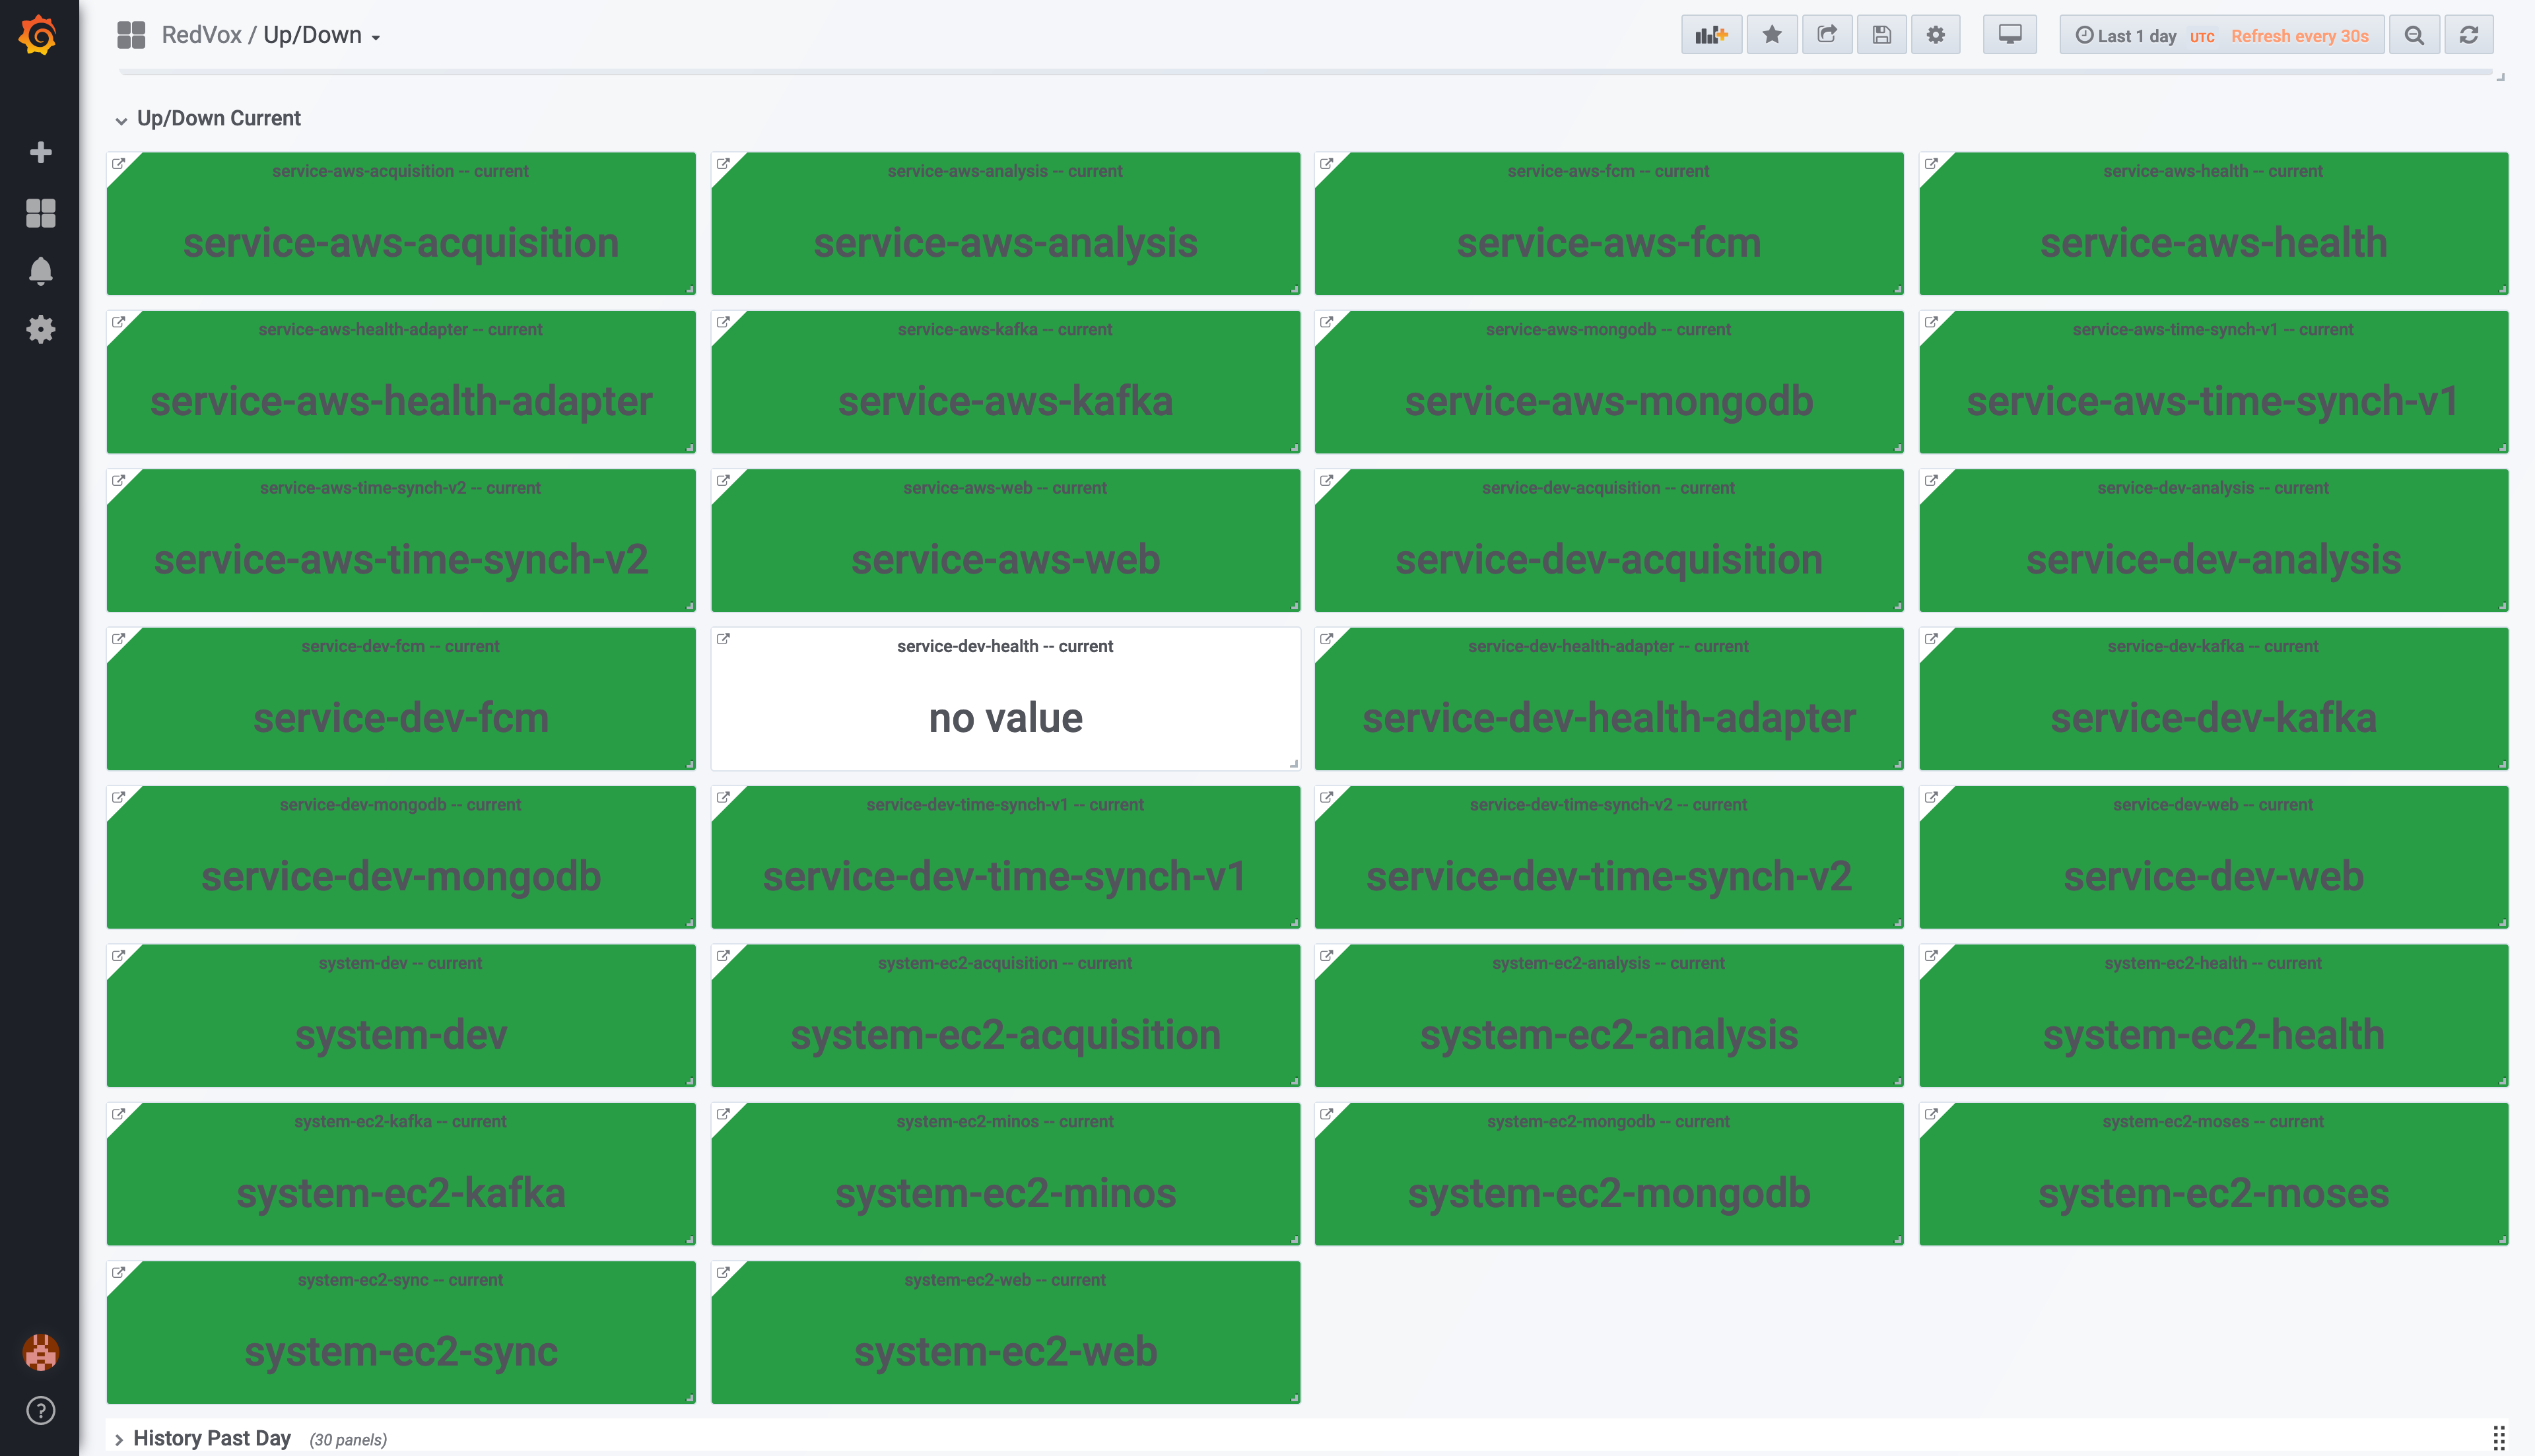
\includegraphics[width=\linewidth]{figures/updown.png}
	\caption{System and Service Status}
	\label{fig:updown}
\end{figure}

It is also possible to display a historic view up Up/Down metrics as shown in Figure~\ref{fig:updownhist}. When services are up, they display a value of ``1" and when services are down, the plot drops below ``1" indicating that the service was down for a certain amount of time.

\begin{figure}
	\centering
	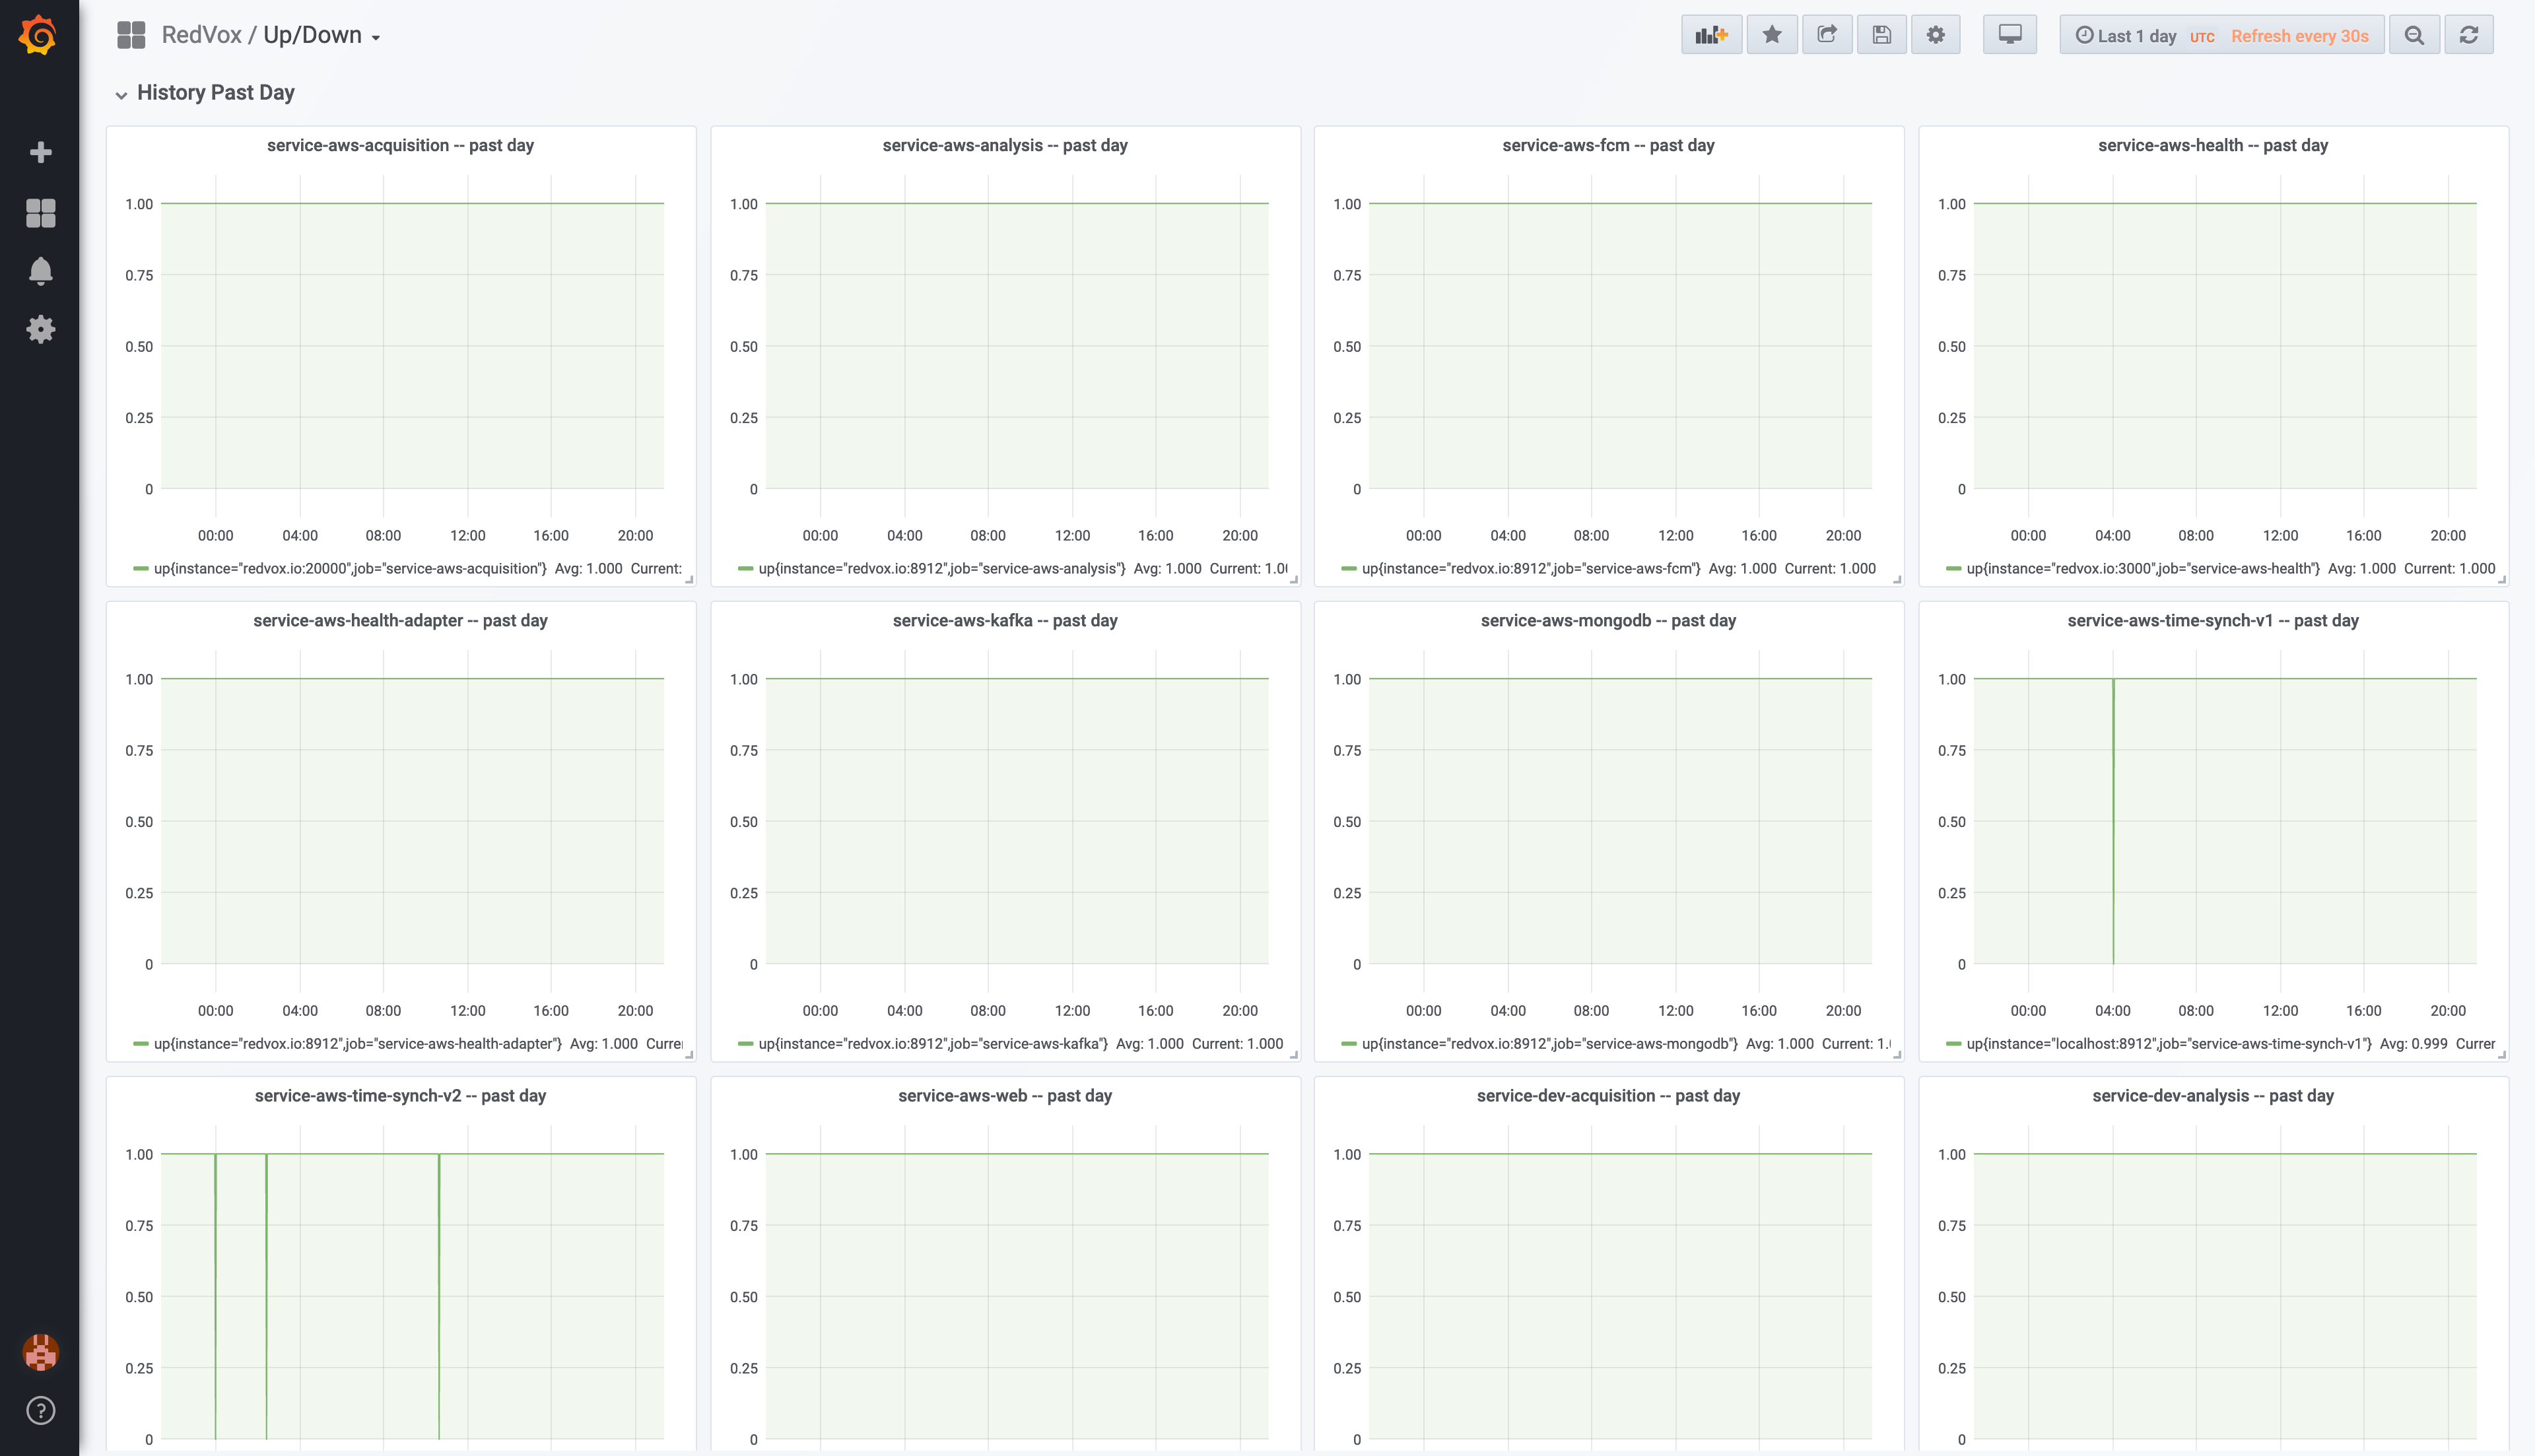
\includegraphics[width=\linewidth]{figures/updownhist.png}
	\caption{System and Service Status History Past Day}
	\label{fig:updownhist}
\end{figure}

\subsubsection{System Metrics}

``node\_exporter" provides Prometheus with a large selection of system metrics. We collect these metrics for each virtual server that we are running. We collect metrics on file system usage, memory usage, CPU usage, and network usage. An example of this from one of our services is displayed in Figure~\ref{fig:systemstats}.

\begin{figure}
	\centering
	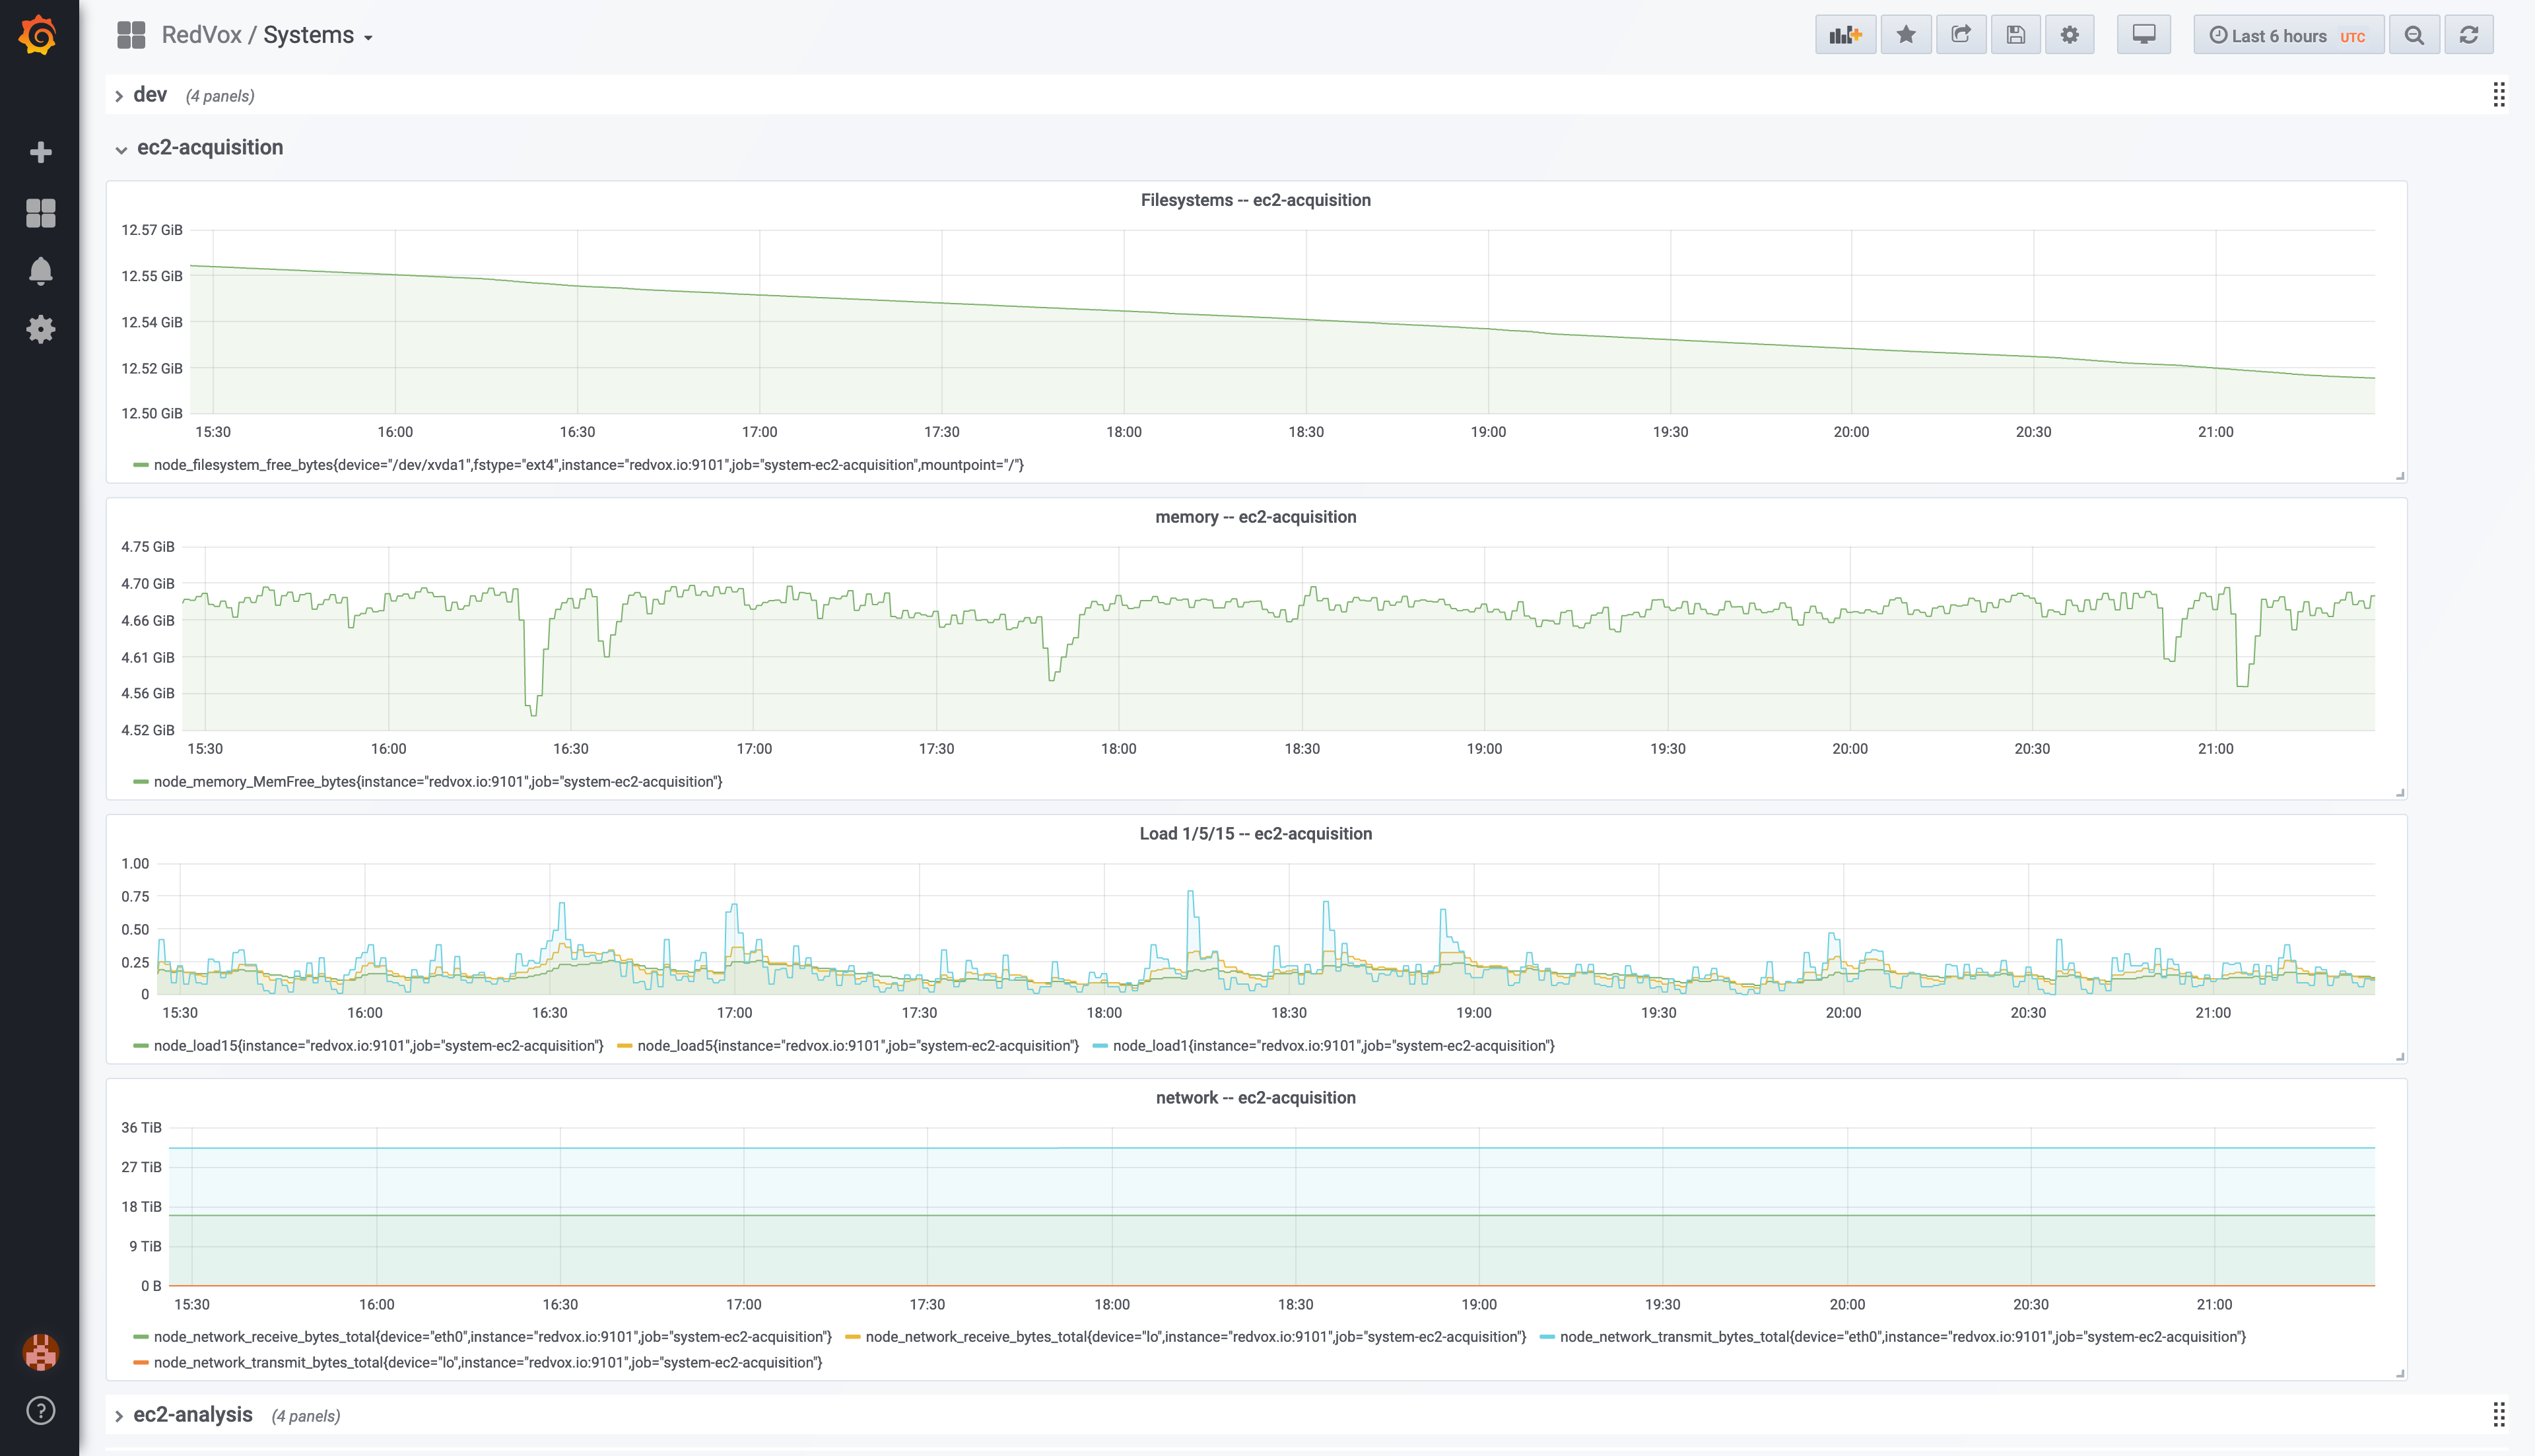
\includegraphics[width=\linewidth]{figures/systemstats.png}
	\caption{System Metrics}
	\label{fig:systemstats}
\end{figure}

\subsubsection{Sensor Metrics}

Lokahi also collects metrics from devices grouped by device and also grouped by device owner. We collect metrics on number of packets received and number of bytes received. We also collection metrics on sensor metadata such as device make/model, operating system, and app version. Due to the sensitive nature of this data, I will not provide a screenshot of these metrics. However, they are line graphs similar the system metrics.

\subsection{Lokahi Analysis}\label{subsec:lokahi-analysis}
Analysis of sensor data is provided by a custom Python framework. This framework utilizes an Apache Kafka client to subscribe to data request topics and real-time data topics.

When a request for analysis is received, the analysis framework will create a new process pool to run all of the analysis. Once the analysis is completed, the process pool is destroyed freeing up memory leaks caused by matplotlib. Requests for analysis include a time window, the devices that should be included for analysis, and the types of analysis that should be performed for those devices.

If the request is for real-time data, then the process will acquire the data from the Kafka real-time ring buffer data queue. If the request is for historic data, then the associated data will be looked up in the MongoDB database, and then the data payloads will be retrieved from AWS S3.

When the analysis is completed, metadata data about the analysis is stored to MongoDB, any figures generated by analysis are stored to AWS S3, and a response is sent back to Lokahi Web with the results of the analysis.

Lokahi Analysis is capable of creating the following products from sensor data:

\begin{itemize}
	\item Linear Microphone Waveform and Fast Fourier Transform (FFT)
	\item Log Microphone Waveform and FFT
	\item Multiresolution Microphone
	\item Barometer FFT
	\item Multiresolution Barometer
	\item Latency statistical line plot
	\item Location (latitude, longitude, altitude, speed) statistical line plot
	\item Magnetometer Waveform and FFT
	\item Gyroscope Waveform and FFT
	\item Accelerometer Waveform and FFT
	\item Light Waveform and FFT
\end{itemize}

In the above list, ``FFT" stands for Fast Fourier Transform which converts a signal from the time domain into the frequency domain for frequency analysis.

Figures are generating using Python's matplotlib library. Most of the sensor analysis was implemented by colleagues at the Infrasound Laboratory in Kailua-Kona. I merely provided the infrastructure that allows them to run their geophysical analysis.

The analysis framework is not only capable of producing new reports and products, but can also be used to update existing reports and products.

An overview of the analysis architecture is provided in Figure~\ref{fig:analysis_architecture}.

\begin{figure}
	\centering
	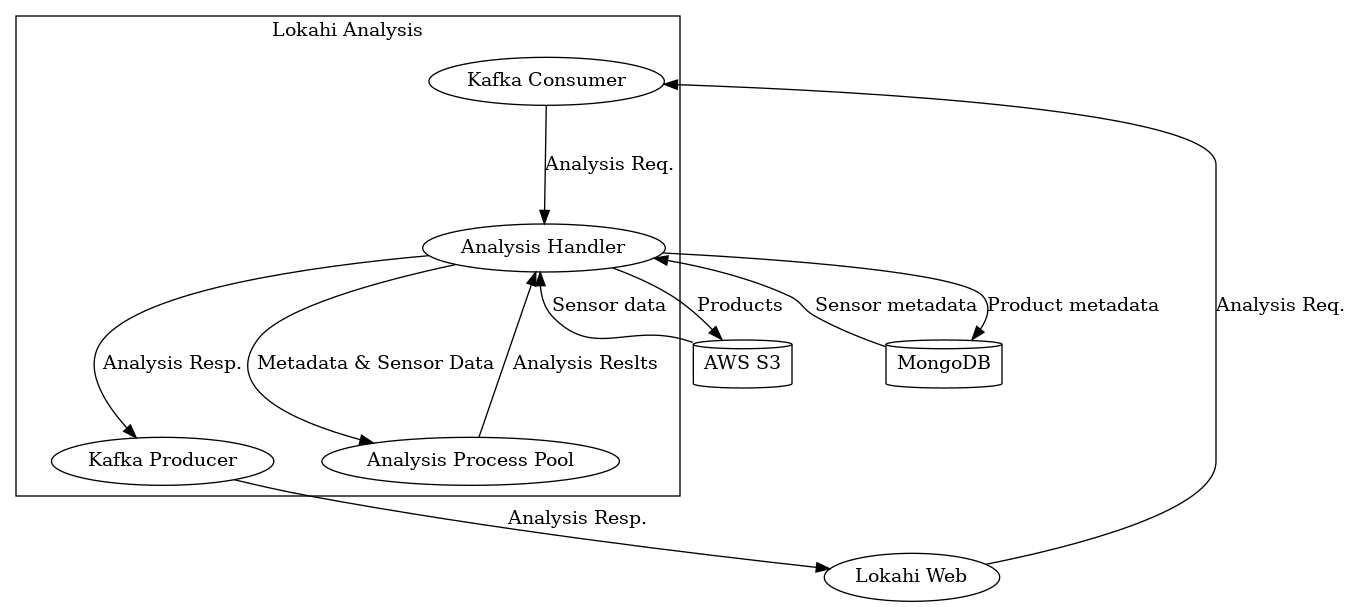
\includegraphics[width=\linewidth]{figures/analysis_architecture.png}
	\caption{Lokahi Analysis Architecture}
	\label{fig:analysis_architecture}
\end{figure}

\subsection{Lokahi Web}\label{subsec:lokahi-web}
Lokahi Web is a web interface that allows users to check the status of their sensors, download sensor data, and generate analysis reports. It also allows administrators to view sensor data usage, send alerts to sensors, and manage users. Lokahi Web is written in Java and powered by the Play Framework. Most functionality in Lokahi Web is provided from metadata stored in the MongoDB and by passing messages band and forth to the analysis service over a Kafka queue.

\subsubsection{Sensor Status}
The main page of Lokahi Web displays a map of currently active sensors (that the logged in user can access) and displays a list of those sensors sorted by distance from the users current location. This data is obtained by loading metadata from the database. An example if this interface is displayed in Figure~\ref{fig:lweb_main}.

\begin{figure}
	\centering
	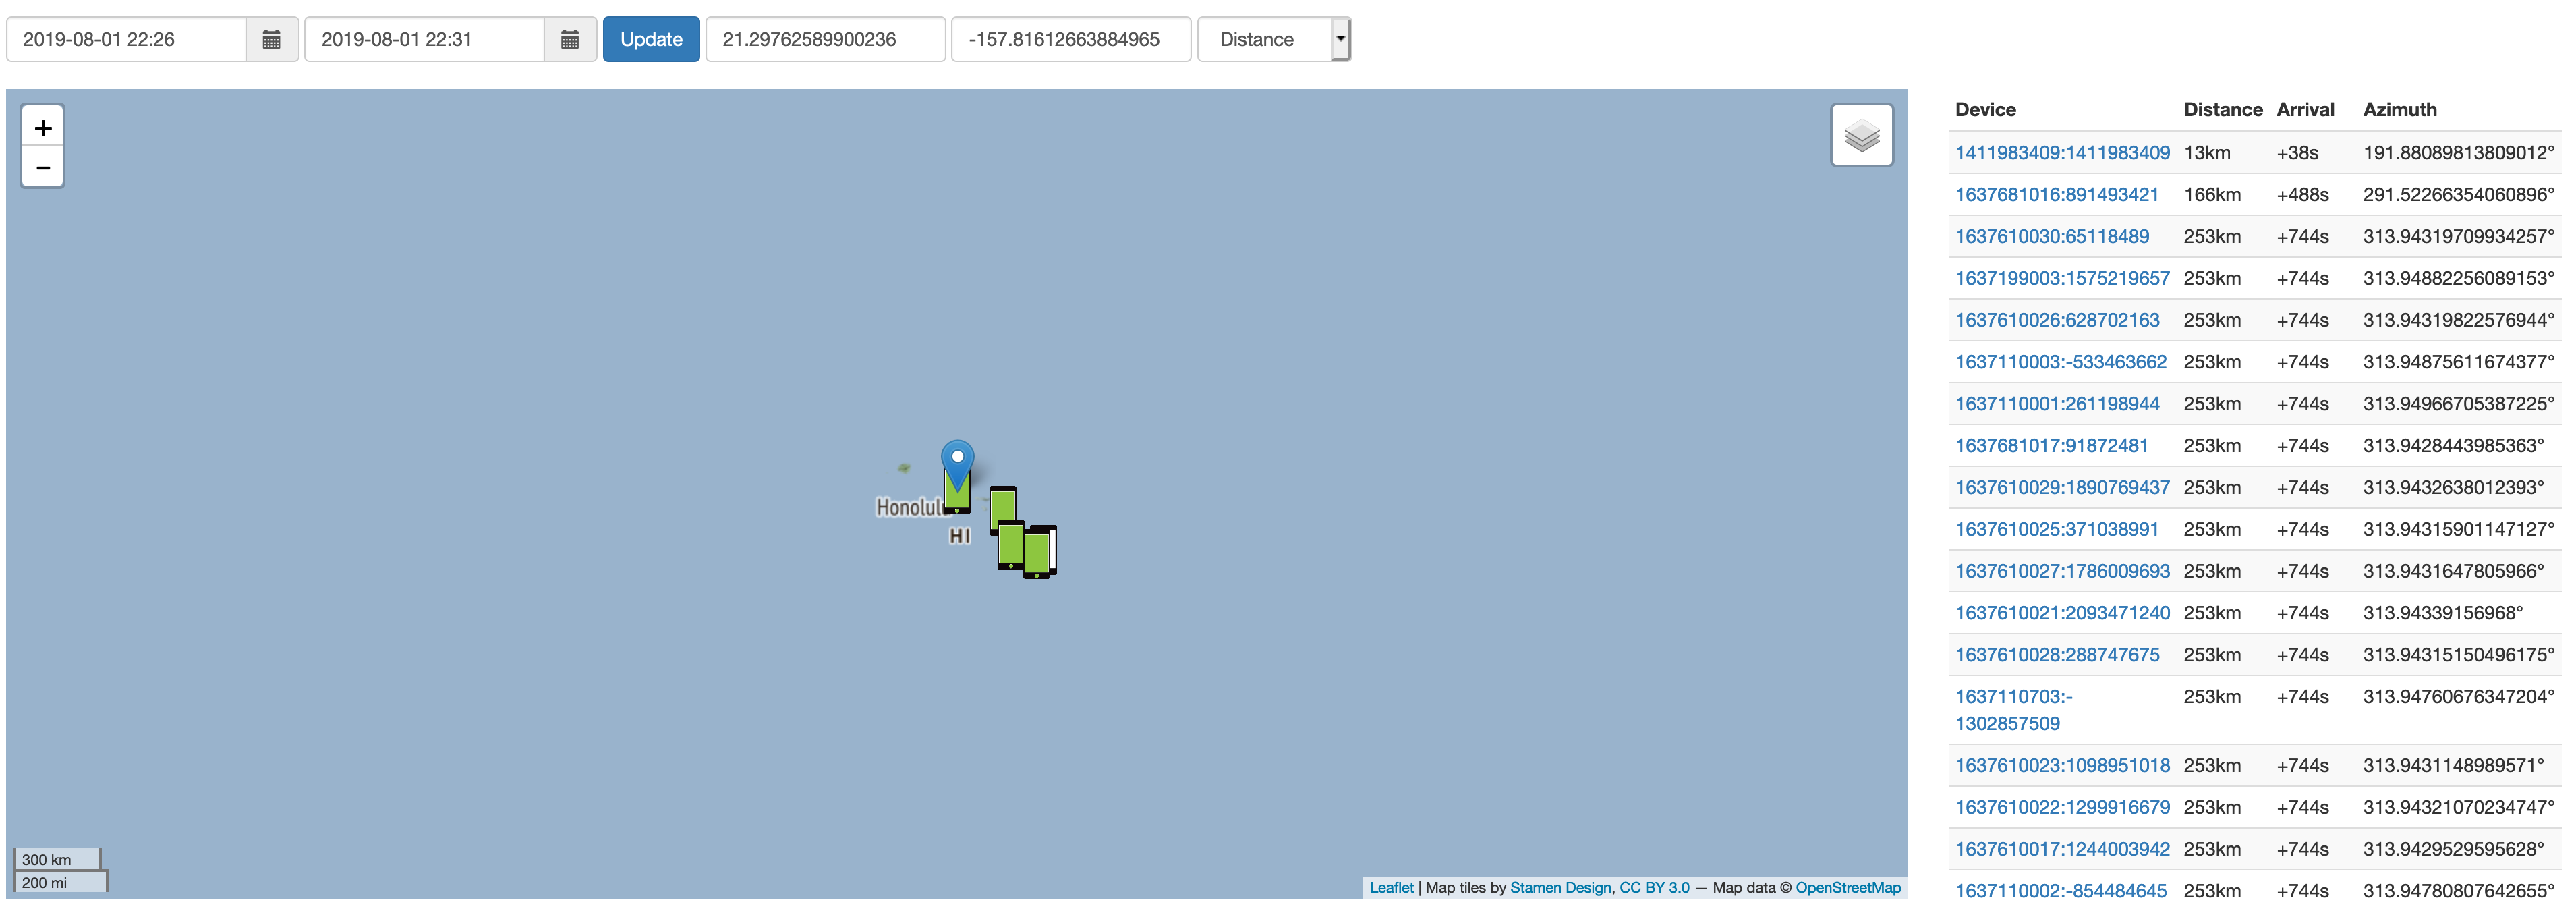
\includegraphics[width=\linewidth]{figures/lweb_main.png}
	\caption{Lokahi Web Main Page}
	\label{fig:lweb_main}
\end{figure}

The ``Active Devices" page lists all active devices that the logged in user can access as well as some metadata about those sensors. This data is loaded as metadata from the database. An example of this page is displayed in Figure~\ref{fig:lweb_status}.

\begin{figure}
	\centering
	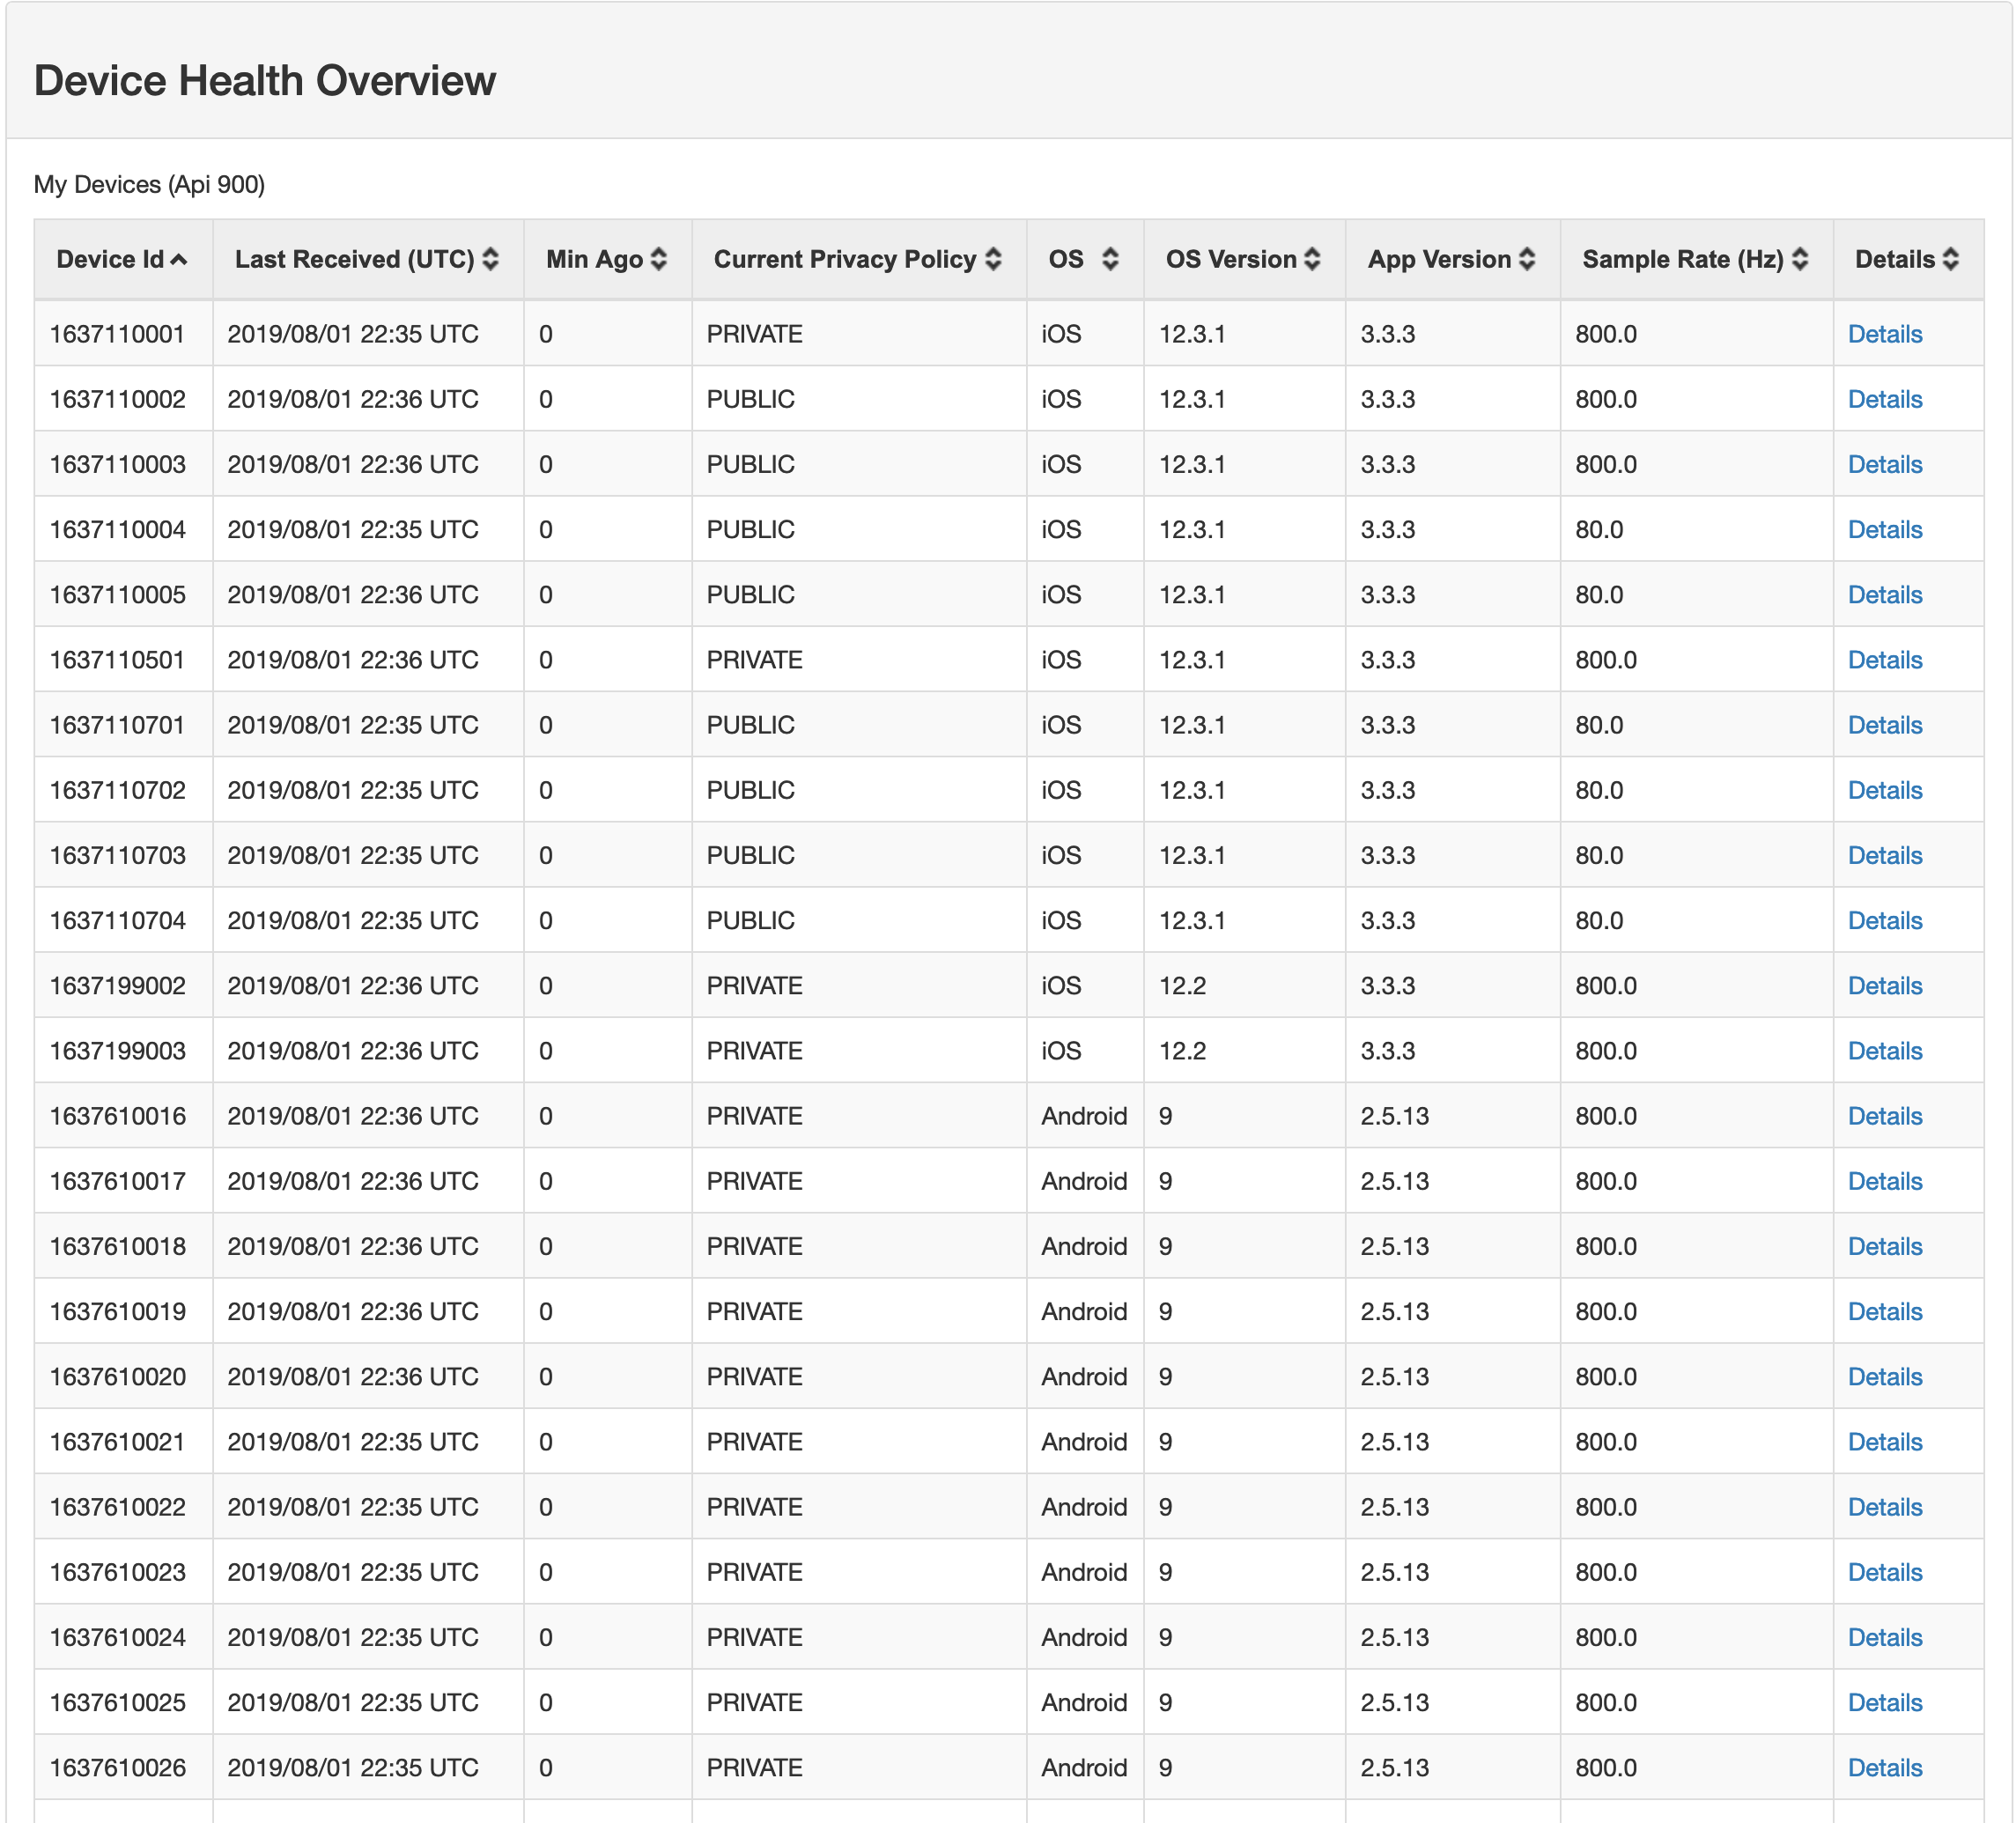
\includegraphics[width=\linewidth]{figures/lweb_status.png}
	\caption{Active Devices}
	\label{fig:lweb_status}
\end{figure}

It is possible to drill into the details of an individual device by clicking the ``Details" link on the ``Active Devices" page. The detailed device status includes a map of the location of the device, the device activity over the past hour and past day, metadata details, and real-time plots for microphone, barometer, location, and time synchronization This data is loaded as metadata from the database and also real-time sensor payload data is retrieved from the real-time Kafka ring buffer. An example of detailed device status is provided in Figure~\ref{fig:lweb_detail}.

\begin{figure}
	\centering
	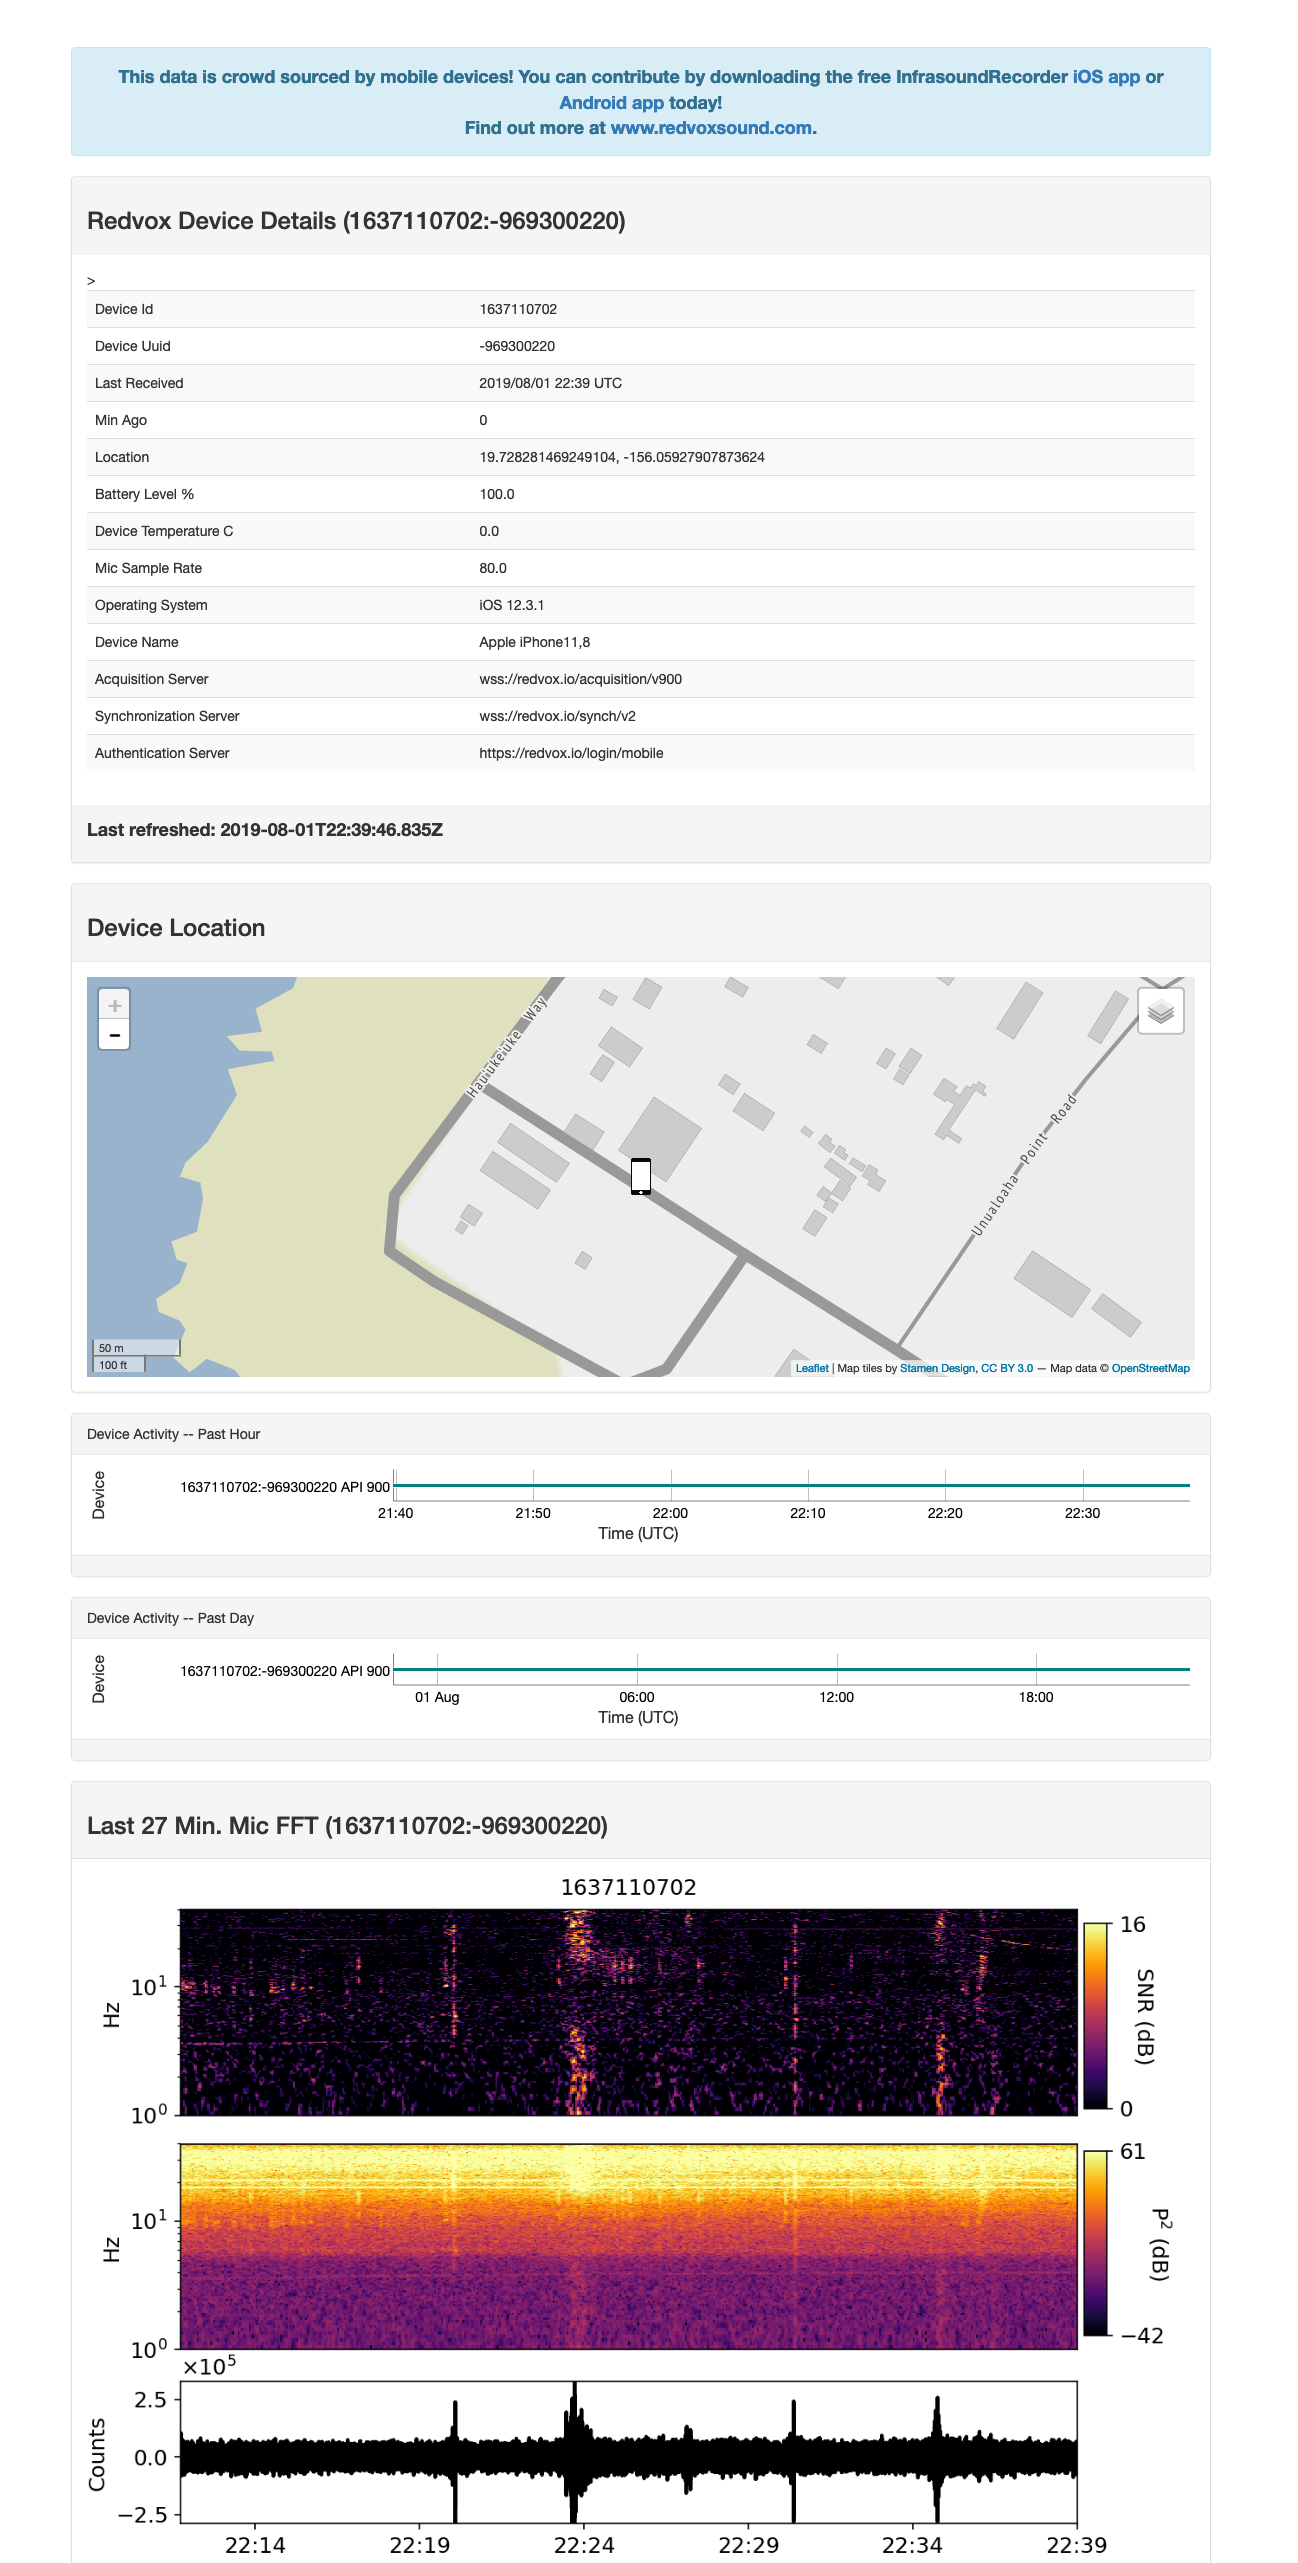
\includegraphics[width=0.7\linewidth]{figures/lweb_detail.png}
	\caption{Detailed Device Status}
	\label{fig:lweb_detail}
\end{figure}

Users are able to create groups of devices based on geo-location by defining a bounding box. Then all sensors that are within that bounding box will appear in that user created group. This allows users to view the status of multiple devices at one time for a specific geographic location. This data is stored as metadata in the database. An example of the group creation interface is displayed in Figure~\ref{fig:lweb_groupcreate}.

\begin{figure}
	\centering
	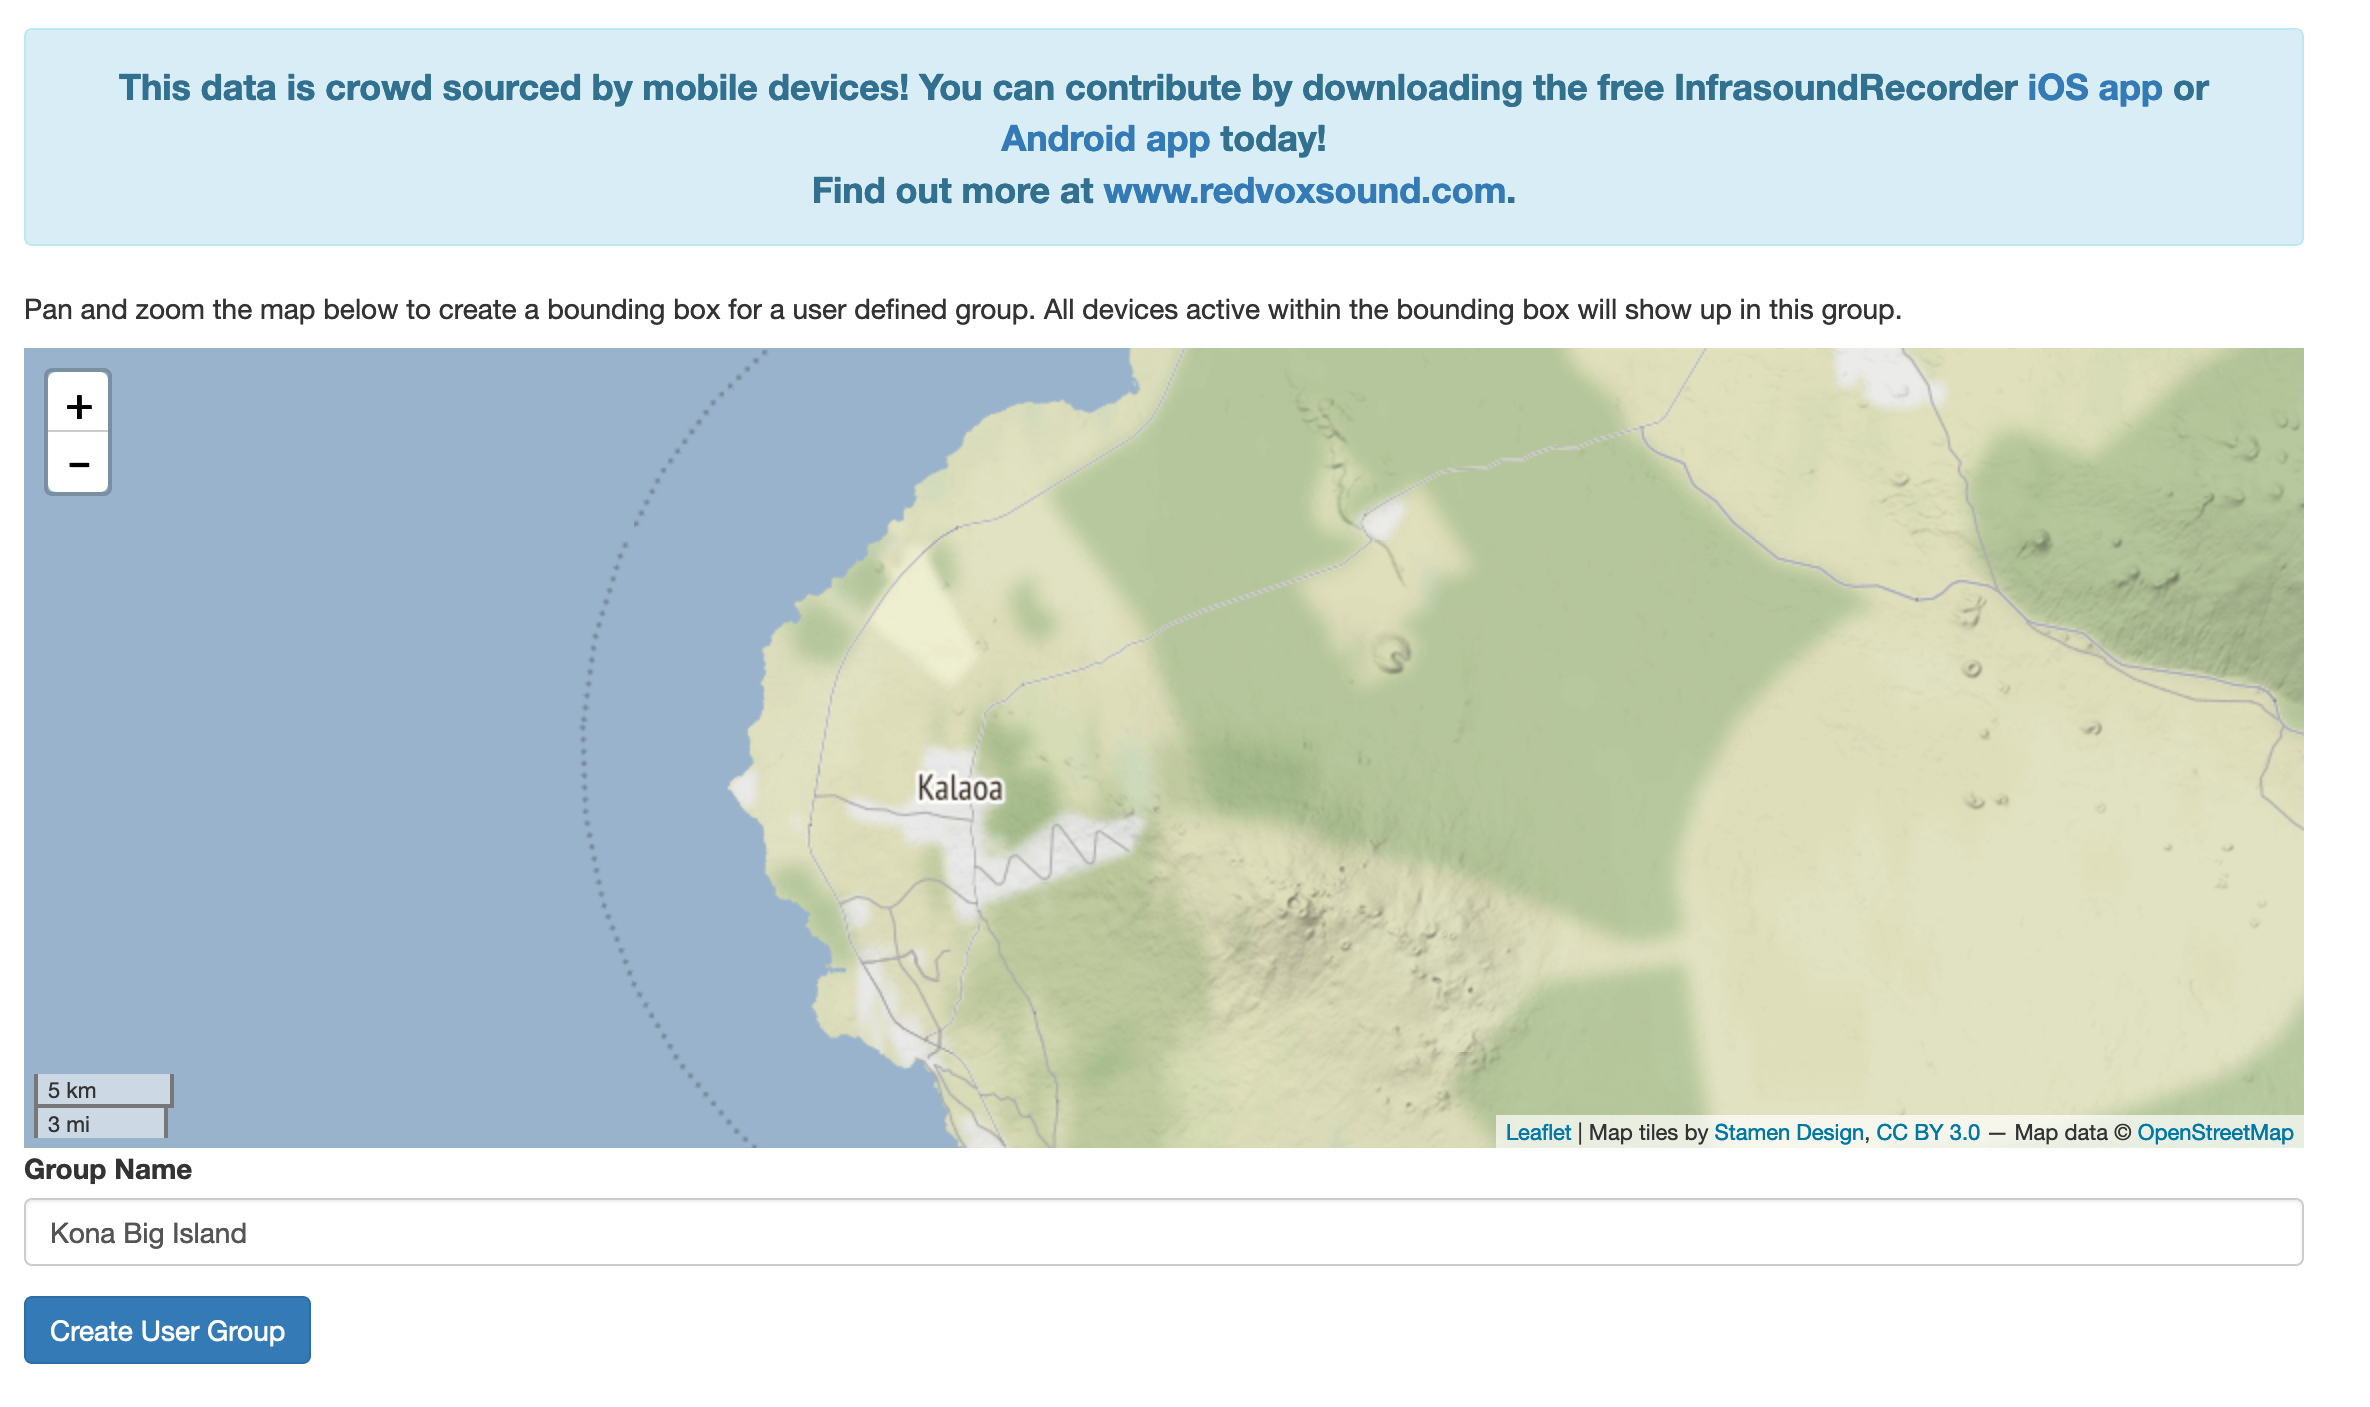
\includegraphics[width=0.7\linewidth]{figures/lweb_groupcreate.png}
	\caption{Sensor Group Creation}
	\label{fig:lweb_groupcreate}
\end{figure}

Once a group is created, you can then view the status of all devices in that group by going to the group's page. This page will display device activity for each device over the past hour and provides a quick interface for generating an analysis report from that specific grouping of devices. This data is a combination of metadata and real-time data from the Kafka buffer. An example of this is displayed in Figure~\ref{fig:lweb_group}.

\begin{figure}
	\centering
	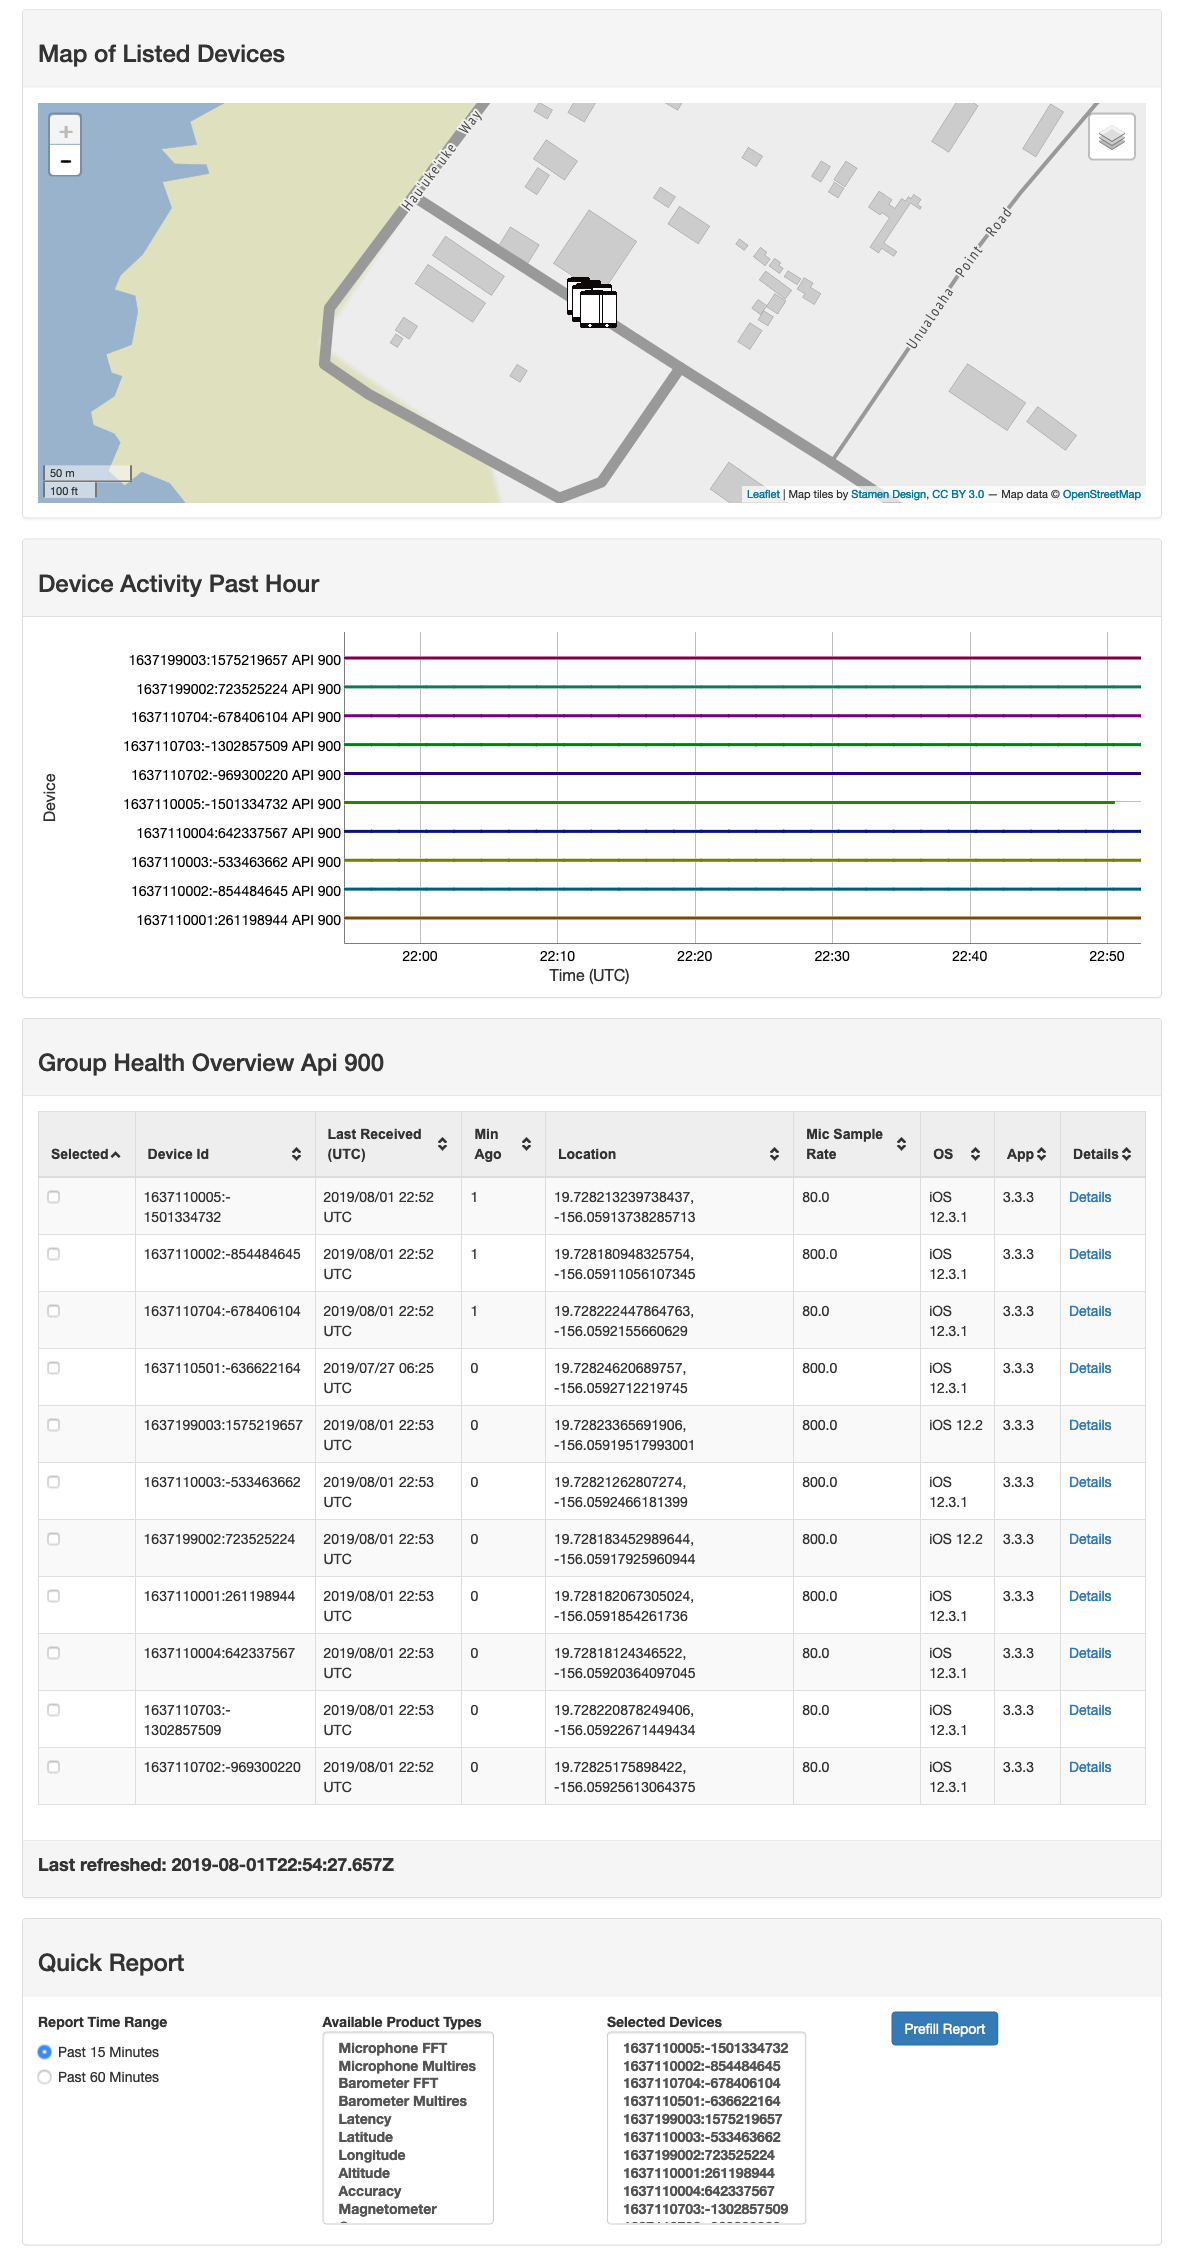
\includegraphics[width=0.65\linewidth]{figures/lweb_group.png}
	\caption{Sensor Group Status}
	\label{fig:lweb_group}
\end{figure}

\subsubsection{Data Explorer}
The ``Data Explorer" page provides a custom built interface that displays details of individual data packets as they arrive. This is useful for debugging and ensuring that the sensors are sending what the users expect the sensors to be sending.

This page displays information loaded from the database. If a sensor channel is selected, then the payload is received from AWS S3 and displayed on this page using a custom JavaScript plotter. This page also allows users to download individual data packets or export payloads as CSV\@.

An example of the data explorer is provided in Figure~\ref{fig:lweb_dataexplorer} and shows the waveform from a selected microphone channel.

\begin{figure}
	\centering
	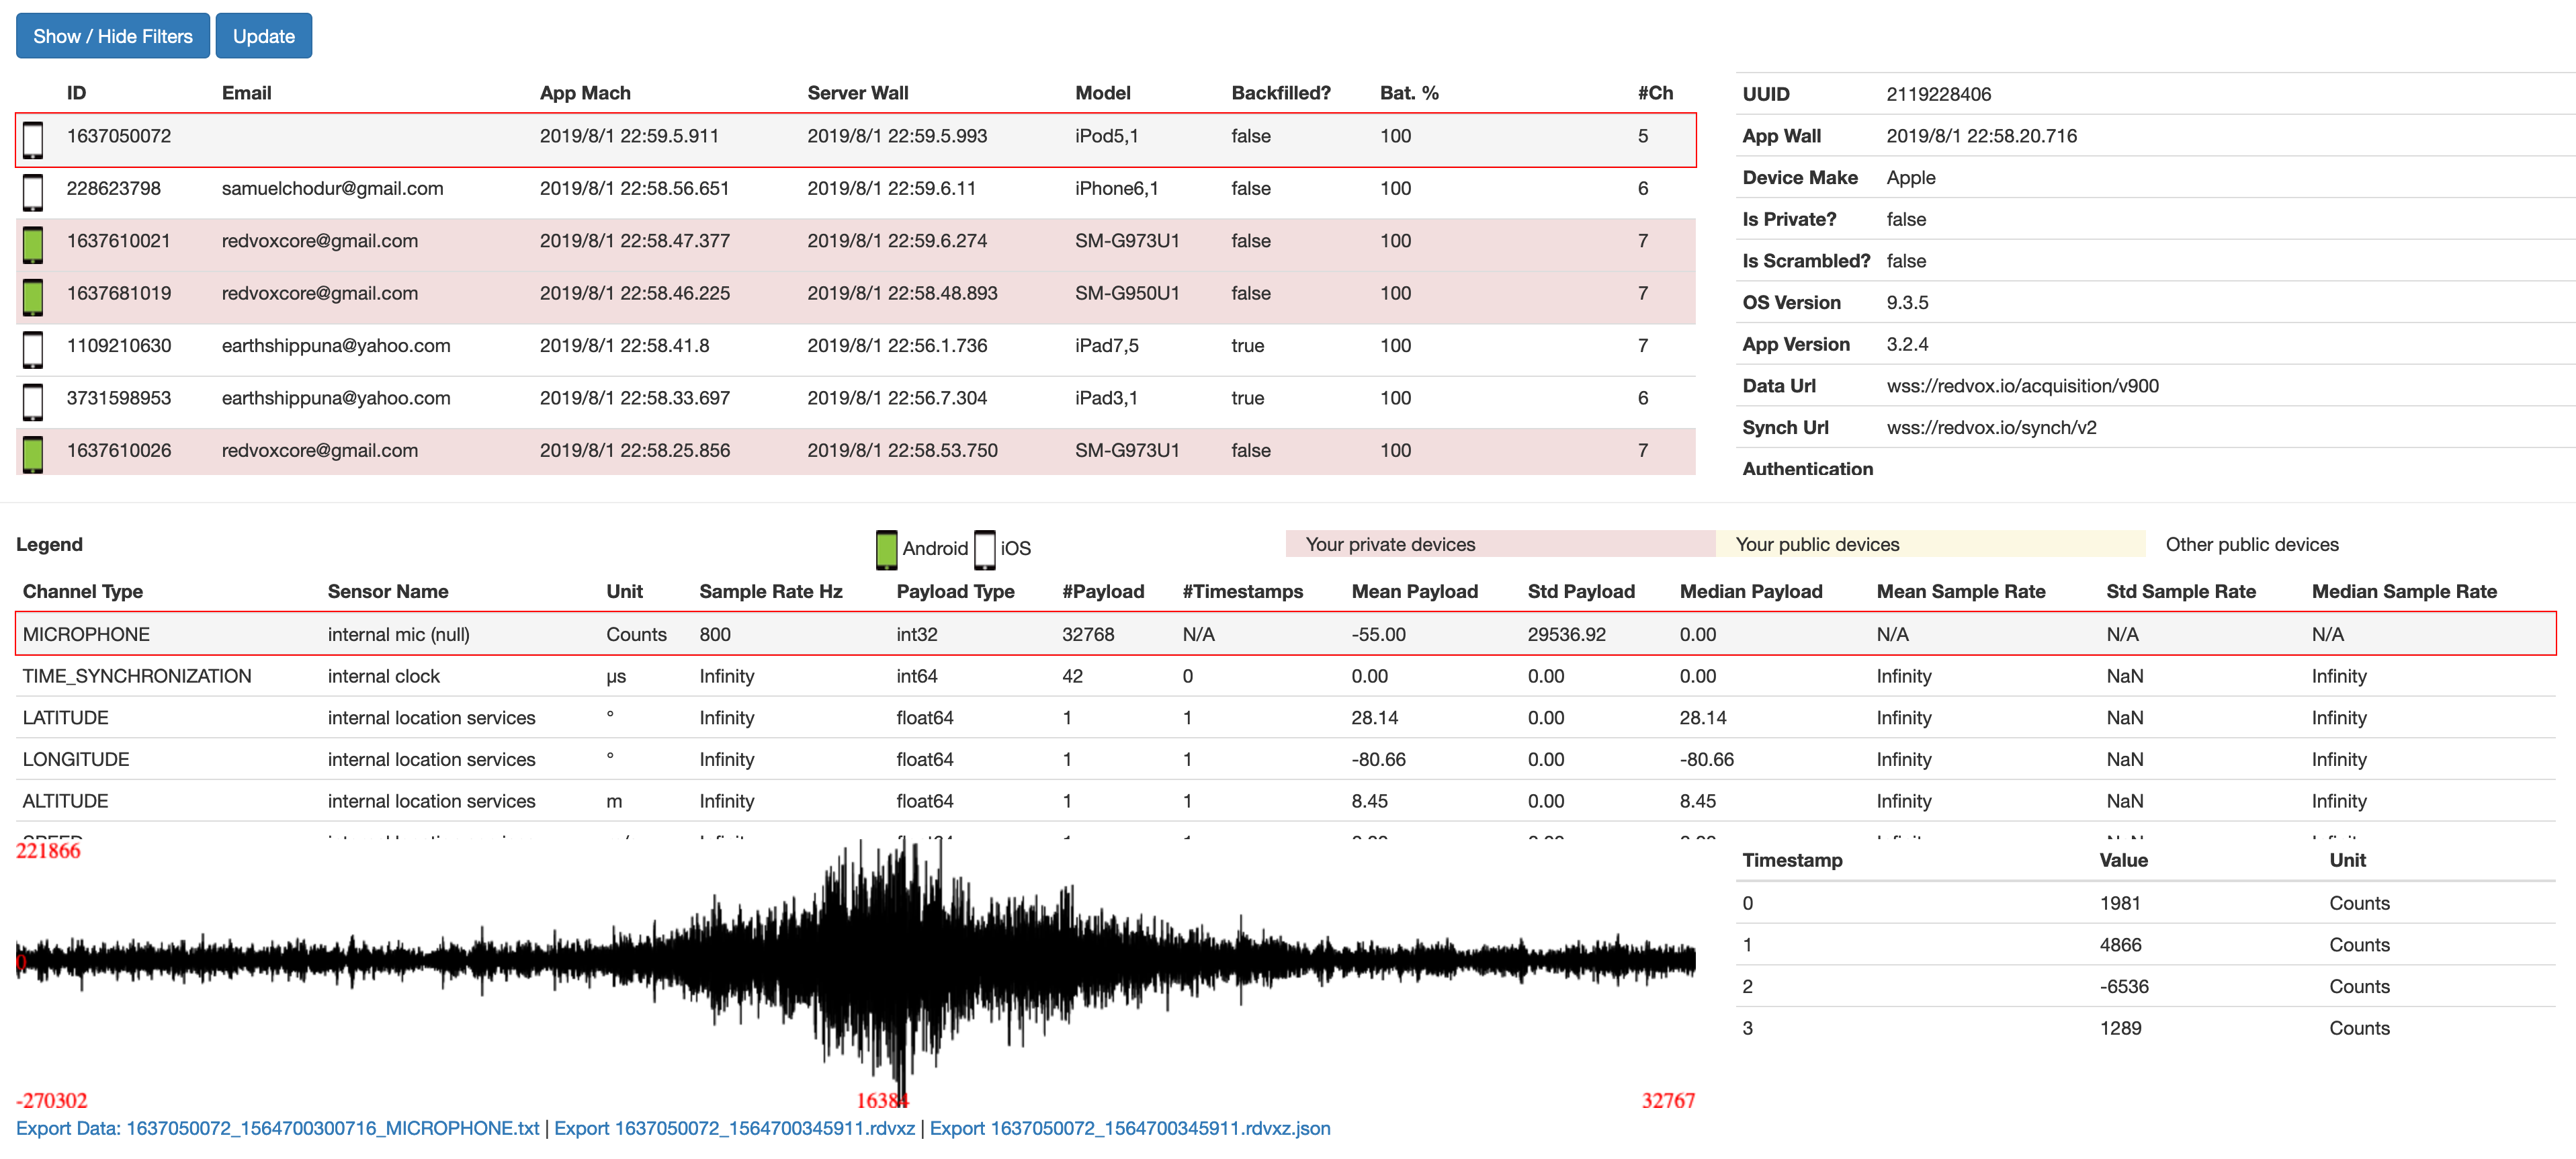
\includegraphics[width=0.7\linewidth]{figures/lweb_dataexplorer.png}
	\caption{Data Explorer Interface}
	\label{fig:lweb_dataexplorer}
\end{figure}

Data within the explorer can be filtered by device Id, device owner, time window, device make/model, os version, app version, microphone sampling rate, onboard sensors, and privacy status.

\subsubsection{Analysis Reports}
The main component of Lokahi Web is its report generation functionality. This functionality allows users to generate analysis reports from sensors that they can access with configurable time windows and sensor feature selection. Users can edit report metadata, rerun reports with new parameters, and share their reports with other Lokahi Web users. Administrators can set reports as featured reports which then make those reports available to the general public.

The report generation interface allows users to select devices, time windows, and which products should be generated. When a user selects a time window and an estimated signal source location, the interface automatically lists available sensors for that time window sorted by distance from the signal source. This makes it easy for users to determine which sensors to include in the report by seeing how far sensors are from estimated signal sources.

When a user has selected all configuration options, a report analysis request is serialized with Protocol Buffers and sent to the Lokahi Analysis service where the report is actually generated. Once the report is generated, the analysis service sends a response back to Lokahi Web and Lokahi Web displays the newly minted report.

The report interface also allows users to download raw sensor data for the selected devices over the selected time range.

An example of the report interface is provided in Figure~\ref{fig:lweb_reportcreate}.

\begin{figure}
	\centering
	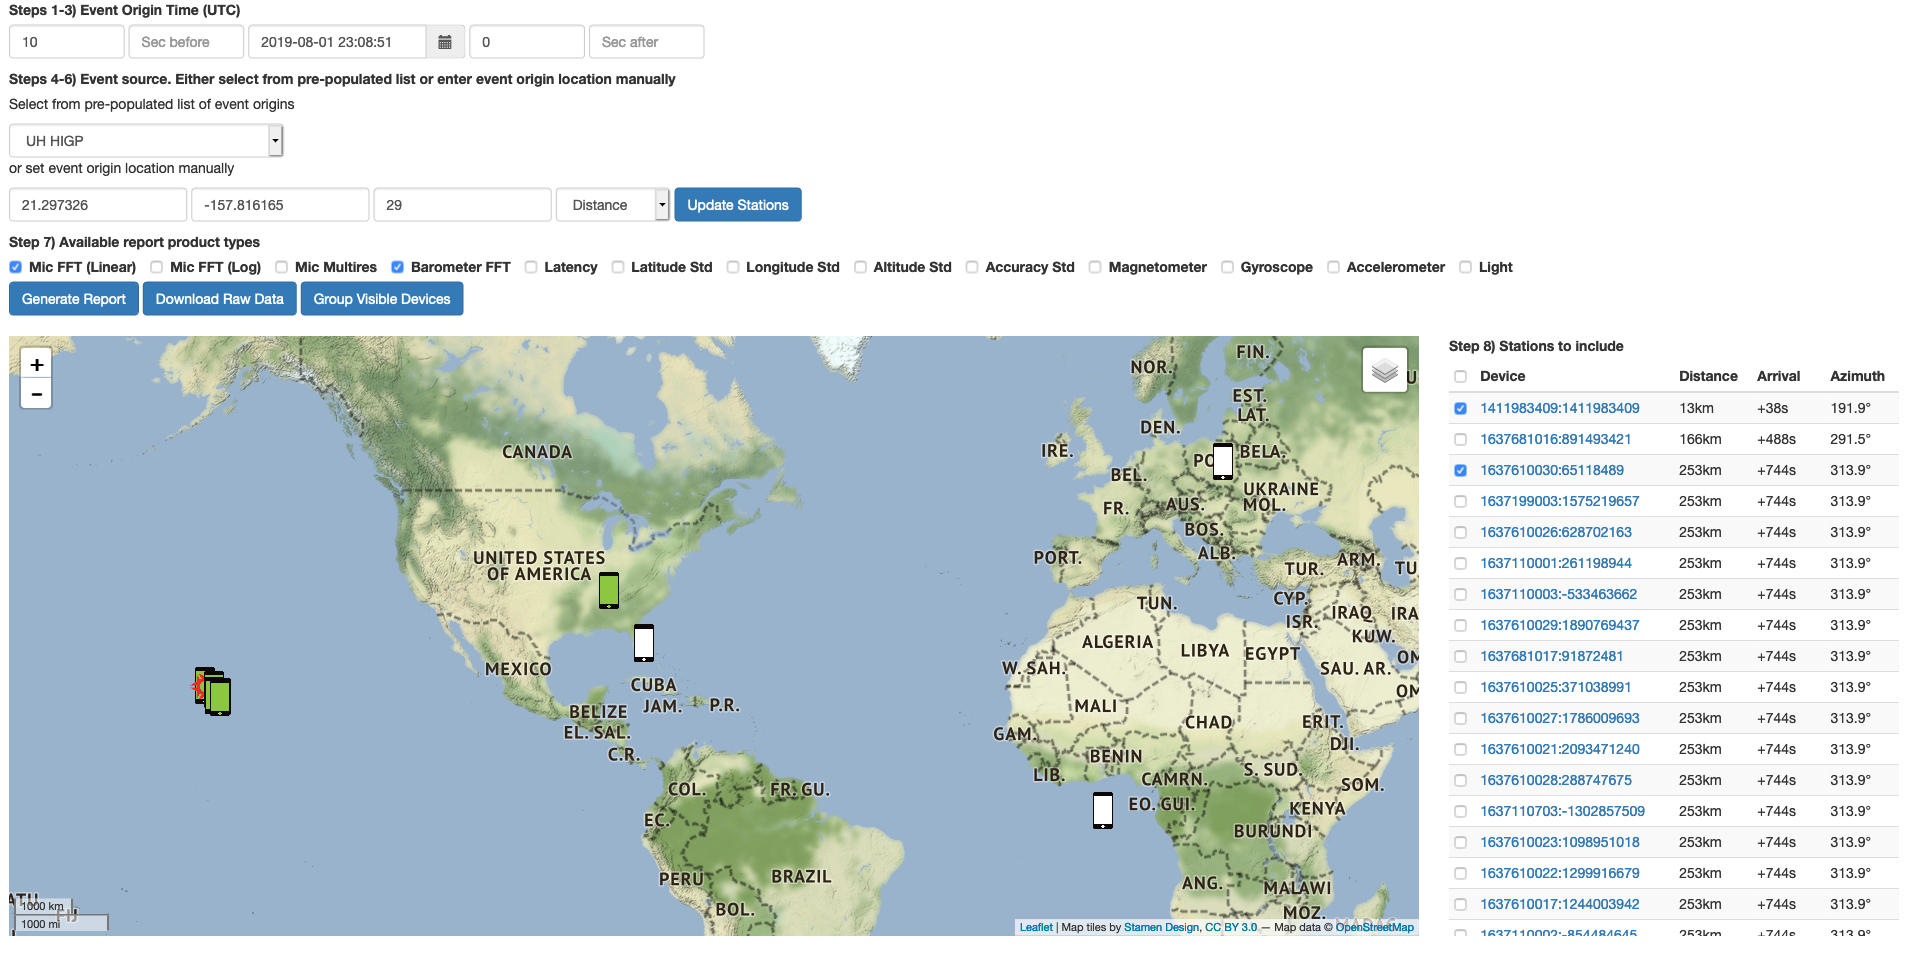
\includegraphics[width=0.7\linewidth]{figures/lweb_reportcreate.png}
	\caption{Report Creation Interface}
	\label{fig:lweb_reportcreate}
\end{figure}

An example of a report with one device is provided in Figure~\ref{fig:lweb_report}.

\begin{figure}
	\centering
	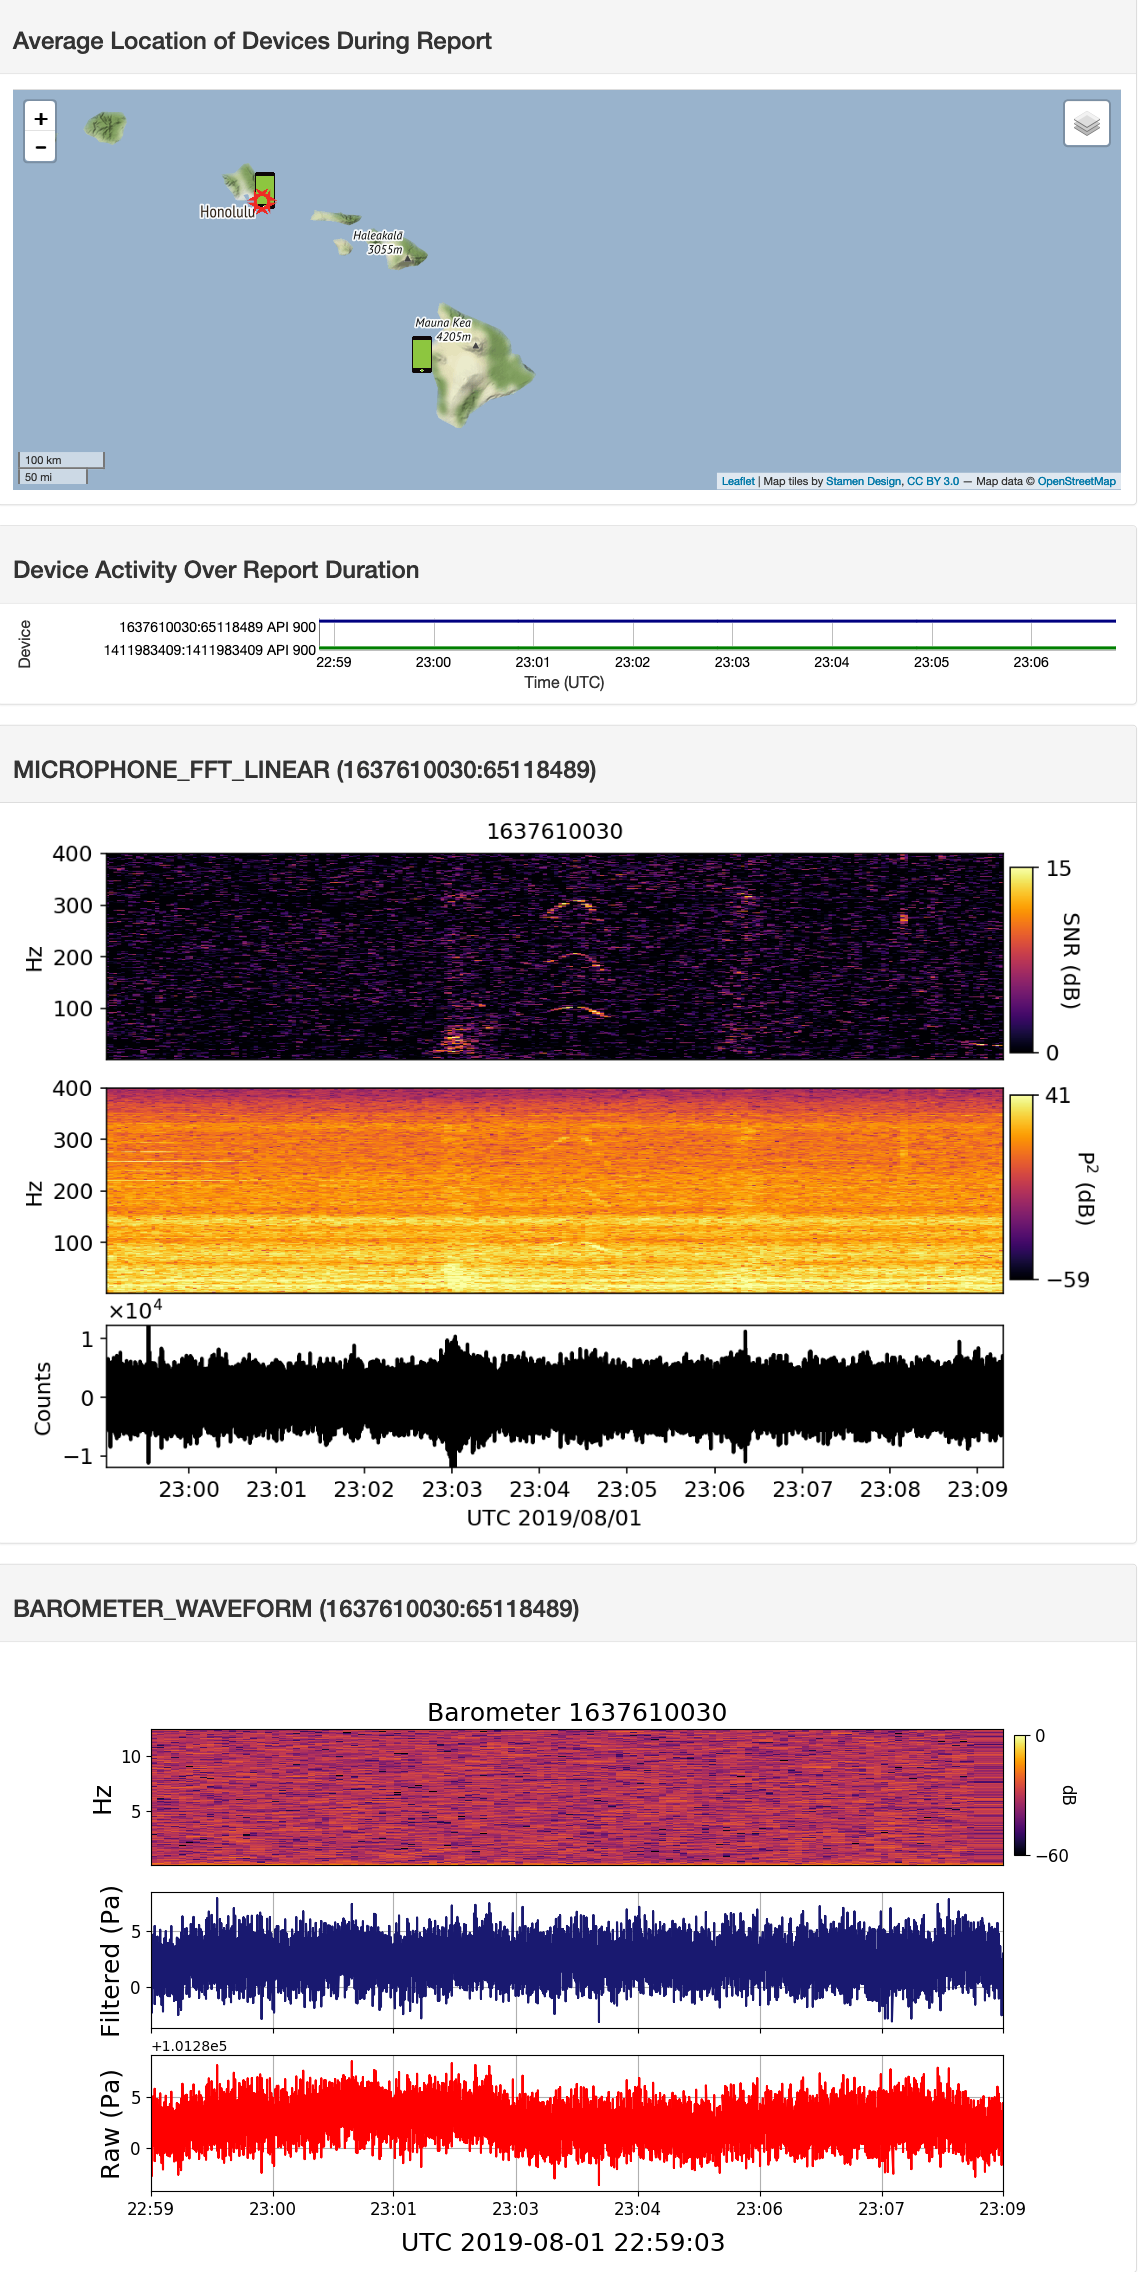
\includegraphics[width=0.6\linewidth]{figures/lweb_report.png}
	\caption{Lokahi Web Report}
	\label{fig:lweb_report}
\end{figure}

Users have the ability to sanitize reports. This removes timing, device, and location information from the reports and instead displays these values as relative offsets. For example, time is offset as seconds since 0 and location is offset as distance from an unknown source. This allows users to share sensitive reports while removing identifying information.

Each report also has a link that allows users to download the raw sensor data that was used in generating the report.

The metadata of each report can also be directly edited. This includes adding Annotation Phenomena to classified Incidents. This is fundamental for Lokahi's goals of building up a labeled dataset for future machine learning endeavors.

Finally, there is a ``Print Version" interface of reports that removes some of the metadata, rearranges the maps and plots for printing or distribution.

\subsubsection{Global Collection}
The global collection interface shows the last location of every device that Lokahi has ever received. This interface is useful for showing sensor deployment adoption. This interface is shown in Figure~\ref{fig:lweb_global}.

\begin{figure}
	\centering
	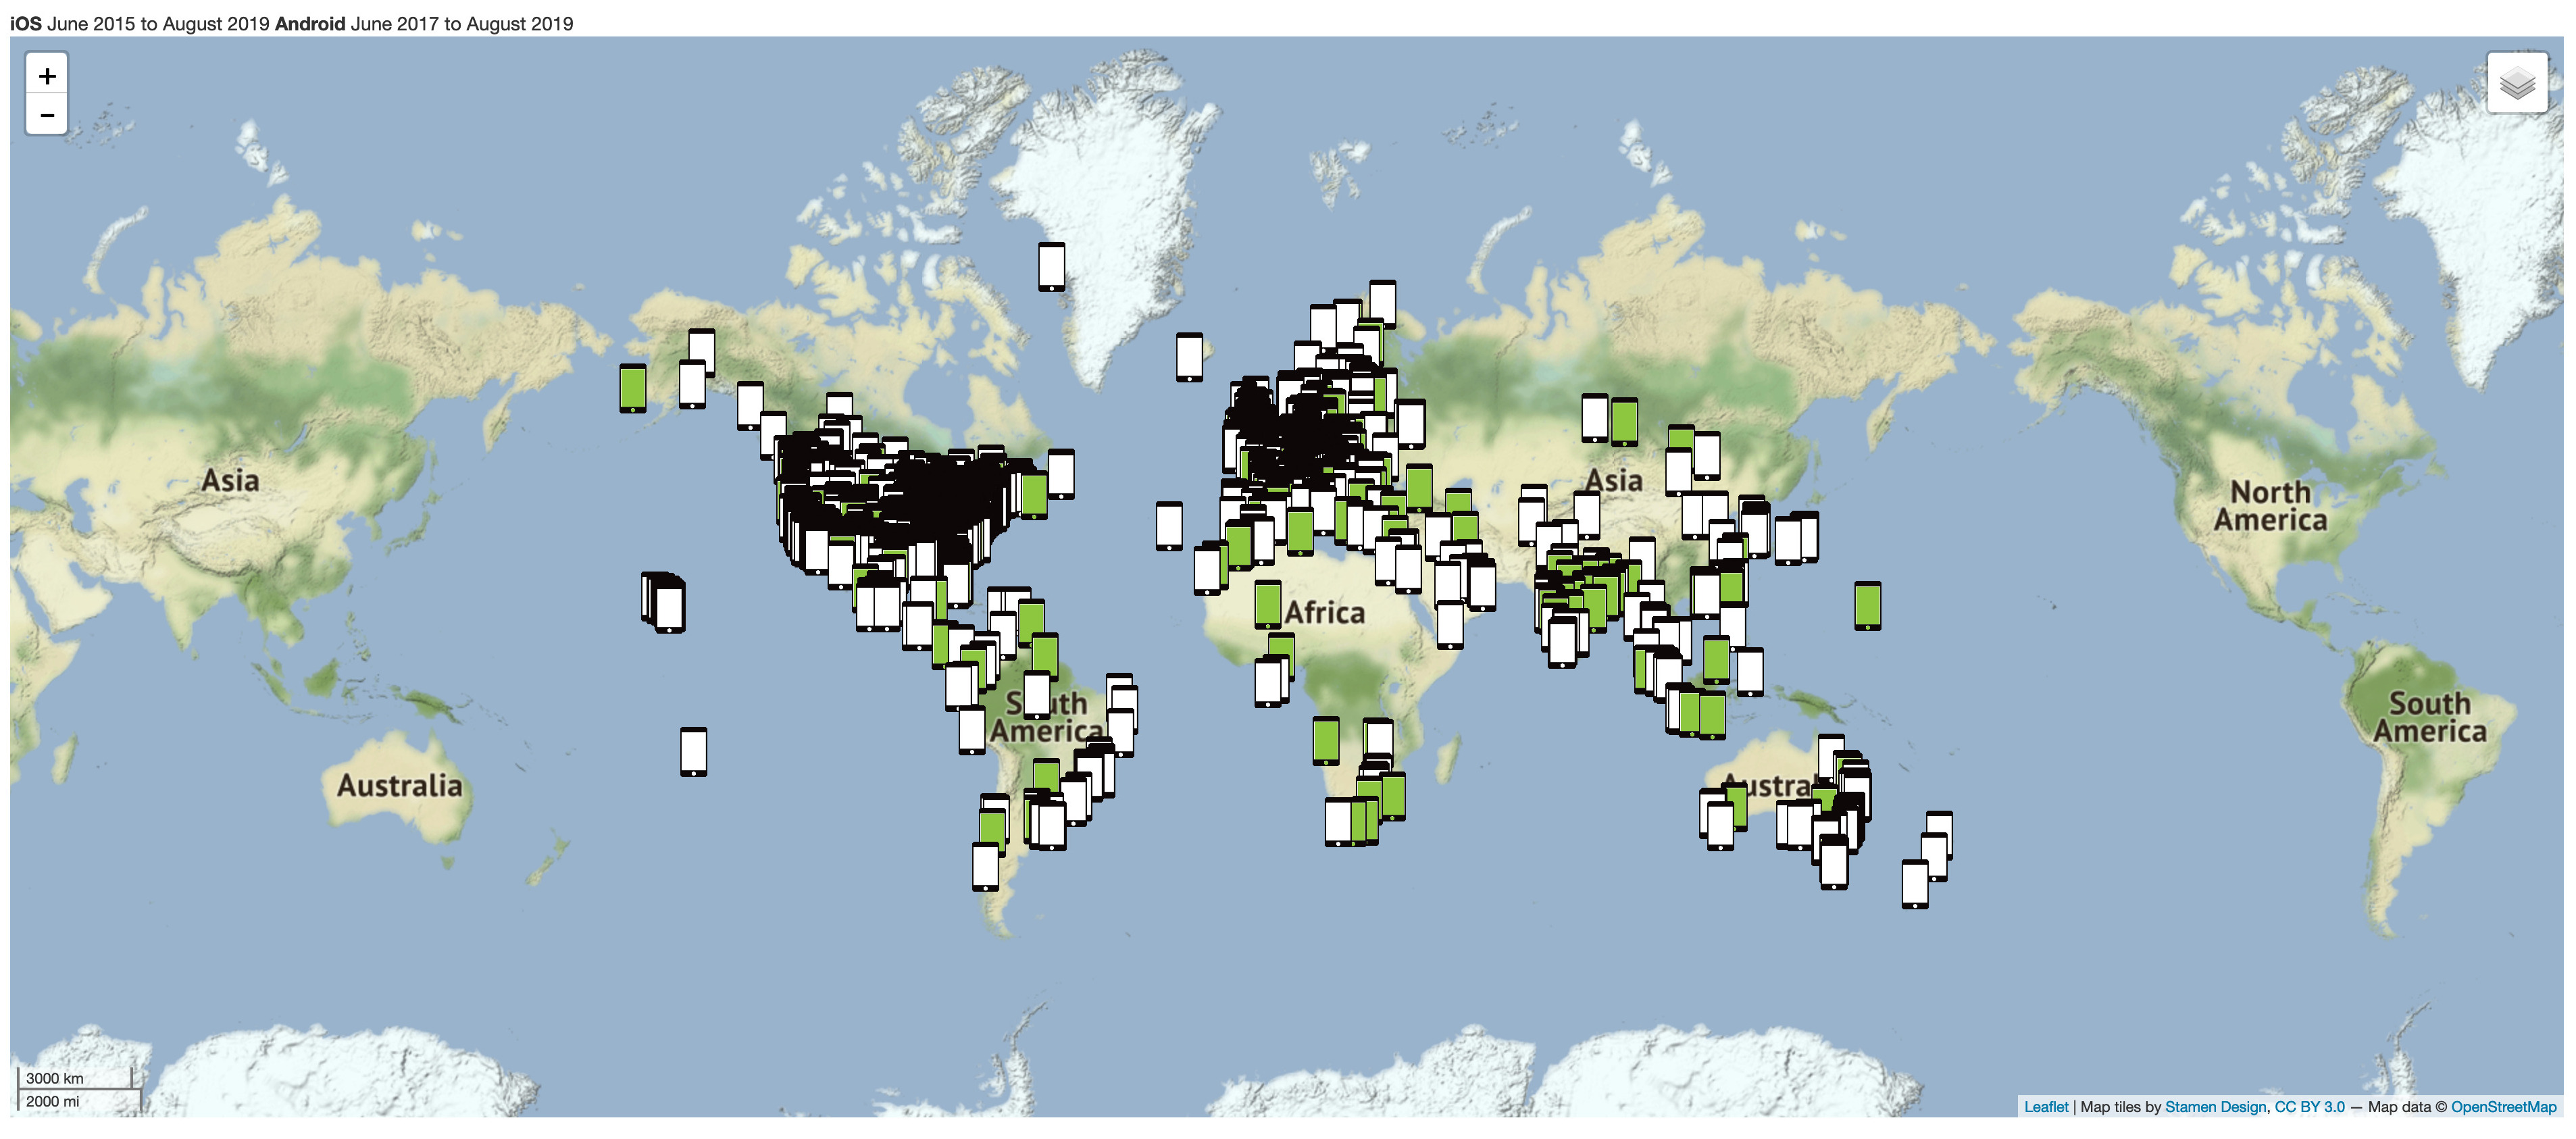
\includegraphics[width=0.7\linewidth]{figures/lweb_global.jpg}
	\caption{Lokahi Global Collection}
	\label{fig:lweb_global}
\end{figure}

\subsubsection{Lokahi Geofenced Alerts}
Lokahi utilizes Google's Firebase Cloud Messaging (FCM) to send geofenced alerts to mobile devices. Since we know the location of each device through its metadata, it is possible to define a bounding box in which only devices within that bounding box will receive an alert.

This is useful when we want to alert users of our sensors to specific events and provides a means of producing actionable insights that can increase S2N. As an example, we may wan to collect data on an upcoming SpaceX launch in Florida. We can create a bounding box for all users in the target area and alert them to an upcoming launch and ask them to turn on their sensors for data collection.

The interface for this is provided by ``Lokahi Web". Once an administrator selects their bounding box and supplies their alert message, Lokahi Web uses the FCM API for queuing a message to all sensors in the target area.

An example of the alerting interface is provided in Figure~\ref{fig:fcm}.

\begin{figure}
	\centering
	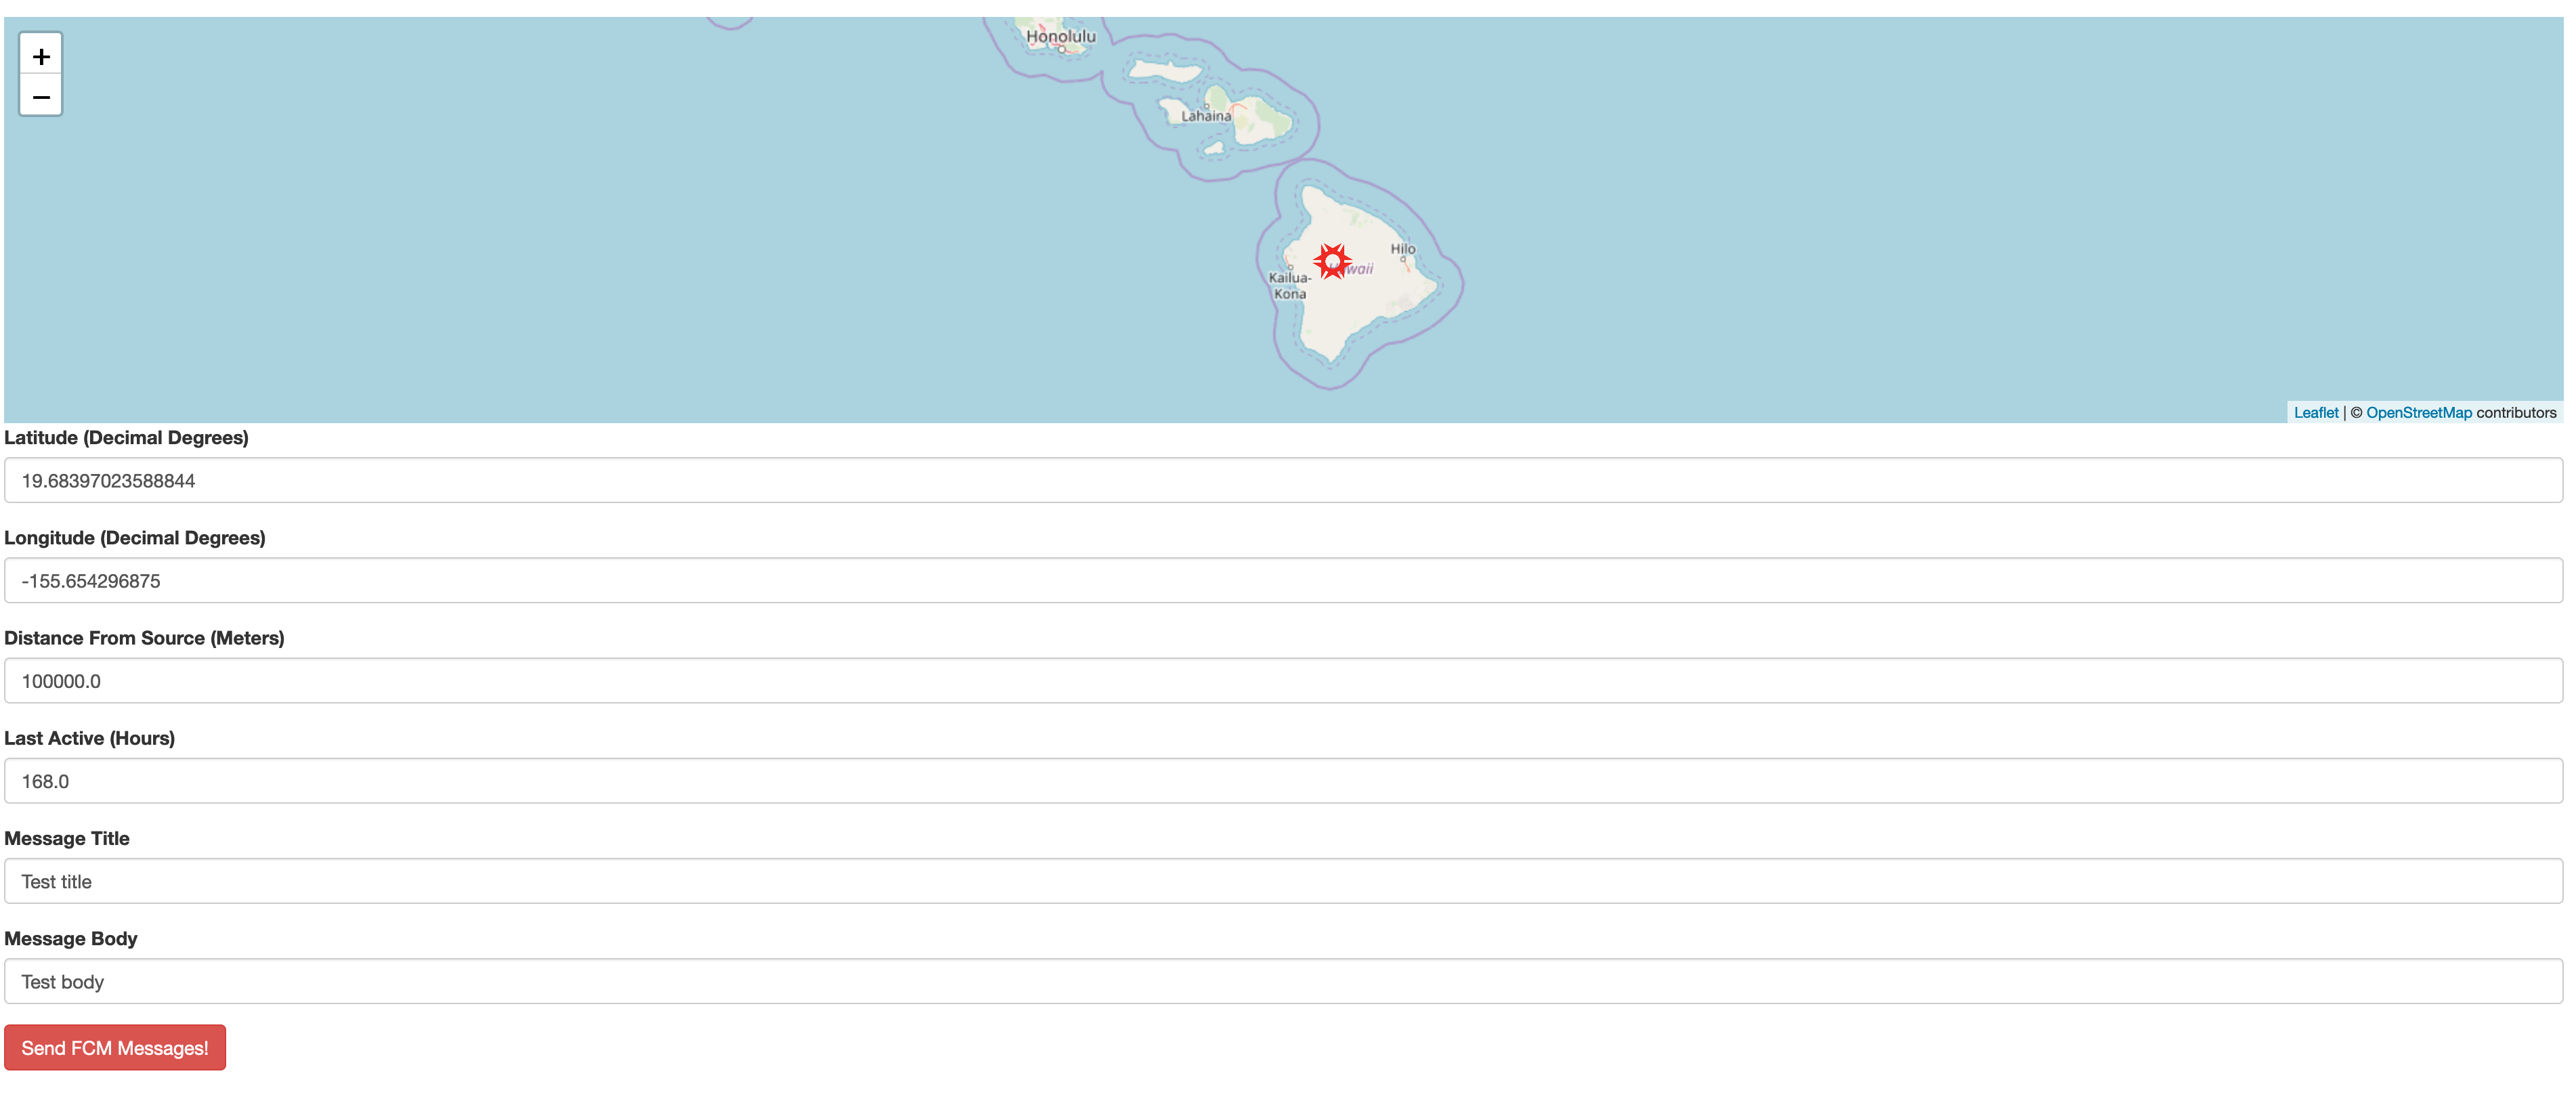
\includegraphics[width=\linewidth]{figures/fcm.png}
	\caption{Geofence Alert Interface}
	\label{fig:fcm}
\end{figure}

\chapter{Evaluation}\label{ch:evaluation}
Evaluation of the Laha framework involves deploying reference Laha-compliant DSNs, validating the data collected from the reference implementations, and then comparing and contrasting various metrics for each of the stated goals. Metrics were collected during a set of experiments for each of the Laha reference implementations in summer 2019.

The following sections describe my approach to deploying the reference implementations, data validation, evaluating the main goals of the Laha framework, and evaluating the tertiary goals of the Laha framework.

\section{Deploy Laha reference implementations on test sites}\label{sec:deploy-laha-reference-implementations-on-test-sites}
Both the OPQ and Lokahi reference implementations were deployed to test sites where validated data collection took place. The following sections describe the reference implementation deployments in detail.

\subsection{OPQ Reference Deployment}\label{subsec:opq-reference-deployment}
Fifteen Laha-compliant OPQ Boxes were deployed over the UH Manoa microgrid during the Summer and Fall of 2019.

The placement strategy I utilized aimed to maximize our ability to collect distributed PQ Events by placing sensors on the same electrical lines. We also considered placing Boxes in locations co-located with sensitive or demanding electrical equipment in the hope of seeing PQ Events generated from this equipment. Finally, we considered data access in terms of network availability and ground truth availability. Working with my colleagues and the Office of Energy Management, I selected the 15 locations for the campus wide deployment. Table~\ref{table:OpqDeployment} displays the details of the UH Manoa campus deployment and justifications for choosing those locations.

\begin{table}[H]
	\centering
	\caption{OPQ Deployment}
	\begin{tabularx}{\textwidth}{lllX}
		\toprule
		\textbf{Box} & \textbf{Location} & \textbf{Latitude} & \textbf{Longitude} \\
		\midrule
		1000 & POST 1 & -157.816237 & 21.297438 \\
		1001 & Hamilton & -157.816173 & 21.300332 \\
		1002 & POST 2 & -157.816305 & 21.297663 \\
		1003 & LAVA Lab & -157.816034748669 & 21.29974948387028 \\
		1005 & Parking Structure Ph II & -157.819234 & 21.296042 \\
		1006 & Frog 1 & -157.823122 & 21.29805 \\
		1007 & Frog 2 & -157.822819 & 21.298046 \\
		1008 & Mile's Office & -157.8137681609306 & 21.30386147625208 \\
		1009 & Watanabe & -157.815817 & 21.298351 \\
		1010 & Holmes & -157.816104 & 21.297011 \\
		1021 & Marine Science Building & -157.8156900462205 & 21.29789461271471 \\
		1022 & Ag. Engineering & -157.8154874938278 & 21.30163608338939 \\
		1023 & Law Library & -157.817361 & 21.296328 \\
		1024 & IT Building & -157.816451 & 21.29886 \\
		1025 & Kennedy Theater & -157.815225 & 21.299282 \\
		\bottomrule
	\end{tabularx}
	\label{table:OpqDeployment}
\end{table}

Determination of electrical lines was aided by the UH Manoa electrical blueprint as displayed in Figure~\ref{fig:UhGridTopo}.

\begin{figure}[H]
	\centering
	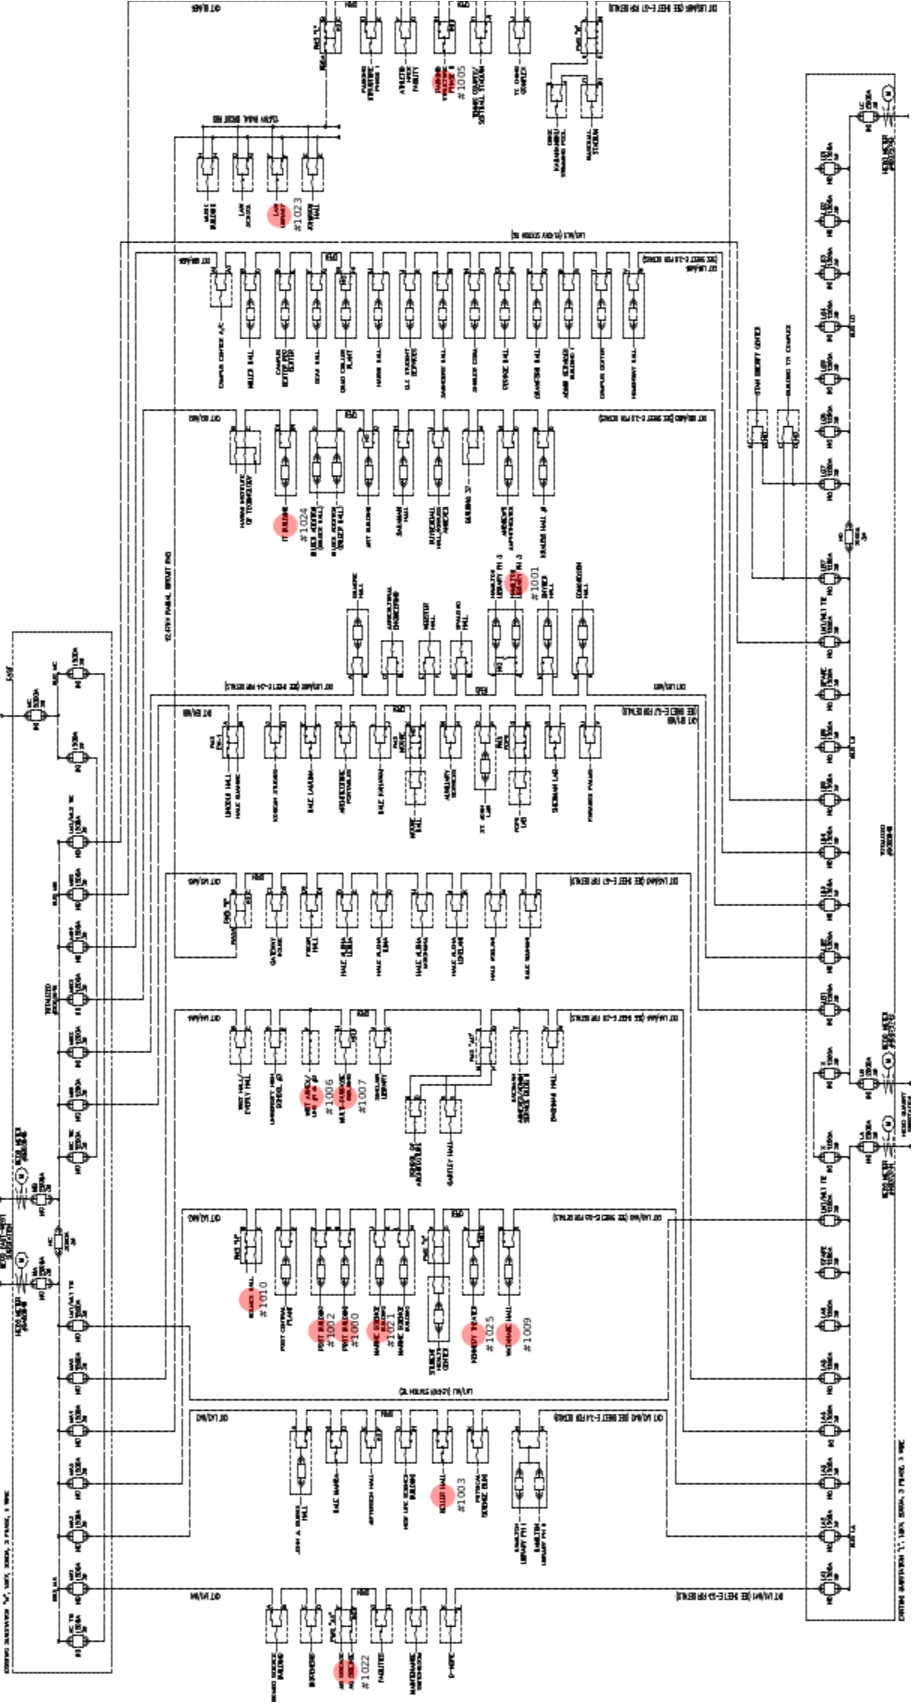
\includegraphics[height=\textheight]{figures/uh_power_grid.pdf}
	\caption{UH Deployment Grid Topology}
	\label{fig:UhGridTopo}
\end{figure}

A graphical representation showing the complete coverage of Boxes on the UH Manoa microgrid is displayed in Figure~\ref{fig:UhDeploy}.

\begin{figure}[H]
	\centering
	\includegraphics[width=\linewidth]{figures/deploy.jpg}
	\caption{UH Deployment}
	\label{fig:UhDeploy}
\end{figure}

All devices were placed in a location that had access to UH Manoa's wireless network. As soon as they were installed, they started transmitting PQ data for that location.

\subsection{Lokahi Deployment}\label{subsec:lokahi-deployment}

Over a period of three months, data was collected from over 100 Lokahi sensors at large distributed globally.

Figure~\ref{fig:active_lokahi_sensors_i} shows the number of active Lokahi sensors sampling at different sampling rates over this period.

\begin{figure}[H]
	\centering
	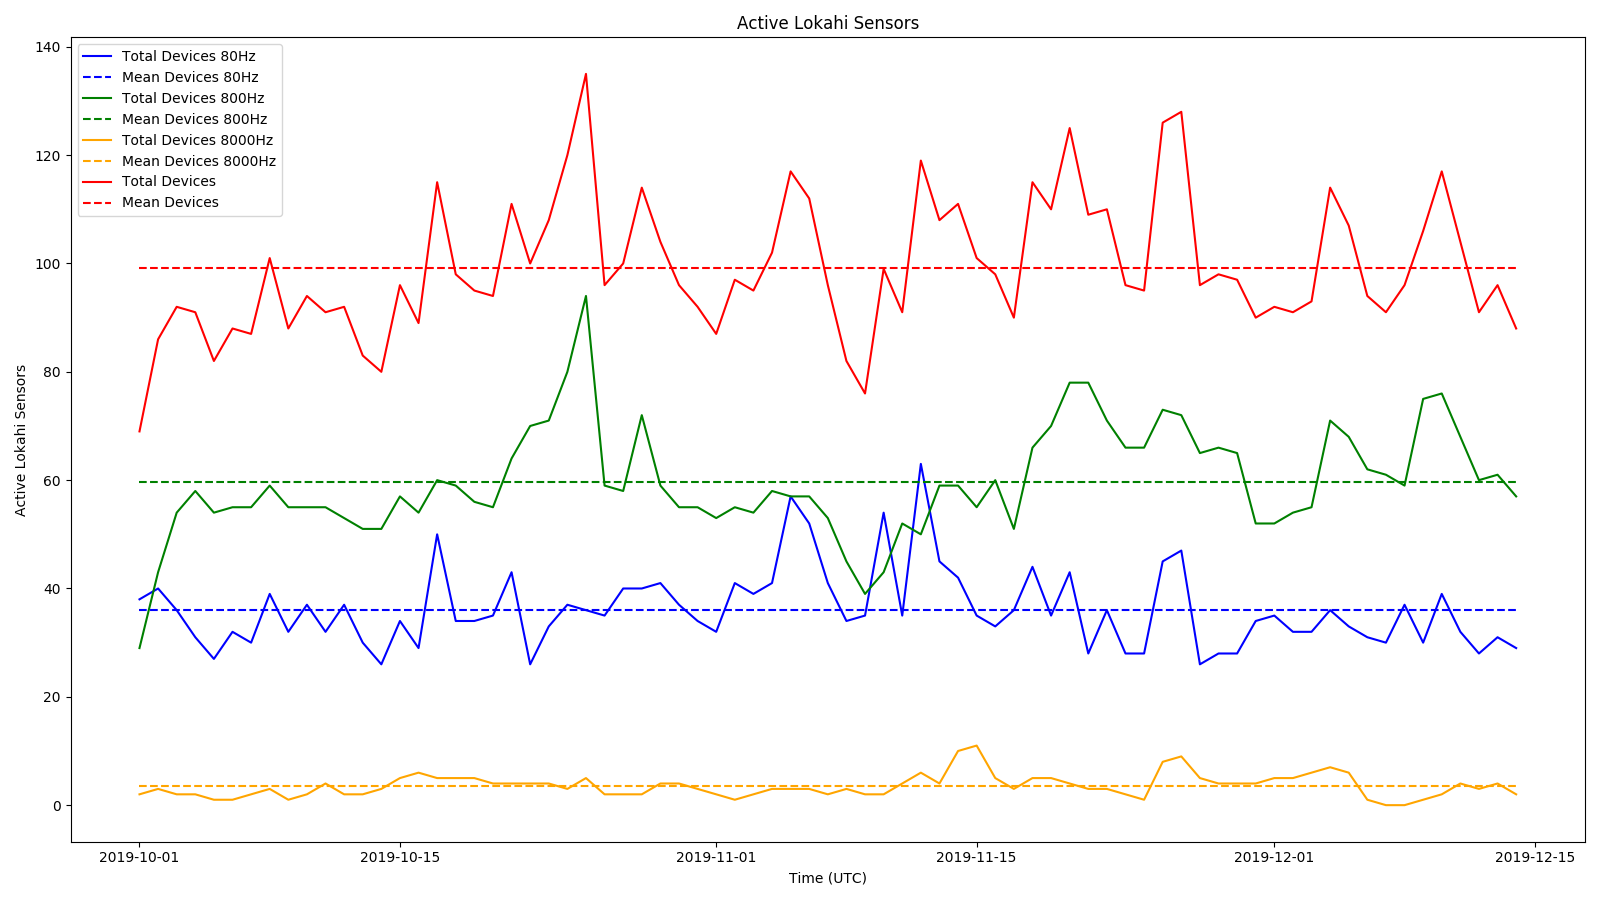
\includegraphics[width=\linewidth]{figures/lokahi_num_sensors.png}
	\caption{Active Lokahi Sensors}
	\label{fig:active_lokahi_sensors_i}
\end{figure}

Data was collected globally. The next series of Figures will show where data was collected from using the Lokahi network over the deployment window. It should be noted that this map only displays data from sensors that recorded public data. This was done to protect the privacy of users that have marked their data as private. Other results for the Lokahi network utilize the full data set of public and private data. I took care to not expose any private details and only provide results as statistical summaries.

Figure~\ref{fig:lokahi_deploy_1} shows Lokahi sensors deployed in the state of Hawaii.

\begin{figure}[H]
	\centering
	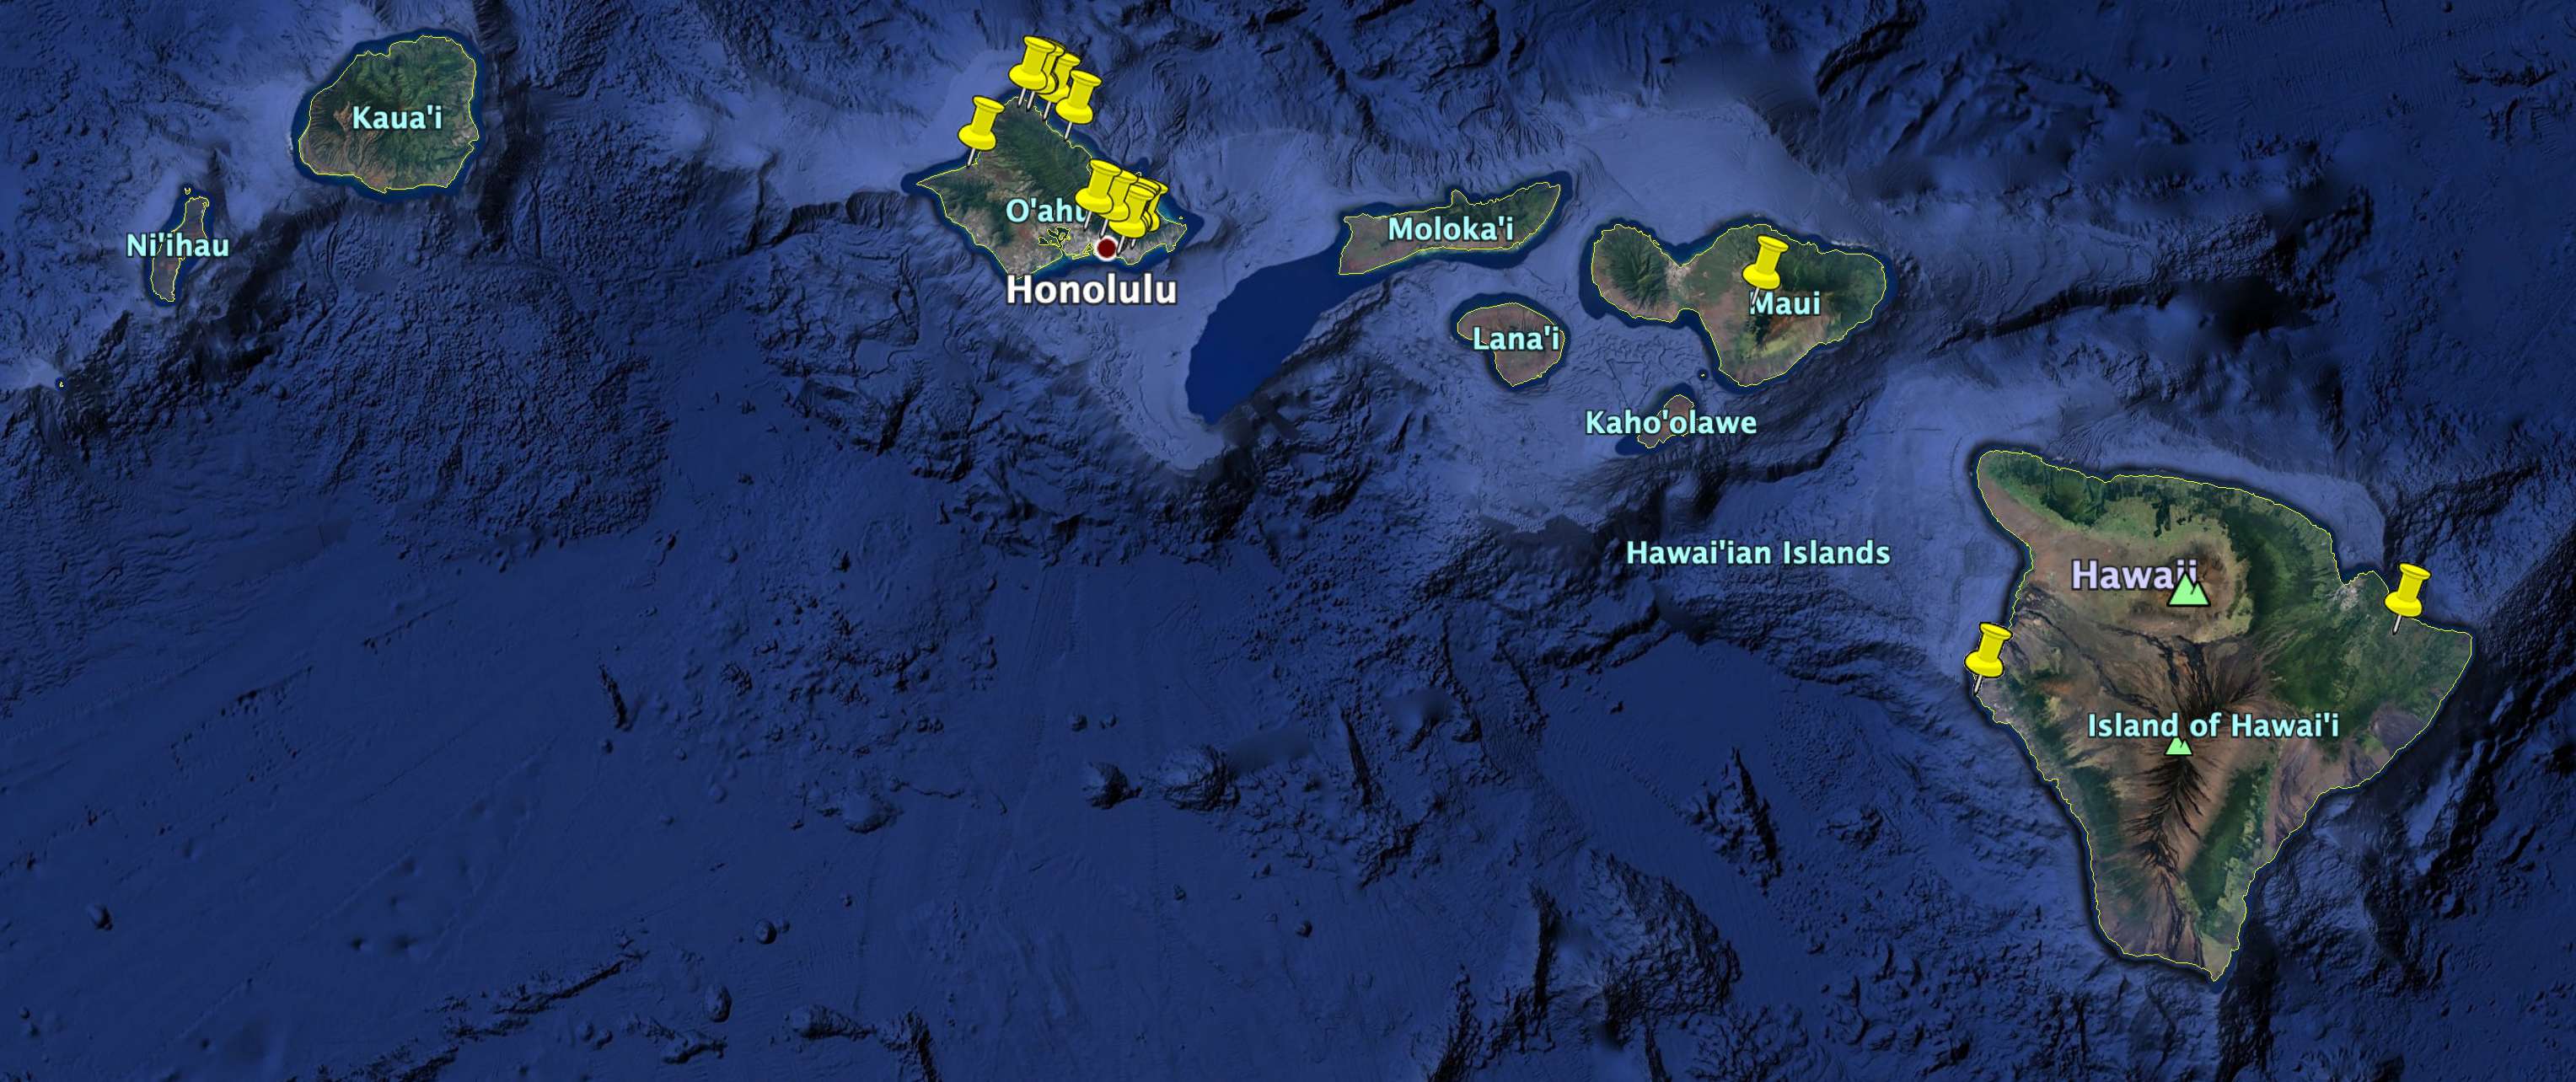
\includegraphics[width=\linewidth]{figures/lokahi_deploy_1.jpg}
	\caption{Lokahi Sensors: Hawaii}
	\label{fig:lokahi_deploy_1}
\end{figure}

Here, we can observe sensor coverage on the islands of Oahu, Maui, and the Big Island of Hawaii.

Figure~\ref{fig:lokahi_deploy_2} shows Lokahi sensors deployed across North America.

\begin{figure}[H]
	\centering
	\includegraphics[width=\linewidth]{figures/lokahi_deploy_2.jpg}
	\caption{Lokahi Sensors: North America}
	\label{fig:lokahi_deploy_2}
\end{figure}

Lokahi has provided significant sensor coverage over the North American continent with most sensors located in the United States and others located in Mexico and Canada.

Figure~\ref{fig:lokahi_deploy_3} shows Lokahi sensors deployed through Central and South America.

\begin{figure}[H]
	\centering
	\includegraphics[width=\linewidth]{figures/lokahi_deploy_3.jpg}
	\caption{Lokahi Sensors: Central and South America}
	\label{fig:lokahi_deploy_3}
\end{figure}

Here we can see sensors that were deployed in Columbia, Costa Rica, and Brazil.

Figure~\ref{fig:lokahi_deploy_4} shows Lokahi sensors deployed through Europe and Western Asia.

\begin{figure}[H]
	\centering
	\includegraphics[width=\linewidth]{figures/lokahi_deploy_4.jpg}
	\caption{Lokahi Sensors: Europe and Western Asia}
	\label{fig:lokahi_deploy_4}
\end{figure}

Europe also provides excellent coverage for the Lokahi network. You will also note that Lokahi sensors have been deployed to several countries outside of Europe including Turkey, Israel, Ukraine, and Russia.

Figure~\ref{fig:lokahi_deploy_5} shows Lokahi sensors deployed through South-East Asia.

\begin{figure}[H]
	\centering
	\includegraphics[width=\linewidth]{figures/lokahi_deploy_5.jpg}
	\caption{Lokahi Sensors: India and South-East Asia}
	\label{fig:lokahi_deploy_5}
\end{figure}

Here, we can see Lokahi sensors that have been deployed in India, Bangladesh, Sri Lanka, Pakistan, and Malaysia.

Figure~\ref{fig:lokahi_deploy_6} shows Lokahi sensors deployed through Oceania.

\begin{figure}[H]
	\centering
	\includegraphics[width=\linewidth]{figures/lokahi_deploy_6.jpg}
	\caption{Lokahi Sensors: Oceania}
	\label{fig:lokahi_deploy_6}
\end{figure}

Lokahi sensors have been deployed to the Western, Southern, and Eastern coasts of Australia as well as New Zealand.

Figure~\ref{fig:lokahi_deploy_7} shows Lokahi sensors deployed through East Asia.

\begin{figure}[H]
	\centering
	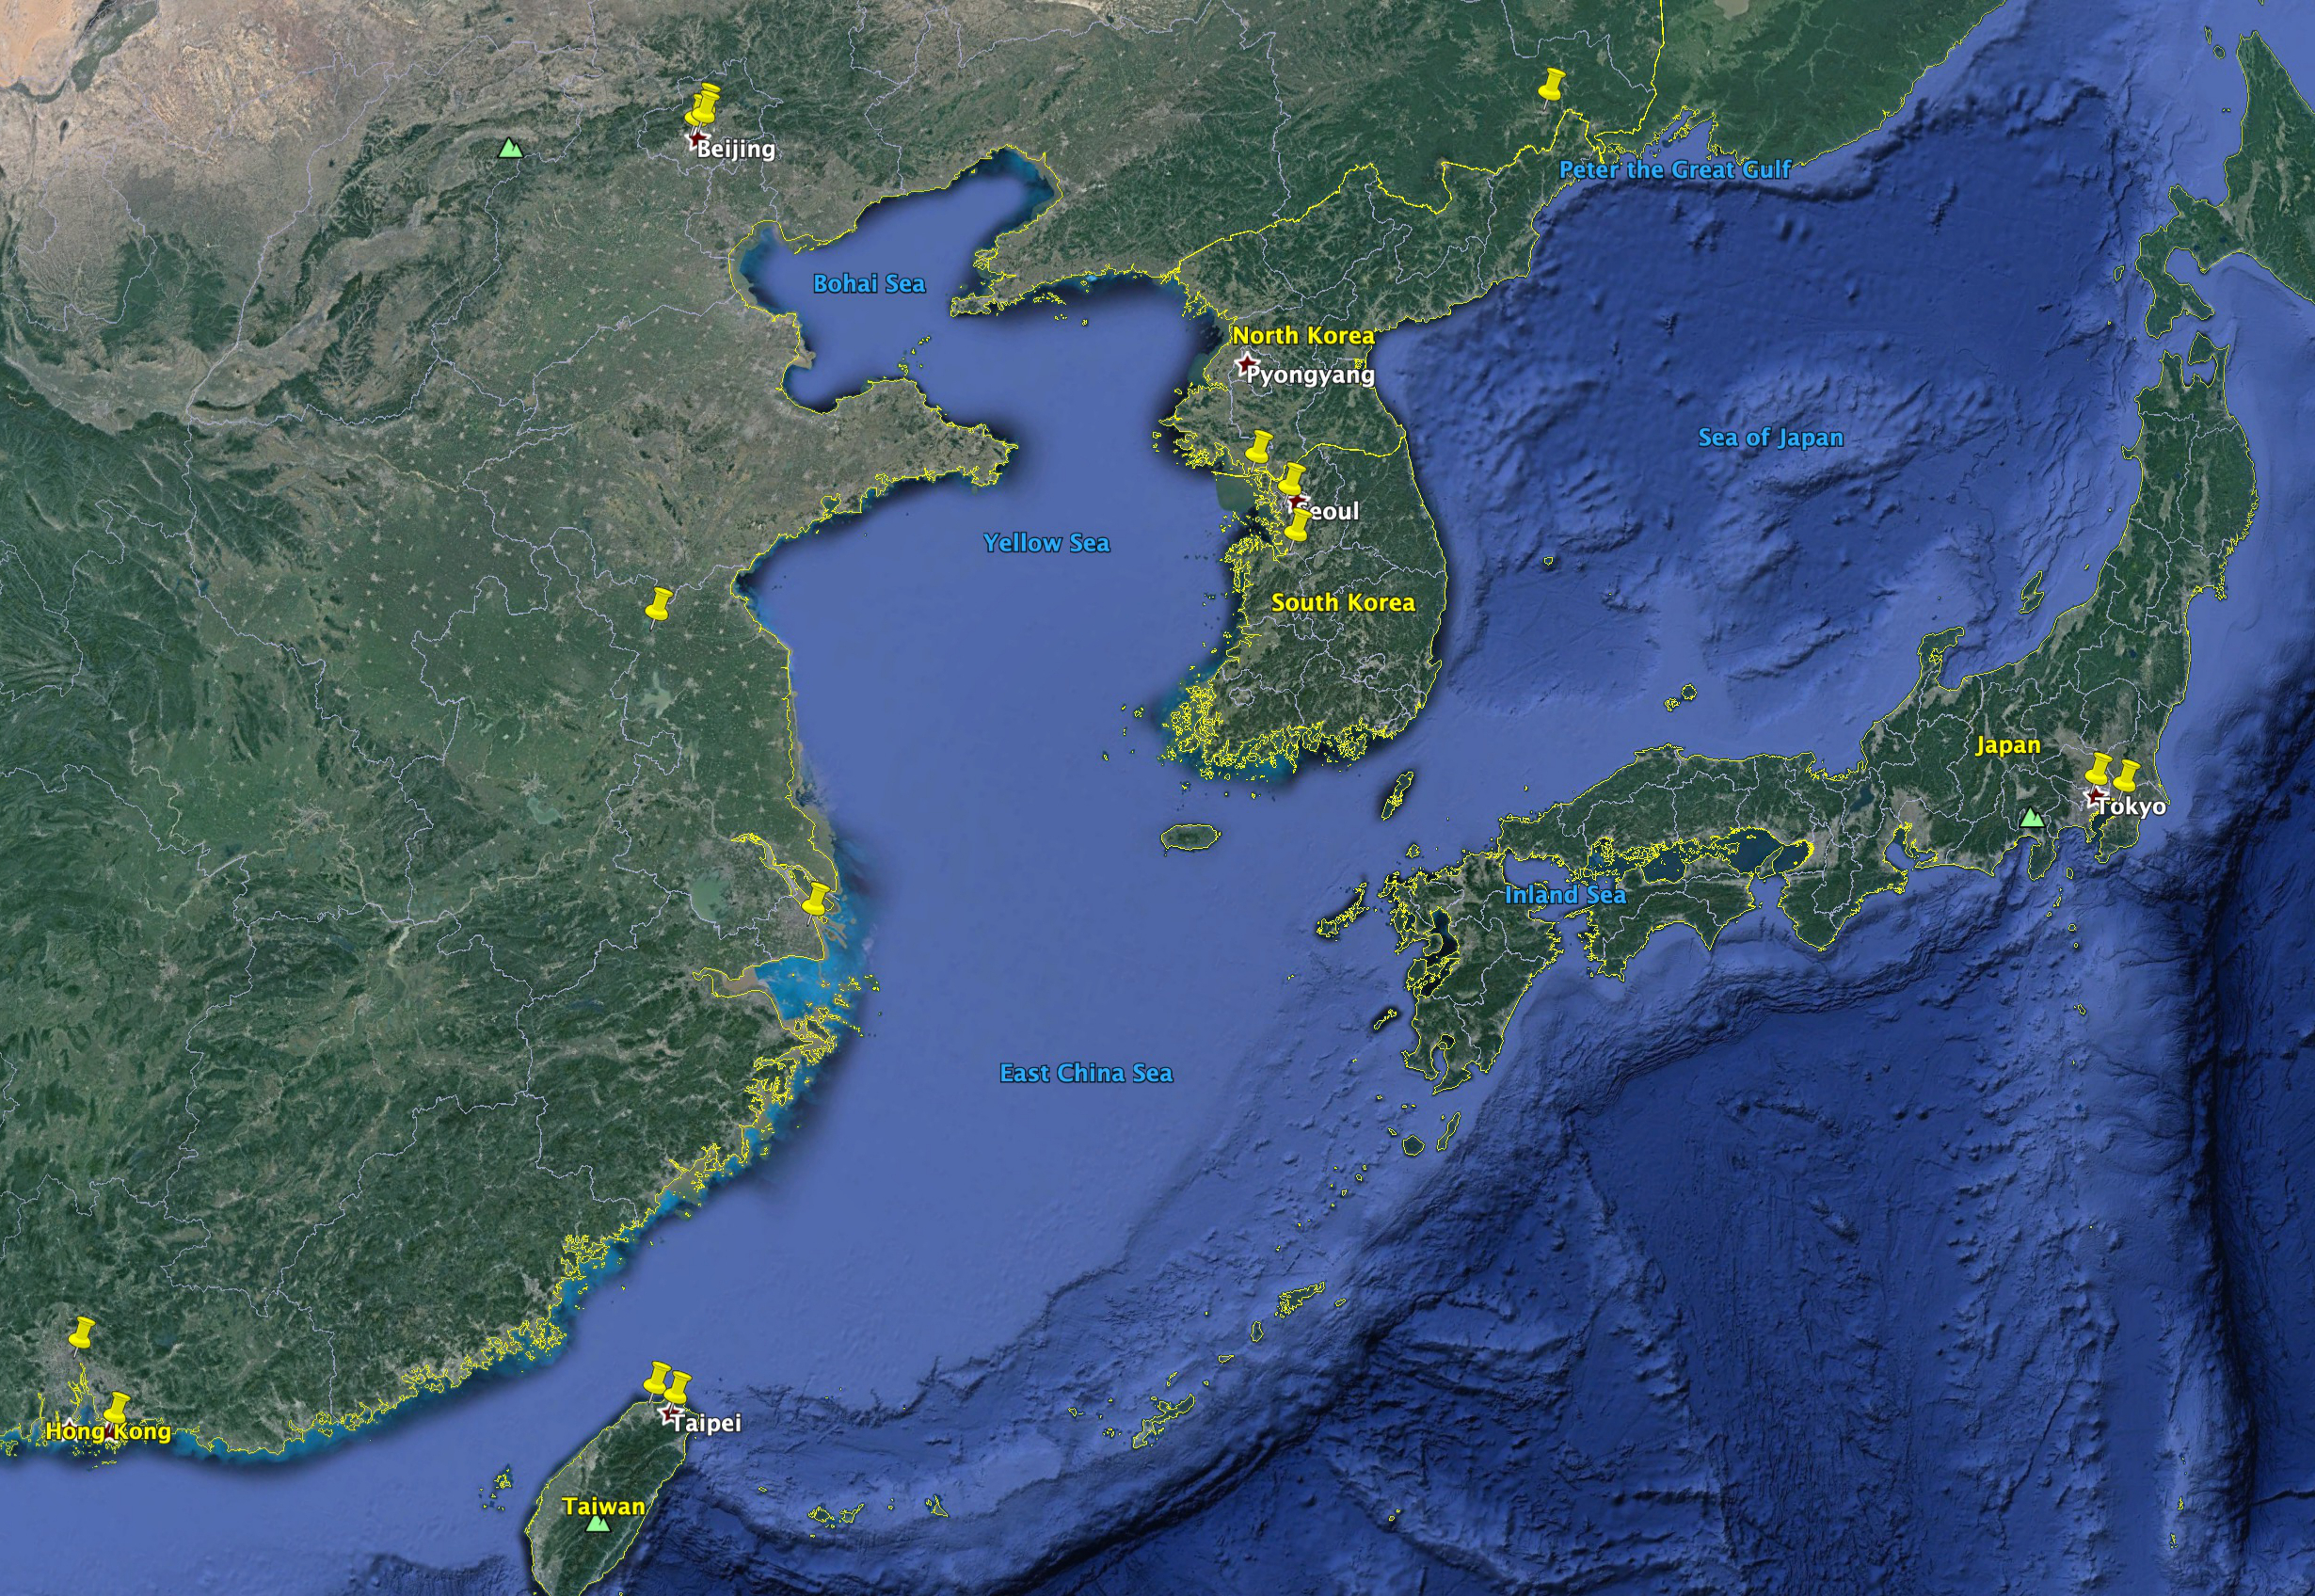
\includegraphics[width=\linewidth]{figures/lokahi_deploy_7.jpg}
	\caption{Lokahi Sensors: East Asia}
	\label{fig:lokahi_deploy_7}
\end{figure}

Here we can observe Lokahi sensors that have been deployed to China, Taiwan, Russia, South Korea, and Japan.

\section{Validate data collected by Laha deployment}\label{sec:validate-data-collected-by-laha-deployment}
Data from both experimental deployments were validated against ground truth data as described in Section~\ref{subsec:anticipated-contributions}. In the OPQ deployment, ground truth is provided by UH meters installed at the main of each building. In the Lokahi deployment, ground truth was provided by high-end calibrated microphones.

Results of data validation are provided in Section~\ref{sec:ground-truth-analysis}.

\subsection{Validate data collected by OPQ deployment}\label{subsec:validate-data-collected-by-opq-deployment}

Ground truth for the UH Manoa microgrid deployment is provided by UH system installed power meters. These meters were installed at the main of most buildings and can provide ground truth for voltage, frequency, and THD Trends, as well as provide a maximum bounds of these features enabling me to determine if the incidents we see in OPQ would have been seen by the UH meters.

The UH meters provide data Trends for voltage, frequency, and THD in rolled-up one minute windows. Each window provides descriptive statistics for the feature it is measuring including minimum, maximum, average, and standard deviation of the feature values during the one minute window. By using the minimum and maximum values, I was able to provide upper and lower bounds for whether or not the PQ incidents we observed were valid or not.

As an example, if an Incident is created by Mauka with a voltage sag down to 110V, then I would expect the nearest ground truth meter to also have a minimum voltage value near 110V for the same time window. If the minimum value from the UH meter does not show a voltage drop, then we know that Mauka identified a false positive.

I have written a separate service for OPQ called the ``ground-truth-daemon". The role of this daemon is to query the UH Manoa metering HTTP API once per hour and retrieve the previous hours worth of data for all ground truth meters co-located with an OPQ Box or near an OPQ Box. The descriptive statistics along with the meter metadata are stored in MongoDB so that OPQ data can be compared to the ground truth data to identify false positives and false negatives. The ground truth data model was described in Table~\ref{table:ground_truth}.

Since one of the core tenants of Laha is to throw away uninteresting data, we need to store all ground truth data in an effort to identify false negatives.

Two types of validation are performed. First, we compared Measurements and Trends collected by OPQ to Trend data collected by the UH meters. Then, we generated a report that showed the percent different between the two sets of meters. Any differences larger than 5 percent are recorded.

The second type of validation I performed was checking the bounds of Mauka generated Incidents. When a voltage Incident is generated, the sag or swell is compared against the minimum and maximum ground truth Trends. Differences larger than 5 percent were recorded. Validation for frequency and THD was performed in a similar way.

Results of validating OPQ data are provided in Section~\ref{subsec:ground-truth-analysis:-opq}.

\subsection{Validate data collected by Lokahi deployment}\label{subsec:validate-data-collected-by-lokahi-deployment}

Ground truth for Events and Incidents are provided by cross-referencing known source signals to data collected by the Lokahi network. Lokahi Events only become Incidents when they can be cross referenced with a known source signal. Because of this, all Incidents within Lokahi are trivially validated. Thus, it becomes a question of validating the Lokahi sensors' ability to characterize infrasonic signals of interest. To this end, I will examine results provided by Asmar~\cite{asmar19} which discuss the ability for the Lokahi sensors to be able to accurately quantify and characterize infrasound. These results can be found in Section~\ref{subsec:ground-truth-analysis:-lokahi}.

\section{Use Laha deployments to evaluate the main goals of the framework}\label{sec:use-laha-deployments-to-evaluate-the-main-goals-of-the-framework}
The main goals of this network are provided in Section~\ref{sec:anticipated-contributions-of-laha}. The Laha deployments for both OPQ and Lokahi were used to evaluate each of the main goals this framework claims to provide. First, that Laha is a generally useful framework representation for DSNs. Second, that Laha provides the ability to turn primitive sensor data into actionable data and insights. Third, that Laha's tiered management of sensor data provides metrics on maximum bounds for storage requirements and graceful degradation of DSN performance.

Each deployment requires different techniques for performing evaluation.

In the OPQ deployment, OPQ Boxes are deployed and co-located with industry standard, calibrated, reference sensors. Each of these sensors cost thousands to obtain and install, collect all the data all the time, and can only be connected to the power main as it enters a building. These sensors provide a means for verifying signals received or not received by OPQ, as well as confirming long term trend data. I have been provided access to these sensors and stored data via the Office of Energy Management at UH Manoa. The data is accessible via an HTTP API. The Office of Energy Management at UH Manoa has also provided the full schematics for the UH power grid. This was used as a ground truth for topology estimates and distributed signal analysis. OPQ Boxes are placed in strategic locations on the UH Manoa campus specifically in order to evaluate the distributed nature of PQ signals. For example, OPQ Boxes are placed on the same electrical lines as well as separate electrical lines to observe how PQ signals travel through an electrical grid.

In the Lokahi deployment, I had the opportunity to generate infrasound signals using a calibrated infrasound source~\cite{park2009rotary}. The source can be tuned to produce infrasound at configurable frequencies and amplitudes. The source works by attaching a variable pitch propeller to an electric motor that can be driven by a waveform generator. The source can generate signals that can be observed at large stand off distances, over tens of kilometers. Similar to the OPQ deployment, sensors within the Lokahi deployment were co-located with industry standard, calibrated, infrasound sensors. These sensors can provide a metric of signals that were correctly observed, incorrectly observed, or not observed at all by the Lokahi deployment. Further, infrasound itself is characterized quite well by various geophysical equations.

Evaluation of the main goals of this network are provided in the following sections. Results of these evaluations can be found in Section~\ref{sec:ground-truth-analysis}, Section~\ref{sec:results-of-generality-of-this-framework}, Section~\ref{sec:results-of-converting-primitie-data-into-actional-insights}, Section~\ref{sec:dsn-system-requirements}, and Section~\ref{sec:results-of-tertiary-goals}.

\subsection{Evaluation of the Generality of this Framework}\label{subsec:evaluation-of-the-generality-of-this-framework}
I claim that the Laha framework is useful and general enough to be applied to DSNs in different domains. To test this, I designed, developed, and deployed two DSNs. The first, OPQ, measures distributed PQ signals on the electrical grid. The second, Lokahi, observes infrasound signals traveling through the atmosphere.

To evaluate the generality of the Laha design, I provided metrics for whether or not each deployment is able to fulfill the goals of the given network.

I expect the PQ network, OPQ, to be able to detect and classify common PQ issues. I expect OPQ to observe voltage dips, voltages swells, frequency dips, frequency swells, transients, and high levels of THD. A count of these signals were kept and compared against industry standard PQ meters co-located with each sensor. By comparing these signals to the ground truth, we were able to tabulate a number of false positives and false negatives. In order to be considered effective, I would expect to be able to classify each of these common PQ signals, collect a set of each of the PQ signals while maintaining a low number of false positives and false negatives as compared to the industry standard sensors. In general, a negative result here would be not being able to detect PQ signals of a specific type or having a high number of false positives or false negatives.

Further, another stated goal of OPQ is to detect and classify distributed PQ incidents. That is, PQ signals that are observed by more than one sensor in situations where OPQ sensors are not co-located. First, I evaluated if OPQ is capable of detecting distributed PQ signals. I expect OPQ to at least observe one distributed signal during the test deployment, but would not be surprised to see many. By working with the Office for Energy Management at UH Manoa, I used a list of known PQ source events along with signals collected by OPQ and the industry standard sensors to provide a list of false positives and false negatives for the number of distributed PQ incidents observed by OPQ\@.

I expect the infrasound network, Lokahi, to be able to securely detect and report on infrasound incidents from a large collection of heterogeneous smartphone based infrasound sensors. This network prioritizes availability and security even in the face of network issues or no network at all. I claim that Laha is a useful framework for a DSN such as this and evaluated if Laha is able to meet the goals of this network.

To evaluate the effectiveness of Laha as implemented by Lokahi, I deployed 50 heterogeneous Lokahi smartphone sensors at predetermined distances from a calibrated infrasound source. I then used the calibrated infrasound source to generate infrasound signals of different amplitudes and frequencies. While signals are being generated, I disabled network access for the sensors to simulate real life network drop outs of sensors. I disabled the networks for time periods of 1 minute, 30 minutes, and 1 hour.

Then, for each sensor, I calculated the number of false positives and false negatives for detections of infrasound signals. In order for Laha to be a useful framework for Lokahi, Lokahi must demonstrate that not only can it detect infrasound signals at different frequencies and amplitudes, but it must also do this while maintaining a low number of false positives or false negatives.

Further, as availability is a major priority of this network, network outages must be handled without signal loss. To evaluate this goal, I measured the amount of false negatives (or missed signals) due to Laha's data management and the interplay with network outages. I would expect that if Lokahi implements it correctly, we should not see a rise in false negatives. A less great result would be an increase in false negatives.

Finally, backed by the metrics for both deployments, I provide a critical discussion on what types of DSNs Laha is well suited for and what types of DSNs Laha is not well suited for. This includes a discussion on which parts of the Laha design are useful or a detriment to a given goal of the DSN\@.

The following sections continue to discuss the evaluation strategies required to show that Laha is a generally useful representation for a DSN\@.

Results providing evidence the the generality of the Laha framework can be found in Section~\ref{sec:results-of-generality-of-this-framework}.

\subsection{Evaluation of Converting Primitive Data into Actionable Insights}\label{subsec:evaluation-of-converting-primitive-data-into-actionable-insights}
An important goal of any DSN is to convert primitive sensor data into actionable insights. This is generally accomplished by adding some kind of context associated with the data such as classifications of a signal or linking the data with other data by comparing similarities in time, space, or other physical features.

I claim that Laha's use of Actors acting on and moving data between levels in the Laha hierarchy provides a useful and generic approach to systematically adding context to data as it moves through the framework. Laha is designed with a specific number of levels where data within each level shares the same type. In each deployment, I evaluated the usefulness of each level with regards to adding context to the data.

An early approach to organizing data for contextualization is the Data Grid project\cite{chervenak2000data} which proposed two services for building higher level extractions, storage systems and metadata management. This framework provided the context on top of data needed to easily build replication services for the data, which was important since one of the major goals of this framework was data availability and policy management. Data Grid also maintains data uniformity and does not allow complex schemas. Data Grid does not provide a mechanism for discarding noisy data. Laha differs from Data Grid by providing support for complex metadata schemas, focuses on data reduction strategies, and provides more support for driving context. A more recent paper from Wu et al.\cite{wu2014data} presents the HACE framework which is a framework designed for applying context to Big Data by making integration with other data sources and performing data fusion a first class member of the framework. This paper also examines algorithms for mining of complex and dynamic data, such as those generated from sensor networks. Laha differs from HACE by using a tiered approach to manage data volume while still hopefully generating actionable insights.

In both deployments, I evaluated the number of false negatives for incident classification. Each level in the framework is responsible for not only adding context, but deciding if data should be moved upward through the levels, adding more context along the way, or discarding data because a level does not think the data is ``interesting". I kept track of the number of false negatives and which level was responsible for discarding the data with the signal. Using this approach, I evaluated the effectiveness of each level to determine which levels correctly identify signals and which levels do not correctly identify signals, thus discarding the data.

In order to be useful, I expect each level to add context to the data while maintaining a low level of false negatives.

Using these metrics, I provide a discussion on which domains a leveled approach may work well for versus which domains a leveled approach might not provide useful benefits. This discussion is provided in the results chapter (Section~\ref{subsec:discussion-of-laha-levels}).

I claim that Laha is able to provide additional context and actionable insights through a level called Phenomena. Phenomena utilize predictive analytics to provide context and actionable insights over the sensor domain. First, I evaluated if Phenomena take place in practice for both of the Laha deployments.

To evaluate Phenomena in the OPQ network, OPQ must observe a cyclical incident such as voltage swells occurring every afternoon due to solar output or an electric motor turning on at the same time every day. Once a cyclical incident is observed, OPQ must correctly create predictive Phenomena that predict the same incident happening in the future. Assuming predictive Phenomena are created, I measured the amount of false positive and false negative predictions. A positive result would show that now only is OPQ capable of making predictive Phenomena, but also that a high percentage ($>$ 50\%) of the predictions are correct.

Evaluation of predictive Phenomena in the Lokahi infrasound network followed a similar strategy. However, since I can control the infrasound source, I can run an experiment that creates cyclical and non-cyclical signals. I then tested Lokahi's ability to not only create predictive Phenomena, but also show that the predictions are accurate, that is, greater than 50\% of them are correct.

A negative result would be that if either of the networks are not able to create predictive Phenomena or a large number of false positives or false negatives (combining for $<$50\% prediction accuracy).

Adding context to classified Incidents is the act of providing a statistical likelihood of the underlying cause of the Incident. These include things like showing that a voltage sag is caused by turning on the dryer every day at 2PM or identifying an infrasound signal as a repetitive flight pattern near an airport. Context is provided by external sources to the DSN (such as users or by performing data fusion with other correlating data sets).

Evaluating contextualized Events consists of setting up experiments where I assign context for a specific set of signals and resulting Incidents. Then, testing to see if Phenomena are able to correctly apply context to Incidents when the same signals are generated again. I recorded the number of false positives and false negatives for assigning context to Incidents.

A positive result would be to see the correct context applied to incidents more than half of the time. That is, I expect context to be applied correctly to at more than 50\% of Incidents for which context has been previously defined.

I expect to see contextualization work better in DSNs where signals provide more measures for discrimination. For example, PQ networks contain many different types of classified PQ signals, however there is a small subset of causes attributed to each type of PQ signal classification.This decreases Laha's search space and in theory should make it easier to provide context.

Results for converting primitive data into actionable insights are provided in Section~\ref{sec:results-of-converting-primitie-data-into-actional-insights}.

\subsection{Evaluation of Tiered Management of Big Data}\label{subsec:eval-big-data}
The goal of tiered management of Big Data is to add a mechanism that provides a maximum bounds on storage requirements of sensor data at each level in the Laha hierarchy while simultaneously reducing sensor noise as Laha Actors move ``interesting" data upwards. This in turn should decrease the amount of false positives since forwarded data is more likely to include signals of interest and is less likely to be sensor noise.

Other approaches to Big Data management include compression\cite{tang2004compression} or storage systems where the goal is to have a distributed file system and move data close to where it is being processed, such as the Hadoop Distributed File System\cite{warrier2007much}. Other systems such as NiFi\cite{hughes2016survey} provide a nice interface for ingestion and movement of data between Big Data tools while also providing data provenance, but do not go far enough in focusing on data reduction and graceful degradation. Carney et al.\cite{carney2002monitoring} discuss how monitoring applications require management and clean up of stale sensor data.

\subsubsection{Evaluation of False Positives and False Negatives}\label{eval-fp-fn}
It is possible that Laha threw away data that did contain signals of interest. In this case, detection or classification Actors did not observe the signals because the data has been discarded leading to increased false negatives. On the other hand, by reducing false positives and increasing the signal-to-noise ratio as data moves upward, Phenomena has a better chance of optimizing triggering, detection, and classification which may in turn inform Laha to save data that would have been previously thrown away. In this way, it is possible that Laha reduces false negatives.

I evaluated the number of false positives and false negatives in detections, classifications, and Phenomena compared against industry standard reference sensors. A positive outcome for this metric would be a reduction in both false positives and false negatives compared to an approach that does not use tiered data management. A negative result would be an increase in either false positives or false negatives.

Results comparing collected data to ground truth data can be found in Section~\ref{sec:ground-truth-analysis}.

\subsubsection{Evaluation of DSN System Requirements}\label{sssec:eval_of_dsn_system_requirements}
I examined theoretical data storage requirements for any DSN that utilizes Laha as an abstract model.

Let us consider the theoretical bounds on storage requirements at each level in the Laha hierarchy. First we will consider the storage bounds when all parameters are known and then we will look at bounds using estimated parameters for each level.

Results for DSN system requirements are provided in Section~\ref{sec:dsn-system-requirements}.

\paragraph{IML Requirements}
The IML level contains instantaneous samples from a sensor. These values are generally stored in memory on the sensors. We can calculate several useful metrics for this layer.

First, we can calculate the IML size for an individual sensor $S_{SEN}$, with a sample size in bytes $S_{SAMP}$, a sample rate in Hz $SR$, and a time window in seconds $T$. This is shown in Equation~\ref{iml:SSEN}.

\begin{equation}\label{iml:SSEN}
	S_{SEN} = S_{SAMP} * SR * T
\end{equation}

Next, we can calculate the IML size for the entire network $S_{IML}$ by summing up the IML size for each individual sensor $B$ in the network. Equation~\ref{iml:DSEN} provides these calculations.

\begin{equation}\label{iml:DSEN}
	S_{IML} = \sum_{i=1}^{B_{n}} S_{SEN_{i}}
\end{equation}

We can estimate upper and lower bounds when the number of sensors recording data to the IML varies over time by examining the mean number of sensors that recorded data $\mu N_{SEN}$ over a time period in seconds $T$.

Equation~\ref{eq:iml:mu_size_iml} provides the calculations for finding the mean size of the IML with varying amounts of sensors.

\begin{equation}\label{eq:iml:mu_size_iml}
\mu S_{IML} = S_{SAMP} * SR * \mu N_{SEN} * T \pm \delta S_{IML}
\end{equation}

Equation~\ref{eq:iml:e1} and Equation~\ref{eq:iml:e2} provide the error bounds for calculating the mean IML size.

\begin{align}
	\delta N_{SEN} &= \frac{\sigma N_{SEN}}{\sqrt{T}} \label{eq:iml:e1} \\
	\delta S_{IML} &= \delta N_{SEN} * |S_{SAMP} * SR * T| \label{eq:iml:e2}
\end{align}

Each sample in this level is generally stored using built in machine types that generally take 1, 2, 4, or 8 bytes. Further, depending on the network requirements, each sample may or may not have an associated timestamp. Each timestamp generally adds between 4 and 8 bytes to each sample.

Table~\ref{table:iml_size} provides the expected size of the IML layer for the OPQ and Lokahi networks over time periods of one day, one week, and one year. These values are constant for all OPQ and Lokahi networks independent of deployment because they only rely on constant values defined by the sensors themselves.

\begin{table}[H]
	\centering
	\caption{IML Constraints per Sensor}
	\begin{tabularx}{\textwidth}{Xlllll}
		\toprule
		\textbf{Description} & \textbf{Rate} & \textbf{Size} & \textbf{Data/Day} & \textbf{Data/Week} & \textbf{Data/Year} \\
		\midrule
		OPQ Box & 12 kHz & 2 & 2.07 GB & 14.51 GB & 756.86 GB \\
		Lokahi Sensor & 80 Hz & 4 & 0.03 GB & 0.19 GB & 10.10 GB \\
		Lokahi Sensor & 800 Hz & 4 & 0.28 GB & 1.94 GB & 100.92 GB \\
		Lokahi Sensor & 8 kHz & 4 & 2.76 GB & 19.35 GB & 1009.15 GB \\
		\bottomrule
	\end{tabularx}
	\label{table:iml_size}
\end{table}

It is evident that the IML layer produces a significant amount of data, most of which is noise. Left unbounded an OPQ network with 15 Boxes can easily grow beyond 11 terabytes per year and a Lokahi network with 15 sensors at the maximum sampling rate can grow to over 15 terabytes per year!

\paragraph{AML Requirements}
Aggregate Measurements provide rolled-up feature extracted values generated from the IML layer. These often include multiple features (i.e.\ voltage, frequency, THD) and descriptive statistics of each feature (i.e.\ minimum, maximum, average, variance). It is worth noting that the theoretical bounds may differ from the actual bounds in practice due to the way the underlying storage engine persists the values. These differences will be examined in the results section.

Laha allows for multiple sub-levels within the AML. For instance, the OPQ DSN has both Measurements and Trends AMLs which summarize data at different window lengths. We need to take this into consideration when generating bounds for the AML\@.

To simplify calculating the bounds on the AML level, we make an assumption that the variance of the size of each AML value is close to 0. The actual metrics for each AML value remain constant sized while the metadata associated with each AML may differ in size. Since each AML value contains similar metadata, the variance on the size of the metadata should remain small.

Equation~\ref{eq:aml_sl} computes the size of a sub-level within the AML $S_{SL}$ by examining the size of an AML entry $S_{V}$, sub-level send rate in Hz $SR$, sensing time in seconds $T$, and a set of sensors $B$.

\begin{equation}\label{eq:aml_sl}
	S_{SL} = S_{V} * SR * T * B_{n}
\end{equation}

Equation~\ref{eq:aml} shows the size of the AML $S_{AML}$ including all sub-levels.

\begin{equation}\label{eq:aml}
	S_{AML} = \sum_{i=1}^{S_{SL_{n}}} S_{SL_{i}}
\end{equation}

Similar to what was done for the IML, we can estimate bounds assuming the number of sensors sending data is not constant. Equation~\ref{eq:aml:mu_s_sl} and Equation~\ref{eq:aml:mu_s_aml} provide the calculations for mean sub-AML level size and the mean size of the AML respectively.

\begin{align}
	\mu S_{SL} &= S_{V} * SR * T * \mu B \pm \delta S_{SL} \label{eq:aml:mu_s_sl} \\
	\mu S_{AML} &= \sum_{i=1}^{S_{\mu SL_{n}}} \mu S_{SL_{i}} \pm \delta S_{AML} \label{eq:aml:mu_s_aml}
\end{align}

Equation~\ref{eq:aml:e0}, Equation~\ref{eq:aml:e1}, and Equation~\ref{eq:aml:e2} provide the error on mean calculations for the AML\@.

\begin{align}
	\delta B &= \frac{\sigma B}{\sqrt{T}} \label{eq:aml:e0} \\
	\delta S_{SL} &= \delta B * |S_{V} * SR * T| \label{eq:aml:e1} \\
	\delta S_{AML} &= \sqrt{\sum_{i=1}^{\delta S_{SL_{n}}}} (\delta S_{SL_{i}}) ^ 2  \label{eq:aml:e2}
\end{align}

Table~\ref{table:aml_size} contains the theoretical bounds of the AML layer without any optimization for OPQ and Lokahi networks. These values provide the upper bounds per sensor for periods of one day, one week, and one year. The OPQ DSN utilizes two sub-levels (one for Measurements and one for Trends). The Lokahi network contains only one level, but each sampling rate has its own IML rate. We provide the upper bounds for each possible sampling rate that Lokahi utilizes. These values are constant for all OPQ and Lokahi networks independent of deployment because they only rely on constant values defined by the sensors themselves.

\begin{table}[H]
	\centering
	\caption{AML Constraints per Sensor}
	\begin{tabularx}{\textwidth}{Xlllll}
		\toprule
		\textbf{Description} & \textbf{Rate} & \textbf{Size} & \textbf{Data/Day} & \textbf{Data/Week} & \textbf{Data/Year} \\
		\midrule
		OPQ $AML_{Measurements}$ 	& 1 Hz 					& 145 			& 12.52 MB 	& 87.69 MB 	& 4.6 GB 	\\
		OPQ $AML_{Trends}$ 			& $\frac{1}{60}$ Hz 	& 325 			& 0.47 MB 	& 3.72 MB  	& 170.82 MB \\
		OPQ $AML_{Total}$ 			&   					&   			& 12.99 MB 	& 91.41 MB 	& 4.77 GB 	\\
		Lokahi $AML_{80Hz}$			& $\frac{1}{51.200}$ Hz	& 2546  		& 27.65 MB 	& 193.54 MB & 10.09 GB	\\
		Lokahi $AML_{800Hz}$		& $\frac{1}{40.960}$ Hz	& 2546		& 276.48 MB & 1.94 GB 	& 100.92 GB \\
		Lokahi $AML_{8000Hz}$		& $\frac{1}{32.768}$ Hz	& 2546		& 2.76 GB 	& 19.35 GB 	& 1.01 TB 	\\
		\bottomrule
	\end{tabularx}
	\label{table:aml_size}
\end{table}

Left unoptimized and taken over the course of a year for a typical OPQ or Lokahi deployment with 15 sensors, we would expect an upper bound of 71.55 GB collected from the OPQ network and 15 TB of data to be collected from the Lokahi network. Why is the AML so much larger in Lokahi as compared to OPQ? It is due to a requirement of the Lokahi network to store raw data along with its AML windows. Not only do Lokahi AML windows contained the feature extracted features of the stream, but they also contain the raw data associated with that window.

\paragraph{DL Requirements}
The detections level contains metadata and associated sampled high fidelity data that was returned from sensors for a given time window. A single detection can contain samples from multiple data streams for a single Event of interest.
The detections level contains metadata and associated sampled high fidelity data that was returned from sensors for a given time window. A single detection can contain samples from multiple data streams for a single Event of interest.

Similarly to the AML level, we assume that the metadata for each detection remains a constant or close to constant size and we focus on the raw data which dominates the storage requirements in the DL\@.

I make the assumption that the window lengths for each high-fidelity stream within a single detection are equally sized. In reality, it is possible that a sensor encounters an error and does not return data for the entire requested time window.

Calculating the bounds of this collection is further complicated by the fact that Detections are not generated at a constant rate and the window length of the detections can be highly variable. Further, the number of sensors that return data for any given detection is also variable. Therefore, I provide statistical calculations for these bounds.

First, let us examine calculating the bounds when all parameters are known for a sub-detection. A sub-detection is data returned from a single sensor within a detection. The bounds for each sub-detection is similar to the bounds for a single sensor in the IML, because this level contains the IML data plus some close to constant sized metadata providing context to the IML data.

Equation~\ref{eq:dl:ssd} computes the size of a sub-detection $S_{SD}$ using a given sensor sampling rate in Hz $SR$, the length of the detection in seconds $T$, and the size of the sub-detection metadata $S_{SDM}$.

\begin{equation}\label{eq:dl:ssd}
	S_{SD} = S_{SAMP} * SR * T + S_{SDM}
\end{equation}.

\begin{equation}\label{eq:dl:dl}
	S_{DL} = \sum_{i=0}^{S_{D_{n}}} S_{D_{i}}
\end{equation}

There is a clear upper bound on the size of the DL for a single sensor in the pathological case that the entire data set recorded by a single sensor is one long single Detection. In this pathological case, the upper bounds of the DL is equal to the upper bounds of the IML plus some constant metadata size. The pathological case is not incredibly useful, so, let us look at this from a statistical standpoint.

We can provide estimated bounds on the DL with an estimated data rate $\mu DR$ which provides the mean number of bytes generated per second within the DL\@. It should be noted that this includes the parameters for all sub-detections as well. The calculation for the mean size of the DL is given in Equation~\ref{eq:dl:mu_s_dl}.

\begin{equation}\label{eq:dl:mu_s_dl}
	\mu S_{DL} = \mu DR * T \pm \delta S_{DL}
\end{equation}

The errors for the mean size of the DL are given in Equation~\ref{eq:dl:e0} and Equation~\ref{eq:dl:e1}.

\begin{align}
	\delta DR = \frac{\sigma DR}{\sqrt{T}} \label{eq:dl:e0} \\
	\delta S_{DL} = \delta {DR} * |T| \label{eq:dl:e1}
\end{align}

Let us next compare the estimated sizes of the DL for the OPQ and Lokahi networks using statistics gathered for these networks. These values were obtained from actual data collected during deployments of the OPQ and Lokahi networks. Table~\ref{table:estimated_mu_dr} provides the parameters used for these comparisons.

\begin{table}[H]
	\centering
	\caption{Estimated $DR$}
	\begin{tabularx}{\textwidth}{lllll}
		\toprule
		\textbf{Network} & $\bm{\mu DR}$ & \textbf{Data/Day} & \textbf{Data/Week} & \textbf{Data/Year} \\
		\midrule
		OPQ & 40.69 & 3.51 MB & 24.77 MB & 1.29 GB \\
		Lokahi & 402.82 & 34.80 MB & 243.63 MB & 12.70 GB \\
		\bottomrule
	\end{tabularx}
	\label{table:estimated_mu_dr}
\end{table}

\paragraph{IL Requirements}
The Incidents Level provides added context on top of the DL in the form of signal of interest classifications. This level is structured similarly to the DL in that it contains trimmed down IML samples from one or more sensors over a varying time window and added context in the form of metadata. Due to these similarities, the bounds calculations are also quite similar.

The IL differs from the DL in that the associated IML samples in the IL are always subsets of the samples in the DL\@. The IL also differs from the DL in the fact that the IL does not have a concept of ``sub-incidents". Every Incident in the IL is associated with exactly one Event waveform.

When all parameters are known, the individual size of an Incident $S_{I}$ within the IL can be calculated over the size of each sample $S_{SAMP}$, sample rate in Hz $SR$, length of the incident $T+{I}$, and size of the associated metadata $S_{M}$ with Equation~\ref{eq:il:s_i}.

\begin{equation}\label{eq:il:s_i}
	S_{I} = S_{SAMP} * SR * T_{I} + S_{M}
\end{equation}

Then, computing the size of the entire IL can be done with a simple summation as shown in Equation~\ref{eq:il:s_il}.

\begin{equation}\label{eq:il:s_il}
	S_{IL} = \sum_{i=0}^{S_{I_{n}}} S_{I_{i}}
\end{equation}

There is a clear upper bound on the size of the IL for a single sensor in the pathological case that the entire data set recorded by a single sensor is one long single Incident. In this pathological case, the upper bounds of the IL is equal to the upper bounds of the IML plus some constant metadata size. The pathological case is not incredibly useful, so, let us look at this from a statistical standpoint.

We can provide estimated bounds on the IL assuming a mean Incident rate in bytes per second $\mu IR$ as shown in Equation~\ref{eq:il:mu_s_il}.

\begin{equation}\label{eq:il:mu_s_il}
 \mu S_{IL} = \mu IR * T \pm \delta S_{IL}
\end{equation}

Equation~\ref{eq:il:e0} and Equation~\ref{eq:il:e1} provide error bounds on the estimated size of the IL\@.

\begin{align}
	\delta IR &= \frac{\sigma IR}{\sqrt{T}} \label{eq:il:e0} \\
	\delta S_{IL} &= \delta IR * |T| \label{eq:il:e1}
\end{align}

Let us next compare the estimated sizes of the IL for the OPQ and Lokahi networks using statistics gathered for these networks. These values were obtained directly from data collected during OPQ and Lokahi deployments. Table~\ref{table:estimated_mu_ir} provides the parameters used for these comparisons.

\begin{table}[H]
	\centering
	\caption{Estimated $IR$}
	\begin{tabularx}{\textwidth}{llllll}
		\toprule
		\textbf{Network} & $\bm{\mu DR}$ & \textbf{Data/Day} & \textbf{Data/Week} & \textbf{Data/Year} \\
		\midrule
		OPQ & 184.41 & 15.93 MB & 111.53 MB & 5.82 GB \\
		Lokahi & 37.12 & 3.21 MB & 22.45 MB & 1.17 GB \\
		\bottomrule
	\end{tabularx}
	\label{table:estimated_mu_ir}
\end{table}

\paragraph{PL Requirements}
The Phenomena Level provides actionable insights and context beyond what is provided in the IL. Examples of added context include predictive analysis, Annotations, or similarity metrics between Incidents. The Phenomena level consists mainly of metadata describing the Phenomena. Different types of Phenomena require varying amounts of metadata.

Equation~\ref{eq:pl} calculates the size of the PL $S_{PL}$ by summing the size of each Phenomena $S_{P}$ that is stored.

\begin{equation}\label{eq:pl}
	S_{PL} = \sum_{i=0}^{S_{P_{n}}} S_{P_{i}}
\end{equation}

The size of the PL can be estimated by Equation~\ref{eq:est_pl} where $\mu PR$ is the mean Phenomena data rate per second and $T$ is the number of seconds that the network is up.

\begin{equation}
	\mu S_{PL} = \mu PR * T
	\label{eq:est_pl}
\end{equation}

Next, I will compare the estimated sizes of the PL for the OPQ and Lokahi networks using statistics gathered for these networks. These values were obtained directly from data collected during OPQ and Lokahi deployments. Table~\ref{table:estimated_mu_pl} provides the parameters used for these comparisons.

\begin{table}[H]
	\centering
	\caption{Estimated $PL$}
	\begin{tabularx}{\textwidth}{llllll}
		\toprule
		\textbf{Network} & $\bm{\mu DR}$ & \textbf{Data/Day} & \textbf{Data/Week} & \textbf{Data/Year} \\
		\midrule
		OPQ & 0.22 & 0.02 MB & 0.13 MB & 6.92 MB \\
		Lokahi & 0.01 & 0.86 kB & 6.05 kB & 314.50 kB \\
		\bottomrule
	\end{tabularx}
	\label{table:estimated_mu_pl}
\end{table}

Why are the Phenomena data amounts so low compared to the other levels? The main reason is that Phenomena are few and far between. Another reason is that Phenomena consist mainly of metadata and do not copy data from lower levels into it. Instead, Phenomena points to data in lower levels and adjusts the TTL values of lower levels to match that of the Phenomena.

\paragraph{Comparing Laha Requirements}

Now that we can compute the bounds for different levels within the Laha hierarchy, let us examine how the requirements compare between each level given data that resembles the OPQ and Lokahi DSNs. This data was generated using parameters gathered from OPQ and Lokahi deployments.

Analytically, when all parameters are known, the size of the entire DSN $S_{DSN}$ can be computed as shown in Equation~\ref{eq:s_dsn}.

\begin{equation}\label{eq:s_dsn}
	S_{DSN} = S_{IML} + S_{AML} + S_{DL} + S_{IL} + S_{P}
\end{equation}

Statistically speaking, the mean size and error of the entire DSN are provided by Equations~\ref{eq:dsn:mu_s_dsn} and Equation~\ref{eq:dsn:e} respectively.

\begin{align}
	\delta S_{DSN} &= \sqrt{(\delta S_{IML})^2 + (\delta S_{AML})^2 + (\delta S_{DL})^2 + (\delta S_{IL})^2 + (\delta S_{P})^2} \label{eq:dsn:e} \\
	\mu S_{DSN} &= \mu S_{IML} + \mu S_{AML} + \mu S_{DL} + \mu S_{IL} + \mu S_{P} \pm \delta S_{DSN} \label{eq:dsn:mu_s_dsn}
\end{align}

First, let us look at the size of Laha with parameters estimated from OPQ. The estimated parameters for this scenario are given in Table~\ref{table:estimated_laha_opq}.

\begin{table}[H]
	\centering
	\caption{OPQ Estimated Parameters}
	\begin{tabularx}{\textwidth}{ll}
		\toprule
		\textbf{Field} & \textbf{Mean} \\
		\midrule
		$S_{SAMP}$ & 2 \\
		$SR$ & 12000 \\
		$S_{MEASUREMENT}$ & 145 \\
		$R_{MEASUREMENT}$ & $\frac{1}{1}$ \\
		$S_{TREND}$ & 365  \\
		$R_{TREND}$ & $\frac{1}{60}$  \\
		$\mu N_{SEN}$ & 1  \\
		$\mu DR$ & 40.69  \\
		$\mu IR$ & 184.41 \\
		$\mu PR$ & 0.22 \\
		\bottomrule
	\end{tabularx}
	\label{table:estimated_laha_opq}
\end{table}

Figure~\ref{fig:plot_lala_opq} shows the estimated bounds of the entire network over the course of three years.

\begin{figure}[H]
	\centering
	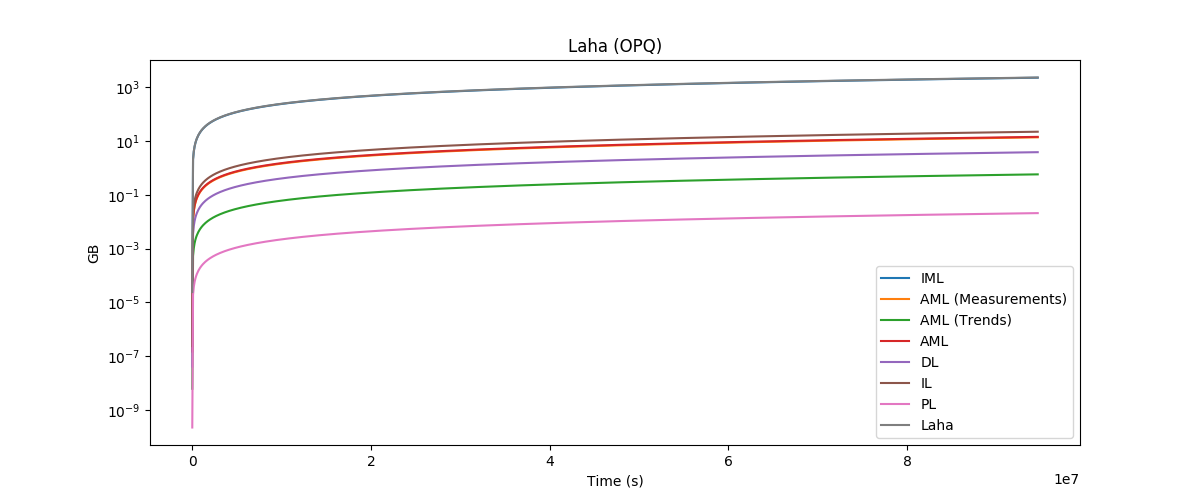
\includegraphics[width=\linewidth]{figures/plot_laha_opq.png}
	\caption{Estimated Laha (OPQ)}
	\label{fig:plot_lala_opq}
\end{figure}

We can gather that the bounds on the entire OPQ network given estimated parameters from the network are 2310 gigabytes over a period of 3 years. It is clear that the IML provides most of this data. We can also see that over time, the DL dominates all other levels except the IML\@.

By representing the data as a pie chart (Figure~\ref{fig:plot_lala_opq_pie}), we can gain a better understanding of how these levels compare at the end of a year. The first (left most) pie chart shows that the IML dominates the overall data size. This makes sense because this level represents raw samples which is always going to be the largest set of data.

By removing the IML from the results, the second pie chart (right most) shows how the other levels compare to each other. From this, we can gather that the DL is the next largest. This makes sense because the DL represents windows of samples that may or may not include Incidents, and therefore the DL should always be larger than the IL which is essentially the DL with further filtering and classification.

We also observe that the size of the AML also takes up the next largest percentage of space. This is mainly due to the fact that OPQ collects aggregate Measurements once per second. Left unbounded, this collection can become quite sizable.

\begin{figure}[H]
	\centering
	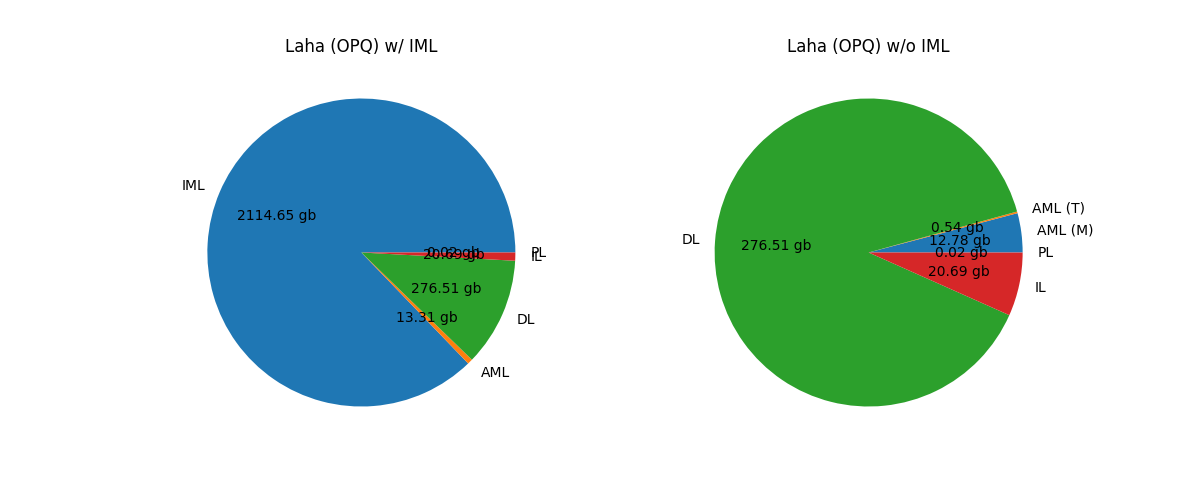
\includegraphics[width=\linewidth]{figures/plot_laha_opq_pie.png}
	\caption{Estimated Laha (OPQ)}
	\label{fig:plot_lala_opq_pie}
\end{figure}

Finally, we summarize the results in Table~\ref{table:summarized_laha_results_opq}.

\begin{table}[H]
	\centering
	\caption{Summarized Laha Results (OPQ)}
	\begin{tabularx}{\textwidth}{ll}
		\toprule
		\textbf{Laha Level} & \bm{$\mu Size$} \textbf{GB} \\
		\midrule
		IML & 2270.59 \\
		AML (Measurements) & 13.71 \\
		AML (Trends) & 0.57  \\
		AML (Total) & 14.29  \\
		DL & 3.84  \\
		IL & 22.21 \\
		PL & 0.02  \\
		Laha (Total) & 2310.97  \\
		\bottomrule
	\end{tabularx}
	\label{table:summarized_laha_results_opq}
\end{table}

Let us next perform the same evaluation, but for the Lokahi network. Table~\ref{table:estimated_laha_lokahi} provides the estimated parameters gathered from the Lokahi deployment. Since we are examining upper bounds, we will only use one of Lokahi's sampling rates (the highest 8000 Hz) in the evaluation.

\begin{table}[H]
	\centering
	\caption{Lokahi Estimated Parameters}
	\begin{tabularx}{\textwidth}{ll}
		\toprule
		\textbf{Field} & \textbf{Mean} \\
		\midrule
		$S_{SAMP}$ & 4 \\
		$SR$ & 8000 \\
		$S_{TREND}$ & 2471  \\
		$R_{TREND}$ & $\frac{1}{32.768}$  \\
		$\mu N_{SEN}$ & 1  \\
		$\mu DR$ & 402.82  \\
		$\mu IR$ & 37.11 \\
		$\mu PR$ & 0.01 \\
		\bottomrule
	\end{tabularx}
	\label{table:estimated_laha_lokahi}
\end{table}

Figure~\ref{fig:plot_lala_lokahi} shows the estimated unbounded Laha growth for Lokahi.

\begin{figure}[H]
	\centering
	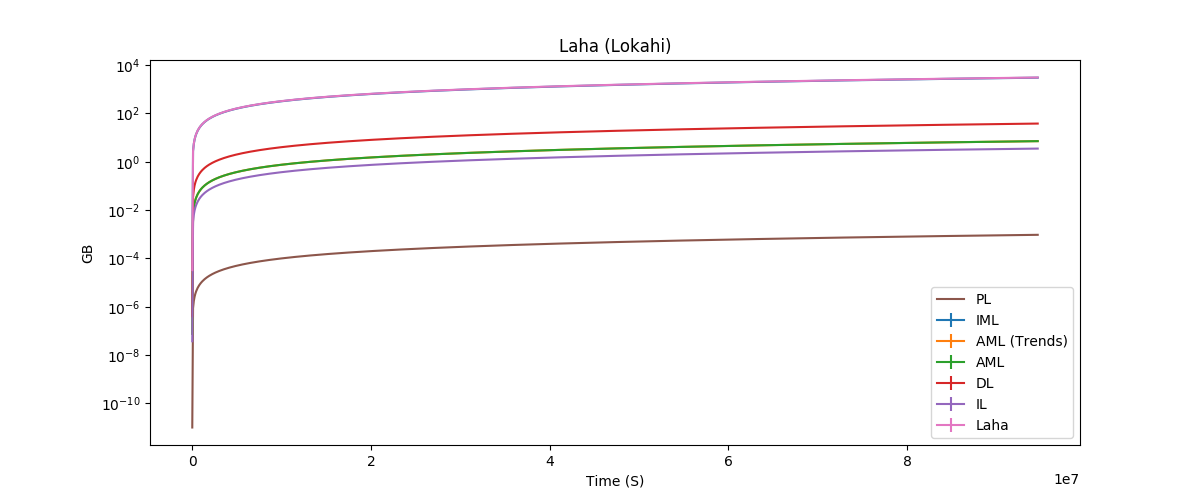
\includegraphics[width=\linewidth]{figures/plot_laha_lokahi.png}
	\caption{Estimated Laha (Lokahi)}
	\label{fig:plot_lala_lokahi}
\end{figure}

Figure~\ref{fig:plot_lala_lokahi_pie} shows the makeup of unbounded data within Laha for Lokahi.

\begin{figure}[H]
	\centering
	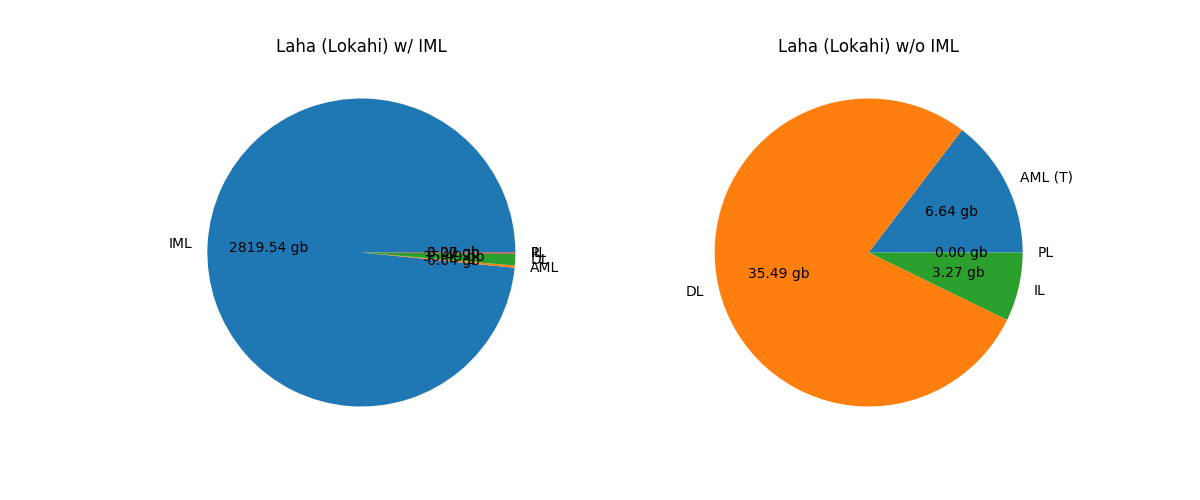
\includegraphics[width=\linewidth]{figures/plot_laha_lokahi_pie.png}
	\caption{Estimated Laha (Lokahi)}
	\label{fig:plot_lala_lokahi_pie}
\end{figure}

Finally, we summarize the results in Table~\ref{table:summarized_laha_results_lokahi}.

\begin{table}[H]
	\centering
	\caption{Summarized Laha Results (OPQ)}
	\begin{tabularx}{\textwidth}{ll}
		\toprule
		\textbf{Laha Level} & \bm{$\mu Size$} \textbf{GB} \\
		\midrule
		IML & 2819.53 \\
		AML (Total) & 6.64  \\
		DL & 35.49  \\
		IL & 3.27  \\
		PL & 0.001  \\
		Laha (Total) & 2864.95  \\
		\bottomrule
	\end{tabularx}
	\label{table:summarized_laha_results_lokahi}
\end{table}

Over the course of 3 years using estimated parameters supplied by the Lokahi network, the network is expected to grow close to 2.8 TB.

\subsubsection{Evaluation of TTL}\label{sssec:evaluation_of_ttl}
In the previous section, I examined the data requirements for Laha with the assumption that data is never discarded. In practice, this approach is unsustainable and will quickly lead to network degradation in terms of storage, memory, and processing requirements. To address this issue, Laha provides the concept of TTL (Time-to-Live) which is the amount of time that data is stored before it is garbage collected.

Each level within the Laha hierarchy provides a dynamic and configurable TTL. Data is garbage collected when it becomes older than its TTL. The TTL for data is adjusted when higher levels in the hierarchy identity something of interest. For instance, if a Detection is identified in the DL, then all data in the IML and AML that were used in the creation of the Detection are given a TTL that matches the TTL of the Detection. Similarly, if an Incident is identified in the IL, then all data in the IML, AML, and DL are given TTLs that match that of the Incident. This process continues recursively throughout all levels of the Laha hierarchy.

Table~\ref{table:ttl_summary} reviews the default TTLs provided at each level of the Laha hierarchy.

\begin{table}[H]
	\centering
	\caption{Default Laha TTL}
	\begin{tabularx}{\textwidth}{ll}
		\toprule
		\textbf{Laha Level} & \textbf{Default TTL} \\
		\midrule
		IML & 15 Minutes \\
		AML (Measurements) & 1 Day \\
		AML (Trends) & 2 Weeks \\
		DL & 1 Month \\
		IL & 1 Year \\
		PL & 2 Years \\
		\bottomrule
	\end{tabularx}
	\label{table:ttl_summary}
\end{table}

In the following sub-sections, I will look at the minimum, estimated, and maximum bounds for each level in the Laha hierarchy with TTL enabled. The minimum bounds will always be the data bounded by TTL without any data being saved by Events further up the hierarchy. The estimated bounds will be calculated using estimated parameters that quantify the amount of data in each level that is preserved by upper levels. The maximum bounds will be discussed in terms of pathological cases where all data is preserved and no data is discarded. The maximum bounds for all levels is equivalent to the bound of those levels without TTL optimization.

\paragraph{Simulating Laha}

I decided to simulate Laha using parameters gathered from the OPQ and Lokahi networks to gain insights into data storage requirements. These simulations provide estimated bounds of data on each level of the Laha hierarchy. The simulation runs at a granularity of a second and simulates the IML (raw samples), AML (Measurements and Trends), DL (Events), IL (Incidents), and PL Phenomena. The simulation maintains an in-memory database of simulated data that is sorted by TTL. Items are discarded from the database when their TTL expires. Higher levels save data from the lower levels at a similar rate as observed in the OPQ and Lokahi networks.

The following is a description of how the simulation works for the OPQ network. The simulator for the Lokahi network works similarly, but with a different estimated parameter set.

At each time step:
\begin{enumerate}
	\item 12000 samples are produced with a TTL of 15 minutes
	\item 1 Measurement is produced with a TTL of 24 hours, 1 month, 1 year, or 2 years depending on $P_{ORPHAN}(measurement)$, $P_{EVENT}(measurement)$, $P_{INCIDENT}(measurement)$, $P_{PHENOMENA}(measurement)$
	\item 1 Trend is produced if the time step if divisible by 60 with a TTL of 2 weeks, 1 month, 1 year, or 2 years depending on $P_{ORPHAN}(trend)$, $P_{EVENT}(trend)$, $P_{INCIDENT}(trend)$, $P_{PHENOMENA}(trend)$
	\item 1 Event is produced if $P_{EVENT\_STEP}$ with a TTL of 1 month, 1 year, or 2 years depending on $P_{ORPHAN}(event)$, $P_{INCIDENT}(event)$, $P_{PHENOMENA}(event)$
	\item 1 Incident is produced if $P_{INCIDENT\_STEP}$ with a TTL of 1 year or 2 years depending on $P_{ORPHAN}(incident)$, $P_{PHENOMENA}(incident)$
	\item 1 Phenomena is produced if $P_{PHENOMENA\_STEP}$ with a TTL of 2 years
	\item Garbage collection is performed if the time step is divisible by 600 ticks (10 minutes)
	\item Total items and size for each level are written to file every $N$ time steps
\end{enumerate}

Where $P_{ORPHAN}(data)$ is the probability that the referenced data does not belong to a higher level, $P_{EVENT}(data)$ is the probability that the referenced data was saved by an Detection (Event), $P_{INCIDENT}(data)$ is the probability that the referenced data was saved by an Incident, $P_{PHENOMENA}(data)$ is the probability that the referenced data was saved by a Phenomena, $P_{EVENT\_STEP}$ is the probability that an Event will be produced for any given time step, $P_{INCIDENT\_STEP}$ is the probability that an Incident will be produced for a given time step, and $P_{PHENOMENA\_STEP}$ is the probability that a Phenomena will be produced for a given time step.

Table~\ref{table:sim_params} provides the estimated parameters used to run the OPQ and Lokahi simulations.

\begin{table}[H]
	\centering
	\caption{Simulation Parameters}
	\begin{tabularx}{\textwidth}{Xll}
		\toprule
		\textbf{Parameter} & \textbf{OPQ} & \textbf{Lokahi} \\
		\midrule
		Sample Rate Hz & 12000 & 80, 800, 8000 \\
		Sample Size Bytes & 2 & 4 \\
		Measurement Rate & $\frac{1}{1}$ & N/A \\
		Measurement Size Bytes & 145 & N/A \\
		Trend Rate & $\frac{1}{1}$ & $\frac{1}{51.2}$, $\frac{1}{40.96}$, $\frac{1}{32.768}$ \\
		Trend Size Bytes & 365 & 2471 \\
		\% Data in Events & 0.16 & 6.26 \\
		\% Detections in Incidents & 55.78 & N/A \\
		Mean Event Len Seconds & 13.79 & 2010 \\
		Mean Incident Len Seconds & 0.53 & 3389 \\
		Mean Event Size Bytes & 330893 & 12923754 \\
		Mean Incident Size Bytes & 12647 & 46169741 \\
		Event DR/second & 40.66 &  0.000031 \\
		Incident DR/second & 184.41 &  0.0000008 \\
		Phenomena DR/second & 0.22 & 0.01 \\
		Simulation Tick Granularity & 1 second & 1 second \\
		Simulation Ticks & seconds/3 years, seconds/3 years, \\
		Simulation GC Interval & seconds/10 minutes, seconds/10 minutes \\
		Simulation Write Data Ticks & seconds/hour, seconds/hour \\
		\bottomrule
	\end{tabularx}
	\label{table:sim_params}
\end{table}

The full statistics can be found in the appendix in Section~\ref{appendix:simulation_parameters}.

\paragraph{Evaluation of IML with TTL}
The IML (Instantaneous Measurements Level) stores raw samples from the DSN. Traditionally, this is the largest and most noisy data set produced by the DSN and thus has a very short TTL (which is often limited by the amount of on-board sensor memory). I showed in the previous section that without TTL, this level grows very rapidly. The IML is unique in that it is the only level that does not grow beyond its TTL. Instead, when Detections, Incidents, or Phenomena are identified, data is coped from the IML into either the DL, IL, or PL. This simplifies calculating the bounds of this level.

Calculating lower bounds of the IML for a network can be accomplished by simply bounding its growth by its TTL\@. By substituting $T$ in Equation~\ref{iml:SSEN} and Equation~\ref{eq:iml:mu_size_iml} with the the number of seconds in the IML TTL (15 minutes).

Figure~\ref{fig:sim_iml_opq} shows the simulated IML data growth for a single sensor from the OPQ network over the period of one day. We can observe that the IML converges to 25 MB after 15 minutes. The spikes once the data converges is the delta added by a garbage collector that only runs once every 10 minutes.

\begin{figure}[H]
	\centering
	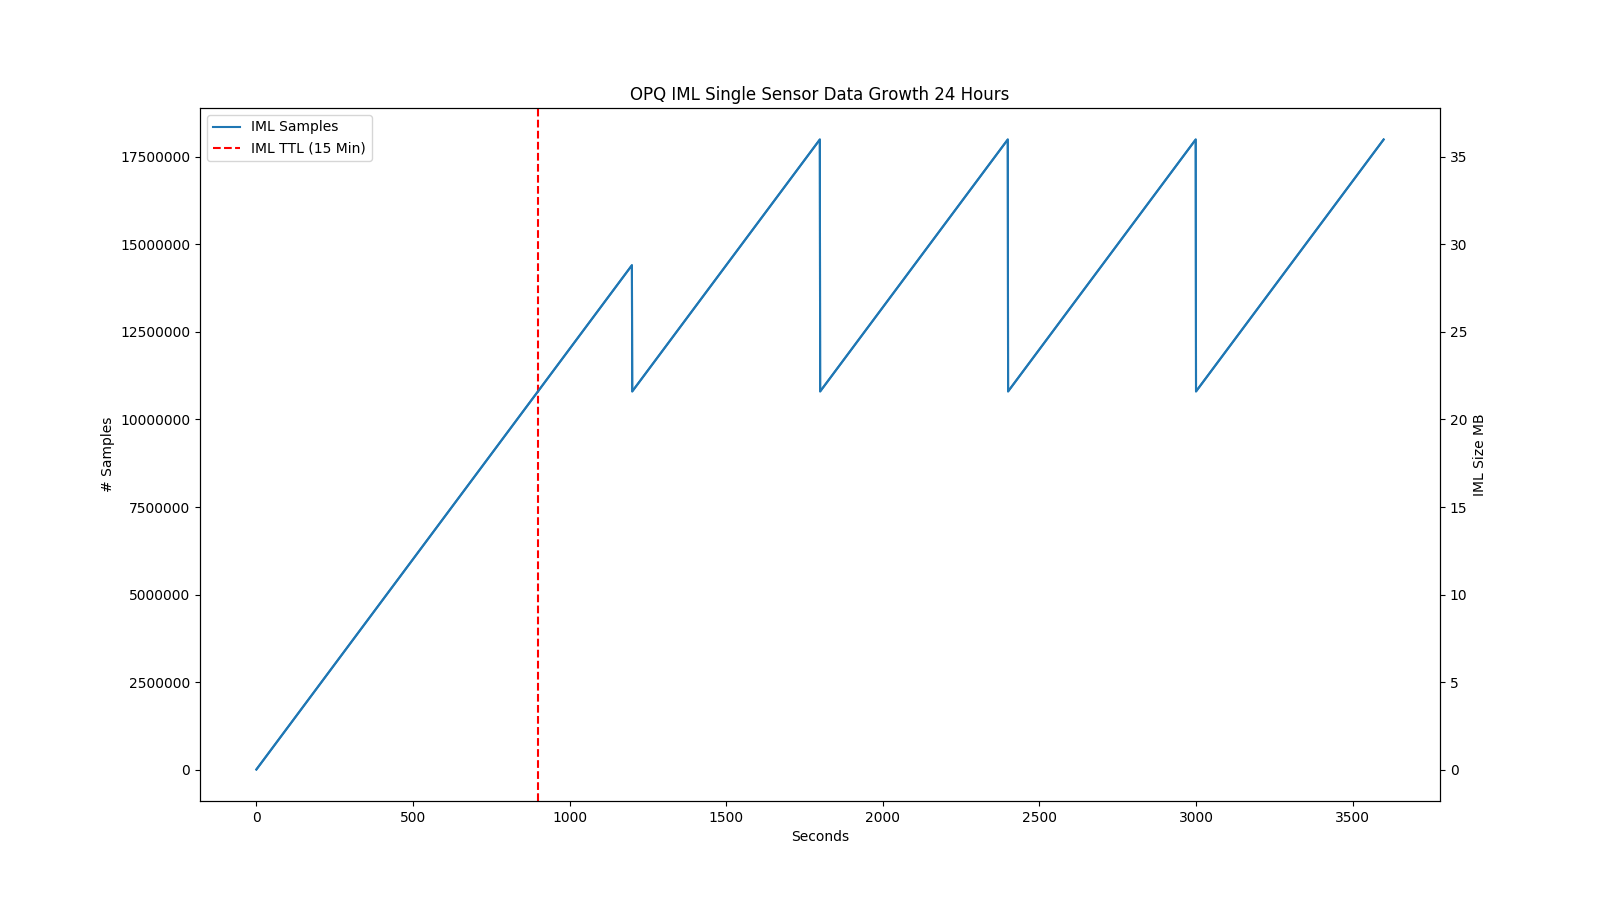
\includegraphics[width=\linewidth]{figures/sim_iml_opq.png}
	\caption{Simulated IML for OPQ}
	\label{fig:sim_iml_opq}
\end{figure}

Figure~\ref{fig:sim_iml_lokahi} shows the simulated IML data growth for a single sensor from the Lokahi network over the period of one day. Sensors within the Lokahi network have the ability to operate at different sampling rates (80 Hz, 800 Hz, or 8000 Hz) which affects the size of the IML as well as the size of every level above the IML. The simulated run of Lokahi shows the IML size differences between the different sampling rates. For one sensor, the IML converges towards 0.5 MB, 3.5 MB, and 33 MB for each sampling rate after 15 minutes.

\begin{figure}[H]
	\centering
	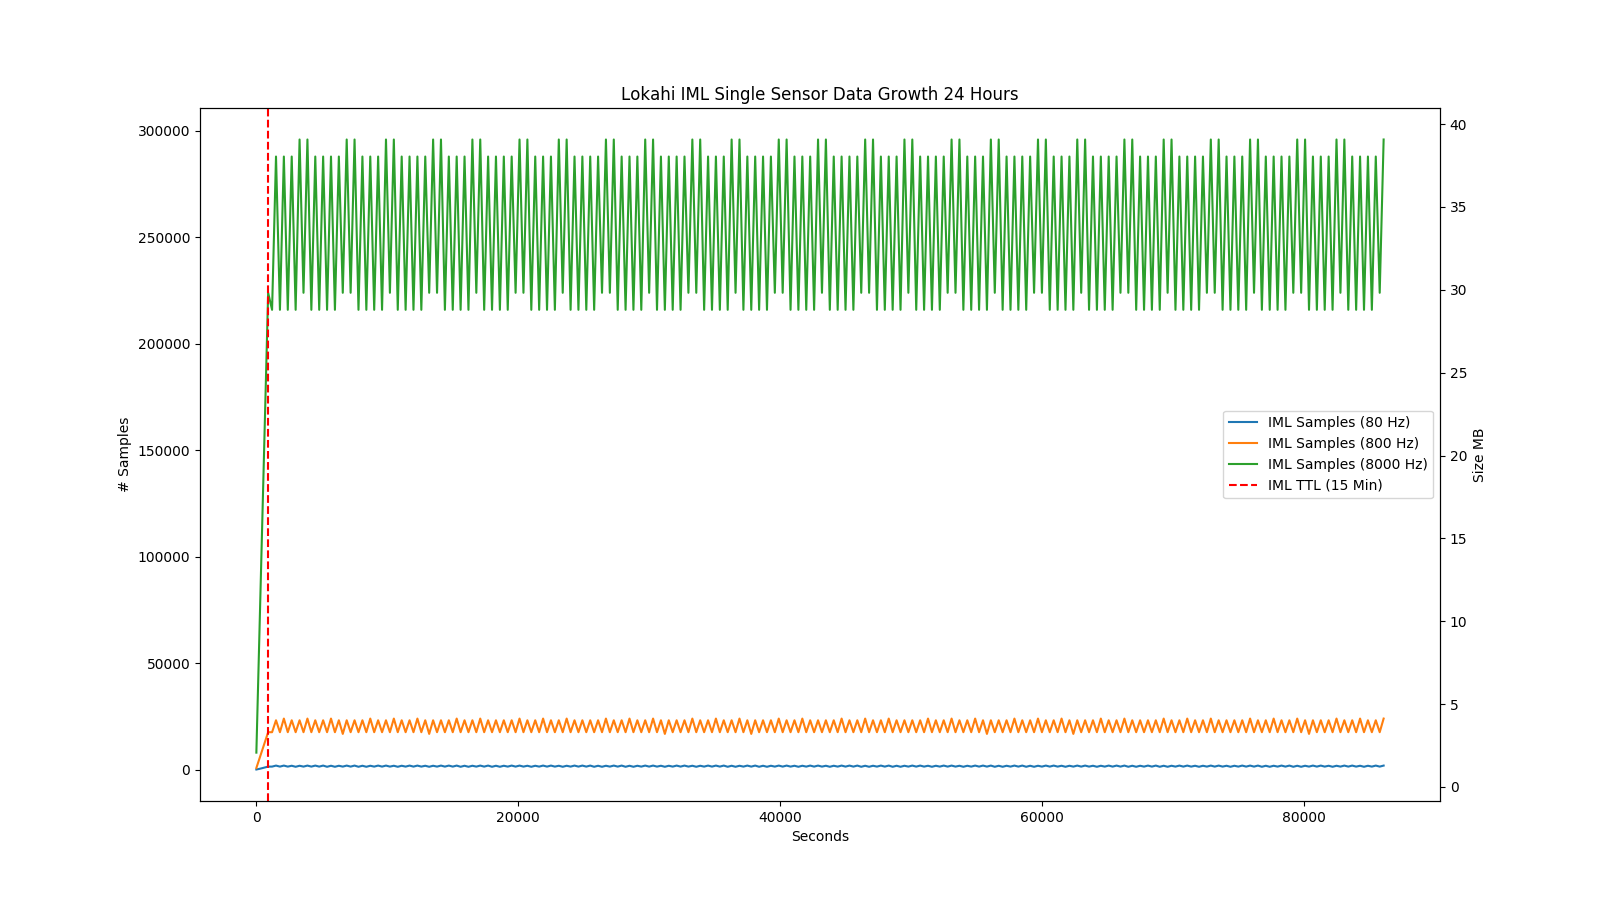
\includegraphics[width=\linewidth]{figures/sim_iml_lokahi.png}
	\caption{Simulated IML for Lokahi}
	\label{fig:sim_iml_lokahi}
\end{figure}

\paragraph{Evaluation of AML with TTL}
The AML (Aggregate Measurement Level) collects windowed features estimated from the IML data. The OPQ network provides two AMLs, Measurements which are rolled into one second windows and Trends which are rolled into one minute windows. The Lokahi network provides a single AML (Trends) with windows that vary depending on the sensor sample rate.

Table~\ref{table:ttls_aml} displays default AML TTL values for the OPQ and Lokahi networks.

\begin{table}[H]
	\centering
	\caption{Default AML TTLs}
	\begin{tabularx}{\textwidth}{Xl}
		\toprule
		\textbf{Network} & \textbf{TTL} \\
		\midrule
		OPQ (Measurements) & 1 Day \\
        OPQ (Trends) & 2 Weeks \\
        Lokahi & 2 Weeks \\
		\bottomrule
	\end{tabularx}
	\label{table:ttls_aml}
\end{table}

The minimum bounds of the AML with TTL can be found by using Equation~\ref{eq:aml:mu_s_sl} and Equation~\ref{eq:aml:mu_s_aml} and substituting $T$ for the AML TTL\@.

Next, I examine the estimated bounds of the AML by looking at the estimated amount of AML data that is saved by higher levels in the hierarchy.

Calculation of the estimated bounds can be found by Equation~\ref{eq:s_aml_ttl_full}.

\begin{equation}\label{eq:s_aml_ttl_full}
	\mu S_{AML\_TLL} = \mu S_{AML} + \mu DL_{AML} + \mu IL_{AML} + \mu PL_{AML}
\end{equation}

Where $\mu S_{AML}$ is calculated from Equation~\ref{eq:aml:mu_s_aml} and $T$ is substituted with the appropriate TTL for a given AML and $\mu DL_{AML}$ is the estimated amount of AML data saved by the DL, $\mu IL_{AML}$ is the estimated amount of AML data saved by the IL, and $\mu PL_{AML}$ is the estimated amount of AML data saved by the PL\@.

Unlike IML data which is copied when a Detection, Incident, or Phenomena is created, AML data simply has its TTL modified to match the TTL of either the Detection, Incident, or Phenomena being created. This is true of all other upper levels as well. What this means analytically is that AML data will live for as long as the highest level that that AML data reached within the Laha hierarchy. For instance, if a Detection is observed, the AML data will first receive the same TTL as the Detection. However, if an Incident is later generated from that Detection, then the AML data will receive TTLs equal to the TTL of the Incident. This must be taken into account so that AML data is not included multiple times in the calculations.

Since the estimated amount of AML data saved at each level is difficult to calculate directly, we provide the results from simulating the AML for OPQ and Lokahi.

I had to create a long simulation to observe how data saved by Detections, Incidents, and Phenomena converge over the course of the largest TTL (2 years). OPQ utilized two different types of AML data, Measurements and Trends. Each of these AML sub-types have their own TTL (1 day and 2 weeks respectively) and their own size. This was taken into consideration for the simulation and we can calculate the AML over both sub-types.

Further, the simulation tracks the amount of data at each level that is ``saved" by a higher level. If data is not ``saved" by a higher level then it retains its default TTL and I call it ``orphaned data". If data is saved by a higher lever, it gains the TTL of the highest level it is saved in and I refer to the data as ``highest\_level data". For example, ``Orphaned Measurements" refers to Measurements that have not been saved by a higher level and ``Incident Measurements" refer to Measurements that have been saved by an Incident. I will continue to use these terms to discuss the TTL bounds for the rest of the TTL evaluation.

Figure~\ref{fig:sim_aml_opq} shows the size of the AML as simulated for the OPQ network over the course of three years. This figure shows the AML bounds for both Measurements and Trends separately and shows the bounds of the entire AML in the bottom panel. The figure shows how Measurements and Trends grow until they hit the TTL they were given. A single simulated device on the OPQ network converges to near 17 MB for Measurements and 7 MB for Trends giving a total estimated bounds of near 25 MB\@.

\begin{figure}[H]
	\centering
	\includegraphics[width=\linewidth]{figures/sim_aml_opq.png}
	\caption{Simulated AML for OPQ}
	\label{fig:sim_aml_opq}
\end{figure}

Figure~\ref{fig:sim_aml_lokahi} shows the size of the AML as simulated for the Lokahi network over the course of three years. The Lokahi network does not have Measurements and only provides for a single AML sub-type, Trends. The figure shows the AML size for each available Lokahi sampling rate. The simulated AML for the Lokahi network converges to between 100 MB and 220 MB for a single sensor.

\begin{figure}[H]
	\centering
	\includegraphics[width=\linewidth]{figures/sim_aml_lokahi.png}
	\caption{Simulated AML for Lokahi}
	\label{fig:sim_aml_lokahi}
\end{figure}

It should be noted that the size difference between sampling rates is not dependent on the number of samples. In fact, the size of each Trend remains close to constant independent of the sampling rate. Rather, Trends within Lokahi are produced at different rates depending on the sampling rate. The Trend rates were chosen to support a power of 2 number of samples for efficient post processing. Table~\ref{table:lokahi_aml_rate} shows the AML Trend rates for Lokahi.

\begin{table}[H]
	\centering
	\caption{Lokahi AML Rate}
	\begin{tabularx}{\textwidth}{Xl}
		\toprule
		\textbf{Sensor Sampling Rate Hz} & \textbf{Sensor Trend Rate Hz} \\
		\midrule
		80 & $\frac{1}{51.2}$ \\
		800 & $\frac{1}{40.96}$ \\
		8000 & $\frac{1}{32.768}$ \\
		\bottomrule
	\end{tabularx}
	\label{table:lokahi_aml_rate}
\end{table}

\paragraph{Evaluation of DL with TTL}

The DL (Detections Level) contains metadata and windows of raw samples that may or may not contain signals of interest. Detections are generated when a Triggering algorithm notices deviations from nominal within the feature extracted data streams. The term ``Event" can also be used for describing a Detection. The default TTL given to Detections is one month.

The lower bounds of the DL can be found by bounding the level by its TTL and assuming that no Detections are saved by Incidents or Phenomena. This can be accomplished by substituting $T$ in Equation~\ref{eq:dl:mu_s_dl} with the Detection's TTL (1 month).

The estimated bounds can be found with Equation~\ref{eq:s_dl_ttl_full} where $\mu S_{DL}$ can be found by Equation~\ref{eq:dl:mu_s_dl}, $\mu IL_{DL}$ is the size of the DL saved by the IL, and $\mu PL_{DL}$ is the size of the DL saved by the PL\@.

\begin{equation}\label{eq:s_dl_ttl_full}
	\mu S_{DL\_TLL} = \mu S_{DL} + \mu IL_{DL} + \mu PL_{DL}
\end{equation}

Figure~\ref{fig:sim_dl_opq} shows the simulated DL for OPQ over the course of 3 years. In OPQ Detections can be orphaned or they can be saved by Incidents. The amount of Orphaned Detections converged to near 60 MB while the bulk of Detection data is due to Detections being saved by Incidents (a whopping ~700 MB of data) bringing the total DL bounds to near 800 MB\@.

\begin{figure}[H]
	\centering
	\includegraphics[width=\linewidth]{figures/sim_dl_opq.png}
	\caption{Simulated DL for OPQ}
	\label{fig:sim_dl_opq}
\end{figure}

Figure~\ref{fig:sim_dl_lokahi} shows the simulated DL for Lokahi over the course of 3 years. In Lokahi, Detections are not saved by Incidents, but rather the creation of an Incident replaces the Detection that the Incident came from. The consequence of this is that Detections only live for as long as their TTL and are never assigned a TTL of an Incident.

\begin{figure}[H]
	\centering
	\includegraphics[width=\linewidth]{figures/sim_dl_lokahi.png}
	\caption{Simulated DL for Lokahi}
	\label{fig:sim_dl_lokahi}
\end{figure}

What does affect the size of the DL in Lokahi is the sampling rate. Even if a similar number of Events are generated, higher sampling rates here will take up more space since the samples are copied into the Events.

\paragraph{Evaluation of IL with TTL}

The IL (Incident Level) contains metadata and windows of raw samples over classified signals of interest. Incidents are created when classification algorithms find signals of interest in Detection windows. The default TTL of the IL is one year.

The minimum bounds of the IL occur when IL data is strictly bounded by its TTL. This can be found by substituting $T$ in Equation~\ref{eq:il:mu_s_il} with the IL TTL (1 year).

The estimated bounds can be found with Equation~\ref{eq:s_il_ttl_full} where $\mu S_{IL}$ can be found by Equation~\ref{eq:il:mu_s_il} and $\mu PL_{IL}$ is the mean amount of IL data saved by the PL\@.

\begin{equation}\label{eq:s_il_ttl_full}
	\mu S_{IL\_TLL} = \mu S_{IL}  + \mu PL_{IL}
\end{equation}

Figure~\ref{fig:sim_il_opq} shows the simulated IL for the OPQ network over the course of 3 years. The IL converges after 1 year to near 5800 MB for a single simulated OPQ sensor.

\begin{figure}[H]
	\centering
	\includegraphics[width=\linewidth]{figures/sim_il_opq.png}
	\caption{Simulated IL for OPQ}
	\label{fig:sim_il_opq}
\end{figure}

Figure~\ref{fig:sim_il_lokahi} shows the simulated IL for the Lokahi network over the course of 3 years. Similar to the DL, the IL is affected by sensor sampling rate. The figure shows that the IL within the simulated Lokahi network converges to near 20 MB at 80 Hz, 200 MB at 800 Hz, and 2000 MB at 8000 Hz. The amount of incidents remains stable between sample rates, but the amount of data differs.

\begin{figure}[H]
	\centering
	\includegraphics[width=\linewidth]{figures/sim_il_lokahi.png}
	\caption{Simulated IL for Lokahi}
	\label{fig:sim_il_lokahi}
\end{figure}

\paragraph{Evaluation of PL with TTL}

The PL (Phenomena Level) contains metadata which provides actionable insights and context on top of Incidents. Phenomena are generated when patterns (such as periodicity) are observed in lower levels of the Laha hierarchy. The default TTL for Phenomena is 2 years.

The minimum bounds on the PL can be found by bounding the PL by its TTL (2 years).

Figure~\ref{fig:sim_pl_opq} shows the simulated growth of the PL for the OPQ network over the course of 3 years.

\begin{figure}[H]
	\centering
	\includegraphics[width=\linewidth]{figures/sim_pl_opq.png}
	\caption{Simulated PL for OPQ}
	\label{fig:sim_pl_opq}
\end{figure}

Figure~\ref{fig:sim_pl_lokahi} shows the simulated growth of the PL for the Lokahi network over the course of 3 years for a single sensor.

\begin{figure}[H]
	\centering
	\includegraphics[width=\linewidth]{figures/sim_pl_lokahi.png}
	\caption{Simulated PL for Lokahi}
	\label{fig:sim_pl_lokahi}
\end{figure}

We can observe that the size of the PL within Lokahi is similar between sampling rates. This is due to the fact that Phenomena within Lokahi are not affected by sampling rate.

\paragraph{Evaluation of Laha with TTL}

The Laha hierarchy contains the levels IML, AML, DL, IL, and PL as discussed in the previous sections. This section evaluates the bounds on the entirety of Laha by looking at all the levels in summation.

Interestingly enough, the minimum bounds of Laha can be found by summing the minimum bounds of the IML and AML. IML and AML values are always produced, but if no Events, Incidents, or Phenomena are identified, data will never be saved from IML or AML\@.

Figure~\ref{fig:sim_laha_opq} shows the simulated Laha bounds for OPQ over the course of 3 years. The figure shows that Laha for OPQ converges to near 6.5 GB per device after 1 year.

\begin{figure}[H]
	\centering
	\includegraphics[width=\linewidth]{figures/sim_laha_opq.png}
	\caption{Simulated Laha for OPQ}
	\label{fig:sim_laha_opq}
\end{figure}

Figure~\ref{fig:sim_laha_lokahi} shows the simulated Laha bounds for OPQ over the course of 3 years. The figure shows that Laha for Lokahi converges to near 250 MB at 80 Hz, 1000 MB at 800 Hz, and 8 GB at 8000 Hz per device after 1 year.

\begin{figure}[H]
	\centering
	\includegraphics[width=\linewidth]{figures/sim_laha_lokahi.png}
	\caption{Simulated Laha for Lokahi}
	\label{fig:sim_laha_lokahi}
\end{figure}

\paragraph{Comparing Laha with and without TTL}

Let us first examine OPQ\@.

Table~\ref{table:opq_laha_comparison} shows three features. The total number of data ran through the simulation at each level, the total number of data within Laha utilizing TTL, and the delta. As can be observed (and hopefully expected), we see large estimated data savings when utilizing TTL versus not utilizing TTL\@.

\begin{table}[H]
	\centering
	\caption{OPQ Laha Comparison}
	\begin{tabularx}{\textwidth}{Xlll}
		\toprule
		\textbf{Laha Level} & \textbf{Without TTL (MB)} & \textbf{With TTL (MB)} & \textbf{Delta (MB/\%)} \\
		\midrule
		IML & 2239488 & 35 & 2239453/-99.99 \\
		AML & 14097 & 25 & 14072/-99.82\\
		DL & 3931 & 750 & 3181/-80.92 \\
		IL & 17208 & 5700 & 11508/-66.87 \\
		PL & 1.38 & 0.80 MB & 0.58/-53.51 \\
		Total & 2274724 & 6510 & 2268214/-99.71 \\
		\bottomrule
	\end{tabularx}
	\label{table:opq_laha_comparison}
\end{table}

The OPQ simulation showed that of all of the Measurements and Trends, about 90.70\% of them were orphaned, 6.33\% were saved by Events, 2.97\% of them were saved by Incidents, and 0.19\% where saved by Phenomena. Of the Events, about 67.98\% were orphaned, about 31.98\% were saved by Incidents and close to 0.04\% were saved by Phenomena. Of the Incidents, about 99.9\% were orphaned while about 0.1\% were saved by Phenomena.

Let us next examine Lokahi with and without TTL. Table~\ref{table:lokahi_laha_comparison} shows three features. The total number of data ran through the simulation at each level, the total number of data within Laha utilizing TTL, and the delta. It should be noted that this example only looks at Lokahi's highest sampling rate of 8000 Hz.

\begin{table}[H]
	\centering
	\caption{Lokahi Laha Comparison}
	\begin{tabularx}{\textwidth}{Xlll}
		\toprule
		\textbf{Laha Level} & \textbf{Without TTL} & \textbf{With TTL} & \textbf{Delta (MB/\%)} \\
		\midrule
		IML & 90484 & 35 & 90449/-99.96 \\
		AML & 6987 & 220 & 6767/-96.85 \\
		DL & 180160 & 5000 & 175160/-97.22 \\
		IL & 9326 & 3000 & 6362/-67.95 \\
		PL & 0.94 & 0.20 & 0.74/-78.72  \\
		Total & 286957 & 8255 & 278702/-97.12 \\
		\bottomrule
	\end{tabularx}
	\label{table:lokahi_laha_comparison}
\end{table}

The Lokahi simulation showed that of all the Trends, about 93.21\% of them were orphaned, 6.27\% of them were saved by an Event, and about 0.26\% of them were saved by an Incident and Phenomena.

In this section, we evaluated the data storage requirements with and without TTL. We showed significant data savings when using TTL as compared to when TTL was not used. Parameters for these evaluations were found both by the physical properties of the sensors as well as the rate at which data is moved between Laha levels.

\section{Evaluation of Tertiary Goals}\label{sec:evaluation-of-tertiary-goals}
In order to achieve the main goals of this framework, I claim that either all or a subset of the following tertiary goals must be fulfilled as discussed in Section~\ref{subsec:tertiary-goals-and-claims}: optimization of triggering, detection, classification, sensor energy usage, bandwidth, predictive analytics, and the ability to derive models of the underlying sensing field topology.

To evaluate these tertiary goals, I selected and implemented DSN optimization techniques from current literature. I then compared and contrasted the usefulness of different techniques and discuss how each of these techniques perform in the different sensor domains.

Finally, I discuss how each of these tertiary goals make progress towards overall goals of this sensor network. Results of these evaluations are provided in Section~\ref{sec:results-of-tertiary-goals}.

\subsection{Evaluation of Adaptive Optimizations for Triggering}\label{subsec:evaluation-of-adaptive-optimizations-for-triggering}
Triggering is the act of observing a feature extracted data stream for interesting features and triggering sensors to provide raw data for a requested time window for higher level analysis. Adaptively optimizing triggering is a way to tune triggering algorithms and parameters with the aim of decreasing false positives and false negatives. In this context, a false positive is triggering on a data stream that does not contain a signal of interest and a false negative is not triggering on a data stream that does contain a signal of interest.

Adaptive triggering is only useful in networks that utilize triggering. Specifically, this technique can not be applied to DSNs that take a collect everything all the time approach.

Triggering can also have significant impacts on overall sensor power requirements and DSN bandwidth requirements. Many of the optimizing triggering algorithms present in the literature exist to minimize sensor energy requirements and bandwidth requirements. This is addressed in great detail in the literature review by Anastasi et al~\cite{anastasi_energy_2009}. This is accomplished by reducing communications between sensor nodes and the sink. It is argued in~\cite{pottie2000wireless} that the cost of transmitting a single bit of information from a sensor cost approximately the same as running 1000 operations on that sensor now. However, there is some contention on this topic as~\cite{alippi_adaptive_2010} argues that in some modern sensors computational requirements can equal or eclipse those of  sensor communication.

Even if a DSN utilizes triggering, it is not clear that adaptive triggering even takes place. The first question I evaluated is, does adaptive optimization of triggering take place at all given the domain of the DSN? That is, does the nature of the underlying sensor field contribute to optimization of triggering? I compared if and how optimizations take place in the two reference networks for the domains of PQ and infrasound.

In order to evaluate triggering efficiency within our Laha deployments, Laha only adaptively modifies triggering for half of the devices in the OPQ deployment. In the Lokahi deployment, I  ran the same experiment twice. The first run did not optimize triggering and the second run did optimize triggering.

Once the experiments were run, I first determined if optimization of triggering has occurred, and if it did, compared the number of false negatives and false positives against the runs that did not use optimized triggering or where optimization did not occur.

In the results chapter (Chapter~\ref{ch:results}), I will show that a side effect of Laha's optimized triggering is reduced bandwidth and sensor energy requirements. To this end, I calculated metrics for total data sent and received at the sink node of each network for each device in the network. A positive result would show decreased bandwidth usage for devices that utilize optimized triggering. A negative result would show similar or more bandwidth usage for devices that utilize optimized triggering.

Results will further show that another benefit of Laha's optimized triggering is reduced sensor energy requirements. The evaluation for this metric occurred with the Lokahi network where sensors can be dependent on batteries. I ran two experiments. For each experiment, all sensors were charged to battery level of 100\%. In the first experiment, I did not utilize optimized triggering. In the second experiment I did utilize optimized triggering. In both experiments, I measured the final battery level after the experiment and also measure how quickly the battery depletes for each sensor. This is possible because data in the Lokahi network contains timestamped entries with battery levels.

Results of adaptive optimizations for triggering can be found in Section~\ref{subsec:results-of-adaptive-optimizations-for-triggering}.

\subsection{Evaluation of Adaptive Optimizations for Detection and Classifications}\label{subsec:evaluation-of-adaptive-optimizations-for-detection-and-classifications}
Detections occur when triggering observes something ``interesting" in the feature extracted data stream. A Detection is a contiguous window of raw sensor data that was requested by triggering that may or may not contain signals of interest. Optimizing detections involves optimized the window sizes to increase the signal-to-noise ratio of the window. Fine grained features are then computed by Detection Actors and moved to the Incidents Level where classification of signals takes place. Optimizing Detections involves trimming detection windows to increase signal-to-noise. Optimizing of classifications for Incidents involves tuning parameter sets for the underlying classification algorithms.

Predictive and Locality Phenomena as well as topology optimizations were used to provide optimizations to the Detections and Incidents levels.

Evaluation of adaptive optimizations for detection and classification within the Laha network were conducted differently for each Laha deployment.

In the Lokahi deployment, I controlled the production of infrasound signals using the available infrasound source. I ran two experiments, where the amplitudes and frequencies of the signals are the same and the locations of the devices remain invariant. In the first experiment, Laha did not use optimized detection or classification provided by Phenomena. In the second experiment, Laha did use optimized detection and classification techniques provided by Phenomena.

With known frequencies and amplitudes of the infrasound signals, I can compare the rate of detections and classifications between the optimized and unoptimized experimental runs. I expect to see a greater number of and more accurate detections and classifications from the optimized experiment.

In the OPQ deployment, I compared the same metrics as the Lokahi deployment, but instead of controlling the source signal, I co-located OPQ Boxes with industry standard meters. In each pair of co-located OPQ Boxes, one was analyzed using Phenomena optimized detection and classification algorithms and the other was analyzed using unoptimized detection and classification algorithms.

I collected and evaluated the number of false positives and false negatives for Incidents generated with optimization and without optimization. A positive outcome would include a decrease in either false positives, false negatives, or both. A negative result would be an increase in either or both false positives or false negatives.

I also calculated the signal-to-noise ratio in Detections to determine if optimization of detections is working. A positive outcome is an increase in the signal-to-noise ration and a negative outcome would be similar or a decrease in signal-to-noise ratio.

Results of adaptive optimizations for detection are provided in Section~\ref{subsec:results-of-adaptive-optimizations-for-detection-and-classification}.

\subsection{Evaluation of Model of Underlying Sensor Field Topology}\label{subsec:evaluation-of-model-of-underlying-sensor-field-topology}
Laha should be able to build a model of the underlying sensing field topology. This is not the topology of the physical layout of the sensors (this is generally already known a priori or by collecting location information), but rather the topology by which signals travel. For example, in a PQ network the topology is the physical power grid and switches that PQ signals travel through. In an infrasound network, the topology is the atmosphere through which sound waves travel. Laha aims to build a statistical model of the distances between sensors according to the topology of the sensing field by observing recurrent incidents over time. This can perhaps shed some light on understanding the topology of a sensing field without knowing anything about it before hand.

Much of the literature on topology management is written to decrease sensor energy requirements by exploiting the density of sensors within a sensing field topology. For example, the ASCENT\cite{cerpa2004ascent} framework provides adaptive self configuring sensors that exploit topology denseness to decrease sensor energy usage. Several other frameworks have been designed with the same goal of reducing energy usage by exploiting topology\cite{schurgers2002stem,schurgers2002topology}.

To evaluate the model of the sensing field topology, I took two different approaches for each Laha deployment. In both deployment, the sensing field topology is known beforehand to provide a ground truth. I then compared Laha's computed signal distance between sensors to the actual signal distance between sensors as provided by the ground truths.

In the Lokahi deployment, sensors were strategically placed at different distances from an infrasound source. Some sensors were close to each other geographically, but separated by terrain that infrasound signals could not easily travel through. By moving the infrasound source, I can expect to see infrasound signals arriving or not arriving at the sensors depending on the source and direction of the signal along with the physical features of the land. By performing multiple experiments, I provided a model of the physical environment topology that Laha has built. I compared Laha's model to the known topology and provide a statistical error analysis.

In the OPQ deployment, sensors were strategically placed on electrical lines to observe how distributed PQ signals move through a power grid. In this deployment, Laha built a topology model that does not show physical geographic distance between sensors, but instead built a model of the electrical distance between sensors. This data was evaluated by comparing the electrical distances found by the Laha model to the actual UH power grid as referenced by the schematic provided by the Office of Energy Management at UH Manoa. A statistical error analysis of the differences between electrical distances between the model and the schematic is provided as an evaluation metric.

A positive outcome would be to show that there is high correlation between the Laha signal distances and the ground truth distances. A negative outcome would show low correlation.

Assuming high correlation and a statistical model of the sensing field, I evaluated if Laha is able to use this information to optimize triggering, classification, or predictive analytics. In order to evaluate this, I collected the number of false positives and false negatives at all levels in the Laha hierarchy while optimizing from topology and without optimizing from topology. I expect to see less false positives and less false negatives when utilizing topology optimizations. A negative result would be a larger number of false positives or false negatives.

I expect to only see results in networks where signals travel fast enough to create a statistical difference between arrival times at the various sensors. In sensing fields where signals travel slowly and uniformly (i.e.\ a temperature collection DSN), it may be more difficult or impossible to actually determine the sensing field topology.

Results of the underlying sensing field topology are provided in Section~\ref{subsec:results-of-model-of-underlying-sensor-field-topology}.

\chapter{Results}\label{ch:results}

\section{Results of Validating Data Collected by Deployments}\label{sec:ground-truth-analysis}

Ground truth analysis compares data collected by the OPQ and Lokahi networks to data that is assumed to be correct. The collected data is compared to the ground truth data in order to determine how similar it is to the ``correct" data. The requirement to perform ground truth analysis was provided in Section~\ref{subsec:anticipated-contributions}. The analysis performed in the next sections utilized the evaluation method from Section~\ref{sec:validate-data-collected-by-laha-deployment} in an attempt to provide evidence that the Lokahi and OPQ networks collect data that is as close to correct as possible and provides discussions on when and why this data does not always exactly match the ground truth data.

\subsection{Ground Truth Analysis: OPQ}\label{subsec:ground-truth-analysis:-opq}

The UHM Office of Energy Management provided our team with access to data collected by high quality power meters installed at the mains of selected campus buildings. This data set provides the basis of the ground truth data that I compare to OPQ using the evaluation outlined in Section~\ref{subsec:validate-data-collected-by-opq-deployment}.

Ground truth data was scraped from an UHM internal server over the duration of the OPQ deployment. I collected ground truth data containing 15 features for each of the ground truth meters that are co-located with an OPQ Box. The ground truth data is mostly complete, however, there are a few missing features for some meters.

The provided ground truth data is similar to OPQ Trends in that it provides rolled up summary statistics for features over a window of 60 seconds. The included statistics include the actual, minimum, maximum, average, and standard deviation of the features measured. Unfortunately, the ground truth data does not provide a count of how many Measurements were rolled into their one minute window. Because of this, I do not know the window sized used when computing things such as frequency or THD.

I collected the following available features for ground truth data: ``Frequency", ``Average Voltage THD", ``VAB", ``VAN", ``VBC", ``VBN", ``VCA", ``VCN", ``Voltage CN THD", ``Voltage AN THD", ``Voltage BN THD", and ``Voltage CN THD".

The frequency and THD Measurements are in units that are similar to what OPQ collects (frequency @ 60Hz and \% THD), but the voltage values are in RMS at 420V and 240V where OPQ collects RMS at 120V. This means that the voltage values can not be compared directly and that we either need to scale the voltage values or use straight thresholds for determining Events and Incidents. Further, the ground truth values for voltage are provided for each of the three voltage phases whereas OPQ Boxes compute RMS voltage from a combination of three phases. This needs to be considered before comparing ground truth voltage to OPQ voltage Measurements.

Although the frequency and THD ground truth Measurements are scaled the same as OPQ observations, it is not clear what size of computation window the ground truth sensors utilize to make these calculations. I expect to see slight differences between what Mauka observed and what the UHM meters observed due to these differences.

To complicate things, we do not have a UHM meter co-located with every OPQ Box and several of our Boxes are co-located with multiple UHM meters making the determination of which combination of Box and Meter to compare not straight forward.

Finally, it should be noted that due to OPQ's default TTL values, Measurements are only stored for a day and Trends are only stored for two weeks. This means that we can not compare the ground truth Trends directly (unless they were saved by an Event, Incident, or Phenomena) for more than a period of 2 weeks. This only affects comparing ground truth data to OPQ Measurements and Trends and should not affect the comparison of Events and Incidents.

Table~\ref{table:gt} provides a mapping from OPQ Boxes to co-located UHM meters.

\begin{table}[H]
    \centering
    \caption{OPQ Boxes Co-Located with UHM Ground Truth Sensors}
    \begin{tabularx}{\textwidth}{lX}
        \toprule
        \textbf{OPQ Boxes} & \textbf{UHM Ground Truth Sensors} \\
        \midrule
        1000, 1002 (POST) & POST\_MAIN\_1 \\
         & POST\_MAIN\_2 \\
        1001 (Hamilton) & HAMILTON\_LIB\_PH\_III\_CH\_1\_MTR \\
         & HAMILTON\_LIB\_PH\_III\_CH\_2\_MTR \\
         & HAMILTON\_LIB\_PH\_III\_CH\_3\_MTR \\
         & HAMILTON\_LIB\_PH\_III\_MAIN\_1\_MTR \\
         & HAMILTON\_LIB\_PH\_III\_MAIN\_2\_MTR \\
         & HAMILTON\_LIB\_PH\_III\_MCC\_AC1\_MTR \\
         & HAMILTON\_LIB\_PH\_III\_MCC\_AC2\_MTR \\
        1003 (Keller) & KELLER\_HALL\_MAIN\_MTR \\
        1005 (Parking Structure Ph. II) & N/A \\
        1006 (Frog I) & N/A \\
        1007 (Frog II) & N/A \\
        1008 (Mile's Office) & N/A \\
        1009 (Watanabe) & N/A \\
        1010 (Holmes) & N/A \\
        1021 (MSB) & MARINE\_SCIENCE\_MAIN\_A\_MTR \\
         & MARINE\_SCIENCE\_MAIN\_B\_MTR \\
         & MARINE\_SCIENCE\_MCC\_MTR \\
        1022 (Ag. Engineering) & AG\_ENGINEERING\_MAIN\_MTR \\
         & AG\_ENGINEERING\_MCC\_MTR \\
        1023 (Law Library) & LAW\_LIB\_MAIN\_MTR \\
        1024 (IT Building) & N/A \\
        1025 (Kennedy Theater) & KENNEDY\_THEATRE\_MAIN\_MTR \\
        \bottomrule
    \end{tabularx}
    \label{table:gt}
\end{table}

As can be observed, several OPQ Boxes do not have a co-located UHM sensor and several OPQ Boxes are co-located with multiple UHM sensors.

\subsubsection{Frequency Measurement and Trend Ground Truth Analysis}

Measurements and Trends are both computed on-board OPQ Boxes using the same algorithms. Since Trends live longer than Measurements, we will perform these comparisons using Trends only for frequency, THD, and voltage. A comparison directly to Measurements would yield similar results since Trends are computed directly from the Measurements.

Frequency Trends can be compared one-to-one with the UH ground truth meters using the ``Frequency" feature provided by ground truth sensors. In the following Figures, I compare the observed OPQ frequencies to the observed co-located UHM meter frequencies.

For each frequency comparison, I aligned the two series by minute and then subtracted two weeks of OPQ observed frequencies from the UHM observed frequencies. I then plotted the differences as a histogram and finally model a best fit of a Normal Distribution on top of the histogram. This approach is also used when comparing against voltage and THD Trends.

As an example, Figure~\ref{fig:f_hist} shows the frequency observed by OPQ Box 1000 in POST compared to the UHM POST\_MAIN\_1 meter.

\begin{figure}[H]
    \centering
    \includegraphics[width=0.75\linewidth]{figures/f_hist_1000_POST_MAIN_2.png}
    \caption{Frequency OPQ Box 1000 vs POST\_MAIN\_1}
    \label{fig:f_hist}
\end{figure}

The rest of the frequency comparisons look very similar and the results are summarized in Table~\ref{table:gt_f}.

\begin{table}[H]
    \centering
    \caption{Frequency Trend Comparisons}
    \begin{tabularx}{\textwidth}{lXll}
        \toprule
        \textbf{OPQ Box} & \textbf{UHM Ground Truth Sensor} & \boldmath{$\mu$} & \boldmath{$\sigma$} \\
        \midrule
        1000 & POST\_MAIN\_1 & -0.0018 & 0.0079 \\
        1000 & POST\_MAIN\_2 & -0.0017 & 0.0079 \\
        1001 & HAMILTON..CH\_1 & -0.0007 & 0.0074 \\
        1001 & HAMILTON..CH\_2 & -0.0010 & 0.0074 \\
        1001 & HAMILTON..CH\_3 & -0.0012 & 0.0074 \\
        1001 & HAMILTON..MAIN\_1 & -0.0013 & 0.0074 \\
        1001 & HAMILTON..MAIN\_2 & -0.0011 & 0.0074 \\
        1001 & HAMILTON..MCC\_AC2 & -0.0009 & 0.0074 \\
        1002 & POST\_MAIN\_1 & -0.0018 & 0.0069 \\
        1002 & POST\_MAIN\_2 & -0.0017 & 0.0069 \\
        1003 & KELLER\_HALL\_MAIN & -0.0006 & 0.0073 \\
        1021 & MARINE\_SCIENCE\_MAIN\_A & -0.0010 & 0.0081 \\
        1021 & MARINE\_SCIENCE\_MAIN\_B & -0.0006 & 0.0081 \\
        1021 & MARINE\_SCIENCE\_MCC & 0.0003 & 0.0081 \\
        1022 & AG\_ENGINEERING\_MAIN & -0.0020 & 0.0078 \\
        1022 & AG\_ENGINEERING\_MCC & -0.0018 & 0.0078 \\
        1023 & LAW\_LIB\_MAIN & -0.0005 & 0.0078 \\
        1025 & KENNEDY\_THEATRE\_MAIN & -0.0013 & 0.0087 \\
        \bottomrule
    \end{tabularx}
    \label{table:gt_f}
\end{table}

As can be observed, the OPQ Boxes that we have co-located with UHM ground sensors track the frequency quite accurately. In general we rarely see differences outside of 0.02 Hz and most sensors show a mean difference on the order of a mHz. These results are expected as grid stability relies heavily on the frequency. Further, frequency is generally affected at global scales rather than local scales, so we expect all UHM meters and OPQ Boxes to observe similar frequency trends across the UHM micro-grid.

\subsubsection{Voltage Ground Truth Analysis}

OPQ Boxes measure RMS voltage as a combination of three voltage phases at 120 Volts. UHM ground truth meters measure RMS voltage for each individual phase at different voltages (480, 240, and 270). Because of these differences, the voltages can not be compared directly and can only be performed for a small subset of our Boxes due to available ground truth data (those that contain voltage channels for ``AB", ``BC", and ``CA").

In order to compare OPQ Box voltages against UHM voltages, a combination of voltage values must exist within the ground truth data for each sensor with the following configurations: voltage from phase A to phase B, voltage from phase B to phase C, and voltage from phase C to phase A. If these metrics exist, then the RMS value for the ground truth can be found by Equation~\ref{eq:gt_vrms} as described by Horowitz\cite{Horowitz:2015:AE:2960712} where $V_{AB}$, $V_{BC}$, and $V_{CA}$ provide the inter-phase voltages reported by the UHM meters and $C$ is a constant dependent on the transformer configuration and the final step down voltage. $C$ was empirically found to be 3.9985 for our data sets.

\begin{equation}
    V_{RMS} = \frac{1}{\sqrt{3}C} \sqrt{V_{AB}^2 + V_{BC}^2 + V_{CA}^2}
    \label{eq:gt_vrms}
\end{equation}

As an example, Figure~\ref{fig:v_hist} provides the difference in $V_{RMS}$ between OPQ Box 1000 and the UHM POST\_MAIN\_1 meter.

\begin{figure}[H]
    \centering
    \includegraphics[width=0.75\linewidth]{figures/v_hist_1000_POST_MAIN_1.png}
    \caption{Voltage OPQ Box 1000 vs POST\_MAIN\_1}
    \label{fig:v_hist}
\end{figure}

Box 1000 averages about .9V higher than what is observed at the ground truth meter.

Some of the difference comparisons display multiple distributions which might be explained by the cycling of voltage conditioning equipment and by larger loads on the grid during day time hours. However, I do not have enough information about the UH micro-grid detailed operations to be completely certain about these claims.

For example, Figure~\ref{fig:v_hist_ii} compares Box 1001 in POST to the POST\_MAIN\_1 meter.

\begin{figure}[H]
    \centering
    \includegraphics[width=0.75\linewidth]{figures/v_hist_1002_POST_MAIN_1.png}
    \caption{Voltage OPQ Box 1002 vs POST\_MAIN\_1}
    \label{fig:v_hist_ii}
\end{figure}

The green Gaussian fit shows voltages collected during night time hours where the orange Gaussian fit shows values collected during the day time hours. It is interesting that Box 1000 and Box 1002 show such different results even though the Boxes are located on the same floor within the same building. The Boxes are however opposite each other within the building. I suspect that these Boxes are serviced by different electrical mains within the building. These claims are further supported by THD ground truth analysis in the following section which contains THD data for each electrical main.

Even more interesting is that several of our voltage comparisons show three separate Gaussian distributions. As example, Figure~\ref{fig:v_hist_iii} compares voltage values between Box 1021 and the MARINE\_SCIENCE\_MAIN\_A\_MTR.

\begin{figure}[H]
    \centering
    \includegraphics[width=0.75\linewidth]{figures/v_hist_1021_MARINE_SCIENCE_MAIN_A_MTR.png}
    \caption{Voltage OPQ Box 1021 vs MARINE\_SCIENCE\_MAIN\_A\_MTR}
    \label{fig:v_hist_iii}
\end{figure}

Here we can see that most of our values average about 1V higher than that of the ground truth with other peaks at 0.3V and 1.4V above the ground truth data.

Table~\ref{table:gt_v} summarizes the voltage comparisons.

\begin{table}[H]
    \centering
    \caption{Voltage Trend Comparisons}
    \begin{tabularx}{\textwidth}{lXll}
        \toprule
        \textbf{OPQ Box} & \textbf{UHM Ground Truth Sensor} & \boldmath{$\mu$} & \boldmath{$\sigma$} \\
        \midrule
        1000 & POST\_MAIN\_1 & -0.9040 & 0.1077 \\
        1001 & HAMILTON..CH\_1 & -2.8192 -2.1797 -1.5725 & 0.2291 0.1516 0.2321 \\
        1001 & HAMILTON..CH\_2 & -3.0246 -2.3877 -1.7756 & 0.2310 0.1514 0.2285 \\
        1001 & HAMILTON..CH\_3 & -2.6499 -2.0276 -1.4360 & 0.2426 0.1419 0.2255 \\
        1001 & HAMILTON..MAIN\_1 & -2.5372 -1.9135 -1.3196 & 0.2346 0.1396 0.2361 \\
        1001 & HAMILTON..MAIN\_2 & -2.3670 -1.7215 -1.1026 & 0.2392 0.1519 0.2132 \\
        1001 & HAMILTON..MCC\_AC1 & -2.7611 -2.0735 -1.4276 & 0.2242 0.1886 0.2092 \\
        1001 & HAMILTON..MCC\_AC2 & -2.6994 -2.0377 -1.4231 & 0.2413 0.1674 0.2115 \\
        1002 & POST\_MAIN\_1 & -2.8143 -1.7634 & 0.1113 0.1041 \\
        1021 & MARINE\_SCIENCE\_MAIN\_A & -1.4293 -1.0043 -0.3454 & 0.0849 0.1406 0.1802 \\
        1021 & MARINE\_SCIENCE\_MAIN\_B & 0.9882 1.4071 2.0456 & 0.0720 0.1312 0.2049 \\
        1021 & MARINE\_SCIENCE\_MCC & -1.6304 -1.2121 -0.5738 & 0.0887 0.1300 0.1894 \\
        1022 & AG\_ENGINEERING\_MAIN & 0.0947 & 0.1704 \\
        1022 & AG\_ENGINEERING\_MCC & 0.0482 & 0.1703 \\
        1023 & LAW\_LIB\_MAIN & 0.6286 & 0.1841 \\
        \bottomrule
    \end{tabularx}
    \label{table:gt_v}
\end{table}

The POST (1000), MSB, Ag. Engineering, and Law Library buildings provide the most accurate comparisons to ground truth with average differences between .5V and 1V.

Hamilton Library is a major outlier in that the ground truth comparisons are generally off by around 1.5 to 2.5 Volts. Hamilton Library is fed by three electrical mains each with multiple channels. Ground truth data is only collected on Hamilton Ph III. I suspect that our Box in Hamilton is serviced by one of the other phases. This claim is further supported by the THD comparison in the next section.

\subsubsection{THD Ground Truth Analysis}

Total Harmonic Distortion (THD) is collected by both OPQ Boxes and UHM ground truth sensors. The feature that was used to make THD comparisons is the AVERAGE\_VOLTAGE\_THD from the ground truth data. Similar to the frequency comparison, I subtracted the OPQ THD observations from the UHM THD observations and created histograms of the differences. I also attempted to fit the data with a Normal Distribution, but had less success than with the frequency. This is due to the fact that several of the distribution do not follow a Gaussian, but instead present two separate Gaussian distributions.

The multiple distributions appear to be related to time of day and point towards either power conditioning equipment cycling on and off or an increased electrical load causing higher amounts of THD during the day (or perhaps both). When there are multiple THD distributions, the distribution throughout the night time hours is more accurate than the distribution created during day time hours.

Figure~\ref{fig:gt_thd_i} compares THD between the Pacific Ocean Science and Technology building (POST) OPQ Boxes and POST UHM sensors.

\begin{figure}[h]
    \begin{tabular}{cc}
        \subfloat[1000 vs. POST\_MAIN\_1]{\includegraphics[width = 0.45\linewidth]{figures/thd_hist_1000_POST_MAIN_1.png}} &
        \subfloat[1000 vs. POST\_MAIN\_2]{\includegraphics[width = 0.45\linewidth]{figures/thd_hist_1000_POST_MAIN_2.png}} \\
        \subfloat[1002 vs. POST\_MAIN\_1]{\includegraphics[width = 0.45\linewidth]{figures/thd_hist_1002_POST_MAIN_1.png}} &
        \subfloat[1002 vs. POST\_MAIN\_2]{\includegraphics[width = 0.45\linewidth]{figures/thd_hist_1002_POST_MAIN_2.png}} \\
    \end{tabular}
    \caption{UHM THD vs. OPQ THD (POST)}
    \label{fig:gt_thd_i}
\end{figure}

The THD comparisons within the POST building provides several interesting features to discuss.

First, POST has two ground truth meters (POST\_MAIN\_1 and POST\_MAIN\_2) and two OPQ Boxes (1000 in the Collaborative Software Development Lab (CSDL) and 1002 in ICSpace). Both OPQ Boxes are on the third floor, roughly opposite each other in the building. As mentioned previously, I do not know exactly which electrical subsystem each OPQ Box is on when there are multiple electrical mains servicing a single building. In the case of POST, there are two electrical mains. I believe it is possible to guess which OPQ Box corresponds with which main by looking at the ground truth comparisons.

For instance, OPQ Box 1000 vs. POST\_MAIN\_2 provides a much smaller spread in THD difference (about .25\% THD) than OPQ Box 1000 vs. POST\_MAIN\_2 which has a spread of close to 1\% THD. I speculate that OPQ Box 1000 is on the same main as the POST\_MAIN\_2 meter. The opposite holds true for OPQ Box 1002. The spread for Box 1002 is smaller for POST\_MAIN\_1 (about 0.3\% THD) than it is for POST\_MAIN\_2 (about 0.6\% THD) which leads me to speculate that Box 1002 may be serviced by the same electrical main as the POST\_MAIN\_1 meter. These assumptions fit with assumptions made about the voltage comparisons in the previous sections providing credence to the idea that 1000 and 1002 are serviced by separate mains with POST.

Table~\ref{table:gt_thd} summarizes the best Gaussian fit for THD comparisons between OPQ Boxes and available ground truth data.

\begin{table}[h]
    \centering
    \caption{THD Trend Comparisons}
    \begin{tabularx}{\textwidth}{lXll}
        \toprule
        \textbf{OPQ Box} & \textbf{UHM Ground Truth Sensor} & \boldmath{$\mu$} & \boldmath{$\sigma$} \\
        \midrule
        1000 & POST\_MAIN\_1 & -0.5759 -0.1327 & 0.0556 0.0928 \\
        1000 & POST\_MAIN\_2 & 0.0123 0.1200 & 0.0270 0.0320 \\
        1001 & HAMILTON..CH\_1 & 1.4245 & 0.4121 \\
        1001 & HAMILTON..CH\_2 & 1.4327 & 0.4114 \\
        1001 & HAMILTON..CH\_3 & 1.3943 & 0.4153 \\
        1001 & HAMILTON..MAIN\_1 & 1.4314 & 0.4072 \\
        1001 & HAMILTON..MAIN\_2 & 0.9872 1.6370 & 0.1339 0.3078 \\
        1001 & HAMILTON..MCC\_AC1 & 1.4338 & 0.4132 \\
        1001 & HAMILTON..MCC\_AC2 & 1.4441 & 0.4133 \\
        1002 & POST\_MAIN\_1 & 0.0888 0.2154 & 0.0367 0.0415 \\
        1002 & POST\_MAIN\_2 & 0.3875 0.6652 & 0.0655 0.0796 \\
        1021 & MARINE\_SCIENCE\_MAIN\_A & -0.6964 & 0.1156 \\
        1021 & MARINE\_SCIENCE\_MAIN\_B & 0.3098 0.5649 & 0.0725 0.0601 \\
        1021 & MARINE\_SCIENCE\_MCC & -0.6938 & 0.1160 \\
        1022 & AG\_ENGINEERING\_MAIN & 0.5406 & 0.0421 \\
        1022 & AG\_ENGINEERING\_MCC & 0.4993 & 0.0433 \\
        \bottomrule
    \end{tabularx}
    \label{table:gt_thd}
\end{table}

All comparisons (except for those at Hamilton Library) show average differences of around .5\% THD. Similar to what was discussed in the previous section comparing voltage values, Hamilton remains the single outlier in our data set. Here, I observed upwards of 1.5\% THD difference across Hamilton based meters. This continues to lead me to believe that the OPQ Box in Hamilton is serviced by a different main that that of the HAMILTON\_PH\_III ground truth meters.

To summarize the comparison of OPQ Measurements and Trends to ground truth data, I showed that co-located OPQ Boxes and UHM ground truth meters trend quite closely together (except for at Hamilton Library) for low level metrics. Frequency is the most accurate metric, followed by THD and voltage. I would have liked to have seen smaller differences and tighter bounds on the voltage and THD comparisons, but differences of .5\% THD and .5V are still acceptable. I also wish I had a more concrete explanation for the multiple Gaussian distributions present in the THD and voltage comparisons.

\subsubsection{Mauka Event Ground Truth Analysis}

Events contain metadata and a window of raw data that may or may not contain signals of interest. Events are produced in OPQ by two components. Mauka's threshold based Event detector and Napali's statistical based Event detector. This section focuses on Mauka's threshold based Event detection methods as the Napali Event Trigger is the focus of another Ph.D. dissertation in our research group.

Events generated by Mauka do not store information about which metric was used to generate that Event (frequency, voltage, or THD). When Mauka's Event detector was implemented, this seemed reasonable as Events are not supposed to make any type of assumption about what is non-nominal about the data, only that something non-nominal was observed.

Future implementations of the Mauka Event detector should store extra metadata about which metric was used to create an Event. This metric would be useful when comparing Events generated by Mauka to ground truth data using thresholding analysis.

In order to compare Mauka Events to ground truth data, I applied similar thresholds to those used by Mauka's Event detector to the ground truth data. The thresholds that were applied are $\pm$.16\% nominal frequency, $\pm$2.5\% nominal voltage, and +3\% THD. I then normalized the ground truth data by centering each feature's thresholds at zero and then counted the number of zero crossings for each feature and threshold for that feature.

Because the ground truth data is averaged over a minute window, I bin all Events by minute windows as well and only count windows that contain Events. I then compared the number of Events found by thresholding the ground truth data to the binned Events observed by Mauka. The results are shown in Table~\ref{table:gt_events}.

\begin{table}[h]
    \centering
    \caption{Events Comparisons}
    \begin{tabularx}{\textwidth}{lXll}
        \toprule
        \textbf{OPQ Box} & \textbf{UHM Ground Truth Sensor} & \textbf{OPQ Events} & \textbf{Ground Truth Events} \\
        \midrule
        1000 & POST\_MAIN\_1 & 580 & 928 \\
        1001 & HAMILTON\_LIB..CH\_1 & 291 & 394 \\
        1001 & HAMILTON\_LIB..CH\_2 & 291 & 380 \\
        1001 & HAMILTON\_LIB..CH\_3 & 291 & 371 \\
        1001 & HAMILTON\_LIB..MAIN\_1 & 291 & 375 \\
        1001 & HAMILTON\_LIB..MAIN\_2 & 291 & 615 \\
        1001 & HAMILTON\_LIB..MCC\_AC2 & 291 & 375 \\
        1002 & POST\_MAIN\_1 & 2678 & 928 \\
        1021 & MARINE\_SCIENCE\_MAIN\_A & 3613 & 379 \\
        1021 & MARINE\_SCIENCE\_MAIN\_B & 3613 & 821 \\
        1021 & MARINE\_SCIENCE\_MCC & 3613 & 391 \\
        1022 & AG\_ENGINEERING\_MAIN & 1605 & 929 \\
        1022 & AG\_ENGINEERING\_MCC & 1605 & 1138 \\
        \bottomrule
    \end{tabularx}
    \label{table:gt_events}
\end{table}

To perform this comparison, I required all three major features used by Mauka's Event generator, frequency (``Frequency"), voltage (``VAB", ``VBC", and ``VCA"), and THD (AVERAGE\_VOLTAGE\_THD). Ground truth data with all required features only provides co-located UHM sensors for OPQ Boxes 1000, 1001, 1002, 1021, and 1022.

Boxes 1000, 1001, and 1022 provide the best comparisons to ground truth. Mauka observes about 63\% of the ground truth Events for Box 1000 and 78\% for Box 1001. Mauka observed about 30\% more Events for Box 1022 as compared to ground truth data.

Boxes 1002 and 1021 show fairly anomalous results compared to the ground truth.

One useful observation is that the main force driving Event generation within Mauka is THD Events. THD thresholds were set at 3\% for Event generation. Most ground truth data shows that ~80\% of all Events generated are likely caused by crossing the THD thresholds with close to 18\% being caused by voltage threshold crossings. Only a very small percentage of Events generated were generated by frequency threshold crossings. This means that observed differences in THD and voltage readings between OPQ Boxes and ground truth sensors explain the differences that can be observed between ground truth data and OPQ Boxes.

For example, let us examine Box 1021 as a case study which observed 3,613 Events while ground truth only observed 391 Events. Figure~\ref{fig:gt_all_msb} shows the ground truth data for the MARINE\_SCIENCE\_MCC\_MTR sensor.

\begin{figure}[H]
    \centering
    \includegraphics[width=\linewidth]{figures/gt_all_1021_MARINE_SCIENCE_MCC_MTR.png}
    \caption{Ground Truth MARINE\_SCIENCE\_MCC\_MTR}
    \label{fig:gt_all_msb}
\end{figure}

From the previous section, we saw Box 1021 observed THD that averages 0.7\% higher than what the ground truth observed. Adding the .7\% THD difference to the ground truth shown above pushes the THD just over threshold and causes Box 1021 to produce many more Events than what was observed by ground truth initially. These results are provided in Figure~\ref{fig:gt_adj_msb}.

\begin{figure}[H]
    \centering
    \includegraphics[width=\linewidth]{figures/gt_adj_1021_MARINE_SCIENCE_MCC_MTR.png}
    \caption{Ground Truth Adjusted THD MARINE\_SCIENCE\_MCC\_MTR}
    \label{fig:gt_adj_msb}
\end{figure}

Adding the average .7\% to the ground truth data increased the number of observed ground truth THD Events from 391 to 1252 bringing the total ground truth Events to 1562.

Perhaps the THD threshold is a bit too aggressive for Event generation and future work should look at relaxing this threshold a bit and observe how that affects the results.

The results for Box 1002 can also be explained using similar methodology. Figure~\ref{fig:gt_all_post_1} shows the ground truth readings at POST\_MAIN\_1.

\begin{figure}[H]
    \centering
    \includegraphics[width=\linewidth]{figures/gt_all_1002_POST_MAIN_1.png}
    \caption{Ground Truth POST\_MAIN\_1}
    \label{fig:gt_all_post_1}
\end{figure}

This time, THD is not the cause of the large difference in the comparison. Instead, it is the voltage readings. Box 1002 reads on average 1.7 Volts higher than what is reported by ground truth. Figure~\ref{fig:gt_adj_post_1} shows the ground truth data adjusted to be 1.7 Volts higher.

\begin{figure}[H]
    \centering
    \includegraphics[width=\linewidth]{figures/gt_adj_1002_POST_MAIN_1.png}
    \caption{Ground Truth Voltage Adjusted POST\_MAIN\_1}
    \label{fig:gt_adj_post_1}
\end{figure}

Here, we can observe that the voltage values are often passing the high voltage threshold. This increases the number of voltage Events from 34 to 1141 bringing the total observed ground truth Events to 2035 or 643 Events less than what OPQ Box 1002 observed.

What these results show is that the ground truth comparisons are largely affected by observed readings of THD and voltage values by OPQ Boxes. These results also show that OPQ Boxes that produce large numbers of Events are caused by readings that hover near the feature thresholds that are utilized for Event creation.

The results from Event ground truth comparison are encouraging. The results show that although we may not be reading exactly what the ground truth sensors are reading, when adjusted for differences in low level metrics, expected Mauka Events match that of the ground truth data.

The next section will compare Mauka Incidents to ground truth data.

\subsubsection{Mauka Incident Ground Truth Analysis}

The OPQ ground truth data does not contain concepts that are related to Laha Incidents. In fact, the further we get away from the metrics that the ground truth provides (rolled-up one minute summaries), the harder it is to compare to higher levels in the Mauka hierarchy.

Instead, I apply thresholding to the ground truth data to determine where Incidents should have been observed verses when they were actually observed by Mauka. To complicate the matter, the OPQ ground truth data only provides features at a granularity of one minute. Therefore, I bin each individual Incident by minute and only count the number of bins that contain Incidents, similar to what was done for Events.

Using thresholding breaks down for many of the Incident types that rely on the duration of a disturbance to apply a classification (which is almost all of them). For instance, all IEEE defined PQ classifications rely on accurate durations of anomalous signals to apply a classification. This also holds true for Incidents that utilize industry standards such as ITIC or Semi-F47. These Incident types can not be compared to the ground truth data directly since ground truth data does not provide any notion of duration and only averages values over a one minute time window which is much too large for almost all of Mauka's Incident classifications. The best I can do for comparing Incidents is attempting to ensure that the threshold bounds make sense.

Incidents were compared using one month of data from December 1 to December 30.

\paragraph{Voltage Incidents Comparison}

Voltage Incidents include voltage sags, swells and interruptions as well as Semi-F47 and ITIC classifications. All voltage Incidents rely on the duration of the Incident in order to provide an accurate classification. Duration information is not provided by ground truth data. Instead, I use thresholding to determine where OPQ Incidents might have been observed. It is important to note here that Incidents observed by the ground truth data may not meet the duration thresholds to be classified by OPQ. I attempt to motivate this point using data from Events.

Table~\ref{table:gt_v_incidents} summarizes the results for the voltage Incidents comparisons. Please note the abbreviations in the table where ``O." stands for an OPQ Box and ``U." stands for a UHM sensor.

\begin{table}[H]
    \centering
    \caption{Voltage Incidents Comparisons}
    \begin{tabularx}{\textwidth}{lXllll}
        \toprule
        \textbf{OPQ Box} & \textbf{UHM Ground Truth Sensor} & \textbf{O.Sags} & \textbf{O.Swells} & \textbf{U.Sags} & \textbf{U.Swells} \\
        \midrule
        1000 & POST\_MAIN\_1 & 0 & 0 & 2 & 108 \\
        1000 & POST\_MAIN\_2 & 0 & 0 & 2 & 346 \\
        1001 & HAMILTON\_LIB..CH\_1 & 34 & 0 & 90 & 8 \\
        1001 & HAMILTON\_LIB..CH\_2 & 34 & 0 & 104 & 2 \\
        1001 & HAMILTON\_LIB..CH\_3 & 34 & 0 & 82 & 10 \\
        1001 & HAMILTON\_LIB..MAIN\_1 & 34 & 0 & 80 & 12 \\
        1001 & HAMILTON\_LIB..MAIN\_2 & 34 & 0 & 38 & 18 \\
        1001 & HAMILTON\_LIB..MAIN\_AC1 & 34 & 0 & 90 & 12\\
        1001 & HAMILTON\_LIB..MAIN\_AC2 & 34 & 0 & 84 & 10\\
        1002 & POST\_MAIN\_1 & 2 & 0 & 2 & 108 \\
        1002 & POST\_MAIN\_2 & 2 & 0 & 2 & 346 \\
        1021 & MARINE\_SCIENCE\_MAIN\_A & 8 & 0 & 296 & 0 \\
        1021 & MARINE\_SCIENCE\_MAIN\_B & 8 & 0 & 2 & 62 \\
        1021 & MARINE\_SCIENCE\_MCC & 8 & 0 & 664 & 0 \\
        1022 & AG\_ENGINEERING\_MAIN & 8 & 0 & 48 & 10 \\
        1022 & AG\_ENGINEERING\_MCC & 8 & 0 & 52 & 10 \\
        1023 & LAW\_LIB\_MAIN & 0 & 0 & 30 & 10 \\
        \bottomrule
    \end{tabularx}
    \label{table:gt_v_incidents}
\end{table}

There are a couple of things to note here. Mauka did observe 8 voltage swells over this time period, all for Box 1008. However, we do not have ground truth data for this location and Mauka did not observe any other voltage swells with co-located ground truth sensors.

All counts for OPQ are less than the counts shown by the OPQ ground truth data. This is important because the ground truth data does not provide any metric for swell or sag duration. This means that some percentage of the ground truth sags and swells durations are less than what is required to classify the data as an Incident by OPQ Mauka.

One of the reasons Mauka likely did not classify many voltage swells is because they are much less common in general. Further, according to Power Standards Lab\cite{power_standards_lab_2017}, voltage swells tend to be much smaller in duration compared to voltage sags. This is due to the fact that voltage swells are almost always caused by an abrupt decrease in load on the grid followed by rapid stabilization. Voltage sags on the other hand are caused by an increased load on the grid and last for as long as that load continues to persist. It is likely the voltage spikes observed by the UHM sensors did not last long enough in duration to be classified as Mauka Incidents, however without more detailed ground truth data, this is only a hypothesis.

\paragraph{THD Incidents Comparison}

I compared THD observed by the UHM ground truth meters to THD observed by OPQ Boxes.

The OPQ Box computes THD over a window of six cycles. The window size that the UHM ground truth sensors utilize for THD calculations is unknown. Because the Mauka THD plugin computes THD per electrical cycle, I expect the THD generated by Mauka to be slightly higher than that of the OPQ Box Measurements or Trends which compute THD over a larger window.

This is caused by using a smaller THD computation window which has less of a chance to average out noise. On one hand, this provides THD per cycle which better exemplifies small transients in the data which would otherwise be averaged out using larger window lengths. On the other hand, measured THD will be higher due to added noise in the signal.

I empirically found that THD values calculated by Mauka add .5\% THD to the OPQ Box and UHM ground truth Measurements. This added THD is due to added noise in the THD calculation caused by using a smaller window. Ground truth data had this constant added before comparing to THD Incidents produced by Mauka. Table~\ref{table:gt_thd_incidents} summarizes the results of the THD Incidents comparison.

\begin{table}[H]
    \centering
    \caption{THD Incidents Comparisons}
    \begin{tabularx}{\textwidth}{lXllll}
        \toprule
        \textbf{OPQ Box} & \textbf{UHM Ground Truth Sensor} & \textbf{OPQ THD} & \textbf{UHM THD} \\
        \midrule
        1000 & POST\_MAIN\_1 & 3 & 0 \\
        1000 & POST\_MAIN\_2 & 3 & 0 \\
        1001 & HAMILTON\_LIB\_PH\_III\_CH\_1\_MTR & 41 & 456 \\
        1001 & HAMILTON\_LIB\_PH\_III\_CH\_2\_MTR & 41 & 464 \\
        1001 & HAMILTON\_LIB\_PH\_III\_CH\_3\_MTR & 41 & 281 \\
        1001 & HAMILTON\_LIB\_PH\_III\_MAIN\_1\_MTR & 41 & 491 \\
        1001 & HAMILTON\_LIB\_PH\_III\_MAIN\_2\_MTR & 41 & 465 \\
        1001 & HAMILTON\_LIB\_PH\_III\_MCC\_AC1\_MTR & 41 & 456 \\
        1001 & HAMILTON\_LIB\_PH\_III\_MCC\_AC2\_MTR & 41 & 443 \\
        1002 & POST\_MAIN\_1 & 3 & 0 \\
        1002 & POST\_MAIN\_2 & 3 & 0 \\
        1021 & MARINE\_SCIENCE\_MAIN\_A\_MTR & 59 & 0 \\
        1021 & MARINE\_SCIENCE\_MAIN\_B\_MTR & 59 & 481 \\
        1021 & MARINE\_SCIENCE\_MCC\_MTR & 59 & 0 \\
        1022 & AG\_ENGINEERING\_MAIN\_MTR & 21 & 111 \\
        1022 & AG\_ENGINEERING\_MCC\_MTR & 21 & 61 \\
        \bottomrule
    \end{tabularx}
    \label{table:gt_thd_incidents}
\end{table}

These results are not surprising. Similar to the voltage Incidents, we observe that OPQ Boxes track less THD Incidents than the UHM ground truth meters. This is to be expected due to the fact that the Incidents are only classified when signals are non-nominal for specified durations. It is likely (yet unknown due to lack of detailed ground truth data) that the extraneous THD Incidents that were observed by the ground truth sensors did not meet the duration requirements for classification.

Boxes 1000 and 1002 provide the only surprising results in that the THD Incidents observed by Mauka were not observed by the UHM ground truth sensors. The Incidents correspond to high peaks in THD at those locations, but the peaks do not cross the THD threshold of 5\%. Since these Incidents correspond with peaks in the ground truth data, it is possible that the smaller THD computation window and added noise created these false positives.

\paragraph{Frequency Incidents Comparison}

Frequency Incidents are classified as either frequency sags, swells, or interruptions.

Frequency is calculated by filtering a power signal and then fitting a sinusoid per cycle of that power signal. Because frequency is calculated per cycle, I expect to see higher frequency values than those compared to the OPQ Box. This is due to the fact that a smaller frequency estimation window contains more noise. It is unknown what window the UHM sensors use for frequency calculation, but since it trends so nicely with OPQ Box data, I suspect it is on the order of six cycles.

In order to compare frequency Incidents with UHM ground truth data, the ground truth data must be scaled to account for the added noise provided by the smaller frequency estimation windows. I empirically found the amount of added noise in the frequency domain to be .21 Hz. This value was added to the maximum UHM values and subtracted from the minimum UHM values in order to provide an accurate comparison. The results are summarized in Table~\ref{table:gt_f_incidents}.

\begin{table}[H]
    \centering
    \caption{Frequency Incidents Comparisons}
    \begin{tabularx}{\textwidth}{lXllll}
        \toprule
        \textbf{OPQ Box} & \textbf{UHM Ground Truth Sensor} & \textbf{O.Sags} & \textbf{O.Swells} & \textbf{U.Sags} & \textbf{U.Swells} \\
        \midrule
        1000 & POST\_MAIN\_1 & 1004 & 926 & 4143 & 1813 \\
        1000 & POST\_MAIN\_2 & 1004 & 926 & 4039 & 1892 \\
        1001 & HAMILTON..CH\_1 & 341 & 186 & 3337 & 2091 \\
        1001 & HAMILTON..CH\_2 & 341 & 186 & 3526 & 1951 \\
        1001 & HAMILTON..CH\_3 & 341 & 186 & 3546 & 1896 \\
        1001 & HAMILTON..MAIN\_1 & 341 & 186 & 3876 & 2087 \\
        1001 & HAMILTON..MAIN\_2 & 341 & 186 & 3746 & 2123 \\
        1001 & HAMILTON..MCC\_AC1 & 341 & 186 & 3499 & 1988 \\
        1001 & HAMILTON..MCC\_AC2 & 341 & 186 & 3419 & 2055 \\
        1002 & POST\_MAIN\_1 & 297 & 522 & 4143 & 1813 \\
        1002 & POST\_MAIN\_2 & 297 & 522 & 4039 & 1892 \\
        1003 & KELLER\_HALL\_MAIN & 2680 & 2427 & 2549 & 1524 \\
        1021 & MARINE\_SCIENCE\_MAIN\_A & 3788 & 4269 & 3652 & 2134 \\
        1021 & MARINE\_SCIENCE\_MAIN\_B & 3788 & 4269 & 3455 & 2337 \\
        1021 & MARINE\_SCIENCE\_MCC & 3788 & 4269 & 3106 & 2678 \\
        1022 & AG\_ENGINEERING\_MAIN & 2218 & 2602 & 3435 & 1390 \\
        1022 & AG\_ENGINEERING\_MCC & 2218 & 2602 & 3380 & 1477 \\
        1023 & LAW\_LIB\_MAIN & 197 & 149 & 2437 & 1673 \\
        1025 & KENNEDY\_THEATRE\_MAIN & 1022 & 619 & 2823 & 1314 \\
        \bottomrule
    \end{tabularx}
    \label{table:gt_f_incidents}
\end{table}

Of all of the ground truth results, the frequency comparison in the weakest. I suspect this is caused by the amount of noise inside the short frequency estimation windows. For the most part, OPQ observed frequency Incidents are less than possible UHM observed Incidents. This is expected since not all frequency swells and sags will results in the creation of an Incident within Mauka. However, we see that Boxes 1003, 1021, and 1022 overestimate the amount of verified frequency swells.

Future work on frequency estimation should include experimenting with different sized windows in an attempt to remove some of the noise from the estimations.

\paragraph{Summarizing Ground Truth Comparisons}

Low level metrics for frequency, voltage, and THD were compared against metrics collected from OPQ ground truth sensors. The frequency metrics provided the best fits, followed by voltage and THD. Comparisons were made by subtracting the differences and finding the best Gaussian fits. Voltage and THD metrics sometimes exhibited multiple Gaussians.

Events were compared to UHM ground truth data by applying thresholding on the data and correcting for differences in low level metrics. Events were binned by minute to match ground truth bins. Mauka Events are accounted for and are slightly underrepresented if the ground truth data is to be believed.

Incidents were compared to UHM ground truth data by applying thresholding to the data and correcting for differences in noise generation. Voltage and THD Incidents are well characterized, but frequency Incidents were not as accurate.

Other than frequency Incidents, these results provide evidence that the OPQ Mauka system provides accurate Measurements as compared to the ground truth. By the rule of transitivity, I would like to say that all other Incidents that rely on features not collected by the UHM ground truth sensors are hopefully well characterized by virtue of the fact that all of the data feeding into those Incidents are well characterized.

Future work should seek to find ground truth options that provide more details such as the duration of anomalies or something similar to Events so that Incidents can be more easily and more directly compared to the ground truth data.

\subsection{Ground Truth Analysis: Lokahi}\label{subsec:ground-truth-analysis:-lokahi}

The Lokahi Infrasound network is unique in that most Events and Incidents are generated manually over known signals of interest. That is, something happens and an Event and possible an Incident are generated from a known signal. All public Incidents identified by Lokahi framework have been sourced and vetted. Thus, the question of sensor accuracy is: how well does Lokahi characterize Infrasound signals using mobile devices? Results were found in accordance to the Evaluation Section~\ref{subsec:validate-data-collected-by-lokahi-deployment}.

This topic was studied and discussed extensively in Asmar's dissertation\cite{asmar19}.

In Asmar's dissertation, the author compared infrasound signals obtained by mobile sensors to industry standard microphones (Bruel \& Kjaer Microphone Type 4193) and microbarometer sensors (MB3 digital microbarometer) for ground truth. The infrasound signals were generated by a calibrated rotary sub-woofer capable of accurately producing infrasound signals.

Figure~\ref{fig:asmar_1} shows the noise power spectral density levels between a mobile sensor with an iPrecision microphone and a B\&K ground truth sensor.

\begin{figure}[H]
    \centering
    \includegraphics[width=\linewidth]{figures/asmar_1.png}
    \caption{Noise power spectral density levels with 95\% confidence interval (CI) [1.9, -1.6] dB re 1 $Pa^2$/Hz for iMic and B\&K across 0.97 to 22.4 Hz.}
    \label{fig:asmar_1}
\end{figure}

Figure~\ref{fig:asmar_2} shows the noise coherence results between a mobile sensor with an iPrecision microphone and a B\&K ground truth sensor.

\begin{figure}[H]
    \centering
    \includegraphics[width=\linewidth]{figures/asmar_2.png}
    \caption{Noise coherence results for iMic and B\&K across 0.97 to 22.4 Hz. The solid line represents the coherence between the sensors. The filled circles represent 1/3-octave band averaging.}
    \label{fig:asmar_2}
\end{figure}

Figure~\ref{fig:asmar_3} shows the noise response results between a mobile sensor with an iPrecision microphone and a B\&K ground truth sensor.

\begin{figure}[H]
    \centering
    \includegraphics[width=\linewidth]{figures/asmar_3.png}
    \caption{Noise response results for iMic relative to B\&K across 0.97 to 22.4 Hz. (a) Relative amplitude between the sensors, computed as the ratio of their response corrected spectra. (b) Relative phase, computed as the angle of the response corrected cross-spectrum. Raw computations are represented by a solid line, while 1/3-octave band averaging is represented by the filled circles.}
    \label{fig:asmar_3}
\end{figure}

In summary, these results show that distributed mobile devices meet the standards provided by the International Monitoring System (IMS) and can be used to supplement the IMS network with mobile distributed infrasound data. The data recorded by the mobile sensors trend nicely with data collected by ground truth sensors.

This shows that not only are Detections and Incidents accounted for within Lokahi, but the underlying sensors are able to accurately record infrasound levels. Asmar concluded her dissertation by providing methods for calibrating other mobile sensors that do not make use of the iPrecision microphones. These calibration methods have since been adapted and many of Lokahi's other mobile sensors are accurately calibrated to the ground truth sensors.

\section{Results of Generality of this Framework}\label{sec:results-of-generality-of-this-framework}

I have claimed Section~\ref{subsec:generality-of-the-laha-framework} that the Laha framework is general enough to to be suitable for use in multiple domains of DSNs. In the Evaluation Chapter~\ref{subsec:evaluation-of-the-generality-of-this-framework}, I provided guidelines for evaluating Laha's generality across the OPQ and Lokahi distributed sensor networks. Next, I will revisit the evaluation guidelines and provide discussion and analysis that provides evidence that the Laha Framework is general enough to be useful in multiple domains while still meeting the requirements of the individual DSNs.

\subsection{Results of Laha Generality for OPQ}\label{subsec:results-of-laha-generality-for-opq}

I claimed in the Evaluation Chapter~\ref{subsec:evaluation-of-the-generality-of-this-framework} that the OPQ network must be able to observe common power quality issues including voltage sags and swells, frequency sags and swells, excessive THD, and transients. These features were described and shown to exist within OPQ in the previous section on validating collected data by deployments. I will summarize these results here.

Table~\ref{table:incidents_summary} summarizes the relevant Incidents over the three month deployment.

\begin{table}[H]
    \centering
    \caption{Summary of OPQ Incidents}
    \begin{tabularx}{\textwidth}{Xll}
        \toprule
        \textbf{Incident Classification} & \textbf{Total Observed} & \textbf{Mean Observed / Day} \\
        \midrule
        FREQUENCY\_SWELL & 291235 & 3235.94 \\
        FREQUENCY\_SAG & 244286 & 2714.29 \\
        EXCESSIVE\_THD & 21395 & 237.72 \\
        VOLTAGE\_SAG & 620 & 6.89 \\
        ITIC\_NO\_DAMAGE & 93 & 1.03 \\
        SEMI\_F47\_VIOLATION & 24 & 0.27 \\
        VOLTAGE\_INTERRUPTION & 16 & 0.18 \\
        FREQUENCY\_INTERRUPTION & 14 & 0.16 \\
        VOLTAGE\_SWELL & 8 & 0.09 \\
        \bottomrule
    \end{tabularx}
    \label{table:incidents_summary}
\end{table}

As can be observed, Laha was able to detect the types of Incidents as defined by the Evaluation chapter. I will now examine several of these Incidents in greater detail.

\subsubsection{Example OPQ Incidents}

Figure~\ref{fig:vsag_semi_itic} shows a voltage sag with associated Semi-F47 and ITIC violations. Note, this is the only such Incident where the voltage sag created both a Semi-F47 violation and an ITIC violation. This occurred during a power outage on the UHM campus on November 9, 2019.

\begin{figure}[H]
    \centering
    \includegraphics[width=\linewidth]{figures/semi_itic.png}
    \caption{Voltage Sag with Associated Semi-F47 and ITIC Violation}
    \label{fig:vsag_semi_itic}
\end{figure}

Here, the initial voltage waveform and $V_{RMS}$ show a sag on the order of $10^3$ cycles. This is just long enough in duration and low enough in voltage that is breaches the Semi-F47 threshold and barely surpasses the ITIC threshold.

Figure~\ref{fig:vsag_semi} provides an example of both a large voltage sag and a related Semi-47 violation, but no ITIC violation. This is much more common in the data.

\begin{figure}[H]
    \centering
    \includegraphics[width=\linewidth]{figures/voltage-incident-129525.png}
    \caption{Voltage Sag with Associated Semi-F47 Violation}
    \label{fig:vsag_semi}
\end{figure}

Figure~\ref{fig:vsag_1} and Figure~\ref{fig:vsag_2} show a voltage sag that was observed by multiple OPQ Boxes.

\begin{figure}[H]
    \centering
    \includegraphics[width=\linewidth]{figures/vsag_1.png}
    \caption{Co-Observed Voltage Sag A}
    \label{fig:vsag_1}
\end{figure}

\begin{figure}[H]
    \centering
    \includegraphics[width=\linewidth]{figures/vsag_2.png}
    \caption{Co-Observed Voltage Sag B}
    \label{fig:vsag_2}
\end{figure}

These two figures show a semi-global Incident that was detected by two OPQ Boxes. The first Box was located Keller while the other was located in Kennedy Theater. There are both voltage and frequency deviations that were tracked by both Boxes.

Figure~\ref{fig:vswell} shows an example of a voltage swell. You will note that the Semi-F47 does not classify voltage swells which is why there is a value absent for the bottom panel.

\begin{figure}[H]
    \centering
    \includegraphics[width=\linewidth]{figures/voltage-incident-419206.png}
    \caption{Voltage Swell}
    \label{fig:vswell}
\end{figure}

Figure~\ref{fig:thd} shows an example of an excessive THD Incident.

\begin{figure}[H]
    \centering
    \includegraphics[width=\linewidth]{figures/thd.png}
    \caption{Excessive THD}
    \label{fig:thd}
\end{figure}

THD exceeds 5\% for a period of near 20 seconds.

Figure~\ref{fig:transients} shows an example of a transient that was recorded on Oct 7, 2019.

\begin{figure}[H]
    \centering
    \includegraphics[width=\linewidth]{figures/transient.png}
    \caption{Detected Transients: Box 1001}
    \label{fig:transients}
\end{figure}

Figure~\ref{fig:fsag} shows an example of a frequency sag.

\begin{figure}[H]
    \centering
    \includegraphics[width=\linewidth]{figures/incident-556626.png}
    \caption{Frequency Sag}
    \label{fig:fsag}
\end{figure}

Figure~\ref{fig:fswell} shows an example of a frequency swell.

\begin{figure}[H]
    \centering
    \includegraphics[width=\linewidth]{figures/incident-582690.png}
    \caption{Frequency Swell}
    \label{fig:fswell}
\end{figure}

These examples illustrate a subset of the types of PQ issues that OPQ Mauka is able to detect utilizing the Laha framework. All Incidents are publicly available through OPQ View.

\subsubsection{Local, Semi-Global, and Global Incidents}

I also claimed in the Evaluation chapter that the OPQ network is capable of detecting grid wide signals of interest. I had hoped to see at least one grid wide signal during out deployment, but am happy to report that we actually see many grid wide signals daily. One such way of looking for grid wide signals is to utilize Napali's triggering results (Napali is described in~\cite{napali}). These results provide anomalous signals of interest that were observed by more than one OPQ Box. Table~\ref{table:global_summary} summarizes the number of signals observed by one Box and multiples Boxes.

\begin{table}[H]
    \centering
    \caption{Summary of Global and Semi-Global Events}
    \begin{tabularx}{\textwidth}{ll}
        \toprule
        \textbf{Total Events} & \textbf{Number of Boxes that Observed the Events} \\
        \midrule
        170925 & 1 \\
        1654 & 2 \\
        1109 & 3 \\
        853 & 4 \\
        593 & 5 \\
        416 & 6 \\
        354 & 7 \\
        246 & 8 \\
        203 & 9 \\
        160 & 10 \\
        162 & 11 \\
        130 & 12 \\
        169 & 13 \\
        210 & 14 \\
        477 & 15 \\
        463 & 16 \\
        \bottomrule
    \end{tabularx}
    \label{table:global_summary}
\end{table}

As can be observed, most Events that were triggered were only triggered from a single Box. These were triggered by Mauka's triggering algorithm. All Events that were triggered by more than one Box were triggered by Napali's triggering algorithm. Local Events, or those that were only observed by a single Box make up close to 96\% of the observed Events. The other 4\% are either semi-global or global. We see that 463 of the Events triggered were triggered on all available Boxes and I consider these to be global Events. Events that were triggered by 2 to 15 Boxes I consider semi-global Events.

These results provide evidence that Laha as implemented by OPQ can accurately identify semi-global and global power signals-of-interest.

\subsubsection{Examples of Semi-Global and Global Events}

First, let us look at an example of a semi-global Event as shown in Figure~\ref{fig:sg_events} and Figure~\ref{fig:sg_events_1}.

\begin{figure}[H]
    \centering
    \includegraphics[width=\linewidth]{figures/events_1.png}
    \caption{Semi-Global Events I}
    \label{fig:sg_events}
\end{figure}

\begin{figure}[H]
    \centering
    \includegraphics[width=\linewidth]{figures/events_2.png}
    \caption{Semi-Global Events II}
    \label{fig:sg_events_1}
\end{figure}

This collection of Events was recorded on November 9, 2019 and observed by 15 OPQ Boxes over a duration of 5 seconds. There are two voltage sags that drop to about 80 Volts.  These sags were observed by 15 OPQ Boxes. I only show two devices above for brevity. The rest look similar.

Next, let us examine an example of a semi-global Incident. Figure~\ref{fig:i_1} and Figure~\ref{fig:i_2} show examples of a voltage sag Incident observed across 7 OPQ Boxes on November 23, 2019.

\begin{figure}[H]
    \centering
    \includegraphics[width=\linewidth]{figures/vsag_g_1.png}
    \caption{Semi-Global Incidents I}
    \label{fig:i_1}
\end{figure}

\begin{figure}[H]
    \centering
    \includegraphics[width=\linewidth]{figures/vsag_g_2.png}
    \caption{Semi-Global Incidents II}
    \label{fig:i_2}
\end{figure}

Here, each Box observes a sag of down to near 100 Volts. You will note other voltage sags in the Event waveform. These were also classified as semi-global Incidents. Only two Boxes are shown for brevity.

In summary, I've shown examples of several interesting semi-global Events and Incidents.

\subsubsection{Summary of Laha Generality for OPQ}

In this section, I showed that the OPQ network meets and surpasses the minimum requirements set out in the Evaluation chapter to show the generality of the Laha framework as implemented by OPQ. I showed that OPQ is able to detect common PQ issues and also showed that it is able to detect semi-global and global signals-of-interest.

\subsection{Results of Laha Generality for Lokahi}\label{subsec:results-of-laha-generality-for-lokahi}

I claimed in the Evaluation Chapter~\ref{subsec:evaluation-of-the-generality-of-this-framework} that the Lokahi infrasound network is able to securely detect infrasonic signals of interest from a wide variety of heterogeneous mobile devices. The Lokahi network has successfully detected many signatures of interest with different modalities. These include rocket launches, aircraft operations, explosions, and signals created from objects reentering the Earth's atmosphere.

Locations of Lokahi sensors during the period of the Lokahi deployment were provided in Section~\ref{subsec:lokahi-deployment}.

I will now summarize and showcase some of the most interesting data that was collected from Lokahi that meets the requirements set forth in the Evaluation chapter. In particular, I will show that Lokahi is able to detect infrasonic signals generated from a diverse set of sources.

\subsubsection{Big Island Earthquake}
Figure~\ref{fig:quake_1} and Figure~\ref{fig:quake_2} show a magnitude 4.5 earthquake (USGS\cite{usgs_quake}) that was detected in the infrasound range and by accelerometers on the Big Island of Hawaii on August 12 2019. The earthquake was observed by four sensors. I show only one sensor here (and the rest of this section) for brevity. The full results for all examples are publicly available online\cite{redvox_reports}.

\begin{figure}[H]
    \centering
    \includegraphics[width=\linewidth]{figures/quake_1.png}
    \caption{Infrasound of Earthquake}
    \label{fig:quake_1}
\end{figure}

The above Figure shows the infrasound spike created by the earthquake.

\begin{figure}[H]
    \centering
    \includegraphics[width=\linewidth]{figures/quake_2.png}
    \caption{Accelerometer of Earthquake}
    \label{fig:quake_2}
\end{figure}

The above Figure shows the anomalous accelerometer readings during the earthquake.

Figure~\ref{fig:quake_3} shows the map of the earthquake epicenter (in red) and the location of the sensors (white are iPhones and green are Android phones) when the earthquake occurred.

\begin{figure}[H]
    \centering
    \includegraphics[width=.50\linewidth]{figures/quake_3.png}
    \caption{Location of Earthquake and Sensors}
    \label{fig:quake_3}
\end{figure}

It should be noted that there are two sensors on top of each other in Kailua-Kona that are not visible in the above map.

\subsubsection{Meteor Entry Over Hawaiian Islands}
On July 25 2019, a meteor entered the atmosphere above the Hawaiian islands as reported by the American Meteor Society\cite{ams}. The Lokahi network observed the Event on 19 sensors stationed on the islands of Oahu, Maui, and the Big Island.

Figure~\ref{fig:meteor_1} shows the infrasound as recorded by device 1637610019:1472585716. A large spike can be observed in the infrasound range showing the meteor entering Earth's atmosphere.

\begin{figure}[H]
    \centering
    \includegraphics[width=\linewidth]{figures/meteor_1.png}
    \caption{Infrasound of Meteor Entry}
    \label{fig:meteor_1}
\end{figure}

Figure~\ref{fig:meteor_2} shows the locations of sensors that observed the meteor entry.

\begin{figure}[H]
    \centering
    \includegraphics[width=.75\linewidth]{figures/meteor_2.png}
    \caption{Meteor Entry Sensor Locations}
    \label{fig:meteor_2}
\end{figure}

\subsubsection{Falcon 9 Launch and First Stage Landing}

On November 11 2019, SpaceX launched its Falcon 9 rocket on a mission to deploy 60 Starlink satellites\cite{spacex}. The Lokahi network observed the launch and landing of the fist stage on a barge off the coast of Florida in the infrasound range with four sensors located near Cape Canaveral, Florida.

Figure~\ref{fig:spacex_1} shows the infrasound signal for the launch and the first stage landing.

\begin{figure}[H]
    \centering
    \includegraphics[width=\linewidth]{figures/spacex_1.png}
    \caption{Infrasound of Meteor Entry}
    \label{fig:spacex_1}
\end{figure}

The initial launch can be observed around 14:58 UTC with the stage 1 landing occurring near 15:02 UTC.

Figure~\ref{fig:spacex_2} shows the locations of the source and sensors for the SpaceX launch.

\begin{figure}[H]
    \centering
    \includegraphics[width=.5\linewidth]{figures/spacex_2.png}
    \caption{Infrasound of Meteor Entry}
    \label{fig:spacex_2}
\end{figure}

\subsubsection{Hurricane Lane}

Hurricane Lane was a major hurricane that passed close to the Hawaiian islands on August 24, 2018\cite{wiki:Hurricane_Lane}. The Lokahi network observed the passing of the storm using its barometer sensors (which is still considered to be in the infrasound range) with 12 sensors stationed on Oahu and the Big Island.

Figure~\ref{fig:hurricane_1} displays the barometer readings over a 24 hour window showing the storm's arrival and departure in the infrasound range.

\begin{figure}[H]
    \centering
    \includegraphics[width=\linewidth]{figures/hurricane_1.png}
    \caption{Barometer Readings of Hurricane Lane}
    \label{fig:hurricane_1}
\end{figure}

I have provided evidence that Lokahi is able to characterize infrasound signals over a wide variety of source modalities including infrasound caused by ground movement, storms, rocket launches, and atmospheric entries.

\subsubsection{Availability of Lokahi}

One of Lokahi's goals is to ensure data delivery in the face of network outages. Lokahi achieves this by buffering recorded data on board the mobile sensors until a time that a network becomes available. Luckily, most Lokahi based sensors are mobile phones which provide gigabytes of storage space. Depending on the sensor, it is possible to store weeks worth of data when a network is absent or restricted.

Lokahi only stores metrics on data received and does not know if a sensor is trying to send data, but is not able to. Because of this restriction, I setup a controlled experiment with 5 Lokahi based sensors. Over the course of the week, I disabled network access on the sensors for periods of 1 minute, 1 hour, 4 hours, and 1 day. I confirmed that the network outage data was missing and then re-enabled network access. I then confirmed that 100\% of originally missing data was uploaded to the Lokahi servers.

At least in a controlled environment, Lokahi was able to restore 100\% of its data. Anecdotally, we have observed issues in other deployments where networks have been spotty rather than either fully present or fully not present. We've encountered small amounts of data loss (on the order of minutes) in such situations. It is possible to suffer data loss in situations with spotty networks, but in my experience, this is quite rare.

%\subsubsection{Other Claims Supporting the Generality of the Lokahi Network}\label{subsec:other-claims-supporting-the-generality-of-the-lokahi-network}
%
%I've showcased a multitude of signals that the Lokahi framework has generated, but I believe there are other tangibles to consider.
%
%The Lokahi network supported the Hawaiian Volcano Observatory during the 2018 lower Puna eruption by supplementing scientists with infrasound data produced by venting gases from magma chambers.
%
%The Lokahi network directly supports several national laboratories (Idaho National Labs, Lawrence Livermore National Labs, Oakridge National Labs, and Lawrence Berkeley National Labs) by providing a secure channel to share real time infrasound data from strategically placed sensors. This data is consumed by the national labs and then analyzed and fused with other data streams in an effort to support the Labs' missions. The research group responsible for working with the Lokahi network works directly with the national labs providing guidance and support on the data.
%
%The Lokahi network also supports several private groups by providing secure real-time data collected from strategically placed sensors.
%
%Finally, the Lokahi network has served as the basis for several students to receive their graduate degrees. Julie Schnurr received her Masters degree in 2017 for her thesis ``Air Blasts: Explosion Yield Estimation and Waveform Modeling"\cite{julie} using data in part collected by Lokahi. Karina Asmar received her Ph.D\cite{asmar19} in 2019 using data collected by the Lokahi network.

\subsection{Discussion on Types of DSNs Laha is Suitable For}\label{subsec:discussion-on-types-of-dsns-laha-is-suitable-for}

In Section~\ref{subsec:anticipated-contributions} and Section~\ref{sec:anticipated-contributions-of-laha}, I stated that I would provide a discussion on the types of DSNs that Laha is suitable for. Working with two different DSNs in two different domains has provided me the opportunity to think about Laha's strengths and weaknesses. It is also given me the opportunity to think about other domains that Laha would be useful for. I will first discuss the strengths and weaknesses as compared to OPQ and Lokahi directly.

First, I provide a summary of Laha's strengths in relation to common DSN properties as shown in Table~\ref{table:summary_of_laha_viability}.

\begin{table}[h]
    \centering
    \caption{Summary of Laha's Strengths and Weaknesses}
    \begin{tabularx}{\textwidth}{lX}
        \toprule
        \textbf{Item} & \textbf{Strengths/Weaknesses} \\
        \midrule
        Sensor Sampling Rate & Higher sampling rates utilize the Laha Hierarchy more effectively for producing AML data and providing data savings. \\
        Network Uptime & Longer network uptime provides Laha more ability to self-optimize and identify Phenomena. Data savings at higher levels require longer network uptime. \\
        Signal-to-Noise & Laha is well suited for networks that have a low signal-to-noise ratio by utilizing the Laha hierarchy for filtering out noisy data. \\
        Data Acquisition & Laha is better suited for networks that have the ability provide low level data required for higher level analysis. \\
        Sensor Availability & Laha expects sensors to be networked and that sensors provide data in close to real-time for Event, Incident, and Phenomena generation. \\
        Numerous Events & Laha's Phenomena rely on a large number of Events and Incidents to be present in the network to inform Phenomena. \\
        Multiple Signal Classifications & Laha works best with multi-modal data that can be classified in more than two ways since the added overhead of Laha may be too much for simple classification schemes. \\
        Designed For Laha & It is easier to design a network around Laha than it is to fit Laha into an existing network. \\
        Other DSNs & Laha's benefits would be useful in any network that utilizes high volume and near real-time data transfer. Some examples include earthquake monitoring, environmental monitoring, and traffic monitoring. \\
        \bottomrule
    \end{tabularx}
    \label{table:summary_of_laha_viability}
\end{table}

Next, I will provide a discussion of some of these topics in more detail.

\subsubsection{DSN Sampling Rate}
I find Laha's data savings in the lower levels of the Laha hierarchy to be useful in situations where the sensors have high sampling rates and where the raw data will eventually be sent to the cloud for analysis. This is true of both OPQ and Lokahi who have sampling rates of 12,000 Hz and up to 8,000 Hz respectively. In both cases, the raw data is sent to the cloud for further analysis. In OPQ, this takes place when triggering algorithms detect an Event. In Lokahi, the raw data is sent along with the high level AML feature extracted data. When TTL is implemented for these networks, we observe a large decrease in stored data and an increase in stored signal-to-noise ratio.

Networks with low sampling rates (on the order of seconds to minutes and higher) would not see as large of benefit in terms of storage savings due to the low sampling rate. In fact, networks with low sampling rates may benefit from a store everything approach if the resources are available.

\subsubsection{Network Uptime}
Laha's data savings at higher levels in the hierarchy are only achievable for long running networks. Further, Laha's self-optimization capabilities only kick in over longer durations of network uptime. Because of this, Laha is better suited for networks with longer lasting deployments. Laha would be too cumbersome and not provide enough benefits for short lived, ad-hoc networks.

\subsubsection{Signal-to-Noise Ratio}
Laha is well suited for networks that experience a low signal to noise ratio. When most of the data is noise, Laha's data management combined with its ability to filter out noise in analysis puts it in a unique position to deal with large volumes of noisy data. Networks with a high signal-to-noise ratio would not gain the data saving benefits that Laha provides.

\subsubsection{Sensor Availability}
Laha attempts to classify Events and Incidents in near real time. If Events and Incidents are not classified in a timely manner, the underlying data might be garbage collected. Because of this, Laha is suited for networks that send data features in a timely manner. Sensors within the Laha framework are expected to be networked. Laha is ill suited for networks that do not provide data in a timely manner such as those that require physical access to get the data or those that buffer the data for long durations before transmitting. Further, Laha expects all data to arrive at a central location for further processing. This requires a network where each sensor in the network is able to send its data to an analysis process. Laha is not suited for networks where data must be retrieved from each sensor.

\subsubsection{Numerous Events}
One of the major differences between OPQ and Lokahi is the number of identified Events and Incidents. Events and Incidents for OPQ are automatically found and classified and as it turns out, there is a lot going on on the UHM micro-grid in terms of PQ signals of interest. Contrast this to Lokahi which aims to classify significant signals observed in the infrasound range. Because the thresholds are higher for classifying Lokahi Events and Incidents, there are naturally less of them. This dichotomy is important because higher levels of the Laha hierarchy make use of large numbers of Events and Incidents to produce viable Phenomena. Because of that, Laha is better suited for networks that produce large amounts of Events and Incidents. These larges amounts of Events and Incidents provide Laha a greater opportunity to produce Phenomena and self-tune.

An interesting consequence of the above is that data at different levels in the two networks appear to provide different weights of importance. For example, Events and Incidents are somewhat rare in the Lokahi network due to the high threshold required to become an Event or Incident. These Incidents are generally infrasonic events that are well characterized. Because of the high threshold and rarity of these data types, the Incidents that are classified by Lokahi tend to provide greater context than Events and Incidents in OPQ where there are many more Events and Incidents and I rely on Phenomena to find important signals of interest. This leads me to believe that networks with large amounts of Events and Incidents are better analyzed with Phenomena where networks with low amounts of Events and Incidents may not necessarily need Phenomena to provide use context and actionable insights.

\subsubsection{Multiple Signal Classifications}
Networks that require only binary classifications or a small number of classifications would not be well suited by Laha. As an example, a network of temperature sensors that only creates Events when a threshold is crossed is likely better served by edge processing or sending all the data and only saving high level metrics and thresholds Event indications. Laha really shines when it has the ability to apply multiple classification to multimodal data and to act on those classifications with Phenomena.

\subsubsection{Data Acquisition}
Networks that only send high level metrics (e.g. AML values) would be a difficult fit for Laha as Laha relies on the fact that it can access high-fidelity data to perform analysis in the Detection and Incident levels. Laha can still be used (from the AML up), but I suspect the quality of the results to greatly suffer.

\subsubsection{Designing for Laha vs Altering a Design for Laha}
I found that it is much easier to build a Laha network from the ground up compared to integrating Laha into an existing network. OPQ was designed with the explicit purpose of being a Laha compatible network. Further, OPQ, being an academic project, had the freedom to allow me to make any changes required to fit the implementation to the theory.

Lokahi on the other hand has goals of providing a secure and stable Infrasound network. Lokahi also provides much of the basis for work done at the Infrasound Laboratory in Kailua-Kona and at other institutions by our collaborators. Because of these requirements, it was more difficult to make sweeping changes specifically to fit Laha's model.

\subsubsection{Other Fields Laha would be Useful For}
I believe that Laha would be useful in many distributed sensing domains that collect large amounts of data and provide opportunities for many different types of signal classifications. Although not part of my direct research, Lokahi is experimenting with including other sensor data other than infrasound such as magnetometer, accelerometer, gyroscope, light, and barometer in order to provide more sensing modalities. Laha provides a basis for integrating and analyzing these new sensing modalities.

\subsubsection{Summary of Laha Benefits and Weaknesses}
In summary, I believe Laha would be a great fit for long running networks that provide high data rates and multiple classification possibilities. These include networks that perform earthquake monitoring where signals are few and far between, environmental monitoring with multi-modal data, traffic monitoring and traffic incident detection, and security monitoring with security incident detection to name a few. As network speeds increase and as the availability of low cost networked embedded computers become more prevalent, Laha awaits to manage the distributed sensor networks of the future.

Laha is not well suited for networks with low data rates or simple classifications schemes due to the added complexity. For simple networks such as these, traditional DSN optimization and management approaches are likely more useful.

\subsection{Discussion of Laha Levels}\label{subsec:discussion-of-laha-levels}

In Section~\ref{subsec:anticipated-contributions} and Section~\ref{sec:anticipated-contributions-of-laha}, I stated that I would provide a discussion on the Laha hierarchy. Now that I have had the chance to implement Laha levels in two separate DSNs, I want to discuss my thoughts on the layout of the levels and the individual levels themselves.

To summarize, Laha utilizes 5 levels. The Instantaneous Measurements Level (IML) includes sampled raw data waveforms. The Aggregate Measurements Level (AML) contains summary statistics about features extracted from the IML. The Detection Level (DL) utilizes Events to define windows of data that may or may not contain signals of interest. The Incident Level (IL) contains data and metadata for classified signals of interest. The Phenomena Level (PL) provides context to groupings of subsets of data and also provides the ability to predict Future signals of interest all the while providing optimizations for the rest of the levels below it.

I believe that these original levels worked well in both DSN domains that I analyzed, however, there are a few things that would be interesting to experiment with in future work. Figure~\ref{fig:add_laha_levels} shows proposed changes to the Laha hierarchy with the proposed changes highlighted by red ovals.

\begin{figure}
    \centering
    \includegraphics[width=.60\linewidth]{figures/add_laha_levels.png}
    \caption{Proposed Changes to Laha Levels}
    \label{fig:add_laha_levels}
\end{figure}

Next, I will discuss these changes in detail.

\subsubsection{Discussion of IML}
The IML is a bit contrived for some networks. Take OPQ as an example. The IML solely exists on the OPQ Boxes themselves bounded by the available memory. This is in contrast to all other levels which co-exist within a single cloud infrastructure. It feels like the IML is a bit removed from the rest of the levels because of this.

When Events are found, the IML data is copied into the Event. Similarly, IML data is copied into Incidents. This is in contrast to all other levels which do not perform any copying and merely ``point" to the data. For example, Incidents and Events simply point to a range of Measurements and Trends instead of copying those values into those levels. This is possible because the TTL values of those Measurements and Trends match those of the Events, Incidents, or Phenomena.

\subsubsection{Discussion of New Level SML}
I think it would be useful to add another level under the IML called the Sensor Measurement Level (SML). This level would signify all of the raw data that is currently living on the sensors themselves and has not been sent to a central server for analysis. I would keep the IML, but this level would contain all of the raw samples that were sent from sensors to a central server. Instead of copying data into Events and Incidents, the data would remain in the IML and simply be referenced from Events and Incidents. An experiment for testing this new level is provided in Section~\ref{subsec:altering-the-laha-level-hierarchy}.

\subsubsection{Discussion of AML}
I believe the AML is critical and I am not sure that I would make any changes to it directly. It alone is responsible for providing the triggering architecture required for detecting Events. However, I would consider adding a new level between the AML and the DL called the Data Fusion Level (DFL).

\subsubsection{Discussion of New Level DFL}
The DFL would be responsible for collecting AML data from heterogeneous sources. For instance, this could be a useful way to feed ground truth data into OPQ alongside the OPQ Box data in an attempt to perform real time validation of our data. It would also be interesting to fuse other data sources such as temperature data, weather data, or power usage data in an attempt to find correlations between other data streams and what was observed by the OPQ Boxes. I would place the DFL between the AML and DL because I would like the DL and IL to be abstracted over AML values. An experiment for testing this new level is outline in the future work Section~\ref{subsec:altering-the-laha-level-hierarchy}.

\subsubsection{Discussion of DL and IL}
In certain instances, I believe the DL and IL could be combined into a single level. The main difference between Events and Incidents is that Incidents provide a known classification and only reference a subset of the Event data. It would be easy to combine these levels into a single Detection Level that has parameters listing known classifications within the Event along with timestamps. This would require less housekeeping and potential data savings by not copying the Incident waveform from the Event waveform.

\subsubsection{Discussion of PL}
I would not make many changes to the PL. I believe the PL is fundamentally important for providing context for large amounts of Events and Incidents.

\subsubsection{Discussion of Sub-Levels}
I think there is room to create sub-levels within the main levels. For example, sub-levels could be added to perform compression, encryption, metric collection, quality assurance, or logging. These are currently handled by individual Actors within the levels, but in certain instances, I think it could be helpful to promote these ideas to sub-levels as useful parts of the Laha hierarchy.

\subsubsection{Summary of Discussion on Laha Levels}
Table~\ref{table:summary_of_levels} summarizes the discussion of Laha Levels.

\begin{table}[H]
    \centering
    \caption{Summary of Laha Levels Discussion}
    \begin{tabularx}{\textwidth}{lX}
        \toprule
        \textbf{Laha Level} & \textbf{Summary} \\
        \midrule
        SML & Create a new level ``SML" used for describing sensor data stored on sensors. \\
        IML & Redefine IML for data that has been received from sensors. Store IML data in the IML instead of copying to other levels. \\
        AML & No changes. \\
        DFL & Create a new level ``DFL" that performs data fusion with other data sources. \\
        DL & Possibly combine with IL \\
        IL & Possibly combine with DL \\
        PL & No changes. \\
        Sub-Levels & Introduce new sub-levels into existing levels to perform compression, encryption, metric collection, quality insurance, etc. \\
        \bottomrule
    \end{tabularx}
    \label{table:summary_of_levels}
\end{table}

\section{Results of Converting Primitive Data into Actionable Insights}\label{sec:results-of-converting-primitie-data-into-actional-insights}

Converting primitive data into actionable insights in one of the main tenants of this framework as described in Section~\ref{subsec:ability-to-convert-primitive-data-into-actional-insights}. This is accomplished within Laha by moving data upwards through Laha's hierarchy. Results for converting primitive data into actionable insights were found using the guidelines provided in the Evaluation Section~\ref{subsec:evaluation-of-converting-primitive-data-into-actionable-insights}.

Within Laha, raw sampled signals (IML) are first converted into low fidelity feature streams (AML). This provides context by extracting known features from the signal and providing a summary statistics view of those features. Within OPQ, raw ADC samples are converted to feature streams that contain minimum, maximum, and average values for voltage, frequency and THD. Within Lokahi, raw ADC samples are converted to feature streams that include summary statistics about the sampled data as well as a summary statistics for other fields (such as location and timing accuracy). In both networks, raw samples are converted to feature streams which add context to the original data. These feature streams provide actionable insights in the form of informing higher levels in the hierarchy if a nominal signal is likely within that stream. This brings us to the Detections Level (DL).

The DL is responsible for identifying Detections which provide a window that includes metadata, IML, and AML data which may or may not include signals of interest. Detections add context to the AML in the form of metadata (such as window length and sensors affected). Detections are found either manually (in the case of Lokahi) or using a triggering algorithms (OPQ). Detections provide actionable insights by providing the Incidents Level (IL) with the chance to classify known signals of interest from the Detection window. Without Detections, Incidents could not be found as easily. Once a Detection has been observed, the data is forwarded to the IL where signal classification occurs.

The IL is responsible for classifying signals of interest against known signals. Multiple Incidents can be found within a single detection. The IL provides added context in the form of these classifications. These classifications are actionable because they inform us about anomalous conditions on the network. These conditions are useful for others who might want to further investigate why anomalous signals were observed. For example, if many voltage sags are observed by OPQ for a single device, it alerts others that there may be a power issue somewhere in the building that the sensor is located. This issue may or may not need to be addressed, but it is actionable.

Perhaps the most interesting actionable insights Laha gathered are from Phenomena.

\subsection{Results of Phenomena}\label{subsec:results-of-phenomena}

When I first conceptualized Phenomena, I expected them to be useful for providing context to data that did not exist at lower levels. Being able to determine if a signal is periodic or not is interesting. Being able to decide if Incidents are similar is interesting. Being able to create Future/Predictive Phenomena is interesting. All of these Phenomena are interesting in their own right, but I believe the greater discovery is that Phenomena provide a way to filter out the signal from the noise. They provide a way of grouping lots of similar signals together so that they can be discussed as a group. This is something that all Phenomena have in common: they take collections of signals found at lower levels which have been grouped in such a way that they can be discussed as a grouping of data.

The design of Phenomena can be found in Section~\ref{sec:phenomena} with implementation details outlined in Section~\ref{ssec:pq_plugins}. Evaluation guidelines can be found in Section~\ref{subsec:evaluation-of-converting-primitive-data-into-actionable-insights} and Section~\ref{sec:evaluation-of-tertiary-goals}.

\subsubsection{Results of Annotation Phenomena}

Annotation Phenomena provide the means to add context to groupings of Events, Incidents, and sensors as mentioned in Section~\ref{subsec:annotations-phenomena}). Annotations contain a description grouping together related data as well as meta-data further describing the related data. Annotations add context on top of general classifications. As an example, Incidents within OPQ only provide information related to the PQ classification that it was assigned. However, this tells us nothing more about how the Incidents might be related (or if they even are related) and tells us nothing about the source of the anomalous signals.

Because Incidents within the Lokahi network require human vetting before publishing, all Incidents are assigned Annotations on Incident creation. These Annotations include a description of the signal source and also provide meta-data for linking the signals to known publications. For example, in previous sections, I showed that Lokahi was able to detect a meteor entry into the Earth's atmosphere above the Hawaiian islands. The Annotation for this Incident provides information about the source as well as provides links to third-party sources that verify the signal of interest. The Lokahi network contains 41 Annotations. Each Annotation in the Lokahi network groups one or more sensors that observed the same Incident.

The OPQ network has far fewer Annotation Phenomena. The reason for this is that I do not know the source for many of the PQ signals observed by the OPQ network. Only a small handful of PQ signals have a known source. These known source signals became the Annotation Phenomena in the OPQ network. Table~\ref{table:annotation_summary} summarizes the Annotation Phenomena observed by OPQ.

\begin{table}[H]
    \centering
    \caption{Summary of Annotation Phenomena}
    \begin{tabularx}{\textwidth}{lllll}
        \toprule
        \textbf{Description} & \textbf{Time (UTC)} & \textbf{Boxes} & \textbf{Events} & \textbf{Incidents}  \\
        \midrule
        Oahu Storm & 2019-10-11 00:00 & 16 & 4 & 400 \\
        Makiki Power Outage & 2019-10-16 22:37 & 16 & 1 & 143 \\
        Manoa Power Outage & 2019-11-23 20:02 & 15 & 1 & 168 \\
        \bottomrule
    \end{tabularx}
    \label{table:annotation_summary}
\end{table}

Annotation Phenomena within OPQ has allowed me to provide context and groupings for a total of 6 Events and 711 Incidents that otherwise would just be ``just another Event or Incident" and are now ``Events and Incidents caused by storms and power outages".

Annotations not only provide extra context on top of groupings of data, but they also affect the data that is stored. If an Annotation is created early enough, all Measurements, Trends, Events, and Incidents related to the Annotation will have their TTL values updated to be the same as the Annotation Phenomena. The end result is that the data that is grouped by the Annotation is saved for as long as the Annotation, allowing further analysis and saving data that has been contextualized. This is true of all Phenomena discussed in this section.

At this stage, Annotation Phenomena provide a way to discuss related Events, Incidents, and sensors. In networks that have large amounts of Events and Incidents, this can be a valuable tool to assign context to related data and help filter the signal from the noise. Annotations are essentially fancy labels with some metadata to describe the data. This would be useful for any future work that intends to add machine learning to the Laha framework.

I admit that Annotation Phenomena is representationally simple, however, I believe it adds great value in terms of contextualizing a large amount of Events and Incidents and for providing actionable insights that are useful to the consumers or this data. As an example, it is much more informative to say ``Lokahi observed a rocket launch" than it is to say ``Lokahi observed a non-nominal spike in the infrasound range". In a similar vain, it is much more informative to say ``OPQ observed voltage sags relating to a power outage in Manoa" than it is to say ``OPQ observed voltage sags across multiple sensors".

I would like to integrate Annotation Phenomena with other Phenomena such as Periodic or Similarity Phenomena. However, a lack of known signal sources for OPQ and a lack of Incidents for Lokahi make this difficult. Annotation Phenomena are most useful when an observed signal has a known source or when there are a large amount of Annotations in conjunction with a large amount of Events and Incidents. Future work should examine how to better integrate Annotation Phenomena with other Phenomena in an attempt to provide automatic Annotation classifications.

\subsubsection{Results of Periodic Phenomena}

Periodic Phenomena identify periodic signals of interest as described in Section~\ref{subsec:periodicity-phenomena}. Mauka has identified four periodic Phenomena. Table~\ref{table:periodic_summary} summarizes the results of observed Periodic Phenomena.

\begin{table}[H]
    \centering
    \caption{Summary of Periodic Phenomena}
    \begin{tabularx}{\textwidth}{Xlllllll}
        \toprule
        \textbf{Box} & \textbf{Period} & \textbf{Std} & \textbf{Peaks} & \textbf{Periods} & \textbf{Events} & \textbf{Incidents} & \textbf{Mean Deviation} \\
        \midrule
        1021 & 2127.55 & 8.81 & 41 & 463 & 332 & 4 & -3.14 \\
        1003 & 1406.75 & 81.66 & 17 & 263 & 11 & 4 & 1.03 \\
        1023 & 2017.0 & 60.21 & 5 & 298 & 47 & 0 & -1.25 \\
        2001 & 2760.0 & 123.75 & 5 & 236 & 0 & 0 & 1.61 \\
        \bottomrule
    \end{tabularx}
    \label{table:periodic_summary}
\end{table}

The major metrics utilized for evaluating the quality of periodic Phenomena are the number of peaks identified in the autocorrelated signal and the standard deviation of those peaks. A single peak or two peaks does not provide any information about if a signal if periodic or not. Two peaks could be periodic, but it could also just be a coincidence. Three peaks is the minimum amount of peaks that classify something as potentially periodic, however the confidence would be extremely low.

In the Table above, we see that Box 1021 has a periodic signal with 41 peaks, Box 1003 observed 17 peaks, and Boxes 1023 and 2001 only display 5 peaks. From this data, I am only confident that Boxes 1021 and 1003 provide enough peaks to classify the data as truly periodic. Boxes 1023 and 2001 do not provide enough peaks to be confident enough that these are actually Periodic Phenomena.

It should be noted that Box 2001 is not part of the OPQ UH micro-grid deployment. This Box was sent to EPRI for evaluation purposes. Other than the summary provided above, I will leave Box 2001 from these results due to lack of ground truth data and due to the fact that this Box is not officially part of the deployment designed for this dissertation.

Because Box 1021 provides the best metrics in terms of both peaks and standard deviation, I will focus my results to that sensor.

Box 1021 in MSB experiences periodic voltage sags as shown in the second panel of the Trend data presented in Figure~\ref{fig:v_perio}.

\begin{figure}[H]
    \centering
    \includegraphics[width=\linewidth]{figures/v_perio.png}
    \caption{Periodic Voltage Sags}
    \label{fig:v_perio}
\end{figure}

The above figure shows many periodic voltage sags over the course of one week. These voltage sags have been present over the entire deployment of the OPQ network and were not observed by Boxes outside of MSB.

These voltage sags were identified as periodic within Mauka's Periodicity Plugin. The original signal had its DC offset removed by subtracting the mean of the signal from the signal. Then the signal was filtered using a 4th order Butterworth high-pass filter. The filtered signal was then autocorrelated with itself. The distance between the peaks of the autocorrelation provide the period between peaks in the original signal. The mean of the peaks is the mean period of the Periodic signal. The Periodicity Plugin also finds the standard deviation of of the peaks found during autocorrelation. The combination of the mean period and the standard deviation of the period are then used to find the original times of the peaks and to produce Future Phenomena.

Once the plugin has a measure of mean period and standard deviation of the period, peak finding is employed to find the peaks of the original signal (as opposed to the autocorrelated signal). The peak finding algorithm is parameterized to not find peaks with a width less than that of the mean period minus the standard deviation of the period. These newly identified peaks provide timestamps and deviations from nominal for original periodic signal.

Figure~\ref{fig:periodic_example_2} shows an example of the Periodic Phenomena observed by Box 1021.

\begin{figure}[h]
    \centering
    \includegraphics[width=\linewidth]{figures/periodic_example.png}
    \caption{Periodic Phenomena Example}
    \label{fig:periodic_example_2}
\end{figure}

The above figure shows the original signal in the top panel, the filtered signal in the middle panel, and the autocorrelated signal in the bottom panel. The mean and standard deviation of the autocorrelation peaks were used to identify the voltage sag peaks in the original signal on the first panel. The timestamps and deviations from nominal are then extracted from the peaks in the first panel and stored in the database to be utilized by Future Phenomena.

Phenomena are designed to provide adaptive optimizations to the DSN. Periodic Phenomena provide optimizations in several ways. First, Periodic Phenomena get better over time. Because of the stability of the signal, consecutive runs of the Periodicity Plugin provide more accurate results during times when there is less noise in the periodic signal. Over time, the plugin is able to identify periodic signals with smaller standard deviations than previous runs. As the standard deviation becomes smaller, the accuracy of detecting periodic signals becomes higher.

As an example, when the periodic signal at Box 1021 was originally identified, the plugin identified a signal with a period of 44 minutes and a standard deviation of close to 9 minutes. Over the course of about a week, the Periodic Phenomena self optimized and now provides a period of about 35.5 minutes and a standard deviation on the order of 8 seconds. This matches what I observed empirically and in the ground truth data.

Periodic Phenomena self-optimizes by utilizing data gathered from Future Phenomena. Future Phenomena adjust the underlying Event thresholds and the Measurement and Trend rates of OPQ Boxes. During the time window of a future Phenomena, Measurement and Trend rates are increased while Event thresholds are decreased. The net result of this is the ability to detect Events that would not have otherwise been detected. More importantly, by increasing the Measurement rate, the periodicity plugin gains higher fidelity data from the increased data rate which in turn provides Periodic Phenomena the ability to better classify periodic signals of interest, thus decreasing the standard deviation and increasing the accuracy of the plugin. The Periodicity Plugin and Future Plugins work in conjunction to optimize each other. The more accurate the Periodic Phenomena become, the more accurate the Future Phenomena become and vice versa.

One of the tenants of Periodic Phenomena (or one of the tenants of Phenomena in general) is to identify groupings of Events and Incidents that occurred during the period identified by the Phenomena. The summary Table presented in the beginning of this section provides counts for the number of Events and the number of Incidents that correspond with periodic signals of interest. For example, OPQ Box 1021 identified a total of 463 periods that should have observed a voltage drops. Of those 463 periods, 332 (or about 72\%) of the periods contained Events that were identified by Mauka. Four voltage sag Incidents were also observed during these periods. This is to be expected as most of the voltage sags observed by 1021 do cross the Event thresholds, but the deviation from nominal is not large enough to pass the voltage Incident thresholds. This Phenomena provides groupings of Events and Incidents that are related to the periodic signal of the sensor. This is important because previously these were just voltage sags Events and voltage sag Incidents. This Phenomena adds context to these Events and Incidents by providing a grouping that shows that they were part of a periodic signal rather than individual PQ issues. The next section will show how Future Phenomena modifies Event thresholds in order to capture Events that might otherwise be missed due to not passing the Event thresholds.

I have attempted unsuccessfully to determine the cause of the periodic voltage sags at this location. My original hypothesis was that the cycling of the building's HVAC units caused the voltage sags. If that was the case, then it should be possible to see pressure changes in the infrasound range as the HVAC system cycled on and off. Going off of this assumption, I co-located a Lokahi sensor with the OPQ Box in MSB in an attempt to measure the HVAC cycles using the onboard barometer of the Lokahi sensor. After collecting data for one week, I was not able to observe any signals in the barometer data that correlated with the voltage sags.

It is possible that the HVAC system is constantly pushing air through the building, but the coolant machinery kicks in once every 34 minutes. If this is the case, then the Lokahi sensor would not be able to identify changes in air pressure. One way to test this would be to install a temperature sensor on the OPQ Box to track changes in temperature. This would make for an interesting future direction allowing OPQ to track if changes in the environment are related to changes in PQ readings.

It should be noted that although Lokahi sensors record the temperature, they mainly record the internal temperature of the sensor's processor and these readings are generally not affected by the ambient temperature that the sensor resides in.

I have provided evidence in this section that show OPQ Mauka was able to identify Periodic Phenomena. I also showed how this Phenomena is able to provide optimizations to the DSN. I have shown the Periodic Phenomena is able to provide groupings for Events and Incidents, providing added context and actionable insights.

\subsubsection{Results of Future/Predictive Phenomena}

Future Phenomena are generated from Periodic Phenomena as described in Section~\ref{subsec:future-phenomena}. Future Phenomena predict when signals of interest should be observed by a particular sensor. Future Phenomena store information about its time window, the OPQ Boxes affected, and the expected feature that is predicted to be non-nominal. Future Phenomena also directly perform optimizations on the OPQ network. They are capable of modifying Event thresholds for the frequency, voltage, and THD features as well as modifying the data rate of OPQ Boxes. Because the Future Phenomena is capable of modifying the system, I expected to detect Events that would have otherwise been missed due to the threshold being too high.

The Periodic Phenomena that were discussed in the previous section play an important role in creating Future Phenomena. Future Phenomena are created based off of the mean period and standard deviation of the period from the Periodic Phenomena. Future Phenomena attempt to predict four hours of Events and Incidents from the last known timestamp of a Periodic Phenomena.

The value of four hours was chosen due the the interplay between the Periodicity plugin and Future Phenomena plugin. The Periodicity plugin runs once per hour and checks for periodic signals of interest using Measurements gathered over the previous 24 hours. Since I want the Future Phenomena to be optimized by Periodic Phenomena, I wanted to choose a value that was larger than one hour period used by the Periodicity plugin. I also did not want to chose a large value for the similar reasons. The further out predictions are made, the less likely they are to be accurate. I expect the interplay between Future Phenomena and Periodic Phenomena to be such that predictions stay accurate due to the fact that the Phenomena optimize each other. By choosing a low number such a four hours instead of say twelve hours, a day or more, the system is more likely to make correct predictions.

Future work should investigate with changing these value or even creating multiple layers of predictions at different time scales to see how they affect the underlying system's ability to identify and predict periodic signals of interest.

Future Phenomena were generated from all four of the previous Periodic Phenomena discussed in the previous section. Table~\ref{table:future_summary} summarizes the results of Future Phenomena as implemented by OPQ Mauka.

\begin{table}[H]
    \centering
    \caption{Summary of Future Phenomena}
    \begin{tabularx}{\textwidth}{llll}
        \toprule
        \textbf{Box} & \textbf{Future Phenomena} &\textbf{Unrealized} & \textbf{Realized} \\
        \midrule
        1021 & 9 & 185 & 210 \\
        1003 & 113 & 52 & 61 \\
        1023 & 173 & 113 & 60 \\
        2001 & 91 & 91 & 0 \\
        \bottomrule
    \end{tabularx}
    \label{table:future_summary}
\end{table}

I use the term ``realized" to specify whether a Future Phenomena observed Events or Incidents. If a Future Phenomena does not contain any Events or Incidents, I use the term ``unrealized". The summary above shows that just over 53\% of all Future Phenomena for Box 1021 are realized. I had hoped that this value would be higher, but not all is lost. First, the amount of realized Events increases over time as the Future Phenomena self-optimize in conjunction with Periodic Phenomena.

Figure~\ref{fig:future_opt} shows the percentage of realized Future Phenomena over time.

\begin{figure}[h]
    \centering
    \includegraphics[width=\linewidth]{figures/future_opt.png}
    \caption{Future Phenomena Self-Optimization}
    \label{fig:future_opt}
\end{figure}

The Figure above shows that initially, the percentage of realized Events is fairly sporadic. Over time, as Future Phenomena and Periodic Phenomena apply optimizations to the underlying DSN, the amount of realized Future Phenomena increase.

Future Phenomena provide multiple optimizations to the underlying DSN. Future Phenomena can modify Event thresholds and data rates. These modifications increase data fidelity (which in turn helps to produce more accurate Periodic Phenomena), and also decrease Event thresholds. Because of the decreased Event thresholds, I expect Mauka to detect Events that would otherwise not have been detected.

Of the 210 realized Future Phenomena for Box 1021, exactly 37 of them contained sub-threshold Events, that is voltage sag Events that are smaller than the default sag threshold of 2.5\% or 117.0 Volts. These 37 Events would not have been captured by the default Event trigger without modifications applied by Future Phenomena. Not only were these Events found using Future Phenomena, but they are also part of the Periodic Phenomena data set that created the Future Phenomena in the first place.

Figure~\ref{fig:sub_thresh_event} shows an example of a sub-threshold Event found utilizing Future Phenomena.

\begin{figure}[h]
    \centering
    \includegraphics[width=\linewidth]{figures/event-single-464912.png}
    \caption{Sub-Threshold Event}
    \label{fig:sub_thresh_event}
\end{figure}

Here we can observe a voltage sag of of just over 1\% deviation from nominal. This voltage sag would not have been observed without modifying the Event thresholds using this Future Phenomena.

These results provide evidence that Future Phenomena are able to predict Future Events better than half of the time. I have shown that the Future Phenomena are capable of improving over time based on optimizations applied by the Periodic Phenomena and Future Phenomena. I have shown that Future Phenomena are capable of detecting sub-threshold Events that would have otherwise been missed by normal triggering algorithms.

\subsubsection{Results of Similarity Phenomena}

Similarity Phenomena attempt to add context to Incidents by grouping sets of related Incidents together. These groupings allow us to discuss Incidents as Incidents that belong to a particular group rather than individual Incidents. For example, in the OPQ network, frequency Incidents dominate in count compared to all other Incidents types. This makes it difficult to discuss frequency Incidents and to separate the proverbial wheat from the chaff. Similarity Phenomena were designed to provide a way of providing additional context on top of large numbers of Incidents.

Similarity Phenomena provide multiple optimizations to the underlying DSN in terms of data storage requirements. Unlike other Incidents which have their data saved when a new Phenomena is created, Similarity Phenomena provide the ability to discard data once it has been classified into a particular cluster. Now, instead of saving all frequency swells that have a mean duration of 100 ms and a mean deviation of -.1 Hz, Laha can discard the original data and only update the counts within the Similarity Phenomena.

Two approaches were taken to find similar groups of frequency Incidents with varying success. I initially attempted to utilize hierarchical clustering\cite{johnson1967hierarchical}, but had issues due to the high memory requirements required for performing agglomerative clustering. In agglomerative clustering, point-wise distances are found which ends up providing a memory overhead of $O(N^2)$. This memory overhead is too large to be useful on our cloud based OPQ server with a large number of Incidents. I tried to perform agglomerative clustering on a development machine with 32 GB of memory, but still ran into memory issues. Because of these memory issues, I attempted to focus my efforts on k-means\cite{alsabti1997efficient} clustering which provides memory overhead of closer to $O(N + k * d)$. K-means clustering was used to find groups of related clusters with an empirically found $k$ value.

I focused my Similarity Phenomena on frequency Incidents due to the large amount of frequency Incidents present in the OPQ system. Frequency Incidents were compared using a distance metric comprised of the duration of the Incident and the maximum deviation from nominal of the Incident.

Let us first examine the distribution of frequency Incidents collected from all OPQ Boxes over the period of the OPQ deployment as shown in Figure~\ref{fig:f_incident_dist}.

\begin{figure}[H]
    \centering
    \includegraphics[width=\linewidth]{figures/f_incident_dist.png}
    \caption{Frequency Incidents Distribution}
    \label{fig:f_incident_dist}
\end{figure}

From this distribution, we can gain a pretty good idea of the makeup of OPQ's frequency Incidents. Most frequency Incidents are relatively short in duration (less than 1 second). Large deviations from nominal tend to only occur over short durations. This is expected since frequency tends to self-correct rather quickly on power grids. There is a long tail of sags and swells that don't deviate too far from nominal with durations over 40 seconds.

In terms of clustering, I expected to see clusters for the initial set of Incidents that are close to nominal and short in duration. I expected to see clusters for the data that are far from nominal and short in duration and I expected to see clusters that are longer in duration but closer to nominal.

I had hoped to have seen more well defined clusters in this Incident data set, but instead the combination of voltage sags and swells almost takes on a Gaussian distribution turned on its side. Regardless, I believe that clustering of these values provides context and interesting insights on top of the individual Incidents themselves.

K-means clustering was applied to both the frequency swell and frequency sag data sets. Figure~\ref{fig:f_kmeans} shows frequency Incidents clustered using k-means with $k=8$.

\begin{figure}[H]
    \centering
    \includegraphics[width=\linewidth]{figures/f_kmeans.png}
    \caption{K-Means: Frequency Incidents (k=8)}
    \label{fig:f_kmeans}
\end{figure}

The distance metrics provided were normalized in both the x and y directions to perform k-means, and then denormalized for display of the results. I empirically found that $k=8$ provides a nice set of clusters that characterize both the durations and the deviations from nominal. Smaller values of $k$ do not provide enough resolution in the y-direction while larger values of $k$ provide too many clusters in the x-direction. The only negative aspect of selecting $k=8$, is that long duration Incidents are generally classified together. This is acceptable because long duration Incidents are much more rare than short duration Incidents. The above Figure shows clusters for short duration Incidents that are close to nominal, clusters for short duration Incidents that are further from nominal, and clusters for Incidents that are close to nominal, but have longer durations.

Table~\ref{table:f_kmeans_sags} summarizes the results of the frequency sag Incidents found using k-means sorted by mean duration.

\begin{table}[H]
    \centering
    \caption{Results of Similarity Phenomena for Frequency Sag Incidents}
    \begin{tabularx}{\textwidth}{llllll}
        \toprule
        \textbf{Cluster} & \textbf{Incidents} &\textbf{Mean Duration} & \textbf{Std Duration} & \textbf{Mean Value} & \textbf{Std Value} \\
        \midrule
        5 & 79 & 56.19 & 17.33 & 47.70 & 5.21 \\
        1 & 116769 & 98.91 & 93.97 & 59.84 & 0.08 \\
        6 & 35957 & 809.18 & 261.35 & 59.73 & 0.21 \\
        3 & 20059 & 1908.64 & 354.46 & 59.77 & 0.13 \\
        0 & 8931 & 3447.78 & 575.45 & 59.75 & 0.12 \\
        7 & 3121 & 6132.47 & 1016.73 & 59.74 & 0.13 \\
        4 & 1079 & 10780.30 & 1829.83 & 59.75 & 0.13 \\
        2 & 242 & 19729.35 & 4278.64 & 59.72 & 0.13 \\
        \bottomrule
    \end{tabularx}
    \label{table:f_kmeans_sags}
\end{table}

The above Table displays some interesting features. First, we can gather that 152,805 (82\%) frequency sag Incidents all have mean durations less than 1 second. Next, we can observe that cluster 5 captures the outlying short duration voltage sags that have larger deviations from nominal (47 Hz). The rest of the clusters show mean frequency sag values near 59.75 Hz, but vary in duration. You will also note that the standard deviation on the duration increases as the duration increases. This is caused by the smaller number of Incidents that are created at longer durations.

Table~\ref{table:f_kmeans_swells} summarizes the results of the frequency swell Incidents found using k-means sorted by mean duration.

\begin{table}[H]
    \centering
    \caption{Results of Similarity Phenomena for frequency Swell Incidents}
    \begin{tabularx}{\textwidth}{llllll}
        \toprule
        \textbf{Cluster} & \textbf{Incidents} &\textbf{Mean Duration} & \textbf{Std Duration} & \textbf{Mean Value} & \textbf{Std Value} \\
        \midrule
        7 & 78577 & 138.63 & 176.19 & 60.10 & 0.06 \\
        0 & 95488 & 158.29 & 175.95 & 60.27 & 0.08 \\
        3 & 136 & 245.82 & 398.53 & 65.14 & 1.89 \\
        5 & 21972 & 1469.80 & 433.48 & 60.21 & 0.12 \\
        2 & 8954 & 3298.74 & 633.05 & 60.29 & 0.12 \\
        1 & 3422 & 6046.04 & 1072.05 & 60.31 & 0.11 \\
        6 & 1027 & 11297.67 & 2003.82 & 60.32 & 0.13 \\
        4 & 252 & 21019.67 & 4684.53 & 60.39 & 0.32 \\
        \bottomrule
    \end{tabularx}
    \label{table:f_kmeans_swells}
\end{table}

Clusters of frequency swells provide similar results to clusters of frequency sags. For instance, 174,201 (83\%) frequency swell Incidents are less than 1 second in duration. Cluster 3 contains frequency swell Incidents that are further from nominal while other clusters vary in duration and remain closer to nominal.

This combination of Similarity Phenomena for frequency sag and swell Incidents creates a total of 16 Similarity Phenomena within the OPQ network, 8 for each frequency Incident type.

So how can these results be used to optimize the underlying DSN? In the simplest case, the DSN can be tuned to throw away data from Incidents that belong to ``non-interesting" clusters. One way to define non-interesting clusters is to define clusters that are both shorter in duration and closer to nominal.

For example, it is possible to estimate the amount of data that would be saved if all frequency Incidents less than one second and close to nominal are only counted and not saved to the network's data storage. Equation~\ref{eq:cluster_est} provides estimated data savings for a given non-interesting cluster, where $I_N$ is the number of Incidents in the cluster, $\mu D$ is the mean duration of the cluster in ms, $SR$ is the sampling rate in Hz, $S_S$ is the size of a sample in bytes, and $\mu S_{IM}$ is the mean size of Incident metadata.

\begin{equation}
    est\_data\_savings\_bytes = I_N * ((\frac{\mu D}{1000}) * SR * S_S + S_{IM})
    \label{eq:cluster_est}
\end{equation}

Table~\ref{table:f_saved} shows the estimated data savings for frequency sags and swell Incidents for clusters that are less than one second in duration and closer to nominal.

\begin{table}[H]
    \centering
    \caption{Estimated Data Savings from ``Non-Interesting" Frequency Incidents}
    \begin{tabularx}{\textwidth}{lll}
        \toprule
        \textbf{Type and Cluster Id} & \textbf{Incidents} &\textbf{Data Saved MB} \\
        \midrule
        FSag 1 & 116,769 & 319.81 \\
        FSag 6 & 35,957 & 711.42 \\
        FSwell 7 & 78,577 & 290.12 \\
        FSwell 0 & 95,488 & 397.61 \\
        Total & 326,791 & 1718.96 \\
        \bottomrule
    \end{tabularx}
    \label{table:f_saved}
\end{table}

Here we can observe that the underlying storage would conserve about 1.7 GB worth of data if non-interesting frequency Incidents were only counted and not stored. Further, this removes a large amount of Incidents (326,791) from the set of all Incidents, helping to further separate out interesting Incidents.

I have provided evidence that Similarity Phenomena can be found using traditional k-means clustering. The clusters that are produced provide added context to both the duration and severity of the Incidents. The clusters can be utilized to optimize the DSN to ignore non-interesting Incidents.

Future work will examine extending this concept to other features collected by OPQ and examine including higher dimensional features sets to compare between. Future work will also include experimenting with the concept of ``non-interesting" clusters to further refine sensor storage requirements.

\subsubsection{Summary of Results for Converting Raw Data into Actionable Insights}

I have shown in previous sections that data for both the OPQ and Lokahi networks utilize the Laha hierarchy and that primitive data is indeed converted into actionable insights at higher levels within the hierarchy. I have shown how raw ADC samples are converted from level to level and provided discussion on what types of actionable insights can be gathered from each level within the Laha hierarchy.

I have shown that Phenomena add context to groups of Events and Incidents and that they are able to provide optimizations to the DSN which in turn increases the accuracy of the Phenomena.

\section{Results of Tiered Management of Big Data}\label{sec:dsn-system-requirements}

In Section~\ref{subsec:tiered-big-data-management}, I provided tired management of big data as one of the major claims of Laha. In the Evaluation Chapter~\ref{subsec:eval-big-data}, I examined the theoretical bounds of DSN system requirements both with TTL (Section~\ref{sssec:evaluation_of_ttl}) and without TTL (Section~\ref{sssec:eval_of_dsn_system_requirements}) for the OPQ and Lokahi networks.

This section will focus on examining the actual DSN system requirements for the OPQ and Lokahi networks.

All results in this section were gathered directly from the OPQ and Lokahi networks and no estimated parameters or simulations were used.

\subsection{DSN System Requirements: OPQ}\label{subsec:dsn-system-requirements:-opq}

System utilization metrics were collected during the deployment of the OPQ DSN. The metrics that were collected are provided in the description of the SystemStatsPlugin (Section~\ref{lbl:SystemStatsPlugin}). In summary, I collected metrics on plugin utilization, system resource utilization, garbage collection, tunable Laha parameters, and storage requirements for each level within the Laha hierarchy. Evaluations for these results are provided in Section~\ref{sssec:eval_of_dsn_system_requirements} and Section~\ref{sssec:evaluation_of_ttl}.

There were several schema changes to the stored metric data, with the most significant change taking place on September 20, 2019. For these results, I only used metrics collected after this date as they contain the most useful data. Because of this, all actual data Measurements have an offset that is greater than zero. That is, there was already data stored at each level before I started collecting detailed metrics. This offset is removed from the actual data when comparing to the theoretical data bounds in order to provide a more accurate comparison between the series.

Further, the astute reader will notice that there are often times more than 15 Boxes in the metric data when only 15 Boxes were deployed for the UHM deployment. This is attributed to the fact that several Boxes were sent to the Electric Power Research Institute (EPRI) to evaluate if our Boxes could be used as a test bed for their power quality analysis needs. The metrics collected by Laha are collected for the total set of all Boxes sending to OPQ, and thus, also sometimes include metrics from the Boxes that EPRI are evaluating.

First I will examine the storage requirements at each level within the hierarchy. I performed a linear regression on the total size at each level which can server as yet another measure for estimating the size of the OPQ network. Once the actual storage requirements have been examined in detail, I will compare the actual results to the theoretical results founds in previous sections.

\subsubsection{DSN System Requirements OPQ: IML}

The Instantaneous Measurements Level (IML) contains a window of raw samples from sensors. In the case of OPQ, these consist of the samples of data stored in the main memory of each OPQ Box. The IML has a TTL of 15 minutes which is determined by the available storage capacity of each OPQ Box.

The IML is unique in that data from the IML is never ``saved" by higher levels in the hierarchy. Instead, IML data is copied into Detections, Incidents, and Phenomena. Because of this, the size of the IML over time is function of the number of OPQ Boxes sending data at any particular time. Figure~\ref{fig:actual_iml_opq} shows the actual OPQ IML data growth over the deployment period. As can be observed, the IML size is a simple function of the number of OPQ Boxes sending data.

\begin{figure}[H]
    \centering
    \includegraphics[width=\linewidth]{figures/actual_iml_opq.png}
    \caption{Actual IML for OPQ}
    \label{fig:actual_iml_opq}
\end{figure}

A deployment of 15 OPQ Boxes will consume about 325 MB of IML space. The changes in data size are attributed to the fact that OPQ Boxes came on and offline during the period of the OPQ deployment. At the lowest point, only 9 OPQ Boxes were sending and at the highest point 17 OPQ Boxes were sending data. Garbage collection does not take place in the traditional sense in the cloud at this level as the IML samples are stored on the OPQ Boxes and bounded by the available memory that each Box can store. This plot assumes that at each Box is storing 15 minutes worth of data in a circular buffer. The spikes in IML size are from data gaps in sensor data. Either the sensor was powered off or there were network connectivity issues.

I will compare this result to the theoretical results in following sections.

\subsubsection{DSN System Requirements OPQ: AML}

The Aggregate Measurements Level (AML) contains summary statistics of features extracted from the IML. OPQ contains two sub-levels within the AML (Measurements and Trends). Data within the AML can be saved by higher levels within Laha (DL, IL, and PL). If AML data is saved, it receives the TTL of the highest level that the data was saved by.

I examine the AML data growth for OPQ by looking at the data growth of Measurements, Trends, and the total AML. Figure~\ref{fig:actual_aml_opq} displays the AML growth for the OPQ network as well as statistics about garbage collection.

\begin{figure}[H]
    \centering
    \includegraphics[width=\linewidth]{figures/actual_aml_opq.png}
    \caption{Actual AML for OPQ}
    \label{fig:actual_aml_opq}
\end{figure}

The top panel displays the AML data growth with size in GB on the left Y-axis and the count of AML items on the right Y-axis. Over a period of two and a half months the AML in OPQ has reached a size of about 1.75 GB containing over 4 million AML items.

The middle panel displays the number of Measurements and Trends that were garbage collected over time on the left Y-axis and the percentage of items that were garbage collected on the right Y-axis. About 98\% of all AML data was garbage collected. About 2\% of all AML data is either awaiting garbage collection or was ``saved" by a higher level in the Laha hierarchy.

The bottom panel displays the number of active OPQ Boxes over time. It is possible to see how the number of Boxes impacts the size of the AML. For example, the increase in Boxes in September and the decrease of Boxes in mid-November have noticeable impacts on the AML storage size.

Equation~\ref{eq:aml_si} provides the best fit linear regression for the total AML size in GB with an $R^2$ value = 0.98.

\begin{equation}
    y = 1.3114190030697152e-07 * x + 0.6987665459751351
    \label{eq:aml_si}
\end{equation}

This linear equation can be used to estimate the total AML data stored per OPQ Box over a given time period $x$. Simply substitute $x$ with the duration in seconds in the above equation, subtract the offset, and then divide by the mean number of active OPQ Boxes (15). Equation~\ref{eq:aml_si_ex} can be used to find the estimated AML size per OPQ Box over a duration of one month (28 days or 2419200 seconds) which is close to 0.3 GB per OPQ Box per month.

\begin{equation}
    y = \frac{(1.3114190030697152e-07 * 2419200 + 0.6987665459751351) - 0.58918365}{15}
    \label{eq:aml_si_ex}
\end{equation}

I will compare this result to the theoretical results in following sections.

\subsubsection{DSN System Requirements OPQ: DL}

The Detections Level (DL) contains metadata and data bounded by a time window that may or may not contain signals of interest. Detections are generated by threshold based triggering algorithms. Detections can be saved by higher levels in the Laha hierarchy (IL and PL) and will receive the same TTL as the highest level the DL data is saved by. The DL contains metadata about the window it examines, but the bulk of data is produced by the raw samples that get copied into the DL when a Detection is created.

Figure~\ref{fig:actual_dl_opq} shows the DL data growth for the OPQ network over time.

\begin{figure}[H]
    \centering
    \includegraphics[width=\linewidth]{figures/actual_dl_opq.png}
    \caption{Actual DL for OPQ}
    \label{fig:actual_dl_opq}
\end{figure}

The top panel shows the size of the DL over time with the size in GB on the left Y-axis and the count of Detections on the right Y-axis. The size of the DL for the OPQ network has grown to close 70 GB over the period of two and half months containing a total of 160,000 Detections.

The middle panel shows the garbage collection statistics for the DL. Of note is the delayed uptick in garbage collection until October 1, 2019. This is a direct result of the fact that Detections have a TTL of 1 month, and thus, no Detections were garbage collected during the first month of data collection. As of two and a half months of data collection, about 50\% of all Detections generated have been garbage collected while the other 50\% are wither awaiting garbage collection or have been saved by Incidents or Phenomena.

The bottom panel shows the number of active OPQ Boxes sending data over time.

Equation~\ref{eq:dl_si} provides the best fit linear regression for the total DL size in GB with an $R^2$ value = 0.90.

\begin{equation}
    y = 5.0185766274104244e-06 * x + 32.21305865745437
    \label{eq:dl_si}
\end{equation}

This linear equation can be used to estimate the total DL data stored per OPQ Box over a given time period $x$. Simply substitute $x$ with the duration in seconds in the above equation, subtract the offset, and then divide by the mean number of active OPQ Boxes (15). Equation~\ref{eq:dl_si_ex} can be used to find the estimated DL size per OPQ Box over a duration of one month (28 days or 2419200 seconds) which is close to 1.68 GB per OPQ Box per month.

\begin{equation}
    y = \frac{(5.0185766274104244e-06 * 2419200 + 32.21305865745437) - 19.131860232}{15}
    \label{eq:dl_si_ex}
\end{equation}

I will compare this result to the theoretical results in following sections.

\subsubsection{DSN System Requirements OPQ: IL}

The Incidents Level (IL) contains metadata and data relating to classified signals of interest. Incidents are created when a Mauka plugin classifies a signal of interest from a Detection. Incidents can be saved by Phenomena.

Figure~\ref{fig:actual_il_opq} shows the IL growth for the OPQ network over a period of two and a half months.

\begin{figure}[H]
    \centering
    \includegraphics[width=\linewidth]{figures/actual_il_opq.png}
    \caption{Actual IL for OPQ}
    \label{fig:actual_il_opq}
\end{figure}

The top panel shows the growth of the IL with the size in GB on the left Y-axis and the number of Incidents on the right Y-axis. Over a period of two and a half months, the IL of OPQ has grown to near 6GB containing over 400,000 Incidents. The update in Incidents around mid-November is due to the fact that I performed maintenance on many of my Incident classification algorithms and also added a slew of Incident plugins. This also caused our linear regression fit to be the least accurate of any of the Laha levels.

The middle panel shows the garbage collection statistics for the IL. You will note that the GC statistics are flat lining at 0. This is due to the fact that Incidents are given a default TTL of 1 year and this deployment has only been collecting data for 3 months.

This brings up the question, is a TTL of 1 year for Incidents too long? It is clearly not useful over a deployment of 3 months, but DSNs utilizing Laha are expected to operate in a stable fashion for long durations. Incidents, only being one step below Phenomena, contain a wealth of information in the form of classified signals of interest. I believe that data that has been classified should live for a long time duration. Since Events live for a month and Phenomena live for a 2 years, it makes sense to me to have a TTL of 1 year for Incidents. One of the reasons I decided to simulate Laha in terms of data storage requirements was so that I could show expected results for time periods larger than that of the OPQ deployment. We could scale back the TTL of Incidents to 6 months, but this would still be beyond the range of the OPQ deployment duration. Future work on Laha will examine how altering TTLs of the various levels affect the underlying data storage characteristics.

The bottom panel shows the number of active OPQ Boxes sending data over time.

Equation~\ref{eq:il_si} provides the best fit linear regression for the total IL size in GB with an $R^2$ value = 0.83.

\begin{equation}
    y = 8.114350243481761e-07 * x + -1.4797678575319322
    \label{eq:il_si}
\end{equation}

This linear equation can be used to estimate the total IL data stored per OPQ Box over a given time period $x$. Simply substitute $x$ with the duration in seconds in the above equation, subtract the offset, and then divide by the mean number of active OPQ Boxes (15). Equation~\ref{eq:il_si_ex} can be used to find the estimated IL size per OPQ Box over a duration of one month (28 days or 2419200 seconds) which is close to 0.3 GB per OPQ Box per month.

\begin{equation}
    y = \frac{(8.114350243481761e-07 * 2419200 + -1.4797678575319322) - 0.072925535}{15}
    \label{eq:il_si_ex}
\end{equation}

I will compare this result to the theoretical results in following sections.

\subsubsection{DSN System Requirements OPQ: PL}

The Phenomena Level (PL) contains groupings of Incidents with added context and predictive analytic capabilities.

Figure~\ref{fig:actual_pl_opq} shows the the PL growth over the period of the OPQ deployment.

\begin{figure}[H]
    \centering
    \includegraphics[width=.85\linewidth]{figures/actual_phenomena_opq.png}
    \caption{Actual PL for OPQ}
    \label{fig:actual_pl_opq}
\end{figure}

Of note is the fact that the PL level was not fully implemented until the start of December. The large spike in the PL observed at the start of January was the introduction of Future Phenomena. It should also be noted that the Phenomena Level is quite small. This is due to the fact that Phenomena are few and far between and also only consist of metadata.

Equation~\ref{eq:pl_si} provides the linear regression of the PL growth once Future Phenomena were implemented.

\begin{equation}
    y = 1.6563287380621955e-06 * x + -0.1865557652111356
    \label{eq:pl_si}
\end{equation}

These results will be compared to the theoretical results in future sections.

\subsubsection{DSN System Requirements OPQ}

I will now examine the results of combining all Laha levels within OPQ. Figure~\ref{fig:actual_laha_opq} provides the results of data collection for the entire OPQ network over a period of 2 and a half months.

\begin{figure}[H]
    \centering
    \includegraphics[width=\linewidth]{figures/actual_laha_opq.png}
    \caption{Actual Laha for OPQ}
    \label{fig:actual_laha_opq}
\end{figure}

First, please note that the Y-axis is using a log scale in order to better display the data growth of some of the smaller Laha levels. Next, we observe that the size of the entire network is just under 100 GB over a period of two and a half months with an average of 15 OPQ Boxes.

We can observe that the IML level converges to the smallest of the levels due to its strict 15 minute TTL.

The IL starts out small, but as Incidents are identified, the IL surpasses the IML at about 1 month and surpasses the AML in size at about 2 months. The Detections level is the largest and this makes sense since we treat Detections relatively cheaply and they contain windows of data that are generally larger than the signal of interest if there even is a signal of interest at all.

Equation~\ref{eq:laha_si} provides the best fit linear regression for the total Laha size in GB with an $R^2$ value = 0.93.

\begin{equation}
    y = 5.965634579947276e-06 * x + 31.761503174631905
    \label{eq:laha_si}
\end{equation}

This linear equation can be used to estimate the total Laha data stored per OPQ Box over a given time period $x$. Simply substitute $x$ with the duration in seconds in the above equation, subtract the offset, and then divide by the mean number of active OPQ Boxes (15). Equation~\ref{eq:laha_si_ex} can be used to find the estimated Laha size per OPQ Box over a duration of one month (28 days or 2419200 seconds) which is close to 1.74 GB per OPQ Box per month.

\begin{equation}
    y = \frac{(5.965634579947276e-06 * 2419200 + 31.761503174631905) - 20.031569417}{15}
    \label{eq:laha_si_ex}
\end{equation}

I will compare this result to the theoretical results in following sections.

\subsubsection{DSN System Requirements OPQ: Comparing Results to Estimates}

Now that I have shown the results for the actual DSN storage requirements, I will next compare these results to the estimated storage requirements with and without TTL\@.

Let us first compare the results to the estimated storage requirements without TTL found in Section~\ref{sssec:eval_of_dsn_system_requirements}. This might feel a bit contrived, but the purpose of these results is to show how OPQ compares to a similar system that would collect everything.

One interesting thing to note is that I expected the estimated values to be much higher than the actual values due to the fact that I was not including TTL explicitly anywhere in the estimations. It turns out this is not always the case. The reason for this is that the estimated values are computed by multiplying the amount of time the system has been running with the data rate obtained from the OPQ database for Events, Incidents, and Phenomena, and on the surface, it does not appear that TTL is being used in these estimations. However, this is not exactly the case. The data rate parameters obtained from the OPQ database implicitly have the TTL built in. That is because I measure the data rate over all available Events, Incidents, and Phenomena, but this data rate does not include Incidents, Events, or Phenomena that have been garbage collected! Unfortunately, I do not have detailed metrics on data that was garbage collected (only counts). Any future DSN utilizing Laha should consider recording detailed metrics about data that was garbage collected (duration, data stored, etc).

This really only affects Detections, Incidents, and Phenomena which use estimated database parameters. Samples, Measurements, and Trends are not affected because they are computed directly from the time length without using any estimated database parameters.

The end result of this is that it turns out that the method I use to estimate Events, Incidents, and Phenomena without TTL pretty accurately portray the size of the actual data with TTL.

There was already data in the database before we started collected enhanced metrics. This is true for the AML, DL, IL, and PL. In order to accurately compare data growths from zero, the first value at each level is subtracted from the entire data set at each level. This essentially ``forces" the data set to start at 0 so that we can compare it directly to the estimates.

\paragraph{IML Versus Estimated Growth}
The Instantaneous Measurements Level (IML) consists of raw samples from sensors. Figure~\ref{fig:actual_iml_vs_unbounded_opq} shows the actual IML vs unbounded IML\@.

\begin{figure}[H]
    \centering
    \includegraphics[width=\linewidth]{figures/actual_iml_vs_unbounded_opq.png}
    \caption{Actual IML vs Unbounded IML for OPQ}
    \label{fig:actual_iml_vs_unbounded_opq}
\end{figure}

This plot is a little uninteresting. The difference is lost by the shear imbalance between magnitudes. With the IML producing the most data consisting of raw samples, without a TTL of 15 minutes the unbounded IML grows very quickly. By having bounds on the data, OPQ saves over 2.5 TB worth of data storage.

\paragraph{AML Versus Estimated Growth}
Figure~\ref{fig:actual_aml_vs_unbounded_opq} shows the actual AML vs unbounded AML. The AML level contains aggregate Measurements which are rolled up summary statistics extracted from the IML\@.

\begin{figure}[H]
    \centering
    \includegraphics[width=\linewidth]{figures/actual_aml_vs_unbounded_opq.png}
    \caption{Actual AML vs Unbounded AML for OPQ}
    \label{fig:actual_aml_vs_unbounded_opq}
\end{figure}

This data was not affected by the implicit TTL parameter and portrays accurate unbounded versus bounded growth. We can see that over the same time period, AML with TTL saved us about 17.5 GB worth of data versus a store everything approach.

\paragraph{DL Versus Estimated Growth}
Figure~\ref{fig:actual_dl_vs_unbounded_opq} shows the actual DL vs unbounded DL. The Detection Level contains metadata and data bounded by a window which may or may not include signals of interest.

\begin{figure}[H]
    \centering
    \includegraphics[width=\linewidth]{figures/actual_dl_vs_unbounded_opq.png}
    \caption{Actual DL vs Unbounded DL for OPQ}
    \label{fig:actual_dl_vs_unbounded_opq}
\end{figure}

This data was affected by the implicit TTL parameter and does not portray accurate unbounded versus bounded growth. Instead, the implicit TTL parameter models are actual growth pretty closely and the actual data is about 20 GB larger than the estimated data growth.

\paragraph{IL Versus Estimated Growth}
Figure~\ref{fig:actual_il_vs_unbounded_opq} shows the actual IL vs unbounded IL. The Incident Level contains metadata and data over window that contains classified signals of interest.

\begin{figure}[H]
    \centering
    \includegraphics[width=\linewidth]{figures/actual_il_vs_unbounded_opq.png}
    \caption{Actual IL vs Unbounded IL for OPQ}
    \label{fig:actual_il_vs_unbounded_opq}
\end{figure}

This data was affected by the implicit TTL parameter and does not portray accurate unbounded versus bounded growth. Instead, we can see that the actual size of the IL tracks pretty closely to the estimated maximum bounds. At the end of the data collection period, OPQ collected about 4GB less worth of data than what was estimated.

\paragraph{PL Versus Estimated Growth}
Figure~\ref{fig:actual_pl_vs_unbounded_opq} shows the actual PL vs unbounded PL.

\begin{figure}[H]
    \centering
    \includegraphics[width=\linewidth]{figures/actual_phenomena_opq_vs_est.png}
    \caption{Actual PL vs Estimated IL for OPQ}
    \label{fig:actual_pl_vs_unbounded_opq}
\end{figure}

We can observe that early on, the actual and estimated values do not match well. This was caused by the fact the Future Phenomena were fully implemented until early January. The estimated data trends very closely to the actual PL data size by the end of the deployment with a difference near 0 MB.

\paragraph{Laha Versus Estimated Growth}
Finally, I examine the total size of Laha and compare it to the estimated bounds of Laha without TTL. This takes into account all levels within the Laha hierarchy.

Figure~\ref{fig:actual_laha_vs_unbounded_opq} compares the actual bounds of the entire network to the estimated bounds.

\begin{figure}[H]
    \centering
    \includegraphics[width=\linewidth]{figures/actual_laha_vs_unbounded_opq.png}
    \caption{Actual Laha vs Unbounded Laha for OPQ}
    \label{fig:actual_laha_vs_unbounded_opq}
\end{figure}

This result is a little unsatisfying. The data growth of the IML is pretty much the only feature evident in this plot. To better understand the growth of the entire system, I removed the IML as shown in Figure~\ref{fig:actual_laha_vs_unbounded_no_iml_opq}.

\begin{figure}[H]
    \centering
    \includegraphics[width=\linewidth]{figures/actual_laha_vs_unbounded_opq_no_iml.png}
    \caption{Actual Laha vs Unbounded Laha for OPQ (No IML)}
    \label{fig:actual_laha_vs_unbounded_no_iml_opq}
\end{figure}

Over a time period of 2 and a half months, the OPQ network stored close to 15 GB more data as compared to the estimation (not including the IML which saved OPQ about 2.5 TB of data). This difference is mainly caused by the difference between the actual DL and IL levels versus the estimated DL and IL levels. If we include the IML, this provides a total data savings of about 97.6\%. Of course, I would expect the data savings to be greater if I had actual metrics for the DL, IL and PL that did not have a built-in implicit TTL parameter. Even with the built-in parameter, the savings gained from the AML alone is significant.

\subsubsection{DSN System Requirements OPQ: Comparing Results to Simulated Data}

Next I will compare the results gathered from the OPQ deployment to the simulated bounds found in Section~\ref{sssec:evaluation_of_ttl}.

Similar to the previous comparisons, I will offset the actual data to ``force" the data to start from zero.

The simulated data had to be aligned with the collected metrics to perform this evaluation. The alignment works by binning all relevant timestamps to the nearest minute between the two data series.

\paragraph{IML Versus Simulated Growth}
The Instantaneous Measurements Level (IML) contains raw samples from sensors. Figure~\ref{fig:actual_iml_vs_sim_opq} shows the actual IML vs estimated IML.

\begin{figure}[H]
    \centering
    \includegraphics[width=\linewidth]{figures/actual_iml_vs_sim_opq.png}
    \caption{Actual IML vs Simulation IML for OPQ}
    \label{fig:actual_iml_vs_sim_opq}
\end{figure}

The simulation tracks the actual data pretty closely with a difference hovering around 0 MB. The simulation assumes that 15 sensors are always sending, whereas the actual data fluctuates with the number of active sensors.

\paragraph{AML Versus Simulated Growth}
The Aggregate Measurements Level (AML) contains rolled up summary statistics of selected features generated from IML data. Figure~\ref{fig:actual_aml_vs_sim_opq} shows the actual AML vs estimated AML.

\begin{figure}[H]
    \centering
    \includegraphics[width=\linewidth]{figures/actual_aml_vs_sim_opq.png}
    \caption{Actual AML vs Simulation AML for OPQ}
    \label{fig:actual_aml_vs_sim_opq}
\end{figure}

The simulated AML data trends closely with the actual data. There is a slight underestimation early on, but converges to close to 0 GB by the end of the data collection.

\paragraph{DL Versus Simulated Growth}
The Detection Level (DL) contains metadata and a window of raw data that may or may not include signals of interest. Figure~\ref{fig:actual_dl_vs_sim_opq} shows the actual DL vs estimated DL.

\begin{figure}[H]
    \centering
    \includegraphics[width=\linewidth]{figures/actual_dl_vs_sim_opq.png}
    \caption{Actual DL vs Simulation DL for OPQ}
    \label{fig:actual_dl_vs_sim_opq}
\end{figure}

Although the simulated data has a similar shape to the actual data for the DL, there is a large offset between the simulation and the actual data. There are several reasons for this offset. The parameters passed into the simulation have somewhat large variances. The leading issue though, is that the simulation assumes that each device produces the same amount of Detections. In practice, certain boxes produce many Detections while others produce relatively few Detections. These differences can likely be attributed to the offset. On the bright side, at least the actual data is less than the simulated data and not the other way around!

OPQ saves near 150 GB of data as compared to the simulation.

\paragraph{IL Versus Simulated Growth}
The Incidents Level (IL) contains metadata and a window of data that contains classified signals of interest. Figure~\ref{fig:actual_il_vs_sim_opq} shows the actual IL vs estimated IL.

\begin{figure}[H]
    \centering
    \includegraphics[width=\linewidth]{figures/actual_il_vs_sim_opq.png}
    \caption{Actual IL vs Simulation IL for OPQ}
    \label{fig:actual_il_vs_sim_opq}
\end{figure}

The simulated IL data is better than the simulated DL data, but still displays an offset, likely for the same reasons as the DL. OPQ saves 20 GB in the IL compared to the simulated IL.

\paragraph{PL Versus Simulated Growth}
The Phenomena Level (PL) provides context on top of Incidents and predictive analytics capabilities.

Figure~\ref{fig:actual_phenomena_opq_vs_sim} shows the actual PL vs simulated PL.

\begin{figure}[H]
    \centering
    \includegraphics[width=\linewidth]{figures/actual_phenomena_opq_vs_sim.png}
    \caption{Actual PL vs Simulation PL for OPQ}
    \label{fig:actual_phenomena_opq_vs_sim}
\end{figure}

Here, we can observe that the actual PL trends pretty closely to the simulated PL. This is to be expected due to the fact that there are a small number of Phenomena and the OPQ deployment has not been running long enough (2 years) to make full use of the TTL of Phenomena.

\paragraph{Laha Versus Simulated Growth}
Figure~\ref{fig:actual_laha_vs_sim_opq} shows the actual Laha vs estimated Laha.

The large offsets in the simulated DL and IL data create the overall trends in this plot. The shapes of the trends are similar but the offset shows that OPQ saves near 150 GB of data over the same time period as the simulation.

\begin{figure}[H]
    \centering
    \includegraphics[width=\linewidth]{figures/actual_laha_vs_sim_opq.png}
    \caption{Actual Laha vs Simulation Laha for OPQ}
    \label{fig:actual_laha_vs_sim_opq}
\end{figure}

\paragraph{Discussion on Estimation Versus Simulation}

I compared actual data for each level in the Laha hierarchy to both estimated bounds and simulated bounds. Both approaches show promising results for certain levels. The estimated bounds are better suited for examining the DL, IL, and PL whereas the simulated bounds are better for examining the IML and AML. The estimated bounds include an implicit TTL parameter where the simulated bounds actually performs TTL in the simulation.

One thing that the simulation provides is the ability to tune many of the underlying simulation parameters. The estimated data provides parameters scraped from the database and if a fairly simply estimation. The simulation allows individual parameters to be tuned providing the means to alter any part of a simulated Laha DSN. This is something that is not easily accomplished only using estimation methods.

Future work should look at expanding the collection of parameters saved when items are garbage collected. This would allow better estimated bounds without TTL and provide better parameters to the simulation.

Both approaches showed significant data savings when utilizing the data management techniques within Laha.

\subsubsection{DSN System Requirements OPQ: CPU, Memory, and Disk Utilization}

We collected CPU, memory, and disk utilization during the deployment of the OPQ network. It is useful to first discuss the details of the system that the OPQ network is running on.

Makai, Mauka, View, MongoDB, and Health are all running on the same virtual server hosted by the University's Information Technology Services. The server is running Red Hat Enterprise Linux Server release 7.7 (Maipo). Due to a configuration error, the server only ran with a single virtual CPU up until October 28, 2019. After that time period, a second virtual CPU was added. Each virtual CPU is an Intel Xeon E5-2687W v3 running at 3.10 GHz. The system has 8 GB of main memory and 8 GB of swap space. The system has 1 TB of hard disk storage.

These system statistics are for the entire virtual server and include loads of all virtualized OPQ services. Mauka is certainly doing the most work of any of the virtualized services, but it should be noted that these statistics also include overhead incurred from other OPQ and OS services.

It should be noted that I attempted to collect the same statistics from the Lokahi network, but due to system requirements and a complicated distributed architecture, we were not able to collect metrics for the entire system. For example, many of Lokahi's services use specialized Amazon Web Services (AWS) services which do not expose similar metrics that are exposed by OPQ. For that reason, we will only examine the OPQ network in detail.

Figure~\ref{fig:actual_system_opq} shows the OPQ system resource utilization over a period of two and a half months.

\begin{figure}[H]
    \centering
    \includegraphics[width=\linewidth]{figures/actual_system_opq.png}
    \caption{System Utilization for OPQ}
    \label{fig:actual_system_opq}
\end{figure}

You will note gaps in the data in early and mid October. These were caused by a mix-up in deployed branches where one of the branches did not have collection of system statistics enabled.

The top panel shows the minimum, mean, and maximum CPU load. Each triplet of min, mean, and max values are aggregated over 30 sample points. So even though the CPU hits 100\% utilization quite often, the mean of the CPU utilization is much lower, rarely rising over 40\%. A slight decrease (~5\%) in CPU load can be observed when the second virtual CPU was added to the system.

I expect that we could double the amount of deployed sensors to 30 and still see mean CPU utilization less than 80\%. Beyond that would require either more powerful hardware or distributing OPQ services over multiple servers.

The second panel shows memory utilization. OPQ utilizes on average close to 75\% of the available memory. I dug a little bit deeper into how the memory was being utilized and found a perhaps unsurprising result. Table~\ref{table:mem_utilization} shows the breakdown of largest memory utilization on our system.

\begin{table}[H]
    \centering
    \caption{OPQ Large Memory Utilization}
    \begin{tabularx}{\textwidth}{Xl}
        \toprule
        \textbf{Process} & \textbf{\% Memory} \\
        \midrule
        MongoDB & 51 \\
        OPQ Mauka & 8 \\
        OPQ View & .8 \\
        OPQ Makai & .3 \\
        Docker & .3 \\
        OPQ Box Updater & .1 \\
        JournalD & .1 \\
        \bottomrule
    \end{tabularx}
    \label{table:mem_utilization}
\end{table}

MongoDB uses over half of our available memory! This should be somewhat unsurprising because MongoDB aggressively caches data in-memory for efficient queries. No matter how much memory is on our system, MongoDB will use a large chunk of it. All of the OPQ Mauka processes combined only add up to about 8\% memory utilization with 15 sensors. I estimate that on current hardware, Mauka could handle up to about 100 sensors and still remain within 80\% memory utilization (of course this would have an adverse affect on MongoDB caching).

The third panel shows disk usage over time. As of about two and a half months into data collection, the server is storing about 130 GB worth of data. One interesting feature of this plot are the periodic spikes. The periodic spikes are caused by daily database backups. Every day, a backup of the database is performed, compressed, and written to disk. It is then uploaded to cloud storage and on successful upload, deleted locally. There is a large gap of these spike near the end of October and beginning of November. This gap is the result of a Docker bug that inhibited our system from performing daily backups. I changed the backup routine to use a local MongoDB client rather than one provided by Docker and the daily backups resumed.

The bottom panel shows the number of active OPQ Boxes sending over time. There does not appear to be a large correlation between the number of boxes sending and system resource utilization. This is likely due to the fact that the standard deviation between the number of active OPQ Boxes is quite small ($\sigma=1.63$).

\subsection{DSN System Requirements: Lokahi}\label{subsec:dsn-system-requirements:-lokahi}

The requirements of the Lokahi network stipulate that all data be saved. This is broadly due to the fact that many of our collaborators request data long after it would have been garbage collected by TTL. Because of this requirement, TTL was not implemented for the Lokahi network. I believe this is a feature, not a bug. This gave me the opportunity to compare a network that does utilize TTL (OPQ) to a network that does not utilize TTL (Lokahi). Evaluations for these results are provided in Section~\ref{sssec:eval_of_dsn_system_requirements} and Section~\ref{sssec:evaluation_of_ttl}.

I have shown in the previous section the data savings OPQ experienced against estimated data growth and simulated data growth. In this section, I will show the amount of data actually stored in Lokahi versus how much data could have been saved using TTL. This will compare the actual data collected from the Lokahi network to the estimated and simulated data found in the Evaluation chapter.

Data was scraped from the Lokahi servers over the same time period as the OPQ data, October 1 to December 15, 2019. The first sample of all data sets are subtracted from subsequent data in order to ``zero out" the data at the origin and show data growth from zero rather than data growth from an unknown previous point.

\subsubsection{DSN System Requirements Lokahi: IML}

The Instantaneous Measurements Level (IML) contains raw samples collected by sensors. Because Lokahi does not utilize a TTL, the IML data is stored indefinitely. Here, I only consider IML data collected by microphone sensors which is the focus of the Lokahi deployment.

Figure~\ref{fig:active_lokahi_sensors} shows the number of active Lokahi sensors at different sampling rates over the period of the deployment.

\begin{figure}[H]
    \centering
    \includegraphics[width=\linewidth]{figures/lokahi_num_sensors.png}
    \caption{Active Lokahi Sensors}
    \label{fig:active_lokahi_sensors}
\end{figure}

The above Figure shows the number of active Lokahi sensors at different sampling rates. Unlike OPQ, the Lokahi network provides sensors that can be configured to sample at 80, 800, or 8000 Hz depending on the target signal of interest. Differences in sampling rates affect both the IML and the AML. IML data is affected because more samples require more storage. The AML is affected because Trend rates are dependent on the sampling rate. At any one time, the Lokahi network observed a mean of close to 100 active sensors. Sensors recording at 800 Hz are most prevalent, followed by sensors at 80 Hz, and finally sensors at 8000 Hz.

Figure~\ref{fig:lokahi_actual_iml} shows the actual data growth of the IML over the course of the Lokahi deployment.

\begin{figure}[H]
    \centering
    \includegraphics[width=\linewidth]{figures/lokahi_actual_iml.png}
    \caption{IML Growth: Lokahi}
    \label{fig:lokahi_actual_iml}
\end{figure}

A linear regression has been fitted to the total IML growth size and is provided by Equation~\ref{eq:lokahi_iml_lr}.

\begin{equation}
    y = 0.0002934630429487022 * x + -460888.760172118
    \label{eq:lokahi_iml_lr}
\end{equation}

Most of the IML data is made up of 800 Hz sampled data. This is unsurprising since most active sensors are sampling at 800 Hz. Over a period of two and a half months, the total IML size reaches near 2 TB.

Next, I will examine how the actual data compares to the estimated data and the simulated data found in the Evaluation chapter.

Figure~\ref{fig:lokahi_actual_iml_vs_est} compares the estimated IML data to the actual IML data.

\begin{figure}[H]
    \centering
    \includegraphics[width=\linewidth]{figures/lokahi_actual_iml_vs_est.png}
    \caption{IML Growth: Estimated vs Actual}
    \label{fig:lokahi_actual_iml_vs_est}
\end{figure}

As can be observed, the estimated IML data ends up being close to 1 TB larger than that of the actual IML data. This is attributed to the fact that the estimated data only works with the mean number of active sensors whereas the actual data uses the actual number of active sensors.

Figure~\ref{fig:lokahi_actual_iml_vs_sim} compares the simulated IML data to the actual IML data.

\begin{figure}[H]
    \centering
    \includegraphics[width=\linewidth]{figures/lokahi_actual_iml_vs_sim.png}
    \caption{IML Growth: Simulated vs Actual}
    \label{fig:lokahi_actual_iml_vs_sim}
\end{figure}

Here, the simulated data shows data savings of near 2 TB. This makes sense because the simulated data utilizes TTL whereas the actual Lokahi network does not. This provides evidence that TTL within the IML provides for significant data savings.

\subsubsection{DSN System Requirements Lokahi: AML}

The Aggregate Measurements Level (AML) stores summary statistics from feature extracted streams and metadata relating to the data streams. In Lokahi, the AML only contains Trends whereas OPQ contains both Measurements and Trends. Trend rates vary depending on IML sampling rate.

Figure~\ref{fig:lokahi_actual_aml} shows the actual AML growth of the Lokahi network over its deployment.

\begin{figure}[H]
    \centering
    \includegraphics[width=\linewidth]{figures/lokahi_actual_aml.png}
    \caption{AML Growth: Lokahi}
    \label{fig:lokahi_actual_aml}
\end{figure}

Equation~\ref{eq:lokahi_aml_lr} provides the linear regression found for the total AML data growth.

\begin{equation}
    y = 5.309751501193485e-06 * x + -8339.047270943533
    \label{eq:lokahi_aml_lr}
\end{equation}

Over the course of the Lokahi deployment, the total size of the AML grew to just over 35 GB.

Next, I will examine how the actual data compares to the estimated data and the simulated data found in the Evaluation chapter.

Figure~\ref{fig:lokahi_actual_aml_vs_est} shows the estimated AML versus the actual AML.

\begin{figure}[H]
    \centering
    \includegraphics[width=\linewidth]{figures/lokahi_actual_aml_vs_est.png}
    \caption{AML Growth: Estimated vs Actual}
    \label{fig:lokahi_actual_aml_vs_est}
\end{figure}

Actual AML data ends up being about 15 GB smaller that the estimated data. Again, this is likely caused by the fact that the estimated data uses the mean number of active sensors while the actual data uses the actual number of active sensors for any period of time.

Figure~\ref{fig:lokahi_actual_aml_vs_sim} shows the simulated AML compared to the actual AML.

\begin{figure}[H]
    \centering
    \includegraphics[width=\linewidth]{figures/lokahi_actual_aml_vs_sim.png}
    \caption{AML Growth: Simulated vs Actual}
    \label{fig:lokahi_actual_aml_vs_sim}
\end{figure}

Simulated data provides upwards of 20 GB in data savings utilizing TTL compared to the actual AML data which does not utilize TTL. This provides evidence that a TTL approach could provide significant data savings for the AML.

\subsubsection{DSN System Requirements Lokahi: DL}

The Detections Level (DL) is responsible for bounding data with a window that may or may not contain signals of interest. Figure~\ref{fig:lokahi_actual_dl} shows the actual growth of the DL within Lokahi over the deployment duration.

\begin{figure}[H]
    \centering
    \includegraphics[width=\linewidth]{figures/lokahi_actual_dl.png}
    \caption{Lokahi DL Growth}
    \label{fig:lokahi_actual_dl}
\end{figure}

Equation~\ref{eq:lokahi_dl_lr} provides the linear regression found for the total DL data growth.

\begin{equation}
    y = 4.241184190694421e-07 * x + -0.29152838226742694
    \label{eq:lokahi_dl_lr}
\end{equation}

Over the deployment duration, the DL has grown over 2.5 GB with over 200 Events.

Next I will compare the actual DL data growth to the estimated and simulated data growth from the Evaluation chapter. Figure~\ref{fig:lokahi_actual_dl_vs_est} compares the actual Lokahi DL to the estimated DL.

\begin{figure}[H]
    \centering
    \includegraphics[width=\linewidth]{figures/lokahi_actual_dl_vs_est.png}
    \caption{Lokahi DL Growth vs Estimated Growth}
    \label{fig:lokahi_actual_dl_vs_est}
\end{figure}

The actual DL growth matches the estimated DL growth almost perfectly. The difference between the two trends towards 0 GB.

Figure~\ref{fig:lokahi_actual_dl_vs_sim} compares the simulated DL to the actual DL.

\begin{figure}[H]
    \centering
    \includegraphics[width=\linewidth]{figures/lokahi_actual_dl_vs_sim.png}
    \caption{Lokahi DL Growth vs Simulated Growth}
    \label{fig:lokahi_actual_dl_vs_sim}
\end{figure}

The simulated DL is about 1.5 GB smaller than the actual DL. This is due to the simulated DL utilizing TTL while the actual DL for Lokahi does not. This provides evidence that TTL based approaches can provide data savings within the DL.

\subsubsection{DSN System Requirements Lokahi: IL}

The Incidents Level (IL) is responsible for bounding data with a window that contains classified signals of interest. Figure~\ref{fig:lokahi_actual_il} shows the actual growth of the IL within Lokahi over the deployment duration.

\begin{figure}[H]
    \centering
    \includegraphics[width=\linewidth]{figures/lokahi_actual_il.png}
    \caption{Lokahi IL Growth}
    \label{fig:lokahi_actual_il}
\end{figure}

Equation~\ref{eq:lokahi_il_lr} provides the linear regression found for the total IL data growth.

\begin{equation}
    y = 1.982441768799792e-08 * x + -0.02980347263345723
    \label{eq:lokahi_il_lr}
\end{equation}

Over the deployment duration, the IL has grown to about 0.125 GB consisting of 6 Incidents. Incidents are much more rare in Lokahi as compared to OPQ.

Next I will compare the actual IL data growth to the estimated and simulated data growth from the Evaluation chapter. Figure~\ref{fig:lokahi_actual_il_vs_est} compares the actual Lokahi IL to the estimated IL.

\begin{figure}[H]
    \centering
    \includegraphics[width=\linewidth]{figures/lokahi_actual_il_vs_est.png}
    \caption{Lokahi IL Growth vs Estimated Growth}
    \label{fig:lokahi_actual_il_vs_est}
\end{figure}

The actual IL trends closely with the estimated IL.

Figure~\ref{fig:lokahi_actual_il_vs_sim} compares the simulated IL to the actual IL.

\begin{figure}[H]
    \centering
    \includegraphics[width=\linewidth]{figures/lokahi_actual_il_vs_sim.png}
    \caption{Lokahi IL Growth vs Simulated Growth}
    \label{fig:lokahi_actual_il_vs_sim}
\end{figure}

The simulated IL is just slightly smaller than the actual IL. Over this time period, the simulated IL does not have a good opportunity to show off the data savings provided by TTL. I suspect that if the deployment were long enough, we would see similar simulated data savings to what was displayed for the IML, AML, and DL. Although the simulated TTL is not in use here, Laha is designed to work for extremely long durations. In those scenarios, the larger TTL of Incidents will come into play.

\subsubsection{DSN System Requirements Lokahi: PL}

The Phenomena Level (PL) is responsible for providing additional context on top of Incidents and providing predictive analytic capabilities.

Figure~\ref{fig:lokahi_pl_actual} shows the actual PL data growth for the Lokahi network over the deployment period.

\begin{figure}[H]
    \centering
    \includegraphics[width=\linewidth]{figures/lokahi_pl_actual.png}
    \caption{Lokahi PL Growth}
    \label{fig:lokahi_pl_actual}
\end{figure}

You will note that the size of the PL for Lokahi is quite small. This is caused by the fact that Phenomena are few and far between and the fact that Phenomena only consist of metadata.

Equation~\ref{eq:lokahi_pl_lr} provides the linear regression found for the total PL data growth.

\begin{equation}
    y = 9.231608030010472e-07 * x + 3.634272996721129
    \label{eq:lokahi_pl_lr}
\end{equation}

Next, let us examine the actual size of the PL versus the estimated size of the PL found in the Evaluation chapter. Figure shows the actual PL versus the estimated PL.

\begin{figure}[H]
    \centering
    \includegraphics[width=\linewidth]{figures/lokahi_pl_actual_vs_est.png}
    \caption{Lokahi PL Growth vs Estimated PL Growth}
    \label{fig:lokahi_pl_actual_vs_est}
\end{figure}

The actual size of the PL is less than the estimated size of the PL by about 25 kB. Since Phenomena are so few in this network, it is difficult to say if this difference is significant or not.

When attempting to compare Lokahi's PL to the simulated PL, I ran into an issue where the low rate of PL generation within the simulation meant that I could not directly compare the actual growth to the simulated growth. That is, in the same amount of time that Phenomena were generated by Lokahi, the simulation didn't produce any Phenomena. This is to be somewhat expected since the rate of Phenomena generation within Lokahi is extremely low (only 0.01 bytes of Phenomena data are generated per second on average).

Thus, the results of comparing the actual PL to the simulated PL is that the actual PL is about 23 kB larger than the simulated PL of 0 kB.

\subsubsection{DSN System Requirements Lokahi: Laha}

Figure~\ref{fig:lokahi_actual_laha} shows the total size of all levels collected from actual data from the Lokahi network.

\begin{figure}[H]
    \centering
    \includegraphics[width=\linewidth]{figures/lokahi_actual_laha.png}
    \caption{Lokahi Laha Growth}
    \label{fig:lokahi_actual_laha}
\end{figure}

The total size of the Lokahi deployment reaches close to 2 TB over two and a half months. This is mostly due to the large IML that this network produces. Next I will compare the total size of Laha to the estimated and simulated results from the Evaluation chapter.

Figure~\ref{fig:lokahi_actual_laha_vs_est} shows actual Laha growth compared to estimated Laha growth.

\begin{figure}[H]
    \centering
    \includegraphics[width=\linewidth]{figures/lokahi_actual_laha_vs_est.png}
    \caption{Lokahi Laha Growth vs Estimated Laha Growth}
    \label{fig:lokahi_actual_laha_vs_est}
\end{figure}

The actual data growth of Laha is close to 1 TB smaller than that of the estimated data growth. This should come as no surprise since these match estimated results for all of the sub-levels that make up the Laha hierarchy.

Figure~\ref{fig:lokahi_actual_laha_vs_sim} shows actual Laha growth versus simulated Laha growth.

\begin{figure}[H]
    \centering
    \includegraphics[width=\linewidth]{figures/lokahi_actual_laha_vs_sim.png}
    \caption{Lokahi Laha Growth vs Simulated Laha Growth}
    \label{fig:lokahi_actual_laha_vs_sim}
\end{figure}

The estimated data growth of Laha for Lokahi ends at close to 2 TB smaller that the actual data growth. As discussed for the previous levels, this is due to the fact that Lokahi does not implement TTL whereas the simulated does implement TTL. This provides evidence that a TTL approach would be useful in networks similar to Lokahi to achieve substantial data savings.

In this section, I have compared the actual amount of data collected to estimated data and simulated data outlined in the Evaluation chapter. The estimated data tends to be slightly larger than the actual data for all instances. This difference was caused by errors in the estimations due to utilizing the mean number of active sensors rather than the actual number of active sensors. The simulated results showed that a TTL approach is useful in providing a total data savings of close to 96\%.

\section{Results of Tertiary Goals}\label{sec:results-of-tertiary-goals}

In Section~\ref{subsec:tertiary-goals-and-claims}, I provided tertiary goals for the Laha framework. The evaluation of these tertiary goals were provided in Section~\ref{sec:evaluation-of-tertiary-goals}. In general, two out of the three tertiary goals were implemented to some degree. Not all of the results mentioned in the Evaluation chapter for the tertiary goals were fulfilled. This section examines to what extent the tertiary goals were fulfilled and discusses how these results might be improved.

\subsection{Results of Adaptive Optimizations for Triggering}\label{subsec:results-of-adaptive-optimizations-for-triggering}

In the previous discussion on Future Phenomena, I showed how Future Phenomena have the ability to modify the Measurement and Trend rates for OPQ Boxes. These rates are increased over the duration that a Future Phenomena signal is predicted. The Measurement rate is increased from one Measurement per 60 cycles to one Measurement per 10 cycles. Once the Future Phenomena duration ends, the rates are adjusted back to default values.

This increase in fidelity provides triggering algorithms with more data to work with and provides a smaller window ($\frac{1}{6}$ of a second compared to 1 second) in which deviations can be identified. This increases the network's chance of observing Events and Incidents that may have originally been missed.

The increased fidelity during Future Phenomena adds a small overhead cost in terms of bandwidth and storage. As shown in the Evaluation of Tiered Management of Big Data chapter, the mean size of a Measurement is 145 bytes. The added overhead can be found by Equation~\ref{eq:added_overhead} where $P_i$ is a given Future Phenomena and $D$ is a function that returns the duration of the Phenomena in seconds.

\begin{equation}
    added\_overhead\_bytes = \sum_{i=1}^{P_{N}} D(P_i) * 145 * 6
    \label{eq:added_overhead}
\end{equation}

Over a period of one week, 772 Future Phenomena were created for four OPQ Boxes. These contributed to an increase of 130.51 MB of data transferred from OPQ Boxes under Future Phenomena. Considering that four OPQ Boxes transfer 365.50 MB in Measurements and Trends without Future Phenomena, this is about a 35\% increase in data transfer for OPQ Boxes utilizing Future Phenomena for adaptive triggering optimizations.

These optimizations were designed to increase fidelity and reduce window size, providing triggering algorithms the chance to better identify Events. Future directions should include looking to information theory for ideas on how to decrease fidelity while still maintaining a high signal-to-noise ratio. Another future direction should experiment with modifying the sampling rates of the sensors themselves to determine if possible to decreases bandwidth and storage requirements while increasing signal-to-noise.

\subsection{Results of Adaptive Optimizations for Detection and Classification}\label{subsec:results-of-adaptive-optimizations-for-detection-and-classification}

In the previous discussion on Future Phenomena, I showed that Future Phenomena are capable of optimizing the classification of Events by dynamically modifying the feature thresholds used for detecting Events. This is in contrast to what I claimed I would do in the Evaluation section which stated that I would change the window sizes to dynamically increase or decrease signal-to-noise.

I decided to switch directions with optimizations for Events because the time windows for Events and Incidents are already well characterized and I do not believe modifying these windows would provide any additional benefits. For instance, Event windows are characterized by the times that thresholds crossed from nominal into non-nominal and back. We could increase the size of the Event window to provide a buffer of data on either end, but Event windows are already large enough to provide valid Incidents. Incident windows are strictly defined by the start and stop of the classified signal. If Incident windows were smaller, we would miss data that is important to characterizing the Incident. The Incident window does not need to be increased, because the Incident data is a subset of the Event data. The Event waveform will live for as long as the Incident, making it possible to look up data around the Incident from the Event that generated it.

I decided to dynamically alter detection thresholds in an attempt to provide Event detection with the ability to detect sub-threshold Events predicted by Future Phenomena that would have otherwise not been detected.

As discussed in the Results for Future Phenomena, out of 210 Future Phenomena, 37 Events were sub-threshold and would not have been identified without these adaptive optimizations.

Future directions should look at providing a signal-to-noise parameter that is used to dynamically adjust detection thresholds based on the required signal compared to the noise of a particular data stream.

\subsection{Results of Model of Underlying Sensor Field Topology}\label{subsec:results-of-model-of-underlying-sensor-field-topology}

I had difficulties finding a model that accurately predicts the underlying sensor field topology and as such do not have any results for this tertiary goal. I attempted to use voltage sags and swells because they tend to show the largest differences in readings between Boxes at any one time. This is compared to THD and frequency which tend to track more similarly between Boxes. I expected the signal caused by voltage fluctuations to attenuate as a function of the distance from the source signal. This in conjunction with a map of the UH micro-grid provided the basis for me to explore this hypothesis.

I attempted to find the amount of ``hops" from each OPQ Box to every other OPQ Box on the UHM micro-grid. I did this by counting the number of buildings each main electrical line went through in order to go from an OPQ Box to every other OPQ Box. The UHM micro-grid is serviced by two sub-stations, one on upper campus and one on lower campus. This complicated counting the hops because different electrical routes are taken dependent on the substation that was servicing the micro-grid at any one time. I do not have any information on when each substation was active.

I compared the number of hops to the amount of attenuation observed in voltage signals and was not able to identify any clear correlation. For certain pairs of sensors, the data made sense, but the correlation broke down for the vast majority of voltage signals analyzed using this method leading me to believe that the small set of data points that did make sense are likely just coincidence.

There are also a lot of electrical switches, filters, and transformers that exist between each building and sometimes within buildings that further complicate counting hops. Also, just because a sensor observes a large voltage signal that attenuates as it reaches other sensors does not mean that the source signal originated at the sensor with the largest signal. It could have originated in a near by building that does not have a OPQ Box inside of it.

I think one of the largest issues with this tertiary goal is my lack of knowledge relating to electrical engineering. I simply do not understand the movement of electricity within a grid well enough to be able to model the topology of the grid correctly only based off of voltage signals and a map of the grid.

Although the OPQ Box deployment attempts to cover large parts of the campus, a larger deployment would make it much easier to follow signals as they propagate through the micro-grid. I suspect that a Box per building would almost make this a trivial problem, even with my lack of knowledge in the electrical engineering domain.

Multiple commercial software packages provide electrical grid simulation. It would be interesting to attempt to convert provided blueprints of the UHM micro-grid into a power grid simulation. With the ability to control signal sources, amplitudes, and locations of simulated sensors, I suspect this would provide an enlightening view of how power signals propagate through a grid. This could provide a fascinating future study on how and where renewable energy sources affect PQ based on the topology of the grid.

\subsection{Summary of Tertiary Goals}\label{subsec:summary-of-tertiary-goals}

I detailed 3 tertiary goals in the Evaluation chapter including adaptive optimizations of triggering, adaptive optimizations of detections and classification, and attempting to model the topology of a sensor field. I showed that adaptive triggering optimizations occur in the form of modifying data rates from OPQ Boxes. I showed that adaptive detection optimizations occur in the form of modifying detection thresholds. I was not able to provide a valid result for modeling the topology of the sensing field, but instead provides discussions on those results could be improved.

\section{Summary of Results}\label{sec:summary-of-results}

I designed, built, and deployed two Laha compatible DSNs. The Lokahi network collects signals in the infrasound range and is able to identify a large variety of source modalities such as rocket launches, earthquakes, atmospheric entries, storms, and explosions. The OPQ network was designed to detect anomalous signals in PQ data such as frequency sags and swells, voltage sags and swells, transients, and excessive THD.

I evaluated these DSNs as described in the Evaluation chapter.

First, I showed results comparing ground truth data to the OPQ network. I showed comparisons for collected metrics such a frequency, voltage, and THD, and I also provided results that compare how well Events and Incidents match what was observed by ground truth sensors. I found that most of the OPQ network accurately track the ground truth data with the largest deviations taking place within frequency Incidents.

Next, I provided evidence to show how well Lokahi tracks ground truth data. I used results from Asmar's dissertation to show that infrasound signals are able to be detected with mobile sensors within accordance of the International Monitoring System.

I then provided results showing that the generality of Laha framework allows it to be used in multiple domains all the while fulfilling the requirements of those domains. Within the OPQ network, I showed examples of classified Incidents for common PQ issues and the ability to detect local, semi-global, and global signals-of-interest. Within the Lokahi network I provided Incidents that showcase the wide variety of source signal modalities that the network is able to accurately detect. Finally, I provided other tangible claims showing the usefulness and generality of the Lokahi network.

I then provided an in-depth discussion on the types of DSNs that the Laha framework would be suitable followed by a discussion on the Laha level hierarchy.

Next, I provided evidence that the system is able to convert primitive data into actionable insights by discussing the transformations of data at each level in the Laha hierarchy and examining the results of Phenomena which directly provide actionable insights. I examined each Phenomena is detail and discussed what value it adds and how it is able to optimize the underlying system.

Then, I provided results for tiered management of big data which focused on determining data storage requirements and system requirements in systems with TTL and without TTL. I compared results scraped from the data to estimations and simulations that were designed in the Evaluation chapter. I showed that Laha is able to reduce storage and computational requirements by removing noise from the system using garbage collection.

Finally, I provided results of the tertiary goals stated in the Evaluation chapter. I showed that adaptive optimizations of both triggering and detections take place and help to further improve the system's accuracy.

These items provide evidence that the Laha framework is a generally useful framework for distributed sensor networks in select domains, providing data storage management, actionable insights, and self-optimizing capabilities.



\chapter{Conclusions}\label{ch:conclusion}

This dissertation presented the Laha abstract distributed sensor network framework.

Chapter~\ref{ch:introduction} introduced the Laha framework (Section~\ref{sec:laha:-an-abstract-framework-for-adaptively-optimizing-dsns}) and the main problems that the Laha Framework aims to solve, namely the conversion of primitive sensor data into actionable insights (Section~\ref{sec:converting-sensor-data-into-actionable-insights}) and the management of Big Data in relation to DSNs (Section~\ref{sec:big-data-management-in-dsns}). Traditional approaches to DSN optimization were briefly examined (Section~\ref{sec:traditional-approaches-to-dsn-optimization}). This chapter also provided the major claims of the Laha framework (Section~\ref{sec:anticipated-contributions-of-laha}) as well as the major contributions to the field of DSNs (Section~\ref{subsec:anticipated-contributions}).

Chapter~\ref{ch:related-work} examined related work with an emphasis on Big Data and distributed sensor networks (Section~\ref{sec:big-data-and-distributed-sensor-networks}), DSN Big Data management (Section~\ref{sec:distributed-sensor-networks-and-big-data-management}), predictive analytics and forecasting for DSNs (Section~\ref{sec:distributed-sensor-networks-and-predictive-analytics-and-forecasting}), topology and localization (Section~\ref{sec:determining-topology-and-localization}), and triggering optimizations (Section~\ref{sec:optimizations-for-triggering}).

Chapter~\ref{ch:system-design} provided the design details of the Laha framework as well as the design details for the Lokahi and OPQ Laha-compatible reference networks. This chapter included the design of the Laha hierarchy for DSN Big Data Management (Section~\ref{sec:big-data-management}), the design of Phenomena (Section~\ref{sec:phenomena}), design of Laha Actors (Section~\ref{sec:laha-actors:-acting-on-the-laha-data-model}), design of the OPQ reference network (Section~\ref{sec:opq:-a-laha-compliant-power-quality-dsn}), and the design of the Lokahi reference network (Section~\ref{sec:lokahi:-a-laha-compliant-infrasound-dsn}).

Chapter~\ref{ch:evaluation} provided evaluation techniques for determining if the Laha framework is able to meet the goals set in the Introduction chapter. In particular, this chapter examined deployment plans for the OPQ and Lokahi networks (Section~\ref{sec:deploy-laha-reference-implementations-on-test-sites}), data validation strategies (Section~\ref{sec:validate-data-collected-by-laha-deployment}), the evaluation of determining if Laha meets the goals stated in the Introduction chapter (Section~\ref{sec:use-laha-deployments-to-evaluate-the-main-goals-of-the-framework}), and a set of tertiary goals for evaluation (Section~\ref{sec:evaluation-of-tertiary-goals}).

Chapter~\ref{ch:results} provided evidence and results from the Lokahi and OPQ networks that were used to give credence to the goals and contributions outlined in the Introduction chapter. Results were provided for data validation (Section~\ref{sec:ground-truth-analysis}), the generality of the Laha framework (Section~\ref{sec:results-of-generality-of-this-framework}), the ability to convert primitive sensor data into actionable insights (through the Laha level hierarchy and Phenomena (Section~\ref{sec:results-of-converting-primitie-data-into-actional-insights})), tiered Big Data management (Section~\ref{sec:dsn-system-requirements}), and results for the provided tertiary goals (Section~\ref{sec:results-of-tertiary-goals}).

The results showed that Laha is a general framework that can be applied to multiple DSN domains. I showed in the results section that both the OPQ and Lokahi networks were able to meet the stated goals of those networks. In particular, the OPQ network was able to identify distributed PQ signals consisting of transient, voltage, and frequency deviations while the Lokahi network was able to identify infrasonic signals of interest from multiple sources including storms, explosions, and atmospheric disturbances. I showed that the Laha framework is able to convert primitive data into actionable insights through its level hierarchy and also through Phenomena which provide groupings of Incidents and predictive analytic capabilities. I showed that the Laha level hierarchy in conjunction with TTL provides enhanced data management in the form of reducing sensor noise and network resource consumption requirements. Results for TTL of data showed an overall data reduction of close to 96\%. I showed that Phenomena are able to optimize lower levels of the Laha hierarchy which increase its ability to detect sub-threshold Events, detect periodic signals of interest, predict future signals of interest, and reduce data storage requirements which form the basis of Laha's tertiary goals.

\section{Future Directions}\label{sec:future-directions}

The longer I have worked with these networks, the more I have realized that they could be expanded in a multitude of ways.

\subsection{Machine Learning}\label{subsec:machine-learning}
I think the lowest hanging fruit for Laha is to implement an unsupervised machine learning layer. I believe machine learning could be used for triggering, detection, and classification of signals of interest. This is an active area of research within the Lokahi network as we are currently planning to augment our architecture with machine learning. The goals for machine learning within Lokahi are to implement robust detection algorithms using a training set of labeled data collected at our lab and at various national laboratories.

I also believe supervised machine learning could be useful at the Phenomena level, providing models for predicting Events and Incidents and identifying groupings of data. It could be useful to augment Annotation Phenomena with the ability to automatically create new Annotations from past data.

\subsection{Modifying Windows and Thresholds}\label{subsec:modifying-windows-and-thresholds}
To improve the process of creating Events and Incidents, I believe it would be useful to experiment with changing window sizes used to compute low level metrics such as Frequency, THD, and Voltage during temporal network analysis. As shown in the ground truth analysis, the current implementation uses cycle sized windows for computing THD and frequency, but has a cost of added noise. These window sizes could be modified to find an optimum length that minimizes noise, but still accurately reflects the data. By minimizing noise, the system is able to store less data while maximizing system resource allocation for the detection and analysis of signals of interest. As networks scale, this problem becomes more pronounced and noise reduction becomes even more relevant. This is especially true for resource constrained networks which may not have the resources required for storing and filtering data with a low signal-to-noise ratio.

\subsection{More Simulations}\label{subsec:more-simulations}
Although I created a simulation to simulate Laha itself, I believe it would be useful to simulate the power grid as well. Multiple commercial options exist that provide grid simulations. It could be useful to create a copy of the UHM micro-grid in simulation to help fill in some of the missing puzzle pieces about sensor topology and how signals travel through the UHM micro-grid. This would also afford us the opportunity to simulate PQ signals at will instead of waiting for them to arrive. Simulations could allow researchers to more accurately model the sensing field topology. Simulations could also be used to determine optimum sensor placement when sensor availability is low, increasing the chances of identifying target signals of interest. Simulations could also allow us to model the Laha hierarchy in situations where the ground truth is not known or the sensing field topology is unknown.

\subsection{Altering the Laha Level Hierarchy}\label{subsec:altering-the-laha-level-hierarchy}
I would like to experiment with adding and/or combining levels within the Laha hierarchy as described in the ``Discussion of Laha Levels" section. An additional Sensor Measurement Level could be implemented to differentiate between data stored on sensors and data that is stored ``in the cloud". Data stored in the cloud would utilize the same IML level that currently exists, but instead of copying IML data into higher levels, higher levels would simply point to the IML data. An experiment could be constructed that measures the amount of data stored on sensors at any one time versus the amount of data stored in the cloud with respect to raw sensor samples. This experiment would also examine data savings provided by pointing to IML data instead of copying IML data into higher Laha levels.

I believe that Laha is a perfect test bed for data fusion. I would like to integrate multiple data streams into the DSNs to find correlations in the data providing more context for the signals that we observe. For instance, solar production and other environmental data would provide useful data streams for the OPQ network to compare signals against. These new data streams would be provided in new level called the Data Fusion Level (DFL). Specifically, an experiment comparing solar production to PQ utilizing this new level could provide interesting insights into how distributed renewable energy sources directly affect power quality on the grid. With a high availability of solar energy potential, Hawaii makes a perfect test bed for such an experiment. Other data streams that could be fed into this level include cloud coverage and radar data, precipitation data, and general weather data.

\subsection{Enhanced Metric Collection}\label{subsec:enhanced-metric-collection}
I believe Laha could do a better job at collecting metrics about system performance. It would be good to know exactly when data is garbage collected. It would also be useful to collect more memory and system utilization metrics per plugin to determine the performance overhead of individual pieces of analysis.

Future deployments could investigate utilizing more detailed ground truth metrics. The ground truth metrics utilized by OPQ only provided high level trends for voltage, frequency, and THD. It could be useful to have ground truth metrics that include some sort of indication of anomalous PQ events because the UHM ground truth only provided trend data and Events and Incidents were extracted from the trend data by applying thresholds used in the OPQ network. Ground truth data that has a built-in notion of events could be more accurate than determining where the ground truth data should have observed events.

\subsection{Expanded Sensor Coverage}\label{subsec:expanded-sensor-coverage}
Finally, I would like to develop and deploy more sensors for OPQ outside of the UHM micro-grid. It would be useful to discover the interactions in PQ between multiple grids, island wide, and between islands. By having expanded sensor coverage, I believe OPQ could be utilized for solving larger scale problems. For example, an island wide deployment could be useful for accurately determining how distributed intermittent renewable energy sources affect the power grid as a whole and also how renewable energy sources affect individual communities. A state wide deployment between islands could be useful in determining how different utility providers affect PQ in relation to distributed renewable energy sources. A nation wide deployment of OPQ Boxes could provide details about how multiple connected power grids affect power quality and could provide metrics on how PQ signals travel across the grid on a much larger scale. OPQ Boxes could also be deployed in other countries, specifically developing countries, to better understand where PQ issues arise and provide insights into ways to mitigate these PQ problems. Deployments of OPQ Boxes near sensitive electronics (such as server farms) could be used to monitor PQ and its affects on electronic equipment, potentially alerting users to problems before they occur and providing cost savings in terms of reduced hardware maintenance and turnover.

\subsection{Final Thoughts on Future Directions}\label{subsec:final-thoughts-on-future-directions}
Laha enables developers of DSNs to solve the major problems facing modern DSNs. These namely include the collection, storage, management, and analysis of Big Data created from DSNs. These improvements allow us to solve some of the higher level problems facing us today. One such example is utilizing Laha to deal with examining how the integration of large scale intermittent renewable energy sources within the Hawaiian power grids affects PQ and providing measures and metrics to mitigate those problems. Another example includes utilizing Laha to setup early warning systems for tsunamis or volcanic eruptions within the state of Hawaii or abroad. Laha enables the deployment of large scale high volume DSNs for the purpose of solving problems in different domains that would be difficult to solve without Laha.


%%% Switch to appendix mode
\appendix

%%% Bring in any appendices from external file (optional)
\appendixpage

\chapter{Mauka Default Configuration}\label{appendix:MaukaConfig}

This appendix contains the default configuration for the OPQ Mauka middleware component. This is included to show what default values Mauka utilized over the course of the OPQ deployment. These values are used to configure Mauka's communication protocols and to configure parameters used for the analysis of PQ by Mauka plugins and Phenomena.

\begin{lstlisting}
{
	// Enables debugging for Mauka plugins
	"mauka.debug": true,

	// List of plugins to debug
	"mauka.debug.plugins": ["MakaiEventPlugin", "StatusPlugin"],

	// Should the event broker be started with Mauka?
	"mauka.startEventBroker": true,

	// Should the pub/sub broker be started with Mauka?
	"mauka.startPubSubBroker": true,

	// Should the plugins be started with Mauka?
	"mauka.startPlugins": true,

	// Makai's event endpoint
	"zmq.event.interface"           : "tcp://localhost:10000",

	// Makai's triggering endpoint
	"zmq.trigger.interface"         : "tcp://localhost:9899",

	// Mauka's pub/sub broker producer endpoint
	"zmq.mauka.broker.pub.interface": "tcp://*:9883",

	// Mauka's pub/sub broker consumer endpoint
	"zmq.mauka.broker.sub.interface": "tcp://*:9882",

	// Mauka's plugin producer endpoint
	"zmq.mauka.plugin.pub.interface": "tcp://localhost:9882",

	// Mauka's plugin consumer endpoint
	"zmq.mauka.plugin.sub.interface": "tcp://localhost:9883",

	// Plugin manager response endpoint
	"zmq.mauka.plugin.management.rep.interface": "tcp://*:12000",

	// Plugin manager request endpoint
	"zmq.mauka.plugin.management.req.interface": "tcp://localhost:12000",

	// MongoDB host
	"mongo.host": "localhost",

	// MongoDB port
	"mongo.port": 27017,

	// MongoDB database
	"mongo.db": "opq",

	// Plugin heartbeat interval in seconds
	"plugins.base.heartbeatIntervalS": 60.0,

	// ITIC segmentation threshold
	"plugins.IticPlugin.segment.threshold.rms": 0.1,

	// FrequencyVariationPlugin reference frequency
	"plugins.FrequencyVariationPlugin.frequency.ref": 60.0,

	// FrequencyVariationPlugin threshold low
	"plugins.FrequencyVariationPlugin.frequency.variation.threshold.low": 0.1,

	// FrequencyVariationPlugin threshold high
	"plugins.FrequencyVariationPlugin.frequency.variation.threshold.high": 0.1,

	// FrequencyVariationPlugin interruption threshold
	"plugins.FrequencyVariationPlugin.frequency.interruption": 58.0,

	// FrequencyVariationPlugin maximum lull in windows
	"plugins.FrequencyVariationPlugin.max.lull.windows": 3,

	// TransietPlugin noise floor
	"plugins.TransientPlugin.noise.floor" : 6.0,

	// TransietPlugin minimum oscillatory cycles
	"plugins.TransientPlugin.oscillatory.min.cycles" : 3,

	// TransietPlugin low frequency max hz
	"plugins.TransientPlugin.oscillatory.low.freq.max.hz" : 5000.0,

	// TransietPlugin medium frequency max hx
	"plugins.TransientPlugin.oscillatory.med.freq.max.hz" : 500000.0,

	// TransietPlugin high frequency max hz
	"plugins.TransientPlugin.oscillatory.high.freq.max.hz" : 5000000.0,

	// TransietPlugin Zero crossing threshold
	"plugins.TransientPlugin.arcing.zero.crossing.threshold" : 10,

	// TransietPlugin Maximum lull in milliseconds
	"plugins.TransientPlugin.max.lull.ms" : 4.0,

	// TransietPlugin periodic notching standard deviation
	"plugins.TransientPlugin.max.periodic.notching.std.dev" : 2.0,

	// TransietPlugin periodicity threshold
	"plugins.TransientPlugin.auto.corr.thresh.periodicity" : 0.4,

	// MakaiEventPlugin wait this many seconds before accessing data
	"plugins.MakaiEventPlugin.getDataAfterS": 10.0,

	// MakaiEventPlugin filter order for frequency extraction
	"plugins.MakaiEventPlugin.filterOrder":4,

	// MakaiEventPlugin cutoff frequency for frequency extraction
	"plugins.MakaiEventPlugin.cutoffFrequency": 500.0,

	// MakaiEventPlugin number of cycles per frequency measurements
	"plugins.MakaiEventPlugin.frequencyWindowCycles": 1,

	// MakaiEventPlugin down sample rate for frequency extraction
	"plugins.MakaiEventPlugin.frequencyDownSampleRate": 2,

	// ThdPlugin threshold percent
	"plugins.ThdPlugin.threshold.percent": 5.0,
	// ThdPlugin window size in milliseconds
	"plugins.ThdPlugin.window.size.ms": 200,

	// Mauka's health endpoint
	"plugins.StatusPlugin.port": 8911,

	// How often system statistics should be summarized
	"plugins.SystemStatsPlugin.intervalS": 60,

	// How often system statistics should be queried
	"plugins.SystemStatsPlugin.systemStatsIntervalS": 5,

	// Default configuration for Laha if one does not exist in the databasr
	"laha.config.default": {
		"ttls": {
		"box_samples": 900,
		"measurements": 86400,
		"trends": 604800,
		"events": 2592000,
		"incidents": 31536000
		}
	}
}
\end{lstlisting}

\chapter{ITIC Curve Polygon Points}
\label{appendix:Itic}

This appendix provides the polygons used by the ITIC plugin. Polygons are represented as a set of points. Easy x value represents a duration in electrical cycles and each y value represents a percentage from nominal.

\begin{lstlisting}
PROHIBITED_REGION_POLYGON = [
	[HUNDREDTH_OF_A_CYCLE, 500],
	[1, 200],
	[3, 140],
	[3, 120],
	[20, 120],
	[500, 120],
	[500, 110],
	[10000, 110],
	[10000, 500],
	[HUNDREDTH_OF_A_CYCLE, 500]
]
"""Polygon representing the prohibited region"""

NO_DAMAGE_REGION_POLYGON = [
	[20, 0],
	[20, 40],
	[20, 70],
	[500, 70],
	[500, 80],
	[10000, 80],
	[10000, 90],
	[10000, 0],
	[20, 0]
]
"""Polygon representing the no damage region"""

NO_INTERRUPTION_REGION_POLYGON = [
	[0, 0],
	[0, 500],
	[HUNDREDTH_OF_A_CYCLE, 500],
	[1, 200],
	[3, 140],
	[3, 120],
	[20, 120],
	[500, 120],
	[500, 110],
	[10000, 110],
	[10000, 90],
	[10000, 80],
	[500, 80],
	[500, 70],
	[20, 70],
	[20, 40],
	[20, 0],
	[0, 0]
]
"""Polygon representing the no interruption region"""
\end{lstlisting}

\chapter{Lokahi Data Packet Protocol}
\label{lokahi-data-packet-protocol}

This appendix provides the data protocol utilized by Lokahi sensors. This appendix is included to show what metadata and data fields are present in Lokahi data packets. The protocol is described using protocol buffers version 3.

\begin{lstlisting}
syntax = "proto3";

option java_package = "io.redvox.apis";

message RedvoxPacket {
// Identity information
uint32 api = 1;                   // The API version of this protocol
string uuid = 2;                  // A unique identifier assigned by the client and not user configurable
string redvox_id = 3;             // Device id of the client, user configurable. Alpha-numeric + underscores "_" only.
string authenticated_email = 4;   // If the client has authenticated, store authenticated email
string authentication_token = 5;  // JWT obtained from authentication
string firebase_token = 23;       // Token obtained from Google's Firebase

// Packet information
bool is_backfilled = 6; // Is this live data or backfilled (filled in by the server)
bool is_private = 7;    // Is this data private or public?
bool is_scrambled = 8;  // Is the audio channel scrambled?

// Device information
string device_make = 9;           // e.g. HTC, iPhone, Samsung, etc
string device_model = 10;         // e.g. PixelXL, 6s, etc
string device_os = 11;            // e.g. iOS, Android
string device_os_version = 12;    // Operating system version
string app_version = 13;          // App version
float battery_level_percent = 24; // Battery level of device (0.0%-100.0%)
float device_temperature_c = 25;  // Temperature of device in Celsius

// Server information
string acquisition_server = 14;           // Full protocol, url, port, and endpoint. e.g. wss://redvox.io:9000/api/900
string time_synchronization_server = 15;  // Full protocol, url, port, and endpoint.
string authentication_server = 16;        // Full protocol, url, port, and endpoint.

// Timestamps
int64 app_file_start_timestamp_epoch_microseconds_utc = 17; // Timestamp of packet creation
int64 app_file_start_timestamp_machine = 18;                // Internal machine time of packet creation
int64 server_timestamp_epoch_microseconds_utc = 19;         // Time at which this packet arrives at the server (filled in by the server)

// Data payloads
repeated EvenlySampledChannel evenly_sampled_channels = 20;      // List of evenly sampled channels. i.e. channels with a stable sample rate such as microphone data
repeated UnevenlySampledChannel unevenly_sampled_channels = 21;  // List of unevenly sampled channels. i.e. those without a stable sample rate such as barometer or GPS
repeated string metadata = 22;                                   // Any extra misc metadata that needs associated with this packet
}

// An array of int32s
message Int32Payload {
	repeated int32 payload = 1;
}

// An array of uint32s
message UInt32Payload {
	repeated uint32 payload = 1;
}

// An array of int64s
message Int64Payload {
	repeated int64 payload = 1;
}

// An array of uint64s
message UInt64Payload {
	repeated uint64 payload = 1;
}

// An array of float32s
message Float32Payload {
	repeated float payload = 1;
}

// An array of float64s
message Float64Payload {
	repeated double payload = 1;
}

// An array of bytes
message BytePayload {
enum BytePayloadType {
	BYTES = 0;
	UINT8 = 1;
	UNINT16 = 2;
	UNINT24 = 3;
	UINT32 = 4;
	UINT64 = 5;
	INT8 = 6;
	INT16 = 7;
	INT24 = 8;
	INT32 = 9;
	INT64 = 10;
	FLOAT32 = 11;
	FLOAT64 = 12;
	OTHER = 13;
}

enum ChannelType {
	MICROPHONE = 0;
	BAROMETER = 1;
	LATITUDE = 2;
	LONGITUDE = 3;
	SPEED = 4;
	ALTITUDE = 5;
	RESERVED_0 = 6;
	RESERVED_1 = 7;
	RESERVED_2 = 8;
	TIME_SYNCHRONIZATION = 9;
	ACCURACY = 10;
	ACCELEROMETER_X = 11;
	ACCELEROMETER_Y = 12;
	ACCELEROMETER_Z = 13;
	MAGNETOMETER_X = 14;
	MAGNETOMETER_Y = 15;
	MAGNETOMETER_Z = 16;
	GYROSCOPE_X = 17;
	GYROSCOPE_Y = 18;
	GYROSCOPE_Z = 19;
	OTHER = 20;
	LIGHT = 21;
	IMAGE = 22;
	INFRARED = 23;
}

// A channel with evenly sampled data. i.e., one with a stable sample rate such as microphone
// Note: Multiple values can be associated with each channel. If you specify more than one channel type, then the payload should have interleaving values.
// See unevenly sampled channels for a better explanation of this.
message EvenlySampledChannel {
	repeated ChannelType channel_types = 1;                   // Channel types locked to one sample rate
	string sensor_name = 2;                                   // Name of sensor
	double sample_rate_hz = 3;                                // Sample rate in Hz
	int64 first_sample_timestamp_epoch_microseconds_utc = 4;  // Timestamp of first sample in channel
	oneof payload {                                           // Channel payload, client picks most appropriate payload type
		BytePayload byte_payload = 5;
		UInt32Payload uint32_payload = 6;
		UInt64Payload uint64_payload = 7;
		Int32Payload int32_payload = 8;
		Int64Payload int64_payload = 9;
		Float32Payload float32_payload = 10;
		Float64Payload float64_payload = 11;
	}
	repeated double value_means = 12;   // Mean values in payload, one mean per channel
	repeated double value_stds = 13;    // Standard deviations in payload, one per channel
	repeated double value_medians = 14; // Median values in payload, one per channel
	repeated string metadata = 15;      // Extra metadata to associate with this channel
}

// A channel without evenly sampled data. i.e., one with a non-stable sample rate such as barometer or GPS
// Note: Multiple values can be associated with each timestamp such as in the case of a GPS returning lat, lng, speed, and altitude at the same time
// For each value, specify a channel type, then in the payload, interleave the values.
// e.g. channel_types = [LATITUDE, LONGITUDE, SPEED, ALTITUDE], then the payload becomes for each timestamp/sample i
//  payload = [latitude[0], longitude[0], speed[0], altitude[0], latitude[1], longitude[1], speed[1], altitude[1], ..., latitude[i], longitude[i], speed[i], altitude[i]]
message UnevenlySampledChannel {
	repeated ChannelType channel_types = 1;         // Channel types associated with provided timestamps
	string sensor_name = 2;                         // Name of sensor
	repeated int64 timestamps_microseconds_utc = 3; // List of timestamps for each sample
	oneof payload {                                 // Channel payload
		BytePayload byte_payload = 4;
		UInt32Payload uint32_payload = 5;
		UInt64Payload uint64_payload = 6;
		Int32Payload int32_payload = 7;
		Int64Payload int64_payload = 8;
		Float32Payload float32_payload = 9;
		Float64Payload float64_payload = 10;
	}
	double sample_interval_mean = 11;               // Mean of sample internval as determined from timestamps
	double sample_interval_std = 12;                // Standard deviation of sample interval from timestamps
	double sample_interval_median = 13;             // Median of sample interval from timestamps
	repeated double value_means = 14;               // Mean values in payload, one mean per channel
	repeated double value_stds = 15;                // Standard deviations in payload, one per channel
	repeated double value_medians = 16;             // Medians in payload, one per channel
	repeated string metadata = 17;                  // Extra metadata to associate with this channel
}

// Returned to client after each packet send
message RedvoxPacketResponse {
	// Response types
	enum Type {
	OK = 0;
	ERROR = 1;
}
// Error types
	enum Error {
	NOT_AUTHENTICATED = 0;
	OTHER = 1;
}

\end{lstlisting}

\chapter{Lokahi Acquisition Sample Config}
\label{lokahi_acquisition_config}

This appendix provides a sample configuration for Lokahi's data acquisition service. This is provided to show the options that are available and the flexibility of the Lokahi data acquisition service. In particular, this configuration can be used to tune how data acquisition moves data between other distributed services within the Lokahi network.

\begin{lstlisting}
# Acquisition WebSocket server configuration
[server]
host = "localhost"                  # The host the acquisition server should bind to
port = 9000                         # The port the acquisition server should bind to
url_endpoint = "/acquisition/v900/" # The URL endpoint to listen for connections on
max_payload_size = 4194304          # Max size of a packet, 4MB

# These settings allow the packet to be updated by the acquisition server before using the packet.
[packet_updates]
update_server_timestamp = true              # If set to true, server will update packets arrival timestamp
update_packet_sizes = true                  # If set to true, the original packet sizes will be stored in the metadata
redact_authentication_token = true          # If set to true, the authentication token will be redacted.
redact_firebase_token = true                # If set to true, the firebase token will be redacted.
add_metadata = []                           # Metadata strings to be added to the packet
add_ignore_server_timestamp_metadata = true # If set to true, metadata will be adding indicating any other servers should ignore setting the server timestamp

# LZ4 compression settings. Compression takes place after the packet is updated but before it is forwared to the rest
# of the processing pipeline.
[lz4]
use_default = true      # If set, the default LZ4 compression routine will be used. If not set, compression_level is used.
compression_level = 16  # Compression level between 1-16. 1=fast compression, bigger size. 16=slow compression, smaller size. Only used if use_default is false.

# Settings for JSON web tokens
[jwt]
enabled = false                                         # If set, this server will check the JWT for authentication/authorization and reject packets that fail the check. Disabling this will let all packets through.
java_library_path = "../jwt/jwt-auth-0.1.0-all.jar"     # Path to the JWT authentication .jar library
public_key_path = "./redvox_io_production_key.public"   # Path to public key.
blacklist_public = false                                # If set, public devices will be blacklisted

# File system handler.
# This handler allows received packets to be written to disk at the provided base paths.
[[fs_handlers]]
enabled = true                      # Setting this enables the fs_handler
base_path = "/Users/anthony/scrap"  # A base path that the redvox packet will be written to.
devices_whitelist = []
devices_blacklist = []
owners_whitelist = []
owners_blacklist = []

# WebSocket handler.
# This handler allows received packets to be relayed to other WS acquisition servers at the provided addresses.
[[ws_handlers]]
enabled = false                                                     # If set, this actor will be enabled
ws_address = "wss://milton.soest.hawaii.edu:8000/acquisition/v900"  # Address to relay this data to
devices_whitelist = []
devices_blacklist = []
owners_whitelist = []
owners_blacklist = []

# AWS S3 handlers.
# When enabled, these will upload redvox packets to AWS S3.
[[s3_handlers]]
enabled = false         # If set, this actor will be enabled
region = "UsWest1"      # S3 region
access_key = ""         # S3 access key
secret_access_key = ""  # S3 secret key
bucket = "foo"          # S3 data bucket
devices_whitelist = []
devices_blacklist = []
owners_whitelist = []
owners_blacklist = []

[[mongodb_handlers]]
enabled = false                                     # If set, this actor will be enabled
host = ""                                           # MongoDB host
port = 0                                            # MongoDB port
username = ""                                       # MongoDB username
password = ""                                       # MongoDB password
authentication_db = ""                              # MongoDB authentication db
storage_db = ""                                     # MongoDB storage db
storage_coll = "RedvoxPacketApi900"                 # MongoDB packet collection
historical_device_coll = "HistoricalDevice"         # MongoDB historical collection
redvox_device_api900_coll = "RedvoxDeviceApi900"    # MongoDB device collection
devices_whitelist = []
devices_blacklist = []
owners_whitelist = []
owners_blacklist = []

[[kafka_handlers]]
enabled = true                                      # If set, this actor will be enabled
bootstrap_server = ""                               # Kafka bootstrap server
topic = ""                                          # Kafka topic
mongodb_partition_provider_host = ""                # MongoDB host
mongodb_partition_provider_port = 0                 # MongoDB port
mongodb_partition_provider_username = ""            # MongoDB username
mongodb_partition_provider_password = ""            # MongoDB password
mongodb_partition_provider_authentication_db = ""   # MongoDB auth db
set_key_format_full = true                          # If set, will use full file path, otherwise just file name for key
devices_whitelist = []
devices_blacklist = []
owners_whitelist = []
owners_blacklist = []
encrypt_with_key = ""                               # If provided, encrypt using this user's GPG key
\end{lstlisting}

\chapter{Simulation Parameters}\label{appendix:simulation_parameters}

This appendix provides the full simulation parameters that were used to simulate Laha for the OPQ and Lokahi networks. This appendix also provides detailed results from the simulation runs.

\begin{lstlisting}
OPQ Params
total events 151516
total duration s 1575423519.721
total data duration s 2670727.5250000004
percent data duration 0.001695244162327203
mean data duration s, std 13.787246528315524
total data 64097460600.0
mean data, std 330893.91667957255
mean data per second 40.685859895852865
mean events per second 0.0001229574127687932
percent events to incident 0.5578222761952533

total incidents 332475
total duration s 22801438.273333497
total data duration s 175202.14854980464
percent data duration 0.00011120955499054127
mean data duration s, std 0.5269633763434984
total data 4204851565.1953125
mean data, std 12647.121032243966
mean data per second 184.41168117508303
mean incidents per second 0.014581317021077251

total_samples=1119744000000 2239488.00MB
total_measurements=93312000 13530.24MB orphaned_measurements=84630948 90.70% 12271.49MB event_measurements=5904083 6.33% 856.09MB incident_measurements=2773723 2.97% 402.19MB phenomena_measurements=3246 0.00% 0.47MB
total_trends=1555200 567.65MB orphaned_trends=1410763 90.71% 514.93MB event_trends=98449 6.33% 35.93MB incident_trends=45928 2.95% 16.76MB incident_phenomena=60 0.00% 0.02MB
total_events=896161 301110.10MB orphaned_events=609242 67.98% 204705.31MB incident_events=286578 31.98% 96290.21MB phenomena_events=341 0.04% 114.58MB
total_incidents=1741111 22371.54MB phenomena_incidents=1944 0.11% 24.98MB
total_incidents=1944 1.22MB
total_phenomena=1287 0.81MB
total_storage_items=190818416


Lokahi Params
Total events: 1648
Event durations sum: 3311651
Event durations mean: 2009.4969660194174
Event durations std: 1264.0847076240766
Percent event data duration: 0.06263335103845011
Event bytes sum: 21298346800.0
Event bytes mean: 12923754.126213592
Event bytes std: 15901090.780444184
Event bytes sem: 391695.25751799915
mean events per second 3.116867161164198e-05
Event DR/s: 402.81624834955454
Event DR/s sem: 2186.7919171970652

Total incidents: 41
Incident durations sum: 138960
Incident durations mean: 3389.268292682927
Incident durations std: 13217.736124052872
Percent incident data duration: 0.002724681841042579
Incident bytes sum: 1892959407.0
Incident bytes mean: 46169741.63414634
Incident bytes std: 85727404.3195229
Incident bytes sem: 13388371.229525428
mean incidents per second 8.03914475264434e-07
Incident DR/s: 37.11652361890925
Incident DR/s sem: 12004.184732882764

avg trend size bytes = 2471

80
total_samples=146371840 585.49MB
total_measurements=0 0.00MB orphaned_measurements=0 NaN% 0.00MB event_measurements=0 NaN% 0.00MB incident_measurements=0 NaN% 0.00MB
total_trends=1829648 4521.06MB orphaned_trends=1607403 87.85% 3971.89MB event_trends=114361 6.25% 282.59MB incident_trends=107884 5.90% 266.58MB
total_events=2945 1894.22MB orphaned_events=2945 100.00% 1894.22MB incident_events=0 0.00% 0.00MB
total_incidents=78 84.59MB
total_storage_items=3662319

800
total_samples=1820722400 7282.89MB
total_measurements=0 0.00MB orphaned_measurements=0 NaN% 0.00MB event_measurements=0 NaN% 0.00MB incident_measurements=0 NaN% 0.00MB
total_trends=2275903 5623.76MB orphaned_trends=1999646 87.86% 4941.13MB event_trends=142319 6.25% 351.67MB incident_trends=133938 5.89% 330.96MB
total_events=2835 18234.72MB orphaned_events=2835 100.00% 18234.72MB incident_events=0 0.00% 0.00MB
total_incidents=69 748.29MB
total_storage_items=4554710

8000
total_samples=22621096000 90484.38MB
total_measurements=0 0.00MB orphaned_measurements=0 NaN% 0.00MB event_measurements=0 NaN% 0.00MB incident_measurements=0 NaN% 0.00MB
total_trends=2827637 6987.09MB orphaned_trends=2484447 87.86% 6139.07MB event_trends=177355 6.27% 438.24MB incident_trends=165835 5.86% 409.78MB
total_events=2801 180160.32MB orphaned_events=2801 100.00% 180160.32MB incident_events=0 0.00% 0.00MB
total_incidents=86 9326.53MB
total_storage_items=5658161

\end{lstlisting}


%% Just for demo purposes, include all entries from bib file
%\nocite{*}

%%% Input file for bibliography
\bibliography{references}
%% Use this for an alphabetically organized bibliography
\bibliographystyle{plain}
%% Use this for a reference order organized bibliography
%\bibliographystyle{unsrt}

\end{document}
